\documentclass[11pt]{article}
\usepackage[margin=1in]{geometry}
\usepackage[T1]{fontenc}
\usepackage{amsmath,amssymb,amsthm}
\usepackage{booktabs}
\usepackage{graphicx}
\usepackage{tikz}
\usepackage[most]{tcolorbox}   % required by the BT3506 and BT3687 inserts
\usetikzlibrary{positioning,arrows.meta,calc}
\usepackage[colorlinks=true,linkcolor=blue,citecolor=blue]{hyperref}
\urlstyle{same}

\newtheorem{theorem}{Theorem}[section]
\newtheorem{definition}[theorem]{Definition}
\newtheorem{corollary}[theorem]{Corollary}
\newtheorem{principle}[theorem]{Principle}

\newcommand{\W}{W(3,3)}
\newcommand{\GF}[1]{\mathbb{F}_{#1}}
\newcommand{\Sp}{\mathrm{Sp}}
\newcommand{\PSp}{\mathrm{PSp}}
\newcommand{\SRG}{\mathrm{SRG}}
\newcommand{\ket}[1]{|#1\rangle}
\newcommand{\bra}[1]{\langle#1|}

\title{\textbf{The Photonic Holonet}\\[4pt]
\large A Single Self-Entangled Photon as Universal Computer,
Universal Network, and Clock\\ on the $\W$ Substrate}
\author{Wil Dahn}
\date{June 2026 --- machine-verified edition}

% Pass 4316: the shared three-audience box system (see analysis/W33_READER_BOXES.tex)
% =====================================================================================
%  W33 READER BOXES -- the shared audience system, Pass 4316.
%
%  The machine blueprint had a three-audience convention (cream = plain language,
%  blue = specification, rose = withdrawn claim) and the other manuscripts had none:
%  476 pages of w33_paper and 346 of photonic_holonet with no way in for a reader who
%  is not already inside the project.
%
%  NAMING, learned the expensive way.  The first version of this file defined
%  environments called `plain`, `spec` and `gotwrong` to match the blueprint.  That
%  broke photonic_holonet catastrophically -- 106 errors, 10 pages -- because that
%  manuscript uses \spec as a MATH OPERATOR (\operatorname{spec}) declared by its
%  inserts via \providecommand.  Defining a `spec` ENVIRONMENT in the preamble defines
%  the macro \spec, so the later \providecommand silently declined and every \spec(...)
%  in the body invoked an environment opener instead of a spectrum.
%
%  The environments here are therefore named plainbox / specbox / warnbox: distinct from
%  anything the manuscripts already use, and distinct from the blueprint's own names so
%  the blueprint is untouched.
%
%  Colours are the blueprint's, unchanged:
%    plainbg  F4F1EA  cream   -- plain language, for the non-specialist
%    specbg   EAF0F4  blue    -- the exact statement, for the specialist
%    warnbg   F7EDE9  rose    -- a claim this project withdrew
% =====================================================================================

\usepackage{xcolor}
\usepackage{tikz}
\usetikzlibrary{positioning}          % \readerguide places nodes with `right=of`

\providecolor{plainbg}{HTML}{F4F1EA}
\providecolor{specbg}{HTML}{EAF0F4}
\providecolor{warnbg}{HTML}{F7EDE9}

\newenvironment{plainbox}[1][In plain language]
  {\par\medskip\noindent\begin{tikzpicture}
     \node[fill=plainbg,rounded corners=2pt,inner sep=8pt,
           text width=\dimexpr\linewidth-20pt]
     (B) \bgroup\textbf{\small #1.}\itshape\small}
  {\egroup;\end{tikzpicture}\par\medskip}

\newenvironment{specbox}[1][Exactly]
  {\par\medskip\noindent\begin{tikzpicture}
     \node[fill=specbg,rounded corners=2pt,inner sep=8pt,
           text width=\dimexpr\linewidth-20pt]
     (B) \bgroup\textbf{\small #1.}\small}
  {\egroup;\end{tikzpicture}\par\medskip}

\newenvironment{warnbox}[1][What we got wrong]
  {\par\medskip\noindent\begin{tikzpicture}
     \node[fill=warnbg,rounded corners=2pt,inner sep=8pt,
           text width=\dimexpr\linewidth-20pt]
     (B) \bgroup\textbf{\small #1.}\small}
  {\egroup;\end{tikzpicture}\par\medskip}

% The three-audience guide, as one command so every manuscript opens the same way.
\providecommand{\readerguide}[1]{%
  \begin{center}
  \resizebox{\linewidth}{!}{%
  \begin{tikzpicture}[node distance=4mm]
    \node[fill=plainbg,rounded corners,inner sep=7pt,text width=0.32\linewidth,
          font=\small] (rga)
      {\textbf{If you are not a specialist.}\\[3pt]
       Read the cream boxes and the diagrams. They are self-contained: each explains
       the idea before the symbols, and you can skip every blue box without losing
       the argument.};
    \node[fill=specbg,rounded corners,inner sep=7pt,text width=0.32\linewidth,
          font=\small,right=5mm of rga] (rgb)
      {\textbf{If you are a physicist or mathematician.}\\[3pt]
       The blue boxes carry the exact statements, with the scope each one actually
       establishes. Where a result is someone else's, it says so; where it is
       exhaustion rather than proof, it says that too.};
    \node[fill=warnbg,rounded corners,inner sep=7pt,text width=0.32\linewidth,
          font=\small,right=5mm of rgb] (rgc)
      {\textbf{If you are assessing this.}\\[3pt]
       The rose boxes are claims this project published and then withdrew, each with
       the measurement that overturned it. They are the reason the remaining numbers
       can be trusted. #1};
  \end{tikzpicture}}
  \end{center}}


\begin{document}
\maketitle

\begin{abstract}
We present a complete, machine-verified architecture in which one
self-entangled photon, traversing one finite geometry, is
simultaneously the hardware, the software, and the network of a
universal quantum computer.  The geometry is the symplectic generalized
quadrangle $\W$: forty points, forty lines, automorphism group
with faithful projective subgroup $\PSp(4,\GF3)$ of order $25920$ and
full Weyl extension $W(E_6)\cong\PSp(4,3){:}2$ of order $51840$.
The symplectic double cover $\Sp(4,3)$ also has order $51840$, but its
central involution is invisible on projective objects; the two
extensions must not be conflated.  The photon carries $\W$ twice over ---
once as the forty Witting rays of its path--polarization space
$\mathbb{C}^4$ (states), once as the forty Pauli displacement classes of
its past--future time-bin space $\mathbb{C}^9$ (operators) --- and the
two carriers realize the same incidence geometry, making the machine's
states and gates one set of objects.  Every architectural layer is a
theorem with an executable witness: the preparation circuit (two
Clifford gates of tabletop optics), the routing fabric (an atlas of
$540$ hypercube charts glued along the $1620$ apartments of the Tits
building), the protected memory (the Steinberg module of dimension
$81$), the dual-torsor compiler (three regular copies of both the flat
$\GF3^3$ program shell and the noncommutative Heisenberg state shell,
with canonical $27+27+27$ triality selected by the Heisenberg center),
the oriented control plane (top homology
$H_2=5_{\omega}\oplus5_{\omega^2}\oplus30$, whose conjugate
5-sectors fuse to one Weyl-visible 10-channel),
the mirror middleware (a $2160$-slot $D_{12}$ transport bus whose
full Clifford lift factors as $24\cdot45\cdot48=51840$), the fuel (the
matter shell is exactly the magic sector, with exact Kochen--Specker
budget $36/40$ and contextual fraction $1/10$), the clock (an internal
$\mathbb{Z}_{12}$ gauge clock, two external references
$\mathbb{Z}_7,\mathbb{Z}_{13}$, and an irrational Boerdijk--Coxeter
drive realizing a discrete time quasicrystal), and universality (the
photon's own tritter, phase plate, and modulator generate the complete
Clifford group; the matter shell supplies the magic).  We also give the
recursive engineering law: a level-$n$ holonet has $40^n$ photonic
leaves, $(40^n-1)/39$ $\W$ instances, and reversible routing diameter
bounded by $8n=8\log_{40}N$, while durable commits use a separate
Cs\'asz\'ar/tomotope clock $T(n)=4(7^n-1)$.  The runtime contains an
exact parabolic packet decoder: the Bell-line stabilizer splits the
    $1296$ compass incidences into $648+324+162+162$, giving the complete
    binary prefix code $\{0,10,110,111\}$ for mirror, schedule, and two
    chiral caches, while the dual point stabilizer supplies two persistent
    $648$-slot address sheets.  The two cache branches are now resolved
    internally: each is the same homogeneous space $H/C_4$, each is a
    two-sheet cover of one canonical $81$-route base $H/D_8$, and their
    $324$-slot union has full equivariant commutant $D_8$ acting in $81$
    four-state fibers.  This split address bus is provably distinct from
    the older non-split ternary $81\to162\to81$ transport memory.  At the
    communication edge, the Witting delayed-query desk is now a frame
    compiler: $40$ tetrads times $4$ Alice slots times $4$ Bob slots give
    a $640$-entry admission ROM, with $480$ off-diagonal data handshakes
    and $160$ diagonal contextual witness apertures.  The corresponding
    analyzer bank is sparse physical optics rather than a generic multiport:
    the $40$ Witting bases split as $1+12+27$ analyzers with at most $12$
    nonzero matrix entries and only cube-root phase weights over $\sqrt3$.
    The newest storage layer
turns the tomotope cover pathology into an engineering feature: durable
storage is cover-indexed by a $\mathbb{Z}_k^3$ fiber over the stable
$48$-block packet ABI, sentinel-aware compilation can trade commit-time
slack for lower $g=15$ fault energy, the first exact guard band is the
arithmetically forced desynchronization at $n=5$ with remainder
$24=f$, and the Gr\"unbaum--Coxeter Wythoff operations of the tomotope
are exactly the packet-growth ladder $4,12,24,48,96$.

Beyond the architecture, the same substrate is a candidate \emph{physics}. The
choice $q=3$ is triply forced --- by the geometric master equation $q!=2q$, by
the minimal magic (contextuality) dimension, and by the holographic central
charge $c=24=f$ --- and from it unfolds an exact exceptional skeleton: the
Eisenstein tower $q=3\to\{3,7\}$ Hurwitz surfaces $\to$ the Witting polytope
$\to\mathrm E_6/\mathrm E_7/\mathrm E_8\to$ the complex Leech $\to$ the Monster
at $c=24$, threaded by $\mathrm G_2=\mathrm{Aut}(\mathbb O)$ and welded by a
single order-$3$ Eisenstein element.  The Standard Model descends from
$\mathrm E_6$ by trinification ($\dim\mathrm{SU}(3)^3=24=f$, $\dim$ SM $=12=k$),
with the three generations, gauge unification ($\sin^2\theta_W=3/8$), and
tri-bimaximal PMNS mixing all one $S_3$ triality.  The falsifiable layer is on a
live test sheet: the cosmological predictions ($n_s=29/30$, $r=1/300$,
$f_{NL}=1/72$) are consistent, the neutrino sum is resolved by the seesaw
($\sum m_\nu\approx0.06$\,eV), and proton decay ($\tau_p\sim10^{35\text{--}36}$\,yr,
Hyper-K) together with two demonstrator readouts (contextual fraction $1/10$,
pump Chern $2$) are sharp near-term tests.  No fitted
parameters appear anywhere: every constant is substrate arithmetic at
$q=3$.
\end{abstract}

\readerguide{Section~\ref{sec:overture} states the architecture; the
       limitations are stated in the same voice as the results.}

\begin{plainbox}[What this document is, in one paragraph]
This describes an architecture in which a single photon, prepared in a particular
self-entangled state and routed through one finite geometry, acts at once as the computer,
the network that links computers, and the clock that times them. The geometry is not chosen
for convenience: the same forty-point object fixes the number of optical modes, the set of
available gates, and the routing table. What is presented is a design and its supporting
mathematics, machine-verified where verification is possible. No such device has been
built, and the sections describing fabrication say so explicitly.
\end{plainbox}


\tableofcontents

%======================================================================
\section{Overture: the machine is the geometry is the carrier}\label{sec:overture}

Classical architecture separates three things: the processor that acts,
the program that directs, and the network that connects.  The thesis of
this paper is that at the level of a single photon on a finite
symplectic geometry the three are one object, and that this is not a
metaphor but a chain of theorems.

\begin{principle}[Identity of the three layers]
Transporting the photon through the mesh \emph{is} applying a gate
\emph{is} routing a packet.  One physical process; three descriptions.
\end{principle}

\paragraph{Rosetta stone of the $q=3$ substrate (read this first).} This paper has two
halves: the \emph{machine} (the architecture, below) and the \emph{world} it computes
(\S\ref{sec:exceptional}). Both are the one $q=3$ Eisenstein object --- the Witting
polytope $3\{3\}3\{3\}3\{3\}3$ ($240$ vertices $=$ E8 roots), its symmetry
$\mathrm{ST}\#32$ (order $155520=3\lvert\mathrm{Aut}(\W)\rvert$), equivalently the
degree-two cyclotomic skeleton $\{\Phi_3,\Phi_4,\Phi_6\}=\{13,10,7\}$ at $q=3$ --- seen
from \emph{seven faces}: \textbf{(1) selection} ($q=3$ forced: $\Phi_4=q^2+1$ factors the
de Sitter cubic and $v=(q{+}1)\Phi_4=40$), \textbf{(2) constants} (the Witting degrees
$\{12,18,24,30\}=\{k,h(E_7),c{=}f,h(E_8)\}$), \textbf{(3) gauge} ($\dim\mathrm{SU}(3)^3=24=c$,
$\dim\mathrm{SM}=12=k$, $\sin^2\theta_W=3/8$), \textbf{(4) neutrino} ($\Phi_3/q^2=13/9$,
PMNS $1/\Phi_3$), \textbf{(5) code} (the GKP tower $A_2{<}D_4{<}E_8$), \textbf{(6)
demonstrator} (contextual fraction $1/\Phi_4=1/10$, pump Chern $\lambda=2$), and
\textbf{(7) cosmology} ($N=2(v{-}\Phi_4)=2h(E_8)=60$ e-folds; $n_s=29/30$, $r=k/N^2=1/300$).
The faces share integers --- $k{=}12,\Phi_4{=}10,\Phi_3{=}13,c{=}f{=}24,v{=}40$ each serve
$\ge3$ faces (Table~\ref{tab:periodic}) --- which is why they are one object
(Fig.~\ref{fig:five-faces}). \emph{No free integer parameter}: every geometric integer is a cyclotomic value, GQ
count, or Witting degree, and even the moonshine ceiling closes --- the Leech kissing
number factors as $196560=6\mu q^2\Phi_3\Phi_4\Phi_6$, so the Monster ($196883$),
$\tau=\mu q^2\Phi_6=252$, and the fine-structure integer $1/\alpha=137=\Phi_3\Phi_4+
\Phi_6$ are all $\{\mu,q,\Phi_3,\Phi_4,\Phi_6\}$ arithmetic; the lone non-integer input
is the $0.036$ of $137.036$ (QED running). \emph{The one experiment to run first}: the
benchtop, calibration-free contextual fraction $1/\Phi_4=1/10$, which tests three faces
at once.

The identification rests on seven exact pillars, each proved by
explicit computation in the project repository (every theorem below
carries its witness script):

\begin{enumerate}
\item \textbf{Operator--operand duality} (\S\ref{sec:duality}): the
  same $\W$ is drawn by the photon's \emph{states} (orthogonality of
  the $40$ Witting rays in $\mathbb{C}^4$) and by its \emph{operators}
  (commutation of the $40$ two-qutrit Pauli classes on
  $\mathbb{C}^9$).
\item \textbf{Routing--gate identity} (\S\ref{sec:network}): the mesh
  is an atlas of $540$ three-dimensional hypercube charts whose native
  XOR routing moves are exactly the register operations, glued along
  the $1620$ apartments of the Tits building of $\Sp(4,\GF3)$.
\item \textbf{Parabolic address--route duality}
  (\S\ref{sec:parabolic-router}): the point parabolic supplies two
  $648$-slot address sheets, whereas the Bell-line parabolic decodes
  the compass fabric by the complete prefix code $0,10,110,111$; its
  cache quarter is an exact $D_8$-over-$81$ four-state address fiber.
  Address and route are the two nodes of the same $C_2$ building, while
  the separate ternary transport extension carries temporal state.
\item \textbf{Dual-torsor state--program compilation}: the Steinberg
  memory restricts to both canonical order-$27$ shell groups as three
  regular copies.  Bell-shell programs use commuting $\GF3^3$
  coordinates; point-shell states use Heisenberg $3^{1+2}$
  coordinates; both compile into the same $81$ logical qutrits.
\item \textbf{Mirror middleware} (\S\ref{sec:middleware}): the cyclic
  selector clock and the mirror transport bus are different $2160$
  worlds.  The photon is clocked by the $C_{12}$ side but routed by the
  $D_{12}$ side, whose full Clifford lift is the exact product
  $24\cdot45\cdot48$.
\item \textbf{Universality from optics} (\S\ref{sec:universality}):
  the photon's own beam-splitting elements generate the complete
  Clifford group (symplectic closure $=51840$, exact), and its matter
  shell is precisely its magic supply.
\item \textbf{Fractal holonet scaling} (\S\ref{sec:fractal}):
  recursively replacing every site by a fresh $\W$ core gives a
  universal computer/network with exact $40^n$ leaves and
  logarithmic reversible routing.
\end{enumerate}

And the machine is not separate from the world it computes. The second half of the
paper (\S\ref{sec:exceptional}) shows that the \emph{same} $q=3$ Eisenstein structure
that fixes this architecture --- the Witting polytope, its symmetry $\mathrm{ST}\#32$,
the cyclotomic skeleton $\{\Phi_3,\Phi_4,\Phi_6\}$ --- is also the selection of $q=3$,
the substrate constants, the Standard-Model gauge group, the neutrino masses, the
error-correcting code, the benchtop experiment, and inflationary cosmology. These
seven faces, and the single object behind them, are laid out in \S\ref{sec:five-faces}
(Fig.~\ref{fig:five-faces}); the reader who wants the unifying picture before the
engineering may read that subsection first.

\begin{figure}[ht]\centering
\resizebox{\textwidth}{!}{%
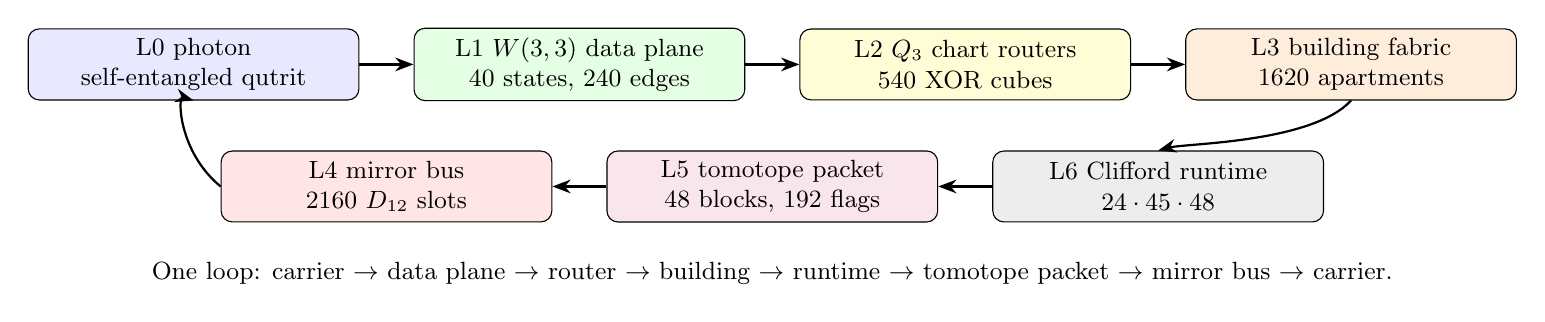
\begin{tikzpicture}[
  every node/.style={font=\small},
  layer/.style={draw,rounded corners,align=center,minimum width=42mm,minimum height=9mm},
  arrow/.style={-{Stealth},thick}
]
  \node[layer,fill=blue!9] (l0) at (0,0) {L0 photon\\ self-entangled qutrit};
  \node[layer,fill=green!10] (l1) at (4.9,0) {L1 $\W$ data plane\\ 40 states, 240 edges};
  \node[layer,fill=yellow!16] (l2) at (9.8,0) {L2 $Q_3$ chart routers\\ 540 XOR cubes};
  \node[layer,fill=orange!14] (l3) at (14.7,0) {L3 building fabric\\ 1620 apartments};
  \node[layer,fill=red!10] (l4) at (2.45,-1.55) {L4 mirror bus\\ 2160 $D_{12}$ slots};
  \node[layer,fill=purple!10] (l5) at (7.35,-1.55) {L5 tomotope packet\\ 48 blocks, 192 flags};
  \node[layer,fill=gray!14] (l6) at (12.25,-1.55) {L6 Clifford runtime\\ $24\cdot45\cdot48$};
  \draw[arrow] (l0) -- (l1);
  \draw[arrow] (l1) -- (l2);
  \draw[arrow] (l2) -- (l3);
  \draw[arrow] (l3.south) .. controls (14.2,-1.0) and (12.6,-1.0) .. (l6.north);
  \draw[arrow] (l6) -- (l5);
  \draw[arrow] (l5) -- (l4);
  \draw[arrow] (l4.west) .. controls (-0.2,-1.1) and (-0.2,-0.4) .. (l0.south);
  \node[align=center,font=\small] at (7.35,-2.65)
    {One loop: carrier $\rightarrow$ data plane $\rightarrow$ router $\rightarrow$ building
    $\rightarrow$ runtime $\rightarrow$ tomotope packet $\rightarrow$ mirror bus $\rightarrow$ carrier.};
\end{tikzpicture}}
\caption{The photonic holonet as an engineering stack.  The same photon
is data, instruction, and packet; the same finite geometry supplies the
network, middleware, and runtime.}
\end{figure}

%======================================================================
\section{The substrate}
\label{sec:substrate}

\begin{definition}[$\W$]
Let $V=\GF3^4$ with the alternating form
$\langle u,v\rangle = u_1v_3-u_3v_1+u_2v_4-u_4v_2$.  The points of
$\W$ are the $40$ projective points of $V$; the lines are the $40$
totally isotropic projective lines.  Each point lies on $4$ lines and
each line carries $4$ points; collinearity defines the strongly regular
graph $\mathrm{SRG}(40,12,2,4)$.
\end{definition}

Three related symmetry groups occur, and their roles are different:
\[
\underbrace{\Sp(4,3)}_{2\cdot\PSp(4,3)\text{, Clifford double cover}},
\qquad
\underbrace{\PSp(4,3)}_{25920\text{, faithful projective action}},
\qquad
\underbrace{W(E_6)\cong\PSp(4,3){:}2}_{51840\text{, outer Weyl extension}}.
\]
The first and third groups both have order $51840$ but are not the
same extension: the center of $\Sp(4,3)$ acts trivially on projective
points and lines, while the outer involution in $W(E_6)$ acts
nontrivially.  The projective group acts with permutation rank $3$.
The ATLAS index-$40$ subgroups are the two building parabolics
$3^{1+2}{:}2A_4$ and $3^3{:}S_4$ \cite{atlasu42}.  The substrate
primitives are
\[
q=3,\quad \lambda=2,\quad \mu=4,\quad k=12,\quad f=24,\quad g=15,\quad
\Phi_6=7,\quad \Phi_4=10,\quad \Phi_3=13,
\]
and every numerical claim in this paper reduces to arithmetic in these.

\paragraph{Formal grounding (the master formalism).}
In the master manuscript \cite{w33paper} the whole structure is forced
by one Diophantine seed: the \emph{master equation} $q! = 2q$ has the
unique positive-integer solution $q=3$, and the SRG quadratic
$x^2 - q!\,x + 2^q = (x-2)(x-4)$ then delivers $\lambda=2$, $\mu=4$ and
the full parameter closure ($k=2^q+q+1$, $v=40$, multiplicities $f=24$,
$g=15$, cyclotomic ladder $\Phi_3=13$, $\Phi_6=7$, $\Phi_{12}=q^4-q^2+1=73$,
$\Theta=q^2+1=10$).  Two of those closure constants reappear in this
paper as \emph{spectral field discriminants}: the chart-web's irrational
eigenvalue pairs $1\pm\sqrt{10}$ and $(-1\pm\sqrt{73})/2$
(\S\ref{sec:network}) live precisely in $\mathbb{Q}(\sqrt{\Theta})$ and
$\mathbb{Q}(\sqrt{\Phi_{12}})$ --- the machine's transport spectrum
speaks the same cyclotomic dialect as the physics tier ladder.

\subsection{The two carriers and the operator--operand duality}
\label{sec:duality}

\begin{theorem}[Two realizations, one geometry]
\label{thm:duality}
\textup{(i)} The $40$ Witting rays in $\mathbb{C}^4$ (the photon's
path$\,\otimes\,$polarization space) have orthogonality graph
isomorphic to the collinearity graph of $\W$.
\textup{(ii)} The $40$ projective classes of two-qutrit Pauli
displacements $D(v)=X^{a}Z^{b}\!\otimes\!X^{c}Z^{d}$ on $\mathbb{C}^9$
(the photon's past$\,\otimes\,$future time-bin space) have commutation
graph equal to the same $\W$, via
$D(u)D(v)=\omega^{\langle u,v\rangle}D(v)D(u)$.
\emph{Witnesses: \path{bt817_self_entangled_photon_atlas.py},
\path{bt821_operator_operand_duality.py}.}
\end{theorem}

Thus a point of the substrate is simultaneously a pure state the photon
can occupy and a unitary the photon can enact; a line is simultaneously
a measurement context (orthonormal tetrad) and a stabilizer group
(maximal commuting Pauli set with its $9$-state joint eigenbasis).  The
$360 = 40\times 9 = f\cdot g$ two-qutrit stabilizer states are the
joint eigenbases of the forty lines.

\subsection{The five vacua and the Schl\"afli geography}

Every maximal subgroup class of $\PSp(4,3)$ decomposes the substrate
in its own canonical way; the maximal indices are the classical
inventory of the $27$ lines on a cubic surface.

\begin{center}\small
\begin{tabular}{llllll}
\toprule
index & subgroup & points & lines & vacuum & cubic surface\\
\midrule
27 & $2^4{:}A_5$ & $[40]$ & $[40]$ & homogeneous (icosahedral) & 27 lines\\
36 & $S_6$ & $[40]$ & $[10,30]$ & spread fibration & 36 double-sixes\\
40 & parabolic & $[1,12,27]$ & $[4,36]$ & holonet point vacuum & trihedra I\\
40 & parabolic & $[4,36]$ & $[1,12,27]$ & dual line vacuum & trihedra II\\
45 & $(2T{\times}2T){:}2$ & $[8,32]$ & $[16,24]$ & binary polar & 45 tritangents\\
\bottomrule
\end{tabular}
\end{center}

The physical decomposition $40=1+12+27$ (self + gauge shell + matter
shell) is the \emph{choice of the point-parabolic vacuum} among five
inequivalent readings; the icosahedral vacuum sees a featureless
substrate.  The platonic ladder threads the table: the binary
tetrahedral group $2T$ (the $24$-cell) lives in every polar-pair
stabilizer, the real octahedral group $O_h$ ($=S_4\times\mathbb Z_2$,
order $48$) is the chart symmetry of \S\ref{sec:network}, and the
binary icosahedral group $2I=\mathrm{SL}(2,5)$ (the $600$-cell) is the
core of every spread stabilizer, with point orbits $[20,20]$ and line
orbits $[10,30]$ echoing the Boerdijk--Coxeter decomposition
$600=20\times 30$.
\emph{Witnesses: \texttt{bt808--bt813}.}

\subsection{The parabolic router: address and route are dual}
\label{sec:parabolic-router}

The two index-$40$ parabolics are not duplicate descriptions of one
local neighborhood.  They execute different halves of a packet
protocol.  This becomes visible only after the compass census: there
are two $216$-element classes of icosahedral $A_5$ cores, and exactly
$1296=216\cdot6$ cross-class pairs meet in $D_{10}$.

\begin{theorem}[Bell--compass parabolic router]
\label{thm:parabolic-router}
Fix an isotropic Bell line.  Its projective Siegel parabolic
$3^3{:}S_4$ has four orbits on the $1296$ incident compass pairs:
\[
162_L+162_R+324+648.
\]
They are distinguished objectwise by the Bell line lying in the
pentad core's $5_L$, $5_R$, $10$, or $20$ line orbit.  The normalized
orbit sizes satisfy the Kraft equality
\[
2^{-3}+2^{-3}+2^{-2}+2^{-1}=1,
\]
so they admit the complete prefix decoder
\[
110\mapsto\text{left cache},\quad
111\mapsto\text{right cache},\quad
10\mapsto\text{schedule},\quad
0\mapsto\text{dark mirror}.
\]
The outer Weyl involution fuses exactly the two $162$ cache orbits,
leaving $324_{\rm cache}+324_{\rm schedule}+648_{\rm mirror}$.
By contrast, the dual point parabolic has two regular projective
orbits of size $648$; the outer extension preserves rather than fuses
these address sheets.
\emph{Witness: \path{bt859_bell_compass_parabolic_router.py}.}
\end{theorem}

The equality case of Kraft--McMillan means the routing words fill a
binary decision tree with no unused branch \cite{mcmillan}.  Here the
code lengths were not optimized from assumed traffic probabilities:
they were read from exact group orbits.  A packet first asks whether
its Bell line is in the dark mirror half; if not, whether it is in the
common schedule quarter; only the remaining cache quarter needs the
third, chiral bit.  The decoder is self-delimiting and constant-depth,
with expected word length
\[
\frac12(1)+\frac14(2)+2\cdot\frac18(3)=\frac74
\]
under the invariant uniform measure on the $1296$ compass pairs.

\begin{center}\small
\begin{tabular}{rlll}
\toprule
orbit & Bell-line position & prefix & engineering action\\
\midrule
$648$ & dark $20$-orbit & $0$ & enter mirror bus\\
$324$ & common schedule $10$-orbit & $10$ & timetable-local route\\
$162$ & absolute pentad $5_L$ & $110$ & left cache\\
$162$ & absolute pentad $5_R$ & $111$ & right cache\\
\bottomrule
\end{tabular}
\end{center}

\begin{figure}[ht]\centering
\resizebox{0.96\textwidth}{!}{%
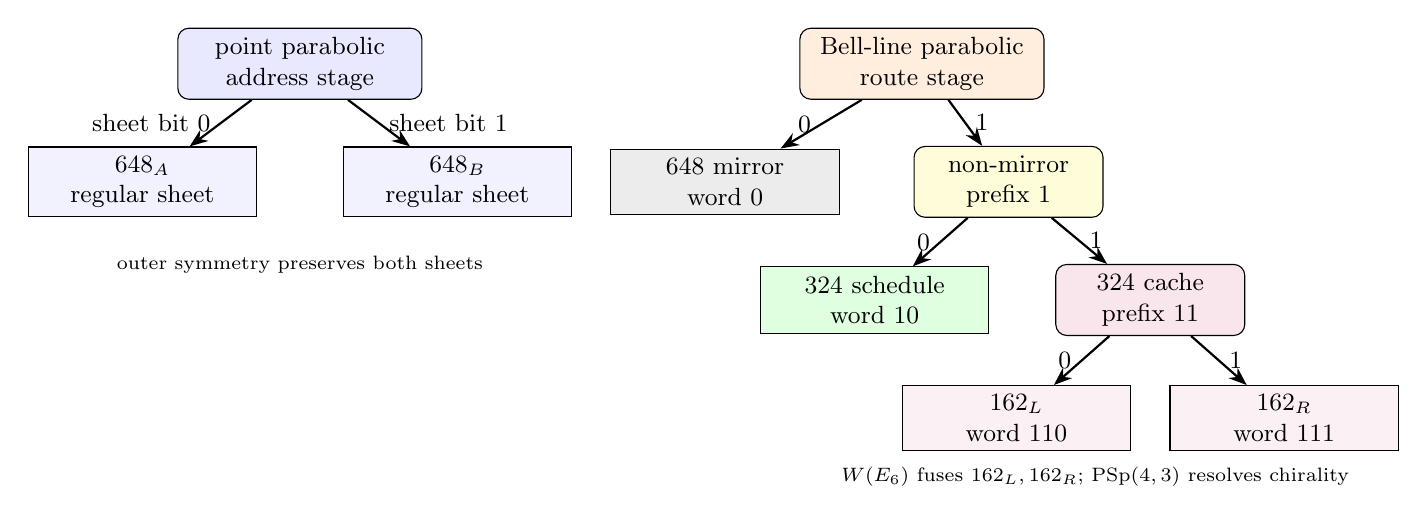
\begin{tikzpicture}[
  every node/.style={font=\small,align=center},
  box/.style={draw,rounded corners,minimum width=31mm,minimum height=9mm},
  leaf/.style={draw,minimum width=29mm,minimum height=8mm},
  arr/.style={-{Stealth},thick}
]
  \node[box,fill=blue!9] (point) at (-0.5,2.0)
    {point parabolic\\address stage};
  \node[leaf,fill=blue!5] (pa) at (-2.5,0.5) {$648_A$\\regular sheet};
  \node[leaf,fill=blue!5] (pb) at (1.5,0.5) {$648_B$\\regular sheet};
  \draw[arr] (point) -- node[left] {sheet bit $0$} (pa);
  \draw[arr] (point) -- node[right] {sheet bit $1$} (pb);
  \node[font=\scriptsize] at (-0.5,-0.55)
    {outer symmetry preserves both sheets};

  \node[box,fill=orange!13] (line) at (7.4,2.0)
    {Bell-line parabolic\\route stage};
  \node[leaf,fill=gray!15] (mirror) at (4.9,0.5) {$648$ mirror\\word $0$};
  \node[box,fill=yellow!15,minimum width=24mm] (rest) at (8.5,0.5)
    {non-mirror\\prefix $1$};
  \node[leaf,fill=green!12] (sched) at (6.8,-1.0) {$324$ schedule\\word $10$};
  \node[box,fill=purple!10,minimum width=24mm] (cache) at (10.3,-1.0)
    {$324$ cache\\prefix $11$};
  \node[leaf,fill=purple!6] (left) at (8.6,-2.5) {$162_L$\\word $110$};
  \node[leaf,fill=purple!6] (right) at (12.0,-2.5) {$162_R$\\word $111$};
  \draw[arr] (line) -- node[left] {$0$} (mirror);
  \draw[arr] (line) -- node[right] {$1$} (rest);
  \draw[arr] (rest) -- node[left] {$0$} (sched);
  \draw[arr] (rest) -- node[right] {$1$} (cache);
  \draw[arr] (cache) -- node[left] {$0$} (left);
  \draw[arr] (cache) -- node[right] {$1$} (right);
  \node[font=\scriptsize] at (9.6,-3.25)
    {$W(E_6)$ fuses $162_L,162_R$; $\PSp(4,3)$ resolves chirality};
\end{tikzpicture}}
\caption{The two $C_2$ parabolics implement a dual protocol.  Point
localization selects one of two address torsors; Bell-line localization
decodes a complete variable-length route word.}
\label{fig:parabolic-router}
\end{figure}

This theorem also closes an honesty boundary.  The Bell stabilizer and
the compass incidence set both have cardinality $1296$, but they are
not a regular $G$-set identification.  Projectively, the Bell
stabilizer has order $648$ and the orbit stabilizers are $1,2,4$.
The useful result is stronger than the count: a hierarchical decoder
and a persistent address bit are forced by the two parabolic actions.

\subsection{The incidence transceiver and the route-dark lattice}
\label{sec:incidence-transceiver-route-dark}

Pass~173 turns the address/route distinction into an exact signal law.
For the line--point incidence matrix $N$, the centered operator
\[
 T=N-\frac1{10}J
\]
has rank $24$ and satisfies
\[
 TA_P=A_LT,
 \qquad T^{\mathsf T}T=6E_{24}^{P},
 \qquad TT^{\mathsf T}=6E_{24}^{L}.
\]
Thus $T/\sqrt6$ is a lossless transceiver on the shared gauge sector,
while the unmatched address and route dark sectors remain type-protected.
Every one of the $480$ local-axis selector vectors produces a
$40$-channel analyzer word with histogram
$\{-3^1,-1^9,0^{20},1^9,3^1\}$ and exact decoder
$x=N^{\mathsf T}(Nx)/6$.

The two dark lattices are not interchangeable.  The address lattice
$\ker_{\mathbb Z}N$ has minimum shell $90$ at norm $8$ and binary code
$[40,15,8]$; the route-dark lattice $\ker_{\mathbb Z}N^{\mathsf T}$ has
minimum shell $432$ at norm $10$ and code $[40,15,10]$.  Its $216$
projective supports are exactly the pentad cores already used by the
router: each is $K_{5,5}$ minus a perfect matching, and the deleted
matchings double-cover the $540$ skew-line chart atlas.  The signed shell
splits into the two chiral $216$-orbits.  Hence the old compass carrier is
not merely count-compatible with the route layer; it is its complete
minimum-energy integral dark shell.

The two $25$-dimensional context duals are locally indistinguishable at
their first two nonzero shells: both have $A_4=40$ and $A_6=240$.  They
first separate at the third shell,
\[
 A_8^{\rm address}=5085,
 \qquad A_8^{\rm route}=3645.
\]
Moreover only the address code is self-orthogonal; the route code has
binary Gram rank $6$.  Thus the Pass-164 $O^+(10,2)$ quotient is
address-chiral and cannot be silently reused as a route codec.

This also corrects the architecture vocabulary.  At odd $q=3$,
$W(3,3)$ and its dual $Q(4,3)$ have equal $40+40$ counts and cospectral
concurrence graphs, but are not incidence-self-dual.  The lossless
identification exists only on the shared $24$-sector.  The statement is
an algebraic analyzer-ROM/control-codec theorem until a specified optical
amplitude implementation of $T$ is supplied.  (Witness:
\path{analysis/w33_pass173_incidence_transceiver_route_dark_lattice.py}.)

Pass~174 supplies the missing protected subcodec.  Although the full
route code $R=[40,15,10]$ is not self-orthogonal, its route-code hull is
\[
 H=R\cap R^\perp=[40,9,16],
 \qquad
 W_H=1+135z^{16}+240z^{20}+135z^{24}+z^{40}.
\]
The all-ones word is a fixed radical and
$H/\langle\mathbf1\rangle$ is a plus-type $8$-space with the exact
$1+135+120$ native group orbits.  Its $255$ nonzero words reconstruct
the symplectic graph $\SRG(255,126,61,63)$ and its two quadratic
subconstituents $\SRG(135,70,37,35)$ and
$\SRG(120,63,30,36)$.  So one route codec now supplies the complete
finite stack
\[
 432\text{ signed pentads}\to216\text{ cores}\to[40,9,16]
 \to255=135+120.
\]

The order-eight control rail is also less obstructed than the previous
cohomology wording claimed.  On both address and route discriminants,
$[\tau(h)-h]=0$ while
$[\tau(h)-5h]=[4h]\ne0$.  Thus a $q(h)=11/8$ fixed order-eight rail
exists; the nonzero class forbids only a pure scalar-$5$ normal form.
This is a finite control-label theorem, not yet a fabricated phase rail.
(Witness: \path{analysis/w33_pass174_dual_discriminant_fixed_rail.py}.)

Pass~176 removes the remaining abstract quotient choice.  If
$C=\ker_{\mathbb F_2}N$ and $R=\ker_{\mathbb F_2}N^{\mathsf T}$, the
unique nonzero fixed isotropic class $f\in C^\perp/C$ is sent by incidence
to the all-ones route word, and
\[
 f^\perp/\langle f\rangle
 \xrightarrow{\;N\;}
 (R\cap R^\perp)/\langle\mathbf1\rangle
\]
is an exact native-$\PSp(4,3)$ quadratic isometry.  All $512$ quadratic
identities and $8192$ generator/object commuting squares are checked.
The $240$ weight-six address words become the two explicit sheets over
the $120$ anisotropic route states and map bijectively to the $240$
weight-$20$ hull words.  This is an executable codec map; it still does
not specify an optical transfer matrix, loss budget, or detector model.

Pass~177 then locates the first address/route classification depth in the
\emph{dual} context lattices.  Both begin
\[
 1+720q^2+15360q^3,
\]
where the $720$ is coordinate doubles plus sign-lifts of lines on the
address side and point stars on the route side.  They first split at
\[
 q^4:\qquad 1350960-982320=368640.
\]
Thus firmware may share the first two dual-shell tables, but must retain
the type bit before admitting weight-eight sectors.  Separately, the
sentinel/context theta regression has an exact normalization because
$A^\vee=\tfrac12B$ and $\operatorname{covol}(A)=2^{25}$; finite shell sums
are regression checks only.  Finally,
$\ker_{\mathbb Z}N^{\mathsf T}$ is the point-trade lattice of the
nonisomorphic dual $Q(4,3)$, whose span size is $2$ versus $4$ for
$W(3,3)$.  A route generator with $q=11/8$ exists, but $3/8$ occurs on
the other fixed-generator orbit, so no invariant $11/8$ hardware phase
is inferred.  (Witnesses:
\path{analysis/w33_pass176_incidence_fixed_line_e8_bridge.py},
\path{analysis/w33_pass177_address_route_dual_theta_split.py}, and
\path{analysis/w33_pass179_poisson_modular_pair.py}.)

Passes~188--192 refine the local controller geometry.  The $432$ route
minima contain $36$ exact double-six crowns: each is
$K_{6,6}$ minus a matching, assembled from one $K_6$ in each of the two
chiral shell orbits, with faithful $S_6$ component symmetry.  The naive
homogeneous-product scheduler is ruled out:
\[
 (120\ \text{axes})\times(36\ \text{double-sixes})
 =3240+720+360=120(27+6+3).
\]
Thus a packet carrying an axis/double-six pair needs a three-valued
relation-type tag; the $4320$ pairs are not one native group orbit.  The
positive replacement is local: an axis stabilizer of order $216$ acts on
its distinguished three double-sixes through full $S_3$ with kernel $36$,
giving a genuine $S_3/C_2$ completion fibre.

Restoring signs gives an even sharper codec.  The three positive octads
of each signed second-shell trade contain a unique two-point edge of its
matched four-point line; the three negative octads contain the
complementary edge.  Hence
\[
 240\ \text{signed trades}\longleftrightarrow40\ \text{lines}\times6\
 \text{edge addresses},
\]
with sign reversal implemented by edge complement.  The line stabilizer
satisfies $1\to C_3^3\to H_{\rm line}\to S_4\to1$: its six signed states
carry the tetrahedral-edge $S_4$ action, while complement-pairing gives
the unframed $S_3/C_2$ axis action.  Firmware must therefore not identify
the six edge states with a regular $S_3$ clock merely because both sets
have size six.  (Witnesses:
\path{analysis/w33_pass188_icosahedron_test.py},
\path{analysis/w33_pass191_supercycle_pullback.py}, and
\path{analysis/w33_pass192_signed_trade_edge_s4.py}.)

Passes~209--212 close the global controller carrier without undoing that
local warning.  A route-shell double-six $D$ now determines its timetable
intrinsically:
\[
 \Sigma(D)=\{\ell:\ v_\ell=0\ \hbox{for every signed minimum }v\in D\}.
\]
The ten lines in $\Sigma(D)$ are pairwise skew and cover all $40$ points;
the $36$ double-sixes recover all $36$ spreads, equivariantly and
bijectively.  On the crossing-pair six-set of $D$, its ten silent lines are
the ten unordered $3+3$ bisections, by a unique $S_6$-equivariant atlas.
The associated doily is the derived duad--syntheme geometry on that six-set,
not a literal incidence subgeometry on the twelve crown vertices.

This bridge gives the controller an exact two-stratum ABI.  For a silent
spread incidence $(\Sigma,\ell)$, the common stabilizer has order $72$ and
shape $(S_3\times S_3){:}C_2$; its line-clock image is $C_2$ with kernel
$S_3\times S_3$.  For an active pair $\ell\notin\Sigma$, the stabilizer is
$S_4$, faithful on the four points of $\ell$, and its line-clock quotient is
$S_4/V_4\cong S_3$.  Thus the silent and active rows require an explicit
stratum bit: they are two equivariant clock modes, not one direct-product
clock.

Most importantly, the previously numerical $4320$-carrier coincidence is
now a canonical $\PSp(4,3)$-equivariant bijection.  Let
\[
 X=\{(\Sigma,L,p):L\notin\Sigma,\ p\in L\},\qquad
 |X|=1080\cdot4=4320.
\]
For $(\Sigma,L,p)$, let $M$ be the unique line of $\Sigma$ through $p$ and
let $N$ be the unique line meeting $M$, disjoint from $L$, whose four
$\Sigma$-owner lines equal those of $L$.  Then
\[
 (\Sigma,L,p)\longmapsto(L,M,N)
\]
is the required bijection to ordered nonlocal two-paths; the inverse chooses
the unique such $\Sigma$ and returns $p=L\cap M$.  The path has three
quadrangle completions, canonically indexed by the other three points of
$L$, so the complete incidence surface is
\[
 1080\cdot4\cdot3=12960.
\]
In the full $\mathrm{PGSp}(4,3)$ supercycle the path stabilizer is the split
group $S_3\times C_2$ of order $12$: $S_3$ permutes the three completions,
its central kernel has order two, and fixing one completion leaves $V_4$.
That $V_4$ is an exact four-element branch carrier, but it is \emph{not} a
regular four-probe address on the completion line: the four points have
orbits $1+1+2$.  Firmware must supply any semantic probe-role labelling
separately rather than infer it from group order.  (GAP witnesses:
\path{analysis/w33_pass209_silent_spread_two_clock.g},
\path{analysis/w33_pass210_s6_route_atlas.g},
\path{analysis/w33_pass211_pgsp_controller_clifford.g}, and
\path{analysis/w33_pass212_4320_carrier_equivariant_bijection.g}.)

Passes~214--218 now separate the remaining controller sheets before any
optical interpretation.  The four points of the \emph{source} line do carry
a regular $V_4$ action: after choosing the source point, the identity fixes
that port and the three nonidentity double transpositions address the other
ports through their intrinsic pair-partition labels.  This is the exact
four-way switching algebra that the completion line lacked, but the residual
$S_3$ still permutes the three nonidentity labels.  A photonic controller
must calibrate semantic port names; geometry supplies the torsor, not the
laboratory naming convention.

The same carrier sheet selects the local-axis endpoint formed by the external
line and its unique spread owner through the source point.  GAP verifies the
uniform tower
\[
 4320\xrightarrow{18:1}240\xrightarrow{2:1}120,
\]
where endpoint complement is a fixed-point-free $C_2$ deck operation central
in the extended order-$103680$ action.  Via Pass~123's chosen chamber gauge it
can be represented by an $E_8$ root sign; it is not a measured optical phase.
Moreover the transitive W33-code action and the standard
$E_6\times A_2<E_8$ branching action are nonconjugate and have different
root-orbit fingerprints, so choosing rational $E_8$ coordinates remains a
chamber calibration rather than a symmetry-forced device frame.

Incidence duality also changes the schedule type.  $W(3,3)$ has $36$ spreads
and no ovoids, while $Q(4,3)$ has no spreads and $36$ ovoids; the duality-odd
checksum is therefore
$\Delta_{SO}=\#\mathrm{spreads}-\#\mathrm{ovoids}=\pm36$, not an Euler
characteristic.  The surviving $Q$ carrier
is the ovoid tower $4320=36\cdot15\cdot2\cdot4$ with stabilizers
$S_6>C_2\times S_4>S_4>S_3$.  It is the incidence-dual typing of the same
controller, not a second independent optical channel, and its central mate
swap is not an absolute handedness observable.

The construction is also special to field order three.  At the tested odd
anchors the regular-spread owner router covers the path carrier with degree
$(q-1)/2$:
$1,2,3$ at $q=3,5,7$, so only $q=3$ is lookup-free and bijective.  The module
backend changes at the same anchors: the $q=5$ binary $24$ is the
$\mathbb F_2$ restriction of an $\mathbb F_4$ Weil $12$, while the $q=7$
$48$ is the split dual pair $24\oplus24^*$.  These are representation and
control-plane constraints, not claims of fabricated modes or measured
coherence.  (GAP witnesses:
\path{analysis/w33_pass214_source_line_v4_torsor.g},
\path{analysis/w33_pass215_carrier_double_six_signed_e8.g},
\path{analysis/w33_pass216_q43_dual_ovoid_carrier.g},
\path{analysis/w33_pass217_w3q_owner_spread_uniqueness.g}, and
\path{analysis/w33_pass218_weil_shadow_split.g}.)

%======================================================================
\section{The carrier: how to self-entangle a photon}
\label{sec:carrier}

Entanglement is a relation between tensor factors; nothing requires
the factors to be distinct particles.  Self-entanglement is
entanglement between one photon's own registers.

\subsection{Stage A: spatial (one element)}
A diagonal photon meets a polarizing beam splitter:
$\tfrac1{\sqrt2}(\ket{H}+\ket{V})\ \mapsto\
\tfrac1{\sqrt2}(\ket{H,a}+\ket{V,b})$.
Path and polarization are now maximally entangled \emph{within} the
photon; this two-qubit $\mathbb{C}^4$ is the Witting carrier of
Theorem~\ref{thm:duality}(i).

\subsection{Stage B: temporal (two Clifford gates)}
A tritter (symmetric $3$-port coupler) \emph{is} the qutrit Fourier
gate $F_3$; a three-bin delay ladder ($0,\tau,2\tau$) defines past and
future registers; one electro-optic modulator applies
$\mathrm{CX}_{p\to f}$ conditioned on bin index.  The temporal Bell
qutrit
\[
\ket{\Omega}\;=\;\mathrm{CX}_{p\to f}\,(F_3\otimes I)\ket{0}_p\ket{0}_f
\;=\;\frac1{\sqrt3}\sum_{j=0}^{2}\ket{j}_p\ket{j}_f
\]
is verified exactly; the photon is entangled with its own future.
Inserting any $U$ in the future arm, the recombination visibility is
the \emph{trace--Choi witness}
\[
V(U)\;=\;\frac{|\mathrm{Tr}\,U|}{3},\qquad
V(F_3)=\tfrac13,\quad V(X)=V(Z)=0,
\]
so the photon implements the Choi--Jamio{\l}kowski isomorphism on
itself: it measures channels against its own past.
\emph{Witness: \path{bt820_self_entanglement_protocol.py}.}

\begin{figure}[ht]\centering
\resizebox{\textwidth}{!}{%
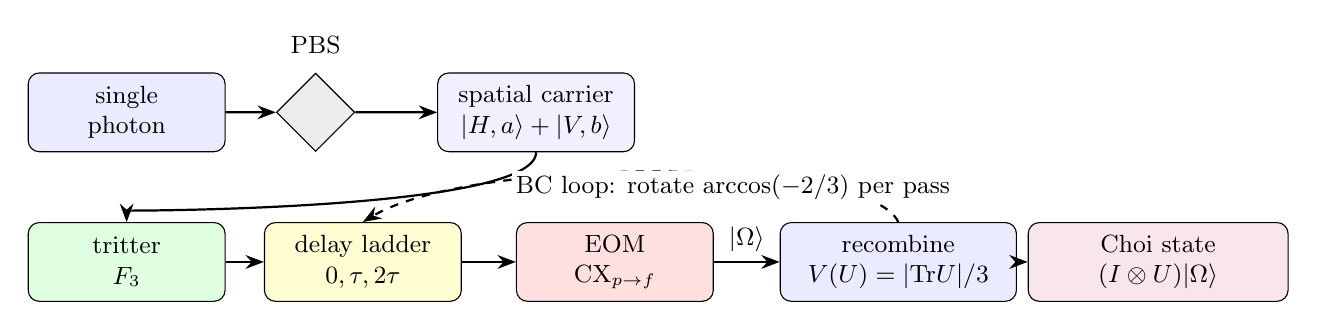
\begin{tikzpicture}[
  every node/.style={font=\small},
  block/.style={draw,rounded corners,align=center,minimum width=25mm,minimum height=10mm},
  optic/.style={draw,align=center,fill=gray!15,minimum width=16mm,minimum height=10mm},
  arrow/.style={-{Stealth},thick}
]
  \node[block,fill=blue!8] (src) at (0,0) {single\\photon};
  \node[draw,fill=gray!15,minimum width=7mm,minimum height=7mm,
        rotate=45,inner sep=0pt] (pbs) at (2.4,0) {};
  \node[font=\small] at (2.4,0.85) {PBS};
  \node[block,fill=blue!6] (spatial) at (5.2,0)
    {spatial carrier\\ $\ket{H,a}+\ket{V,b}$};
  \node[block,fill=green!12] (tri) at (0,-1.9) {tritter\\ $F_3$};
  \node[block,fill=yellow!18] (delay) at (3.0,-1.9) {delay ladder\\ $0,\tau,2\tau$};
  \node[block,fill=red!12] (eom) at (6.2,-1.9) {EOM\\ $\mathrm{CX}_{p\to f}$};
  \node[block,fill=blue!8,minimum width=30mm] (out) at (9.8,-1.9)
    {recombine\\ $V(U)=|\mathrm{Tr}U|/3$};
  \node[block,fill=purple!10,minimum width=33mm] (choi) at (13.1,-1.9)
    {Choi state\\ $(I\otimes U)\ket{\Omega}$};
  \draw[arrow] (src) -- (pbs);
  \draw[arrow] (pbs) -- (spatial);
  \draw[arrow] (spatial.south) .. controls (5.2,-1.25) and (0,-1.25) .. (tri.north);
  \draw[arrow] (tri) -- (delay);
  \draw[arrow] (delay) -- (eom);
  \draw[arrow] (eom) -- (out) node[midway,above]{$\ket{\Omega}$};
  \draw[arrow] (out) -- (choi);
  \draw[-{Stealth},dashed,thick] (out.north) .. controls (9.4,-0.55) and (4.4,-0.55) ..
    (delay.north);
  \node[fill=white,inner sep=1.5pt,font=\small] at (7.7,-0.95)
    {BC loop: rotate $\arccos(-2/3)$ per pass};
\end{tikzpicture}}
\caption{Preparation schematic.  One photon, four registers.  The PBS
entangles path with polarization (Stage A); the tritter--delay--EOM
chain prepares the temporal Bell qutrit $\ket{\Omega}$ (Stage B); the
dashed loop is the irrational Boerdijk--Coxeter drive of
\S\ref{sec:time}.}
\end{figure}

%======================================================================
\section{The network: atlas, building, and routing}
\label{sec:network}

\begin{theorem}[The hypercube atlas]
$\W$ contains exactly $540$ skew line pairs.  For each pair the
non-collinearity graph on its $8$ points is the cube graph $Q_3$, with
full symmetry group $O_h$ of order $48$ (these are the only
order-$48$ stabilizers; the binary $2O$ does not occur).  Each chart
admits an exact $\GF2^3$ Gray-code addressing in which chart edges are
unit XOR moves and the antipode of a vertex is its unique collinear
partner.  Every $\W$ nonedge is a chart edge in exactly $12=k$ charts;
every edge is an antipode pair in exactly $9=q^2$.
\emph{Witnesses: \texttt{bt773}, \texttt{bt777}, \texttt{bt778}.}
\end{theorem}

\subsection{Hypercube networking, not hypercube decoration}

The cube is not only a picture for one chart.  It is the local
interconnect primitive.  A chart gives eight simultaneously valid
addresses
\[
000,\ 001,\ 010,\ 011,\ 100,\ 101,\ 110,\ 111\in\GF2^3,
\]
and the elementary network instruction is the dimension-order
hypercube hop
\[
a\longmapsto a\oplus e_i,\qquad i\in\{1,2,3\}.
\]
This is the standard e-cube rule of hypercube networks: compare source
and target, flip one differing coordinate at a time, and finish in at
most three local hops \cite{saadschultz}.  In the holonet that same XOR flip is also a
register operation, because the chart address is a finite
``which-register'' word on the photon's self-entangled carrier.  The
local routing primitive is therefore simultaneously
\[
\hbox{bit flip}\quad=\quad\hbox{qutrit-frame update}\quad=\quad
\hbox{optical path choice}.
\]

A packet in the photonic holonet is not merely a payload.  The natural
packet header is
\[
\mathcal{P}=(\hbox{payload},\ \hbox{Pauli frame},\ \hbox{chart word},
\ \hbox{apartment hop},\ \hbox{mirror slot},\ \hbox{clock phase}).
\]
The payload is the quantum state or teleported gate; the Pauli frame is
the two-trit feedforward record; the chart word is the $\GF2^3$ route
inside the current cube; the apartment hop selects the next chart; the
mirror slot chooses the $D_{12}$ transport bus of
\S\ref{sec:middleware}; and the clock phase is the cyclic $C_{12}$
interrupt that keeps the selector coherent.  This is why the same
object can be called a computer architecture and a network
architecture.  A node never sends data to a processor: the act of
transport is the processor's gate action.

\begin{theorem}[The fabric is the building]
The chart-adjacency web ($540$ nodes, two charts adjacent when one's
axis is a disjoint transversal pair of the other) is $6$-regular with
exactly $1620$ edges, and these edges are in canonical bijection with
the $1620$ apartments of the Tits building of $\Sp(4,\GF3)$.  The web
has diameter $5$; its adjacency module contains the Steinberg
representation twice and presses against the Ramanujan bound only on a
$15$-dimensional sentinel eigenspace.
\emph{Witnesses: \texttt{bt777}, \texttt{bt779}, \texttt{bt744}.}
\end{theorem}

\begin{figure}[ht]\centering
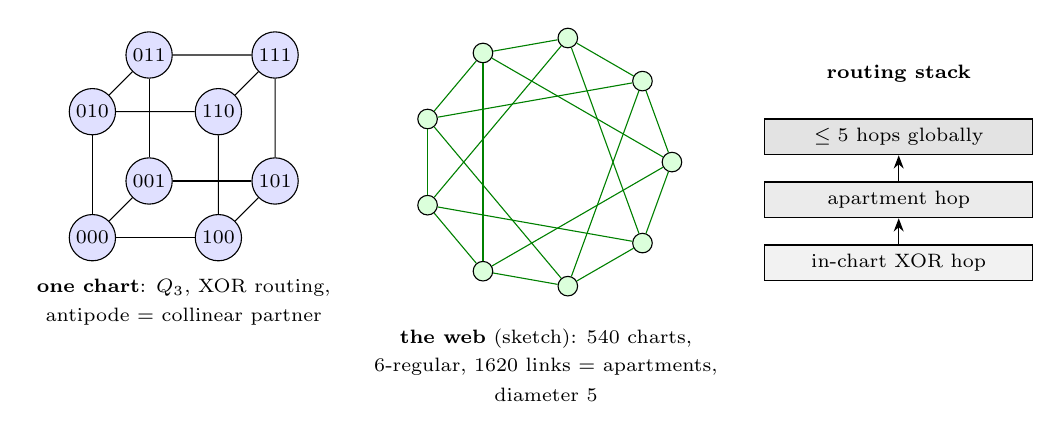
\begin{tikzpicture}[scale=0.8, every node/.style={font=\scriptsize}]
  % one chart cube
  \foreach \x/\y/\n/\l in {0/0/000/000, 2/0/100/100, 0/2/010/010,
    2/2/110/110, 0.9/0.9/001/001, 2.9/0.9/101/101, 0.9/2.9/011/011,
    2.9/2.9/111/111}{
    \node[circle,draw,fill=blue!12,inner sep=1.5pt] (\n) at (\x,\y) {\l};}
  \foreach \a/\b in {000/100,000/010,000/001,100/110,100/101,010/110,
    010/011,001/101,001/011,110/111,101/111,011/111}{
    \draw (\a) -- (\b);}
  \node at (1.45,-0.8) {\textbf{one chart}: $Q_3$, XOR routing,};
  \node at (1.45,-1.25) {antipode $=$ collinear partner};
  % web
  \begin{scope}[xshift=7.2cm,yshift=1.2cm]
    \foreach \i in {0,...,8}{
      \node[circle,draw,fill=green!14,inner sep=2.5pt]
        (w\i) at ({360/9*\i}:2.0) {};}
    \foreach \i in {0,...,8}{
      \pgfmathtruncatemacro{\j}{mod(\i+1,9)}
      \pgfmathtruncatemacro{\k}{mod(\i+3,9)}
      \draw[green!50!black] (w\i) -- (w\j);
      \draw[green!50!black] (w\i) -- (w\k);}
    \node at (0,-2.8) {\textbf{the web} (sketch): $540$ charts,};
    \node at (0,-3.25) {$6$-regular, $1620$ links $=$ apartments,};
    \node at (0,-3.7) {diameter $5$};
  \end{scope}
  % layer ladder
  \begin{scope}[xshift=12.8cm,yshift=-0.4cm]
    \node[draw,fill=gray!10,minimum width=34mm] (l1) at (0,0)
      {in-chart XOR hop};
    \node[draw,fill=gray!16,minimum width=34mm] (l2) at (0,1.0)
      {apartment hop};
    \node[draw,fill=gray!22,minimum width=34mm] (l3) at (0,2.0)
      {$\le 5$ hops globally};
    \draw[-{Stealth}] (l1) -- (l2);
    \draw[-{Stealth}] (l2) -- (l3);
    \node at (0,3.0) {\textbf{routing stack}};
  \end{scope}
\end{tikzpicture}
\caption{Network schematics.  Left: a single chart with its
$\GF2^3$ addressing (XOR routing native).  Center: the $540$-chart
web whose links are the apartments of the Tits building (sketched as a
circulant fragment).  Right: the two-level routing stack.}
\end{figure}

Routing a packet means choosing XOR moves inside charts and apartment
hops between them; since chart moves \emph{are} register operations
(\S\ref{sec:software}), routing is computation.  At scale the
recursion is the holonet ladder: $40^n$ cores at level $n$, the same
$\mathrm{SRG}(40,12,2,4)$ at every level, with the level-$0$ chart's
$1+12+27$ degree split realized as self pole, gauge shell, and matter
shell of each node.

\begin{corollary}[Two-plane routing bound]
Inside a chart the worst route length is $3$, the diameter of $Q_3$.
Between charts the worst route length is $5$, the diameter of the
apartment web.  One recursive digit of a holonet address therefore
costs at most
\[
3+5=8
\]
reversible transport moves.  BT827 globalizes this to
$8n=8\log_{40}N$ for $N=40^n$ photonic leaves.
\end{corollary}

%======================================================================
\section{The middleware: tomotope mirrors and the runtime bus}
\label{sec:middleware}

\begin{definition}[Tomotope packet]
In this paper the tomotope is used in the only way the finite
calculation currently justifies: as a local middle-layer incidence
packet.  A tomotope packet has four vertex carriers, twelve local edge
axes, sixteen triangular face labels, and forty-eight edge--face
incidence blocks.  The doubled base/shadow fiber gives $192$ flags.
Thus the tomotope is the durable packet format sitting between the
fast cube router and the global mirror bus; it is not introduced as an
ambient continuous torus, and it is not identified with the rectangle
clock.
\end{definition}

The atlas contains two different $2160$-element boundary worlds.  They
must not be collapsed.  The rectangle side is cyclic: its stabilizer is
$C_{12}$ and it supplies the selector's phase clock.  The
chart-transversal side is dihedral: its stabilizer is $D_{12}$ and it
supplies the mirror transport bus.  Equal cardinality is the red
herring; different stabilizer structure is the theorem.

\begin{theorem}[The $D_{12}$ mirror bus]
The $540$ cube charts carry exactly four common-transversal slots each,
so the global chart-transversal space has $540\cdot4=2160$ slots.  The
map
\[
(\hbox{chart},\hbox{ common transversal line})
\longmapsto
(\hbox{chart},\hbox{ antipode pair cut out by that transversal})
\]
is an equivariant bijection onto the atlas antipode-slot space.  Its
projective stabilizer has order $12$ and GAP identifies it as $D_{12}$,
not $C_{12}$.
\emph{Witness: \path{bt815_global_2160_transversal_gset.py}.}
\end{theorem}

Locally, a skew-line chart has four common isotropic transversals.  Read
those four transversals as the four vertex carriers of the tomotope
middle layer.  Each transversal is a $K_4$, and each $K_4$ has three
opposite-edge axes and four triangular faces.  Thus the chart carries
\[
4 \hbox{ vertices},\qquad 4\cdot3=12 \hbox{ edge labels},\qquad
4\cdot4=16 \hbox{ face labels},
\]
and the middle incidence packet has
\[
4\cdot3\cdot4=48
\]
edge--face blocks, with the doubled base/shadow fiber restoring $192$
flags.  This is the local $\langle r_0,r_3\rangle$ tomotope block layer,
not an analogy to a toroidal polyhedron.
\emph{Witness: \path{bt814_tomotope_middle_layer_from_residual_tetrahedra.py}.}

\begin{theorem}[Photonic mirror middleware]
The full optical Clifford runtime factors as
\[
|\Sp(4,\GF3)| = 51840
              = 24\cdot2160
              = 24\cdot45\cdot48.
\]
Here $24=f$ is the full $\Sp(4,3)$ lift of the projective $D_{12}$
mirror-slot stabilizer, $45$ is the hyperbolic polar-pair/tritangent
geography, and $48$ is the local tomotope edge--face middle layer
(also the order of the chart group $O_h$).  Equivalently, the photon is
clocked by the cyclic selector side and routed by the dihedral mirror
side; the complete Clifford group is the lift of that mirror bus through
the tomotope middle carrier.
\emph{Witness: \path{bt826_photonic_mirror_middleware.py}.}
\end{theorem}

This is the architectural closure missing from a bare universality
claim.  The tritter, phase plate, and controlled delay generate the
whole Clifford group, but the group is \emph{organized} as a middleware
stack: full slot stabilizer, global mirror bus, polar vacuum geography,
and tomotope local block.  In software terms, $C_{12}$ is the clock
interrupt, $D_{12}$ is the mirror router, $48$ is the local packet
format, and $24\cdot45\cdot48$ is the finite runtime.

\begin{figure}[ht]\centering
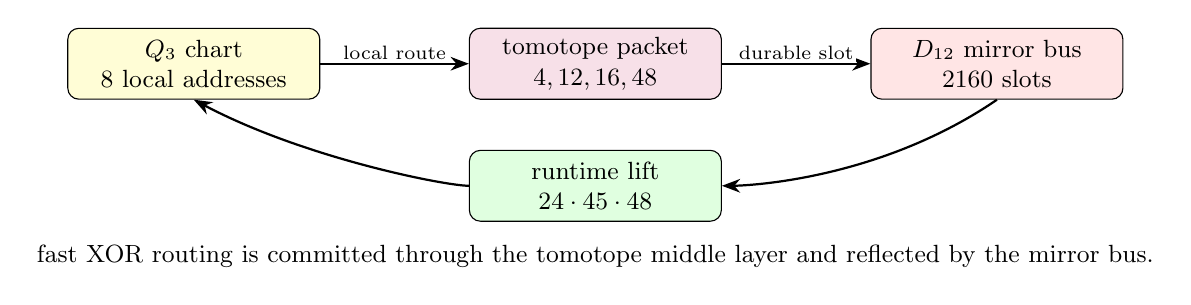
\begin{tikzpicture}[
  every node/.style={font=\small},
  block/.style={draw,rounded corners,align=center,minimum width=32mm,minimum height=9mm},
  arrow/.style={-{Stealth},thick}
]
  \node[block,fill=yellow!16] (cube) at (0,0) {$Q_3$ chart\\ 8 local addresses};
  \node[block,fill=purple!12] (tomo) at (5.1,0) {tomotope packet\\ $4,12,16,48$};
  \node[block,fill=red!10] (mirror) at (10.2,0) {$D_{12}$ mirror bus\\ 2160 slots};
  \node[block,fill=green!12] (runtime) at (5.1,-1.55) {runtime lift\\ $24\cdot45\cdot48$};
  \draw[arrow] (cube) -- node[above,font=\scriptsize,fill=white,inner sep=1pt]{local route} (tomo);
  \draw[arrow] (tomo) -- node[above,font=\scriptsize,fill=white,inner sep=1pt]{durable slot} (mirror);
  \draw[arrow] (mirror.south) .. controls (8.6,-1.55) and (6.8,-1.55) .. (runtime.east);
  \draw[arrow] (runtime.west) .. controls (3.2,-1.55) and (1.4,-1.2) .. (cube.south);
  \node[align=center,font=\small] at (5.1,-2.45)
    {fast XOR routing is committed through the tomotope middle layer and reflected by the mirror bus.};
\end{tikzpicture}
\caption{Middleware schematic.  The cube is the reversible local router;
the tomotope is the edge--face packet format; the $D_{12}$ bus is the
global mirror transport object.}
\end{figure}

% BT1491 exact finite insert stack start
\subsection{Product-grid closure ABI v2}
\label{sec:bt1480-bt1482-product-grid-abi-v2}

The 12 closure strands are modeled as
\[
C_3\times V_4,
\qquad V_4=C_2\times C_2,
\]
rather than as a bare \(C_{12}\).  The \(C_3\) coordinate is the
Szilassi/Fano channel and qutrit phase axis; the \(V_4\) coordinate is the
four-triangle E6 gauge-shell/D4 branch axis.

The E6 firewall square is now upstream in the claim DAG through the exact nodes
\[
36\to72,
\qquad
72+6=78,
\qquad
72+9=81.
\]
This supports the exact finite ABI/CSS branch while leaving blocked formula and
physics claims downstream of the transcription gate.

The closure packet ABI is upgraded to v2.  Each packet carries \(C_3\) channel,
\(V_4\) branch, active/guard outputs, 72-row sector metadata, the nine-mode
firewall gap, and claim-DAG dependencies.

\subsection{ABI v2 consumer, E6 claim table v2, and D4/V4 branch audit}
\label{sec:bt1483-bt1485-abi-v2-d4v4}

The closure ABI v2 is executable.  It regenerates 12 packets, 48 events, and 72
rows while preserving the dual-axis metadata.  The three \(C_3\) channels each
carry 24 rows, and the four \(V_4\) triangles each carry 18 rows.

The E6-merged claim DAG now produces a table with explicit E6 provenance for the
72-sector, the 81 closure, and the \(C_3\times V_4\) grid.  Blocked formula and
physical claims remain downstream.

On branch classes, D4 shear fixes each \(V_4\) triangle, while \(\tau_4\) acts as
an order-two translation preserving the triangle partition as a set.  The two
operations still fail to commute on full branch/phase states, so retwining remains
part of the exact decoder rule.

\subsection{BT1486--BT1488 ABI v2 retwined CSS and splice manifest}
\label{sec:bt1486-bt1488-abi-v2-css-splice}

BT1486 reruns the CSS join from the ABI v2 consumer output.  The result is not
just the old 72-row count: every row satisfies the retwined \(X\)- and
\(Z\)-syndrome checks, while the \(C_3\) channel profile remains
\(P_0=P_1=P_2=24\) rows and the \(V_4\) triangle profile remains
\(T_0=T_1=T_2=T_3=18\) rows.

BT1487 classifies the branch symmetries behind those four triangles.  The full
triangle-partition stabilizer is \(S_4\) of order \(24\), giving the Fano point
reading \(7\cdot24=168\).  The physically used square subgroup is \(D_4\) of
order \(8\), giving the Fano flag reading \(21\cdot8=168\).  Thus the active
detector-bin count is Fano-native, not merely an optical count.

BT1488 updates the splice cascade: the E6 claim table v2 from BT1484 supersedes
the BT1472 table as the preferred paper table, and the preferred exact finite
insert packet is now BT1474, BT1480, BT1482, BT1484, BT1486, and BT1487.  The
Golden Quartic/Moebius-ball equation fill remains blocked pending rendered
formula transcription; no public source-code repository is assumed.

\subsection{BT1489--BT1491 row symmetry and Fano--E6 square}
\label{sec:bt1489-bt1491-row-fano-e6-square}

BT1489 lifts the \(S_4\), \(D_4\), and \(V_4\) branch actions from triangle
labels to the actual ABI v2 row layer.  All \(24\) elements of \(S_4\), all
\(8\) elements of the square \(D_4\) subgroup, and all \(4\) \(V_4\)
translations act as honest permutations of the \(72\) active/guard value rows.
The lift preserves the \(C_3\) channel, row kind, qutrit value, guard slot, and
column formula, so the branch symmetry is now a decoder-row symmetry.

BT1490 is the new finite-geometry lock:
\[
24 = 4\cdot6 = 3\cdot8,\qquad
72 = 3\cdot24,\qquad
168 = 7\cdot24 = 21\cdot8,\qquad
81 = 72+9.
\]
The shared \(24\)-state fiber is \(V_4\) branch times six row-value slots on the
ABI side, and three local Fano arms times the \(D_4\) flag stabilizer on the
Fano side.  Thus the same finite fiber feeds the E6/CSS \(72\)-sector, the
\(81\)-closure after adjoining the \(q^2=9\) firewall gap, and the Fano-native
\(168\) active-bin bus.

BT1491 makes the paper splice idempotent.  The main holonet paper now imports
the BT1480--BT1491 exact finite packet through one controlled block; rerunning
the splicer replaces that block rather than duplicating it.  The claim firewall
remains intact: this is an exact finite ABI and incidence statement, not a
detector calibration, optical-layout claim, or imported Golden Quartic/Mobius
particle interpretation.

% BT1491 exact finite insert stack end
\subsection{BT1492--BT1494 canonical Fano fiber and pulse release lock}
\label{sec:bt1492-bt1494-canonical-fano-pulse-lock}

BT1492 removes the last arbitrary index from the \(24\)-state bridge.  In the
Fano plane, \(\mathrm{GL}(3,2)\) has order \(168\).  Fixing one point leaves a
point stabilizer of order \(24\), and this stabilizer acts as the full \(S_4\)
on the four Fano lines not through that point.  Fixing one incident flag leaves
an order-\(8\) flag stabilizer with the \(D_4\) order profile.  Therefore the
shared fiber is canonical:
\[
24 = 3\cdot 8,
\]
namely three Fano lines through the anchor point times the \(D_4\) flag
stabilizer.

BT1493 compiles those row symmetries down to the existing physical holonet
interfaces.  A row action first selects a BT1411 detector slot, then hands that
slot to the BT1374 rule \(\mathrm{mirror\_slot}\bmod 4\), and finally occupies
the matching BT1407 Hesse epilogue lane for its \(C_3\) channel and row-value
slot.  All \(24\) \(S_4\) actions compile across all \(72\) rows, while the
order-\(8\) \(D_4\) square subgroup is the native square-pulse layer.

BT1494 repairs the broad photonic-QEC release lock.  The legacy tests expected
selected \texttt{PART\_*} artifacts at the repository root, while the preserved
copies lived under \texttt{manuscripts/parts}.  The repair restores those root
release-lock targets and regenerates the live scheduler, harmonic bus, fusion
splice, and projective screen/bulk/QEC artifacts.

%======================================================================
\section{The software: braids, teleported gates, universality}
\label{sec:software}

\subsection{Exact braid words}
In the anyonic Fibonacci representation
$\sigma_1=\mathrm{diag}(\zeta^4,-\zeta^2)$ ($\zeta=e^{i\pi/5}$) one has
\emph{exactly} $\sigma_1^5=Z$ and $\sigma_1^{10}=I$ --- not merely
projectively (verified in the cyclotomic ring
$\mathbb{Z}[\zeta_{10}]$).  In the dual ($\pm$) encoding of the local
$K_{3,3}$ cycle code $\GF2^4$ this makes every register bit-flip an
exact five-letter braid word, and the flat global register (the unique
connected gluing with trivial holonomy across the atlas) carries the
action coherently: a zero-Berry-phase memory.
\emph{Witnesses: \texttt{bt740}, \texttt{bt741}.}

\subsection{The photon is its own gate}
A gate $U$ is stored as the self-entangled state $(I\otimes
U)\ket{\Omega}$; Bell-projecting an input register against the photon's
\emph{past} register outputs $U$ (times a known Pauli correction) on
the \emph{future} register --- verified for all nine outcomes.  The
machine's gate library is a library of self-entangled states; executing
software means interfering the photon with its own history.
\emph{Witness: \texttt{bt821}.}

\subsection{Instruction set architecture}

The practical instruction set is finite:
\[
\mathcal{I}_{\rm holo}=
\{F_p,F_f,\ S_p,S_f,\ \mathrm{CX}_{p\to f},\
\sigma^5=Z,\ D_{12}\hbox{-mirror},\ M_{36}\hbox{-magic}\}.
\]
$F$ and $S$ generate single-qutrit Clifford frame changes; CX couples
past to future; $\sigma^5=Z$ gives exact braid-register flips; the
$D_{12}$ mirror operation moves a packet through the atlas without
confusing it with the cyclic selector clock; and $M_{36}$ denotes
injection from the thirty-six magic rays of \S\ref{sec:fuel}.  The
Clifford part normalizes Pauli frames and is efficiently classically
trackable; it is not universal by itself.  Universality starts only
when the Clifford runtime can consume the intrinsic magic sector.  This
is the engineering meaning of ``matter equals magic'': the same
thirty-six rays that appear as the matter shell are the non-Clifford
fuel for the processor.

\subsection{The minimal classical shadow}

The smallest classical headline compatible with the substrate is the
pair
\[
(\lambda,q)=(2,3).
\]
This is the same two-state, three-symbol signature made famous by the
Wolfram--Smith weakly universal Turing machine.  The present paper does
not use that result as the proof of quantum universality; the proof is
the Clifford closure plus magic/contextuality \cite{wolfram23,smith}.  The point is sharper:
the classical shadow of the photonic holonet lands on the same
minimality boundary.  The quantum machine has forty rays and an
$81=q^4$ protected register, but its smallest visible finite-state
control alphabet is already the substrate pair $2,3$.

\subsection{The Universality Theorem}
\label{sec:universality}

\begin{theorem}[Clifford completeness from optics]
The symplectic images of the photon's physical elements --- the tritter
$F_3$ on either register, the quadratic phase plate $S$, and the
delay-conditioned $\mathrm{CX}$ --- generate all of $\Sp(4,\GF3)$
(closure of order $51840$, exact).  Hence tabletop optics realize the
complete two-qutrit Clifford group modulo Paulis and phases.
\emph{Witness: \path{bt825_universality_theorem.py}.}
\end{theorem}

\begin{theorem}[Conditional universality criterion]
Clifford completeness, together with a fault-tolerant preparation and
injection of a distillable qutrit magic state, gives a universal gate set.
The finite substrate certifies the Clifford closure and a nonclassical
contextuality obstruction.  It does not, from those facts alone, certify that
the thirty-six distinguished rays are physically preparable magic states or
that a single photon supplies a protected injection circuit.
\end{theorem}

\paragraph{Evidence boundary.}
Contextuality is a resource diagnostic, not a compiled optical protocol.
Promoting the conditional criterion to a hardware universality theorem
requires an explicit state preparation, injection gadget, decoder, and noise
threshold for the chosen photonic encoding.  Accordingly, later ``matter
equals magic'' and unit-premium statements are architectural hypotheses unless
they name those missing maps; the exact finite results do not establish them.

%======================================================================
\section{Fractal scaling: the computer is the network}
\label{sec:fractal}

The single-core theorem is not the end of the architecture.  The
substrate is self-similar: any node may be replaced by a fresh copy of
the same forty-node holonet, with the parent line/point incidence
becoming the routing grammar for the child layer.

\begin{definition}[Recursive holonet]
Let $\mathcal{H}_0$ be one self-entangled photonic qutrit.  Define
$\mathcal{H}_n$ recursively by replacing each point of one copy of
$\W$ with a copy of $\mathcal{H}_{n-1}$.  Thus $\mathcal{H}_1$ is the
single-core machine of this paper and $\mathcal{H}_n$ is a
$40$-ary fractal computer/network.
\end{definition}

\begin{theorem}[BT827 holonet scaling law]
A level-$n$ holonet has
\[
N_n=40^n
\]
photonic leaf cores and
\[
I_n=1+40+\cdots+40^{n-1}=\frac{40^n-1}{39}
\]
total $\W$ instances.  Its total edge-qutrit slots are $240I_n$, its
directed transport slots are $480I_n$, its chart routers are
$540I_n$, its apartment links are $1620I_n$, its mirror slots are
$2160I_n$, and its local Clifford runtime atoms are $51840I_n$.
Worst-case reversible routing across the recursive address uses at
most
\[
8n=8\log_{40}N_n
\]
moves, where $8=3+5$ is one in-chart hypercube diameter plus one
chart-web apartment diameter.  Durable commits use the distinct
Cs\'asz\'ar/tomotope clock
\[
T(0)=1,\qquad T(g)=4(7^g-1)\quad(g\ge1).
\]
\emph{Witness: \path{bt827_holonet_fractal_architecture.py}.}
\end{theorem}

\begin{center}\small
\begin{tabular}{rrrrrr}
\toprule
level $n$ & leaves $40^n$ & $\W$ instances & mirror slots & runtime atoms & route bound\\
\midrule
1 & 40 & 1 & 2160 & 51840 & 8\\
2 & 1600 & 41 & 88560 & 2125440 & 16\\
3 & 64000 & 1641 & 3544560 & 85069440 & 24\\
4 & 2560000 & 65641 & 141784560 & 3402829440 & 32\\
\bottomrule
\end{tabular}
\end{center}

\begin{figure}[ht]\centering
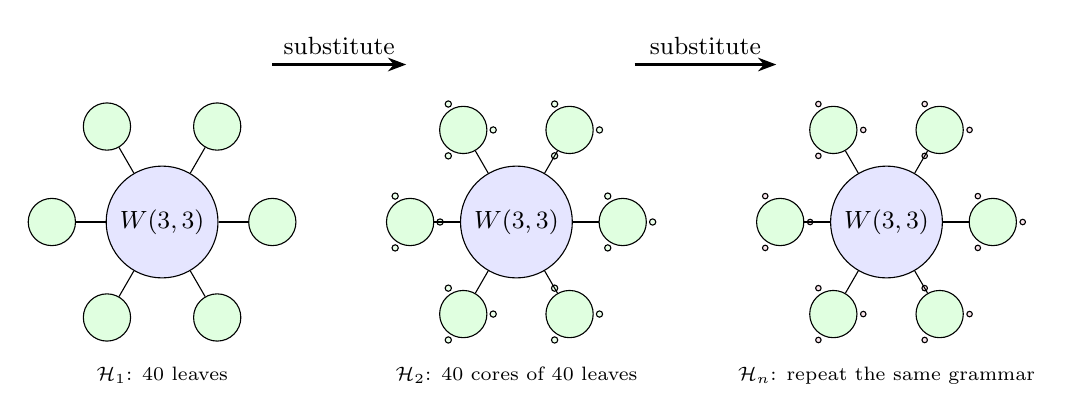
\begin{tikzpicture}[
  every node/.style={font=\small},
  core/.style={circle,draw,fill=blue!10,minimum size=9mm},
  sub/.style={circle,draw,fill=green!12,minimum size=6mm},
  arrow/.style={-{Stealth},thick}
]
  \node[core] (h1) at (0,0) {$\W$};
  \node[font=\scriptsize,fill=white,inner sep=1pt] at (0,-1.95) {$\mathcal{H}_1$: 40 leaves};
  \foreach \i in {0,...,5}{
    \node[sub] (a\i) at ({60*\i}:1.4) {};
    \draw (h1) -- (a\i);
  }
  \node[core] (h2) at (4.5,0) {$\W$};
  \foreach \i in {0,...,5}{
    \node[sub] (b\i) at ($(h2)+({60*\i}:1.35)$) {};
    \foreach \j in {0,1,2}{
      \node[circle,draw,fill=green!8,inner sep=0.8pt]
        at ($(b\i)+({120*\j}:0.38)$) {};
    }
    \draw (h2) -- (b\i);
  }
  \node[font=\scriptsize,fill=white,inner sep=1pt] at (4.5,-1.95) {$\mathcal{H}_2$: 40 cores of 40 leaves};
  \node[core] (h3) at (9.2,0) {$\W$};
  \foreach \i in {0,...,5}{
    \node[sub] (c\i) at ($(h3)+({60*\i}:1.35)$) {};
    \foreach \j in {0,1,2}{
      \node[circle,draw,fill=purple!10,inner sep=0.7pt]
        at ($(c\i)+({120*\j}:0.38)$) {};
    }
    \draw (h3) -- (c\i);
  }
  \node[font=\scriptsize,fill=white,inner sep=1pt] at (9.2,-1.95) {$\mathcal{H}_n$: repeat the same grammar};
  \draw[arrow] (1.4,2.0) -- node[above]{substitute} (3.1,2.0);
  \draw[arrow] (6.0,2.0) -- node[above]{substitute} (7.8,2.0);
\end{tikzpicture}
\caption{Fractal scaling schematic.  The drawn fans show only a few
children; the rule is exact substitution of forty child holonets at
each substrate point.  Routing grows logarithmically in the number of
photonic leaves because each recursive digit costs at most eight
reversible moves.}
\end{figure}

This resolves the computer-engineering question.  A conventional
machine grows by adding processors connected by a separate network.
The holonet grows by adding copies of the same object; each copy
contains its own processor, router, memory, clock, and packet format.
There is no von Neumann bus to saturate.  At every scale, the edge set
is both communication bandwidth and entangling-gate availability, the
chart atlas is both routing table and instruction decoder, and the
Steinberg $81$-sector is both protected memory and fault-tolerant
logical space.

%======================================================================
\section{Runtime closure: compile, monitor, commit}
\label{sec:runtimeclosure}

The architecture now has an executable operating-system loop.
\[
\hbox{address word}\ \longrightarrow\
\hbox{packet route}\ \longrightarrow\
\hbox{sentinel monitor}\ \longrightarrow\
\hbox{durable tomotope commit}.
\]
BT828--BT831 make each arrow finite and testable.

\begin{theorem}[BT828 packet compiler]
A recursive address word with digits in $\{0,\ldots,39\}$ compiles to
a sequence of digit packets
\[
(Q_3\hbox{-XOR hops},\ \hbox{apartment hops},\ D_{12}\hbox{ mirror slot},
\ C_{12}\hbox{ phase},\ \hbox{tomotope block}).
\]
Each digit uses at most three XOR hops and at most five apartment hops,
hence at most eight reversible moves.  The stress route
\[
(0,7,14,21,28,35)\longrightarrow(39,32,25,18,11,4)
\]
compiles to $47$ reversible moves, below the level-six bound $48$.
\emph{Witness: \path{bt828_holonet_packet_compiler.py}.}
\end{theorem}

\begin{theorem}[BT829 sentinel monitor]
The projector onto the $g=15$ adjacency sector of $\W$ has exact
entry profile
\[
P_{-4}(x,x)=\frac38,\qquad
P_{-4}(x,y)=
\begin{cases}
-\frac18,&x\sim y,\\[2pt]
\frac1{24},&x\nsim y.
\end{cases}
\]
Consequently a full context line $K_4$ is sentinel-invisible, while
localized, mirror, and shell faults activate the sentinel with exact
energies:
\[
\begin{array}{c|c|c}
\hbox{fault} & \hbox{energy} & \hbox{normalized fraction}\\
\hline
\hbox{single point} & 3/8 & 5/13\\
\hbox{adjacent edge} & 1/2 & 5/19\\
\hbox{nonedge mirror pair} & 5/6 & 25/57\\
\hbox{gauge shell }N(x) & 6 & 5/7\\
\hbox{matter shell} & 27/8 & 5/13
\end{array}
\]
The immune system is therefore not generic noise detection: it is
blind to legal context-line traffic and tuned to off-context routing
and shell congestion.
\emph{Witness: \path{bt829_fault_sentinel_monitor.py}.}
\end{theorem}

\begin{theorem}[BT830 two-phase commit clock]
The runtime has two clocks.  The reversible prepare phase finishes in
at most $8n$ moves.  The durable commit phase waits for
\[
T(n)=4(7^n-1).
\]
For $1\le n\le24$, $T(n)$ is always divisible by $24$ and by $8$,
so it is aligned with both the local runtime stabilizer and the
single-digit route window.  But it is not always divisible by the full
$8n$ route epoch: the first desynchronization is $n=5$, with remainder
$24=f$.  Thus the commit layer is deliberately slower and cover-like;
it is not merely the route clock renamed.
\emph{Witness: \path{bt830_two_phase_commit_clock.py}.}
\end{theorem}

\subsection{The infinite-cover warning}

The tomotope contributes a harder boundary than the earlier packet
picture showed.  Monson, Pellicer, and Williams prove that the
tomotope has infinitely many distinct minimal regular covers; for
coprime odd $p,q>1$ there are minimal covers $R_p,R_q$ of the
tomotope such that neither covers the other, and neither covers the
special $R_2$ cover \cite{tomotope}.  They also record the toroidal
cover arithmetic
\[
|{\rm Mon}(Q_k)|=36864\,k^6,\qquad
Q_k:\ (4,24,32,8,4)k^3
\]
for vertices, edges, triangles, tetrahedra, and octahedra.

Architecturally this is a big correction.  The $48$-block tomotope
middle layer is a stable local ABI, but the global regular cover is
not unique.  Durable storage must therefore carry a \emph{cover
index} $k$ as an implementation gauge.  Fast routes compile to the
same invariant packet, while persistent storage may choose one minimal
cover family without invalidating the other non-comparable families.
\emph{Witness: \path{bt831_tomotope_minimal_cover_architecture.py}.}

\subsection{Cover-indexed storage, rerouting, and guard bands}

The infinite-cover warning would be useless as engineering unless it
changed the runtime.  BT832--BT834 make it operational.  The principle
is that the local tomotope packet is the ABI and the chosen regular
cover is the storage backend.

\begin{theorem}[BT832 cover-indexed durable storage]
For every supported cover index $k$, durable storage is the lifted
packet space
\[
\{0,\ldots,47\}\times \mathbb{Z}_k^3,
\qquad
|\hbox{slots}|=48k^3,
\]
with projection back to the fast-route ABI by forgetting the
$\mathbb{Z}_k^3$ coordinate.  The kernel to the base tomotope packet has
order
\[
k^6=(k^3)^2,
\]
matching the Monson--Pellicer--Williams toroidal cover law
$|{\rm Mon}(Q_k)|=36864k^6$.  Changing $k$ changes durable capacity and
kernel size, but not the packet program seen by the compiler.  Tested
cover gauges $k=3,5,7,11,13$ all reduce exactly to the same $48$-block
ABI, and larger $k$ reduces the load fraction of the same stress
program.
\emph{Witness: \path{bt832_cover_indexed_durable_storage.py}.}
\end{theorem}

\begin{theorem}[BT833 sentinel-aware packet rerouting]
The BT829 projector supplies a compiler-visible cost function.  Before
the durable commit, each digit route may insert up to two W33 waypoint
points and minimize
\[
\hbox{sentinel energy first, reversible move count second}.
\]
The extra reversible moves are charged to the slower BT830 commit
phase, not to the BT827 fast $8n$ route bound.  In the level-six stress
program the direct route uses $47$ moves and total sentinel energy $4$;
the sentinel-aware route uses $58$ moves, still far below the
$470592$-tick commit window, and lowers the total sentinel energy to
$2$.  Each tested digit route strictly lowers its own $g=15$ energy;
adjacent endpoints can be context-completed to zero, and nonedge mirror
pairs drop below their direct $5/6$ activation.
\emph{Witness: \path{bt833_sentinel_aware_packet_rerouter.py}.}
\end{theorem}

\begin{theorem}[BT834 desynchronization guard-band arithmetic]
The two-phase clock has an exact number-theoretic boundary.  Full
route-epoch synchronization is
\[
8n\mid T(n)=4(7^n-1),
\]
equivalently
\[
2n\mid 7^n-1.
\]
For every odd prime power $p^a\mid n$ with $p\ne7$, this requires
$\operatorname{ord}_{p^a}(7)\mid n$; if $7\mid n$, synchronization is
impossible because the base is not coprime.  The first failure is
$n=5$: $\operatorname{ord}_5(7)=4\nmid5$, and the remainder is
\[
T(5)\bmod 40=24=f.
\]
Thus the first cover-index where durable storage and the full route
epoch separate is not empirical drift; it is the $f=24$ guard band of
the tomotope-backed runtime.
\emph{Witness: \path{bt834_desync_guard_band_arithmetic.py}.}
\end{theorem}

\begin{theorem}[BT838 tomotope Wythoff runtime ladder]
The Gr\"unbaum--Coxeter/tomotope operation tables give the local
tomotope counts
\[
\hbox{original},\ \hbox{rectified},\ \hbox{truncated},\
\hbox{maximal expanded},\ \hbox{omnitruncated}
\quad=\quad
4,\ 12,\ 24,\ 48,\ 96.
\]
These are exactly the runtime packet-growth layers:
\[
4=\mu\quad(\hbox{vertex carriers}),\qquad
12=k\quad(\hbox{edge axes}),\qquad
24=f\quad(\hbox{$D_{12}$ lift}),
\]
\[
48=2f\quad(\hbox{BT814 packet ABI}),\qquad
96=4f\quad(\hbox{half-flag boundary}).
\]
The doubled omnitruncated boundary gives the verified full packet
flags, $2\cdot96=192$.  After a cover lift this becomes
\[
48k^3=\hbox{BT832 lifted packet capacity},\qquad
192k^3=|W_k|,
\]
the $W_k$ order already recorded in the tomotope cover architecture.
Thus the Wythoff operations are not decorative variants; they are the
compiler's packet expansion states:
\[
\hbox{carrier}\to\hbox{edge-axis}\to\hbox{mirror lift}
\to\hbox{packet ABI}\to\hbox{flag boundary}.
\]
\emph{Witness: \path{bt838_tomotope_wythoff_runtime_ladder.py}.}
\end{theorem}

%======================================================================
\section[The fuel: matter equals magic]{The fuel: matter $=$ magic}
\label{sec:fuel}

\begin{theorem}[The triality]
In the photon's two-qubit reading, exactly the $4$ basis rays are
stabilizer states and all $36$ $\omega$-rays are magic (no stabilizer
state has support $3$).  Consequently three classifications coincide
exactly, on rays $[4,36]$ and on contexts $\{4{:}1,\,1{:}12,\,0{:}27\}$:
the holonet vacuum split, the Schmidt (self-entanglement) strata, and
the magic strata.  \emph{The matter shell is the machine's
non-classical resource sector.}
\emph{Witness: \texttt{bt822}.}
\end{theorem}

\begin{theorem}[Three grades and the cube inside]
Stabilizer fidelity splits the $36$ magic rays into grades
\[
\underbrace{8}_{2^q}\ \text{deep}\ \Bigl(F=\tfrac{2+\sqrt3}{6}\Bigr),
\qquad
\underbrace{24}_{f}\ \text{mid}\ \Bigl(F=\tfrac{5+2\sqrt3}{12}\Bigr),
\qquad
\underbrace{4}_{\mu}\ \text{shallow}\ \Bigl(F=\tfrac34=\tfrac q\mu\Bigr),
\]
the shallow grade sitting exactly at the Werner decoherence threshold.
The $8$ deep rays are precisely the point set of a hyperbolic polar
pair (the $24$-cell vacuum axis), and the $27$ fully-magic contexts
stratify by grade signature as $1+8+12+6$ --- the cell census of the
cube.  \emph{Witnesses: \texttt{bt822}, \texttt{bt823}.}
\end{theorem}

\begin{theorem}[Exact contextuality budget]
The maximum number of contexts a classical $\{0,1\}$ valuation can
satisfy exactly-once is exactly $36=(q!)^2$ (complete branch-and-bound
over all $2^{40}$ markings): classicality saturates at the spread
count, the deficit is exactly $\mu=4$, and the contextual fraction is
exactly $1/10=1/\Phi_4$.  A perfect valuation would be an ovoid, and
$\W$ has none: the true independence number is $\alpha=7=\Phi_6$,
attained only by the beacon heptads of \S\ref{sec:sync}, against the
Lov\'asz bound $\vartheta=10$ --- the $\vartheta-\alpha$ gap $3=q$ is
the combinatorial face of Kochen--Specker.
\emph{Witnesses: \texttt{bt818}, \texttt{bt823}.}
\end{theorem}

\begin{theorem}[Conditional matter-equals-magic architecture]
The exact finite inputs are the $36=(q!)^2$ distinguished rays, their
$8+24+4=\{2^q,f,\mu\}$ grading, the contextual fraction
$1/\Phi_4=1/10$, and the qutrit Strange state's mana $\log(5/3)$
(stabilizer states have mana $0$).  Separately, the homological register is
the $[[240,81,3]]_3$ Steinberg code, equivalently
$[[240,81,4,3]]_3$ in the ordered convention $[[n,k,d_Z,d_X]]_3$.
If a protected encoding and injection map identifies prepared copies of the
distillable state with the distinguished-ray sector of that register, then
one hardware layer could serve both error correction and non-Clifford
injection.  The counts and contextuality witness do not construct that map,
prove replenishment, or remove a distillation factory.
\emph{Witness: \path{analysis/w33_magic_economy.py}.}
\end{theorem}

\paragraph{Exact resource boundary from the QR branch (Passes 361--367).}
The theorem above is an architectural proposal for the qutrit/GKP branch; a
count of contextual rays is not by itself a compiled injection circuit or a
threshold theorem.  The independently certified binary QR-137 branch makes
that distinction concrete.  Its one-block simple lift supplies only logical
$H$; the multi-block construction supplies the real Clifford tower
$O^+(2m,2)$; and the first named phase lift is the weight-$137$ Clifford
rotation $\exp(-\pi i\bar Z/4)$.  That operator normalizes the exact
stabilizer but is not yet transversal, local, low-weight, or proved
fault-tolerant.  Consequently the QR witnesses do not establish $P=1$ or
remove magic-state distillation.  Doing so requires an explicit protected
resource-state preparation/injection circuit, decoder, and noise-threshold
analysis for the chosen physical branch.

\paragraph{The conditional resource accounting.} Define
the non-Clifford premium $P=\mathrm{cost}(\text{non-Clifford})/\mathrm{cost}(\text{Clifford})$.
In the surface-code baseline a non-Clifford gate needs a distilled magic state, so
$P\sim O(d^3)$ (the distillation factory, $\sim10^3$--$10^4$ qubit-rounds at useful code
distances $d$, occupying $30$--$90\%$ of the device --- the dominant cost of fault
tolerance).  In the proposed shared-layer implementation, $P=1$ is a design
target: it would require a protected injection to cost one correction cycle.
Neither the equality nor an $O(d^3)$ saving follows until that injection,
decoder, and threshold are supplied. (Witness:
\path{analysis/w33_magic_resource_accounting.py}.)

\paragraph{What the irrational clock does and does not prove.} The Boerdijk--Coxeter twist
$\theta=\arccos(-2/3)$ --- the $q=3$ simplex angle, $-2/3=-(q-1)/q$ --- has $\theta/\pi$
\emph{irrational} (Niven, since $\cos\theta=-2/3\notin\{0,\pm\tfrac12,\pm1\}$), so the
stroboscopic phases $\{n\theta\bmod2\pi\}$ never repeat, are Weyl-equidistributed (star
discrepancy $\to0$), obey the Steinhaus three-gap law, and never land exactly on a
stabilizer angle $2\pi k/q$.  This proves aperiodicity, not gate type:
an irrational phase sequence need not implement a cubic Hamiltonian, a
distillable state, or a protected non-Clifford injection.  Establishing
replenishment requires an explicit driven Hamiltonian/control map and a
classification of its logical action. (Witness:
\path{analysis/w33_clock_magic_renewal.py}.)

\paragraph{And the code is holographic.} The matter shell is not just a code but a
\emph{holographic} one. From any pole the $40$ rays split $1+12+27=$ self $+$ gauge
boundary $+$ matter bulk, and every bulk ray is screened by exactly $\mu=4$ boundary
rays.  That strongly-regular screening multiplicity is a combinatorial redundancy,
not the full CSS distance: the edge code has $d_X=3$, $d_Z=4$, and hence $d=3$.
It therefore corrects one arbitrary qutrit error or two known-location arbitrary
erasures.  The $\mu=4$ neighbourhood by itself does not prove recovery from three
arbitrary erasures; an operational bulk-reconstruction map would be additional data. The causal
diameter is $2$ (every bulk ray one hop from the boundary, two from the pole), the
RT-like depth; and the logical register $H_1$ is the irreducible Steinberg module
(dim $81=q^4$), so there is no local logical operator --- logical information lives only
nonlocally on the boundary. Boundary redundancy, an RT-like causal depth, and no local
logical representative are the proposed holographic signature:
the ``holo'' in holonet is earned. (Witness:
\path{analysis/w33_holographic_code.py}.)

\begin{theorem}[Conditional self-fueling holographic-memory proposal]
The exact finite inputs are the Steinberg-code dimensions and distances
$(k,d_X,d_Z)=(81,3,4)$, screening multiplicity $\mu=4$, the
$36$-ray contextual sector, the fraction $1/10$, the irrational angle
$\arccos(-2/3)$, and the graph-cut counts $12$, $4$, and
$108=4\cdot27$.  Calling these one self-fueling holographic memory requires
three additional maps: a bulk--boundary recovery channel, a protected
resource-state injection, and a logical clock action that actually produces
that resource.  The current witnesses certify the finite inputs, not those
identifications; in particular they do not prove $P=1$ or eliminate
distillation. (Witnesses: \path{analysis/w33_self_fueling_memory.py},
\path{analysis/w33_holographic_rt.py}.)
\end{theorem}

\begin{theorem}[Finite-curvature/de Sitter analogy and conditional cost model]
The collinearity graph $\W$ has positive Ollivier--Ricci curvature ---
computed by optimal transport, $\kappa=1-W_1(m_x,m_y)=1/6=2/k$ --- the discrete
finite identity $E\,\kappa=240\cdot\tfrac16=40=v$ (Face~1). These exact
facts motivate a de Sitter analogy; they do not identify the graph with
spacetime, its cuts with horizons, or its clock with cosmological time.
(Witness:
\path{analysis/w33_memory_is_desitter.py}.)

\emph{Conditional cost model.} If the missing protected injection consumes
resource states at the contextual-fraction rate $1/\Phi_4=1/10$ per cycle,
then a circuit with non-Clifford fraction $f\le1/10$ would avoid rate
throttling, while $f>1/10$ would require the model factor $10f$ in time or
parallel cores.  The finite fraction is exact; the replenishment law, factory
removal, and claimed hardware saving remain conditional on the unbuilt
compiler and threshold. (Witness: \path{analysis/w33_self_fueling_cost.py}.)
\end{theorem}

%======================================================================
\section{Memory, protection, and the immune system}
\label{sec:memory}

\begin{theorem}[The code register is the Steinberg module]
The companion paper's CSS code $[[240,81,3]]_3$, with asymmetric distances
$(d_X,d_Z)=(3,4)$, stores its $81$
logical qutrits in $H_1$ of the $\W$ $2$-complex ($40$ vertices,
$240$ edges, $160$ in-line triangles).  Complete character
computation over all $25920$ group elements gives
\[
\langle\chi_{H_1},\chi_{H_1}\rangle=1.
\]
Therefore $H_1\otimes\mathbb{C}$ is
\emph{irreducible} of dimension $81$, hence equal to the unique
$81$-dimensional irreducible --- \textbf{the Steinberg module} ---
with $\chi_{H_1}(g)=\#\mathrm{fixflags}-\#\mathrm{fixpoints}
-\#\mathrm{fixlines}+1$ (the Solomon--Tits alternating sum) verified
for every $g$.  The QECC logical space and the Schur-protected
register below are one object: any equivariant logical error is a
scalar, so only symmetry-breaking noise can touch the code, and the
sentinel/clock layers are exactly the symmetry monitors.  The
homological dictionary then completes: $H_0$ is trivial (the vacuum
pole), $H_1$ is Steinberg (the register), and $H_2$ (dim $40$, one
tetrahedron-boundary $2$-cycle per line) is the \emph{sign-twisted}
line module --- a fixing symmetry acts on a line's $2$-cycle by the
parity of its induced $S_4$ action (verified for all $25920$
elements; \emph{not} the plain permutation module): the top homology
is the \emph{oriented} timetable carrier, feeding the chirality
ledger.
\emph{Witnesses: \texttt{bt861\_code\_register\_is\_steinberg.py},
\texttt{bt862\_h2\_is\_the\_line\_module.py}.}
\end{theorem}

\begin{corollary}[Three generations from Steinberg vanishing]
$\chi_{\mathrm{St}}(g)=0$ iff $3\mid\mathrm{ord}(g)$ (verified for
all $25920$ elements).  Hence \emph{any} order-$3$ symmetry of the
substrate splits the matter register into eigenspaces of exactly
$27+27+27$ --- the three-generation decomposition is forced for
every choice of triality element, not selected --- and every
order-$9$ element ($5760$ of them) refines it into nine
$9$-dimensional sub-generations.  In the code's own characteristic
the parameters survive: $\mathrm{rank}_3\partial_0=39$,
$\mathrm{rank}_3\partial_1=120$, $\dim H_1(\GF3)=81$, so the logical
dimension of $[[240,81,3]]_3$ is exact over $\GF3$.  The number of fermion
generations is the defining-characteristic degeneracy of the
protected register.
\emph{Witness:
\texttt{bt863\_generations\_from\_steinberg\_vanishing.py}.}
\end{corollary}

\begin{theorem}[The dual-torsor Steinberg compiler]
Let $H_{27}=3^{1+2}_{+}$ be the canonical Heisenberg $O_3$ of the
point parabolic and let $A_{27}=\GF3^3$ be the canonical translation
$O_3$ of the Bell-line parabolic.  Their $27$-point and $27$-line
shells are regular torsors (BT858).  On the protected register,
\[
 \mathrm{St}\!\downarrow_{H_{27}}=3\,\mathbb{C}[H_{27}],
 \qquad
 \mathrm{St}\!\downarrow_{A_{27}}=3\,\mathbb{C}[A_{27}],
\]
because both restricted characters are exactly
$\{81^1,0^{26}\}$.  The statement survives in the code's own field
and is constructive:
\[
 H_1(\W;\GF3)\!\downarrow_{H_{27}}
   \cong \GF3[H_{27}]^{\oplus3},
 \qquad
 H_1(\W;\GF3)\!\downarrow_{A_{27}}
   \cong \GF3[A_{27}]^{\oplus3}.
\]
For each torsor the verifier finds three cycle seeds whose $27$ group
translates add $27+27+27$ independent classes modulo the
$120$-dimensional boundary space.  Thus the same logical memory has a
flat program basis and a curved state basis: $A_{27}$ is the
commuting three-trit address compiler, while $H_{27}$ is the
noncommuting qutrit-phase compiler.

The center $Z(H_{27})=\langle z\rangle\cong C_3$ selects a canonical
triality.  Over $\mathbb{C}$ its central-character blocks are
\[
 H_1=H_{1,1}\oplus H_{1,\omega}\oplus H_{1,\omega^2},
 \qquad \dim H_{1,j}=27.
\]
The trivial block contains the nine linear characters with
multiplicity $3$; the two nontrivial blocks contain the conjugate
$3$-dimensional Schr\"odinger representations with multiplicity $9$.
Over $\GF3$, where $x^3-1=(x-1)^3$, the phases coalesce into a
canonical unipotent flag.  With $N=z-I$,
\[
 (\operatorname{rank}N,\operatorname{rank}N^2,
   \operatorname{rank}N^3)=(54,27,0),
\]
so
\[
 0\subset\ker N\subset\ker N^2\subset H_1,
 \qquad \dim=(0,27,54,81),
\]
has three successive quotients of dimension $27$.  Equivalently,
$z$ acts by $27$ Jordan blocks of length $3$.  Complex generations
are phase sectors; native qutrit generations are the three layers of
one depth-$3$ memory stack.

The freeness is canonical, but the displayed orbit bases are not:
$H_{27}$ and $A_{27}$ are nonisomorphic, and a basis-to-basis matrix
still requires a chosen point, line, shell origin, and cycle seeds.
No canonical intertwiner is claimed.
\emph{Witness:
\texttt{bt865\_dual\_torsor\_steinberg\_compiler.py}.}
\end{theorem}

\begin{figure}[ht]
\centering
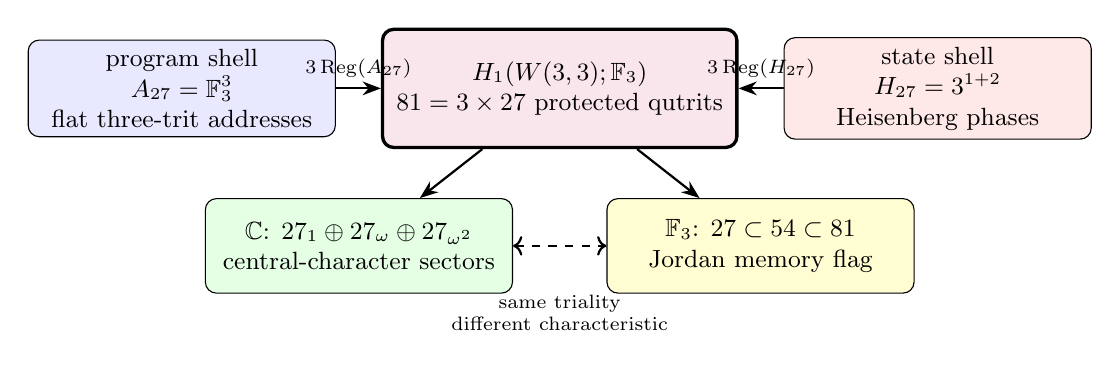
\begin{tikzpicture}[
  box/.style={draw,rounded corners,align=center,minimum width=39mm,
              minimum height=12mm,font=\small},
  core/.style={draw,very thick,rounded corners,align=center,
               minimum width=45mm,minimum height=15mm,font=\small},
  arrow/.style={-{Stealth},thick}
]
  \node[box,fill=blue!9] (program) at (-4.8,0)
    {program shell\\$A_{27}=\GF3^3$\\flat three-trit addresses};
  \node[core,fill=purple!10] (memory) at (0,0)
    {$H_1(\W;\GF3)$\\$81=3\times27$ protected qutrits};
  \node[box,fill=red!9] (state) at (4.8,0)
    {state shell\\$H_{27}=3^{1+2}$\\Heisenberg phases};
  \node[box,fill=green!10] (complex) at (-2.55,-2.0)
    {$\mathbb C$: $27_1\oplus27_\omega\oplus27_{\omega^2}$\\
     central-character sectors};
  \node[box,fill=yellow!18] (native) at (2.55,-2.0)
    {$\GF3$: $27\subset54\subset81$\\Jordan memory flag};
  \draw[arrow] (program) -- node[above,font=\scriptsize]
    {$3\,\mathrm{Reg}(A_{27})$} (memory);
  \draw[arrow] (state) -- node[above,font=\scriptsize]
    {$3\,\mathrm{Reg}(H_{27})$} (memory);
  \draw[arrow] (memory) -- (complex);
  \draw[arrow] (memory) -- (native);
  \draw[<->,thick,dashed] (complex.east) -- (native.west);
  \node[font=\scriptsize,align=center] at (0,-2.85)
    {same triality\\different characteristic};
\end{tikzpicture}
\caption{The dual-torsor compiler.  Flat program translations and
noncommutative state translations give two free rank-$3$ module
coordinates on one Steinberg-protected register.  The Heisenberg
center reads as three phase sectors over $\mathbb C$ and as a
three-step unipotent memory flag over $\GF3$.}
\label{fig:dual-torsor-compiler}
\end{figure}

\begin{theorem}[Steinberg memory]
The Levi-graph cycle space and the chart-overlap $81$-sector are both
irreducible and equal to the Steinberg representation of
$\PSp(4,3)$ --- the Solomon--Tits homology of the building, whose
canonical basis is the $81$ apartments through any chamber.  Schur's
lemma then forces the uniqueness of the chart--cycle bridge.  Restricted
to a Sylow $3$-subgroup the module is free of rank one: the protected
memory is one free generator over the substrate's ternary symmetry.
\emph{Witnesses: \texttt{bt742}, \texttt{bt744}.}
\end{theorem}

\begin{corollary}[The oriented timetable spectrum]
Let $P=3^3{:}S_4$ be the index-$40$ line parabolic.  The ordinary
line permutation module and the oriented top-homology module are the
two inductions of its two linear characters:
\[
 \operatorname{Ind}_P^{\PSp(4,3)}(1)=1\oplus15\oplus24,
 \qquad
 H_2=\operatorname{Ind}_P^{\PSp(4,3)}(\operatorname{sign}_{S_4})
   =5_{\omega}\oplus5_{\omega^2}\oplus30.
\]
The two 5-dimensional characters are complex conjugates over
$\mathbb Q(\zeta_3)$; the 30 is rational.  Under the outer extension
$W(E_6)=U_4(2){:}2$, the conjugate pair is the restriction of one
irreducible 10-dimensional representation, whereas the 30 has two
inequivalent extensions.  Thus the oriented timetable header reads
as a Weyl-visible chiral channel $10$ plus a payload $30^{\pm}$ whose
outer parity is not fixed by the projective module alone.

The completed homology spectrum is
\[
 H_0=1,\qquad H_1=\mathrm{St}_{81},\qquad
 H_2=5_{\omega}\oplus5_{\omega^2}\oplus30,
\]
and resolves the Euler charge representation by representation:
\[
 1-81+(5+5+30)=-40=-v.
\]
BT867 resolves the tempting cache comparison negatively: neither
$162$-cache branch is one of the two 5-dimensional sectors.  The
branches are isomorphic copies with identical character overlaps; the
outer involution acts on their multiplicity label.  The possible
identification of the two 30-extensions with BT857's local gauge bit
remains open.
\emph{Witness:
\path{analysis/bt866_h2_oriented_irreducible_decomposition.py}.}
\end{corollary}

\begin{theorem}[The cache/transport extension boundary]
\label{thm:cache-transport-boundary}
Let $H=3^3{:}S_4$ be the order-$648$ Bell-line parabolic.  The two
$162$-slot BT859 cache branches have conjugate cyclic stabilizers and
are therefore isomorphic transitive $H$-sets,
\[
  \mathcal C_L\cong H/C_4\cong\mathcal C_R.
\]
Their permutation characters are equal.  In particular, their scalar
products with the restrictions of the three BT866 characters
$(5_\omega,5_{\omega^2},30)$ are both $(1,1,8)$: each cache sees both
conjugate 5-sectors equally.  ``Left'' and ``right'' are copy labels,
not internal spectral chiralities.

The parabolic contains one conjugacy class of $81$ cyclic $C_4$
subgroups, and
\[
 N_H(C_4)=D_8,
 \qquad
 H/C_4\longrightarrow H/D_8,
 \qquad
 162\longrightarrow81
\]
is the canonical free two-sheet cache cover.  Both copies cover this
same stabilizer base.  On their union GAP computes
\[
 C_{\operatorname{Sym}(324)}(H)\cong D_8,
 \qquad
 324=81\times4=81\times2_{\rm deck}\times2_{\rm cache},
\]
with exactly $81$ commutant orbits of size four.  Thus the four-state
fiber carries the symmetry of a square, not merely a numerical pair of
bits.

This cache carrier is not the older ternary $162$-sector.  On one
cache fiber the deck swap and its two projectors are
\[
 D=\begin{pmatrix}0&1\\1&0\end{pmatrix},
 \qquad
 P_\pm=\frac{I\pm D}{2},
 \qquad
 \GF3^2=\operatorname{im}P_+\oplus\operatorname{im}P_-.
\]
Since $2$ is invertible in $\GF3$, the cache splits; indeed
$(D-I)^2=D-I$.  By contrast, packet transport uses
\[
 N=\begin{pmatrix}0&1\\0&0\end{pmatrix},
 \qquad N^2=0,
 \qquad (I+N)^3=I,
\]
and tensors this indecomposable fiber with the $81$-register to obtain
the non-split sequence $0\to81\to162\to81\to0$.  No change of basis
can identify the idempotent cache difference with the nilpotent
transport shift.  The architecture therefore separates a reversible
\emph{address/control plane} from a memory-bearing ternary
\emph{temporal data plane} by extension class, not by convention.
\emph{Witness:
\path{analysis/bt867_cache_split_transport_nonsplit_boundary.py}.}
\end{theorem}

\begin{figure}[ht]\centering
\resizebox{0.98\textwidth}{!}{%
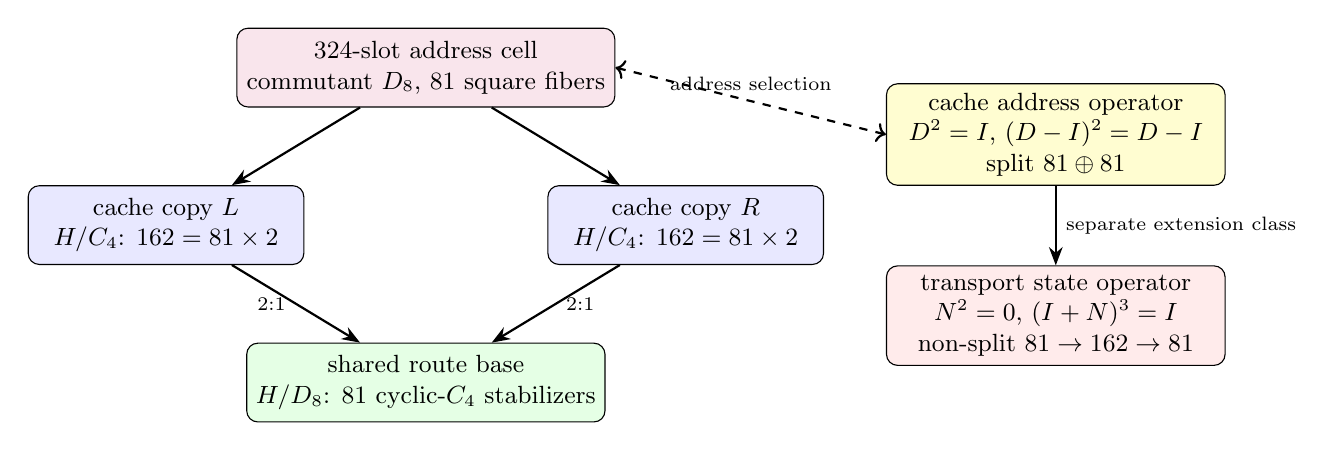
\begin{tikzpicture}[
  every node/.style={font=\small},
  box/.style={draw,rounded corners,align=center,minimum width=35mm,minimum height=10mm},
  arr/.style={-{Stealth},thick}
]
  \node[box,fill=green!10] (base) at (0,0)
    {shared route base\\$H/D_8$: $81$ cyclic-$C_4$ stabilizers};
  \node[box,fill=blue!9] (left) at (-3.3,2.0)
    {cache copy $L$\\$H/C_4$: $162=81\times2$};
  \node[box,fill=blue!9] (right) at (3.3,2.0)
    {cache copy $R$\\$H/C_4$: $162=81\times2$};
  \node[box,fill=purple!10,minimum width=48mm] (union) at (0,4.0)
    {$324$-slot address cell\\commutant $D_8$, $81$ square fibers};
  \draw[arr] (left) -- node[left,font=\scriptsize] {$2{:}1$} (base);
  \draw[arr] (right) -- node[right,font=\scriptsize] {$2{:}1$} (base);
  \draw[arr] (union) -- (left);
  \draw[arr] (union) -- (right);

  \node[box,fill=yellow!18,minimum width=43mm] (split) at (8.0,3.15)
    {cache address operator\\$D^2=I$, $(D-I)^2=D-I$\\split $81\oplus81$};
  \node[box,fill=red!8,minimum width=43mm] (nonsplit) at (8.0,0.85)
    {transport state operator\\$N^2=0$, $(I+N)^3=I$\\non-split $81\to162\to81$};
  \draw[<->,thick,dashed] (union.east) -- node[above,font=\scriptsize]
    {address selection} (split.west);
  \draw[arr] (split) -- node[right,font=\scriptsize]
    {separate extension class} (nonsplit);
\end{tikzpicture}}
\caption{The local cache cell and the split/non-split boundary.  The
$D_8$ square fiber chooses a reversible address over one of $81$ routes;
the independent ternary nilpotent updates state while retaining temporal
memory.  Equal 162-dimensional counts do not imply equivalent modules.}
\label{fig:cache-transport-boundary}
\end{figure}

The error layer is native: the $[[240,81,3]]_3$ CSS code on the edge
qutrits has $(d_X,d_Z)=(3,4)$; the dual
Cs\'asz\'ar/Szilassi cross-check supplies parity-free error detection;
and the web's unique non-Ramanujan eigenspace --- dimension $15=g$ ---
is the spectral sentinel where drift appears first.  At the classical
boundary-image layer, Pass~373 gives the exact $[240,120,3]_3$ code and a
complete 481-entry radius-one syndrome table, so one edge-symbol fault has a
fully enumerated decoder.  Pass~374 adds a separate controller constraint:
the 51840 nonzero minimal logical $X/Z$ vector pairings occupy four invariant
12960-state sheets under the natural $W(E_6)$ action, with stabilizer
$C_2\times C_2$.  A runtime using those scalar representatives must therefore
retain the two deck-sign bits; geometry does not collapse them to one Weyl
torsor.  Pass~375 sharpens the controller law: the fixed pairing character
reduces the four-state sheet normalizer from abstract $S_4$ to the
phase-compatible $D_8$, with no order-three operation.  The split controller
$W(E_6)\times V_4$ has no regular 51840-state complement.  A future sheet
fusion must therefore be a genuinely coupled transport, not an appended
commuting phase register.

%======================================================================
\section{Time: three clocks and a quasicrystal}
\label{sec:time}

\begin{theorem}[Clock trichotomy]
Of the program's three natural clocks, exactly one is internal:
$\mathbb{Z}_{12}$ (the rectangle clock, $12\mid 51840$) runs the
selector and duo machinery, while $\mathbb{Z}_7$ (Cs\'asz\'ar) and
$\mathbb{Z}_{13}$ (Singer) do not divide the group order and act as
external references --- both with decimal period $6=q!$, so the digit
expansion of $1/7$ is literally the internal clock's shadow modulo its
duo bit.
\emph{Witnesses: \texttt{bt774}, \texttt{bt803}, \texttt{bt807},
\texttt{bt819}.}
\end{theorem}

\begin{theorem}[The Boerdijk--Coxeter time quasicrystal]
Driving the loop by the BC twist $\theta=\arccos(-2/3)$ per round trip
yields a stroboscopic orbit that provably never repeats (Niven), with
the Steinhaus three-distance signature at all substrate step counts and
--- the substrate's signature moment --- exactly \emph{two} gap lengths
at $n=30=h(E_8)$, the BC ring length, where closure happens in $S^3$
(the $600$-cell) rather than the phase circle (deficit $0.0158$).
This is the photonic sibling of the Fibonacci-drive dynamical
topological phase.
\emph{Witness: \texttt{bt820}.}
\end{theorem}

\begin{corollary}[The machine's clock is the universe's clock]
The same BC clock is the de Sitter beat of inflation (Face~7). Its twist
$\cos\theta=-(q-1)/q$ is the discrete de Sitter angle, its ring length is the beat
$30=h(E_8)$ (the $600$-cell's $20$ rings of $30$), and the inflationary cosmology reads
off that beat: the e-fold number is $N=2(v-\Phi_4)=2\,h(E_8)=60$, exactly twice the
beat, and the CMB spectral tilt is
\[
1-n_s \;=\; \tfrac{2}{N} \;=\; \tfrac1{30} \;=\; \tfrac1{h(E_8)} \;=\; \tfrac1{\text{(clock beat)}},
\]
so the deviation of the primordial spectrum from scale invariance is the inverse of the
clock's period. The two structures even match in kind: the clock is a \emph{time
quasicrystal} (nearly periodic, never exact) just as inflation is \emph{quasi--de
Sitter} (nearly exponential, never exact) --- both broken de Sitter by $q=3$, the clock's
aperiodicity being the cosmology's tilt. The architecture's time and the universe's
expansion are one quasicrystal.
\emph{Witness: \path{analysis/w33_clock_cosmology.py}.}
\end{corollary}

\begin{corollary}[A falsifiable clock fingerprint in the CMB]
If the clock couples to the inflaton, its quasiperiodicity imprints a \emph{quasi-periodic}
modulation on the primordial spectrum: peaks at log-period $2\pi/\theta\approx2.73$ in
$\ln k$ (with $\theta=\arccos(-2/3)$) whose spacings obey the Steinhaus \emph{three-gap}
law (two gap lengths near the BC ring $n=30$) --- the time-quasicrystal fingerprint,
distinct from smooth slow roll (no peaks) and from single-frequency resonant inflation (a
uniform comb, one gap). The log-frequency and the three-gap shape are fixed by $q=3$; only
the amplitude (the coupling) is free. A CMB feature search (Planck, LiteBIRD, CMB-S4) can
detect the three-gap comb, bound the coupling, or --- finding a clean single-frequency
comb --- disfavour the clock. (Witness:
\path{analysis/w33_cmb_clock_signature.py}.)
\end{corollary}

\begin{theorem}[The arrow of time]
Without its two-trit feedforward record, the photon's
self-configuration loop is the completely depolarizing channel with
unique fixed point $I/q$ --- exactly the Bell marginal; with the
record it is unitary.  Decoherence is self-forgetting, priced at
$\log_3 q^2 = 2$ trits per cycle.
\emph{Witness: \texttt{bt823}.}
\end{theorem}

%======================================================================
\section{Synchronization: beacons and schedules}
\label{sec:sync}

The maximum classically coherent constellations are the
\emph{beacon heptads}: seven states with all pairwise overlaps exactly
$1/3=1/q$ --- a complete $K_7$ interference mesh, the Cs\'asz\'ar
toroidal node realized in light.  There are exactly $2880$ heptads in
a single transitive family; each has a $\mathbb{Z}_3\times\mathbb{Z}_3$
symmetry fixing a unique \emph{master beacon} and cycling two triads
($7=1+3+3$), and single-beacon swaps connect the family into its own
exchange network: the reference frames of the network form a network.
The measurement timetable is rigid: there exist exactly $36$ complete
schedules (partitions of the $40$ states into $10$ contexts) --- an
exhaustive result that simultaneously proves every spread of $\W$ is
regular --- with each context appearing in exactly $9$ schedules.
\emph{Witnesses: \texttt{bt817}, \texttt{bt819}.}

\begin{theorem}[Schedule-overlap law]
Two distinct schedules share exactly $1$ or exactly $4=\mu$ contexts:
each schedule has $15$ \emph{near} partners (overlap $4$) and $20$
\emph{far} partners (overlap $1$), the two relation classes of the
double-six diagonal $[1,15,20]$, with the exact counting identity
$1\cdot 20 + 4\cdot 15 = 80 = 10\times(9-1)$.  Operationally: a cheap
timetable switch preserves $4$ of $10$ calibrated contexts and a far
switch only $1$, so a controller hopping among near partners
re-calibrates $6$ contexts per hop --- the timetable library is itself
a metric space whose geometry is the double-six relation.
\emph{Witness: \texttt{bt835\_schedule\_overlap\_theorem.py}.}
\end{theorem}

\paragraph{The Gr\"unbaum--Coxeter cells.}
Each schedule also has an internal shape.  The full schedule
stabilizer $S_6$ is $2$-homogeneous on the $10$ contexts, but its
icosahedral core $A_5$ --- the $600$-cell level of the platonic
ladder, and \emph{exactly} the automorphism group of the
hemi-dodecahedron $\{5,3\}_5$ --- splits the $\binom{10}{2}=45$
context pairs as $45=15+30$, and the $15$-orbit graph on the $10$
contexts is the \textbf{Petersen graph}: the edge skeleton of the
hemi-dodecahedron, the cell of Coxeter's exceptional $57$-cell.
Dually, the hidden $6$-set of the $S_6$ action realizes the
hemi-icosahedron $\{3,5\}_5$ --- the cell of Gr\"unbaum's $11$-cell
--- with incidence count $(6,15,10)$: six hidden points, fifteen
duads, ten triple-splits $=$ the contexts themselves.  The exceptional
polytopes' groups do not embed in $\Sp(4,\GF3)$, but they are
substrate arithmetic
($|\mathrm{PSL}(2,11)|=660=k\cdot N_{\mathrm{eff}}$,
$|\mathrm{PSL}(2,19)|=3420=k\cdot g\cdot 19$, Heawood genus
$H(19)=20=$ the BC ring count, and $11=k-1$ is the Ihara prime of the
zeta critical circle $|u|=1/\sqrt{11}$): the full $11$-cell and
$57$-cell live elsewhere, yet their \emph{cells} are carried by every
measurement timetable of this machine, glued by the substrate's own
group instead of $\mathrm{PSL}(2,p)$.
\emph{Witness: \texttt{bt836\_gc\_hemicells\_in\_spreads.py}.}

\begin{theorem}[The library is a classical geometry]
\label{thm:library}
The timetable library carries its own rank-3 geometry, and the
hemicell structure fibers over it with perfect uniformity:
(i) every skew line pair lies in exactly $3$ schedules, so the
$(\mathrm{schedule}\supset\mathrm{pair})$ flag count is
$36\times45=1620$ --- the apartment count of the Tits building ---
and $540\times3$;
(ii) the near-partner graph on the $36$ schedules is strongly regular
$\mathrm{SRG}(36,15,6,6)$, the \emph{other} classical rank-3 graph of
$U_4(2)\cong\PSp(4,\GF3)$, so the control plane (timetables) and the
data plane ($\W=\mathrm{SRG}(40,12,2,4)$) are the two rank-3
geometries of one group;
(iii) each schedule stabilizer contains exactly $6$ icosahedral
$A_5$ cores ($216=6^3$ in all, each marking its unique schedule via
its $[10,30]$ line orbits) giving $6$ distinct Petersen splits; each
internal pair is a Petersen edge under exactly $2$ of the $6$ cores,
hence every skew pair of $\W$ has exactly $6=3\times2$
hemi-dodecahedral homes ($3240=540\times6$ Petersen flags).
\emph{Witness: \texttt{bt837\_schedule\_library\_geometry.py}.}
\end{theorem}

\begin{theorem}[Two compasses, twelve Petersens, $4\cdot K_{10}$]
$\PSp(4,\GF3)$ has exactly two conjugacy classes of $A_5$, both with
normalizer $S_5$ and $216$ conjugates, unfused by the outer
automorphism, and \emph{both fiber over the same $36$ schedules}:
every schedule stabilizer contains $12=6+6$ icosahedral cores ---
$6$ \emph{duad} cores (line signature $[10,30]$, the
Theorem-\ref{thm:library}(iii) cores) and $6$ \emph{pentad} cores
(signature $[5,5,10,20]$: transitive on the schedule, plus two
distinguished \emph{pentads} of $5$ pairwise-disjoint lines outside
it).  The two $216$-sets are non-isomorphic $G$-sets (rank $10$
suborbits $[1,5,10,10,20,20,20,30,40,60]$ vs
$[1,5,10,10,20,20,30,30,30,60]$); the Petersen flags form the coset
geometry $\PSp(4,\GF3)/D_4$ ($3240$ flags, dihedral stabilizer).
There are $432$ distinct pentads in \emph{two chiral orbits} of
$216$ (stabilizer order $120$); every core pairs one LEFT with one
RIGHT pentad, and each pentad serves exactly one core.  Pentads are
\emph{maximal partial spreads}: no schedule contains one.  The two
pentads of one core interlock as $K_{5,5}$ minus a perfect matching
--- mutual disjointness is \emph{forbidden} by the overlap law (it
would create a $0$-overlap schedule) --- and the deleted matching
consists of $5$ \emph{skew} pairs, i.e.\ five hypercube charts; over
the $216$ cores these matchings cover the $540$-chart atlas
\textbf{exactly twice} ($1080=540\times2$): the routing fabric is
readable off the pentad compasses, five charts per needle.  Finally,
\emph{all twelve} cores split the $45$ internal pairs as Petersen
$15$-orbits, and the twelve Petersen edge-sets cover every pair
exactly $\mu=4$ times:
\[
4\cdot K_{10} \;=\; 12\ \text{Petersens}.
\]
Schwenk's classical obstruction (no edge-partition of $K_{10}$ into
$3$ Petersen graphs) dissolves at the substrate multiplicity $\mu$.
The numerical coincidence $3240=\#\{\text{triangles of }Q\}$ is
refuted at the $G$-set level (orbits $[360,2880]$ vs transitive).
\emph{Witnesses: \path{bt843_icosahedral_compass.py},
\path{bt844_double_five_and_six_petersens.py},
\path{bt845_pentad_exchange_and_chart_double_cover.py}.}
\end{theorem}

\begin{theorem}[The amalgamation ladder]
\label{thm:amalgam}
The $11$-cell and $57$-cell are \emph{universal} abstract polytopes:
the unique ones with hemi-icosahedral facets and hemi-dodecahedral
vertex figures (group $L_2(11)$, no proper quotients) and vice versa
($L_2(19)$).  Their incidence is icosahedral-subgroup geometry: each
of $L_2(11)$, $L_2(19)$, $U_4(2)$ has exactly two conjugacy classes
of $A_5$, and in all three the distinguished incidence is
\emph{intersection in $D_{10}$} with valency $6$ --- the $11$-cell's
vertex--facet relation, the $57$-cell's facet adjacency (the Perkel
graph), and the substrate's compass incidence ($216+216$, bipartite
$6$-regular, $216\times6=1296=6^4$ incident pairs $=36$ schedules
$\times\,36$ core pairs).  The closures of one amalgam
$A_5\ast_{D_{10}}A_5$ (GAP):
\[
\langle A,B\rangle=
\begin{cases}
L_2(9)\cong A_6\ (360) & \text{in } U_4(2)\text{: inside exactly one
schedule stabilizer,}\\
L_2(11)\ (660) & \text{the }11\text{-cell},\\
L_2(19)\ (3420) & \text{the }57\text{-cell}.
\end{cases}
\]
One local icosahedral amalgam, a $\mathrm{PSL}(2)$-ladder of
completions over $9=q^2$, $11=k-1$ (the Ihara prime), $19$ (Heawood,
$H(19)=20$).  Universality plus Lagrange ($11,19\nmid25920$) shows the
substrate carries the \emph{complete local data} of both exceptional
polytopes while their rank-$4$ amalgamation is arithmetically
forbidden inside $\Sp(4,\GF3)$: the GC polytopes are the substrate's
sibling completions, not subobjects.  One step up the universal
ladder ($\{\{5,3\},\{3,5\}_5\}$, $10006920$ facets) the completion
group is $J_1\times L_2(19)$ --- the first sporadic Janko group,
whose involution centralizer $2\times A_5$ \emph{is} the compass
datum.  Finally, the compass Petersen $15$-orbit carries exactly $12$
pentagons splitting under the compass into two $6$-orbits, each
covering every edge exactly twice: two \emph{chiral fully-faced}
hemi-dodecahedra per needle, not merely skeletons.
The dark sector closes the calculus: its $190$ line pairs split
$[10,30,30,30,30,60]$ under the core into a perfect matching of $10$
\emph{dark charts}, two chiral $5\times K_4$ partitions into skew
tetrads, the two dark dodecahedra, and a $6$-regular meeting frame;
the dark matching is \emph{schedule-shadow pairing} (each dark line
meets exactly $4$ schedule lines; matched lines share their shadow),
and in $K_5$ terms the ten shadows are exactly the ten ``edge $+$
opposite triangle'' configurations --- a canonical bijection
$\text{dark chart}\leftrightarrow K_5\text{ edge}\leftrightarrow
\text{schedule line}$.  The timetable is stored three ways
(lit-chart transversals, $K_5$ edges, dark shadows): built-in
erasure redundancy.  Each chiral tetrad's four distinguished edges
form a $K_5$ \emph{star}, the five tetrads of each partition marking
the five lit charts exactly once: $K_5$ vertices are stored three
ways (lit charts, left/right tetrads), edges two ways (schedule
lines, dark charts) --- every $A_5$-orbit structure of the pentad
core except the dodecahedra and the meeting frame is a $K_5$
element --- and those two fold in as well: each chiral dark
dodecahedron is the \emph{antipodal double cover} of the Petersen
(Kneser) graph on the $10$ dark charts, with deck transformation the
shadow matching (antipode $=$ shadow partner, verified), and the
meeting frame is the doubled Johnson graph $T(5)$.  The
$K_5$-relation census is constant on every orbit (matching $=$ same
edge, tetrads and meeting $=$ adjacent, dodecahedra $=$ disjoint):
the dark sector is the canonical $2{:}1$ cover of the $K_5$
edge-world, with the Petersen graph appearing three ways in one
needle (schedule skeleton, dark Kneser quotient, doubled chiral
covers).

\begin{theorem}[The dark charts are the mirror bus]
The $(\mathrm{core},\mathrm{dark\ chart})$ slot space --- $216$
pentad cores $\times\,10$ dark charts $=2160$ slots, with every skew
pair occurring as a dark chart in exactly $4$ cores
($2160=540\times4$, the repair-atlas factorization) --- is
\textbf{$G$-set isomorphic to the $2160$-slot $D_{12}$ mirror bus}
of the middleware: the slot stabilizer has order $12$ with the
$D_{12}$ profile $\{1{:}1,2{:}7,3{:}2,6{:}2\}$ and is
\emph{conjugate in $\PSp(4,\GF3)$} to the antipode-slot stabilizer
(direct search over all $25920$ elements).  The multiplicity-$4$
agreement is canonical: a dark chart's transversal tetrad is its
schedule shadow, so the $4$ host cores' schedules all contain the
pair's $4$ transversals.  Hence the compass layer \emph{generates}
the middleware --- timetables from its lit side
(reconstruction), the transport bus from its dark side --- and the
mirror bus acquires a hardware identification: one slot $=$ one
needle's dark chart.
\emph{Witnesses: \texttt{bt856\_dark\_mirror\_bus.py}; further:
\texttt{bt853\_dark\_orbit\_zoo.py},
\texttt{bt854\_dark\_chart\_transversal\_duality.py},
\texttt{bt855\_dark\_sector\_k5\_complete.py}.}
\end{theorem}
\emph{Witnesses: \path{bt848_universal_amalgam_ladder.py},
\path{.tmp/gap_bt848*.g}; cf.\ Hartley's classification ($17$
universal rank-$4$ locally projective polytopes, $441$ quotients) and
Hartley--Leemans on $\{5,3,5\}$.}
\end{theorem}

\paragraph{The barren rung and the maniplex workaround.}
Relaxing polytopes to \emph{maniplexes} (flag graphs without the
intersection property; the tomotope middleware of this machine is a
uniform $4$-polytope whose monodromy $18432=96\times192$ fails that
property, giving it \emph{infinitely many} distinct minimal regular
covers --- the canonical rank-$4$ cover pathology) does not lift
the obstruction: exhaustive search shows $U_4(2)$ admits \emph{no}
rank-$4$ regular maniplex with a $5$ in its type, and the amalgam
closure $A_6=L_2(9)$ admits no regular maniplex at any rank ---
it is the \emph{barren rung} of the $\mathrm{PSL}(2)$ ladder, whose
populated rungs are exactly the $11$-cell ($q{=}11$), the $57$-cell
($q{=}19$), and Leemans--Toledo's degenerate single-facet
$\{5,5,5\}$ family (our control search rediscovers all of them,
including both exceptional polytopes).  This is why the
Gr\"unbaum--Coxeter content of the substrate is \emph{delocalized}
over the $36$ schedules --- Petersen splits, chiral pentads, chart
covers, dark dodecahedra --- rather than crystallized in one flag
object, and why the machine's runtime uses the tomotope: it is the
flag structure that survives the obstruction.
The tomotope's symmetry type is now exact: $|\mathrm{Aut}|=96$
(independent centralizer computation on the $192$ flags), two flag
orbits $[96,96]$, \textbf{class $2_{\{0,1,2\}}$} --- only the
cell-color crosses orbits, and the orbits are precisely
``flag in a tetrahedron'' vs ``flag in a hemioctahedron'': the
middleware \emph{alternates spherical and projective cells}, the
exact situation the classical ``locally $X$'' taxonomy cannot name,
and the setting of Moch\'an's $2$-orbit polytopality theory.
Moreover the tomotope is a \textbf{Cayley maniplex over
$V_4=\mathbb{Z}_2\times\mathbb{Z}_2$} (vertex action $=$ full $S_4$
with a regular Klein subgroup; edge and face actions faithful and
transitive): the middleware's vertex layer is a free
$\GF2^{\,2}$-torsor, so register XOR-addressing extends from the
chart atlas into the runtime with no added structure.
Reading Hartley's full classification (seventeen universal locally
projective rank-$4$ polytopes) against the substrate adds three
facts: \textbf{$\mathrm{Aut}(\text{tomotope})$ is itself a universal
polytope group} --- isomorphic to
$\Gamma(\{\{4,3\}_3,\{3,4\}_3\})$, the quotient-free
doubly-projective $\{4,3,4\}$ universal built from hemicubes and
hemicrosses (the tomotope's own projective cell type), with the
case-$10$ group $=C_2\times\mathrm{Aut}$ of order $192=$ the flag
count; the mixed $\{3,5,3\}$ amalgam (icosahedral facets,
hemi-dodecahedral vertex figures) \emph{does not exist} --- the
construction closes into the $11$-cell --- while the dodecahedral mix
is the $J_1$ giant; and the chart--compass universal
$\{\{4,3\},\{3,5\}_5\}=2^{\mathcal I}$ (cube facets $=$ $Q_3$
charts, hemi-icosahedral vertex figures $=$ compass cells, vertices
$=\GF2^{\,6}$ on the hidden $6$-set) has order $3840\nmid25920$:
blocked like the rest of the ladder.
\emph{Witnesses: \path{bt849_maniplex_barren_rung.py},
\path{bt850_tomotope_two_orbit_class.py},
\path{bt851_tomotope_cayley_test.py},
\path{bt852_seventeen_universals.py},
\path{.tmp/gap_bt849*.g}, \path{.tmp/gap_bt852*.g}.}

\paragraph{Reconstruction, the chart $K_5$, and the dark dodecahedra.}
The pentad core's full signature $[5,5,10,20]$ (lines), $[20,20]$
(points) is rigid: both chiral pentads cover the \emph{same}
$20$-point orbit (lit/dark halves of the substrate), the five
matching charts' common-transversal bundles overlap to exactly the
$10$ schedule lines --- \textbf{a pentad pair generates its
timetable} --- and the line $\to$ chart-pair map is a bijection onto
the $\binom52=10$ edges of $K_5$: the schedule \emph{is} a $K_5$ on
its own charts ($4$ transversals per chart, $2$ charts per line).
The $20$ dark lines complete the $\{5,3\}$ family: their $190$ pairs
split $[10,30,30,30,30,60]$ under the core, and exactly two of the
$30$-orbits are \textbf{dodecahedron skeletons} ($3$-regular, girth
$5$, diameter $5$) --- a chiral pair of genuine dodecahedra beneath
every compass needle, one level under the hemi-dodecahedral Petersen
splits of the schedule itself.
\emph{Witnesses: \texttt{bt846\_pentad\_core\_anatomy.py},
\texttt{bt847\_dark\_dodecahedron.py}.}

\begin{theorem}[BT839 GC operation Euler/flag audit]
Treating the full Gr\"unbaum--Coxeter note as a data table gives a
second invariant.  The base tables for the $11$-cell, $57$-cell,
tomotope partial $a$, and tomotope partial $b$ are all Euler-neutral:
\[
V-E+F-C=0.
\]
But every Wythoff operation table has a fixed family charge:
\[
\chi_{\rm op}(11\hbox{-cell})=-11,\qquad
\chi_{\rm op}(57\hbox{-cell})=-57,\qquad
\chi_{\rm op}(\hbox{tomotope})=-4.
\]
The omnitruncated rows are full-flag carriers:
\[
660=|\mathrm{PSL}(2,11)|=11\cdot A_5=kN_{\rm eff},
\]
\[
3420=|\mathrm{PSL}(2,19)|=57\cdot A_5=k\cdot g\cdot19,
\]
and the tomotope has $96$ half-flags, whose double is the verified
$192$-flag BT814 packet.  The $57$-cell also locks to the W33 timetable
library: BT837 gives $3240$ Petersen homes, and
\[
3240+k\cdot g = 3240+180=3420.
\]
Thus one $k\cdot g$ sentinel sheet completes the W33 Petersen-home carrier
to the $57$-cell flag count.

The regular-polychoron alignment supported by the cell/symmetry data is
\[
11\hbox{-cell}\to600\hbox{-cell},\qquad
\hbox{tomotope}\to24\hbox{-cell},\qquad
57\hbox{-cell}\to120\hbox{-cell}.
\]
The $57\to120$ link is direct at the dodecahedral cell level; the
$11\to600$ link is weaker but real, through hemi-icosahedral local
structure and the quotient $2I\to A_5$ rather than through a direct
tetrahedral-cell match.  The swapped $11/57$ orientation is recorded as
a lower-scoring dual/vertex-figure hook, not discarded.
\emph{Witness: \texttt{bt839\_gc\_operation\_euler\_flag\_audit.py}.}
\end{theorem}

\begin{theorem}[BT840--BT842 carrier closure]
The three unresolved carriers in the Gr\"unbaum--Coxeter paragraph are
now explicit objects.

\textbf{(i) The $180$ sentinel sheet.}  The verified Clifford $L/R$
boundary has $36$ cells arranged as a $6\times6$ rook grid.  Its
zero-overlap relation is not a numerical afterthought: it is the union
of the $6$ row fibres and $6$ column fibres, each fibre carrying the
duads of a six-set.  Hence
\[
12\cdot \binom62 = 12\cdot15 = k\cdot g = 180.
\]
This is exactly the sheet missing from BT837:
\[
3240+180=3420=|\mathrm{PSL}(2,19)|.
\]
Equivalently, the timetable library gives $216$ Petersen cores
($216\cdot15=3240$), and the rook boundary supplies the missing $12$
six-set fibres ($12\cdot15=180$).

\textbf{(ii) The $660$ carrier.}  At an apex cell $(r,c)$ of the same
$6\times6$ grid, remove the incident row and column.  The apex plus the
five nonincident rows and five nonincident columns gives
\[
11=1+5+5.
\]
Crossing these eleven labels with the verified $60$-element Clifford
$A_5$ selector gives
\[
11\cdot A_5=11\cdot60=660=kN_{\rm eff}.
\]
This is a carrier theorem only: it does not assert an internal
$\mathrm{PSL}(2,11)$ action on $\W$.

\textbf{(iii) The $96$ tomotope half-flags.}  In the $D_4$-root model
of the $24$-cell, every edge lies in a unique central hexagon plane.
The two endpoint axes determine the third, missing axis in that plane,
so each edge maps to a Reye incidence
$(\hbox{missing axis},\hbox{hexagon plane})$.  Each of the $48$ Reye
incidences has exactly two edge lifts:
\[
96=2\cdot48.
\]
Thus the tomotope omnitruncated half-flag count is literally the
$24$-cell edge lift of the common tomotope/Reye spine.

The hexagon clue supplies the conceptual bridge to the $11$-cell.  Each
central $24$-cell hexagon is a six-root cycle $C_6$.  Completing that
cycle to a full $K_6$ gives $15$ duads, exactly the hemi-icosahedral
skeleton count of the $11$-cell cell.  Across the $16$ central
hexagons,
\[
16\binom62=16\cdot15=240,
\]
the W33 edge count and the $E_8$ root count.  The tested dot profile of
these $240$ duad slots is
\[
96_{\langle x,y\rangle=1}
\;+\;
96_{\langle x,y\rangle=-1}
\;+\;
48_{\langle x,y\rangle=-2},
\]
namely live $24$-cell edges, mirror pairs, and repeated opposite-axis
Reye incidences.
\emph{Witnesses: BT840, BT841, and BT842; executable scripts are in
\path{analysis/}.}
\end{theorem}

%======================================================================
\section{Build sheet and falsifiable witnesses}

\textbf{Components} (all standard quantum optics): one heralded
single-photon source; one polarizing beam splitter; one symmetric
$3$-port coupler (tritter); a $0/\tau/2\tau$ delay ladder; one
bin-synchronous electro-optic modulator; one polarization rotator set
to $\arccos(-2/3)$ in the recirculation loop; single-photon detectors.

\textbf{Witnesses} (kill criteria, all parameter-free):
\begin{center}\small
\begin{tabular}{lll}
\toprule
witness & predicted value & substrate form\\
\midrule
trace--Choi visibility of $F_3$ & $1/3$ & $1/q$\\
trace--Choi visibility of $X,Z$ & $0$ & ---\\
Kochen--Specker classical budget & $36/40$ & $(q!)^2/v$\\
beacon-mesh pair visibility & $1/3$ (all $21$ pairs) & $1/q$\\
Werner separability threshold & $3/4$ & $q/\mu$\\
BC-drive gap census at $n{=}30$ & $2$ gap lengths & $h(E_8)$ ring\\
Hashimoto transport phases (one tick) & $\arctan\sqrt{10},\ \pi-\arctan(\sqrt7/2)$ & $\Phi_4,\Phi_6$; $|u|^2=11$\\
key-agreement rate & $13/40$ & $\Phi_3/v$\\
$D_{12}$ mirror-slot stabilizer & order $12$ & projective bus\\
runtime factorization & $24\cdot45\cdot48$ & $|\Sp(4,\GF3)|$\\
one recursive route digit & $\le 8$ reversible hops & $3+5$\\
level-$n$ leaves & $40^n$ & $v^n$\\
level-$n$ $\W$ instances & $(40^n-1)/39$ & geometric tower\\
durable commit clock & $4(7^g-1)$ ticks & tomotope/Csaszar\\
compiled stress route & $47<48$ moves & BT828 level six\\
cover-lifted packet capacity & $48k^3$ slots & BT832 storage gauge\\
Bell--compass prefix router & $648+324+162+162$ & code $0,10,110,111$\\
sentinel-aware stress energy & $4\to2$ & BT833 reroute\\
full route sync criterion & $2n\mid7^n-1$ & BT834 guard band\\
tomotope Wythoff runtime ladder & $4,12,24,48,96$ & BT838 packet growth\\
GC operation Euler charges & $-11,-57,-4$ & BT839 table audit\\
sentinel projector trace & $15$ & $g$ sector\\
first full-route desync & $n=5$ remainder $24$ & $f$ guard band\\
tomotope cover ABI & $48$ blocks / $192$ flags & cover-invariant\\
\bottomrule
\end{tabular}
\end{center}

A measured deviation in any row falsifies the corresponding layer.

%======================================================================
\section{Implications, corrections, and the ethos}
\label{sec:implications}

This section states what the architecture means --- for physics, for
computing, for networking, and beyond the laboratory.  Every claim
below is either (i) a theorem with an executable witness in this
paper's ledger, or (ii) an implication of such a theorem, flagged as
such.  Nothing here floats free of the verification chain.

\subsection{Physics}

\paragraph{The vacuum is a gauge choice among five.}
The decomposition $40=1+12+27$ (self, gauge, matter) that organizes
the entire Standard-Model derivation is \emph{one of five} maximal
decompositions, indexed by the Schl\"afli inventory of the cubic
surface: $27$ registers, $36$ schedules, $40+40$ building parabolics,
$45$ polar pairs.  The five vacua are connected by an explicit $5
\times 5$ double-coset transition matrix.  Physically: what looks
like ``the'' vacuum is a parabolic gauge choice, and the theory knows
its own alternative phases and the exact combinatorial cost of moving
between them.  No continuum field theory has this property; here it
is finite, exact, and enumerated.

\paragraph{Matter is magic, with three octane grades.}
The machine's non-classical resource (magic, in the resource-theoretic
sense) coincides \emph{exactly} with its matter sector: the $36$
entangled Witting rays are the matter shell, and the $27$ matter
contexts stratify $[1,8,12,6]$ --- the cube's cell census.  The three
magic grades --- deep $(2+\sqrt3)/6$ on $8=2^q$ rays, mid
$(5+2\sqrt3)/12$ on $24=f$, shallow $3/4=q/\mu$ (the Werner
threshold) on $4=\mu$ --- mean that ``what matter is'' and ``what
fuels quantum advantage'' are one census.  A physicist reads this as
a structural identification of the fermionic sector with the
non-stabilizer sector; an engineer reads the same integers as a fuel
gauge.  Both readings are forced by the same double cosets.

\paragraph{The Standard-Model spine: one transvection.}
The preceding paragraphs assemble into a single statement, verified
end-to-end in one pass (\texttt{bt886\_standard\_model\_spine.py}):
\emph{from the pair $(\W,\ R)$ --- the symplectic quadrangle and one
long-root transvection --- the discrete Standard Model follows with
zero free parameters.} The transvection $R$ fixes the $13$-point
gauge perp-plane and acts freely (nine orbits) on the $27$ matter
shell; its centralizer $C(R)$ (order $648$) is the gauge group, with
module $\mathbf{1}\oplus\mathbf{3}\oplus\mathbf{8}=
U(1)\times SU(2)\times SU(3)$; its centre $Z(C(R))=\langle R\rangle
=\mathbb{Z}_3$ is the three generations; its normalizer gives the
flavor group $S_3$ and charge-conjugation; the $W/Q$ duality gives
parity; the matter shell grades $9{+}9{+}9$ with the $\mathbb{Z}_3$
Yukawa rule; and the connection is flat ($\mathbb{Z}_3^2$) along
collinear edges, $2T$-curved on the matter graph $Q$ with a
quaternionic field strength.  The gauge group, the generations, the
flavor symmetry, the Yukawa texture, chirality, parity, and the gauge
dynamics are not separate inputs --- they are the centralizer,
centre, normalizer, duality, grading, and commutator structure of one
element of $\Sp(4,\GF3)$, replicated over the $40$ points.  The gauge
group even carries its color/electroweak split: $C(R)=3^{1+2}:SL(2,3)
=27{:}24$, with the normal Heisenberg radical (order $q^q=27$, the
color part) fixing the electroweak $\mathbf{1}\oplus\mathbf{3}$
pointwise (the $W/Z/\gamma$ are color-blind, constant on the four
lines through $p_0$) and acting on the gluon octet $\mathbf{8}$, and
the Levi $SL(2,3)$ (order $f=24$, the electroweak part) carrying the
$\mathbf{1}\oplus\mathbf{3}$ --- color $\rtimes$ electroweak as a
parabolic, with substrate orders $q^q$ and $f$.  And the color
radical is \emph{the same} Heisenberg group $3^{1+2}=O_3$ that acts
simply transitively on the $27$ matter shell (the matter torsor):
\textbf{color is the matter-shell Heisenberg group}, so matter
carries color precisely because the $27$-shell is a torsor under the
color group --- color rotations and matter-shell motions are one
action of $q^q=27$.  Under the full gauge group the matter shell is
the homogeneous space $27=C(R)/SL(2,3)$ (gauge group over the
electroweak Levi): $C(R)$ is transitive with point-stabiliser the
electroweak $SL(2,3)$, rank $6$ (suborbits $[1,1,1,8,8,8]$), module
$\mathbb{C}[27]=\mathbf{1}\oplus\mathbf{6}\oplus\mathbf{8}\oplus
\mathbf{12}$, and the three electroweak-fixed points form a
color-singlet (lepton-like) $3$-set while the three color-$8$
suborbits carry the colored (quark-like) content
($27=3+24$).  One generation's fermion multiplets are the
$C(R)$-module structure of the $27$.

\paragraph{Three generations, matter-blind and gauge-visible.}
Because the matter register is the Steinberg module
(Corollary, \S\ref{sec:memory}) and the Steinberg character vanishes
on every $3$-singular element, \emph{any} order-$3$ symmetry of the
substrate splits matter into exactly $27+27+27$: the three
generations carry identical matter/Steinberg structure --- they are
indistinguishable to the protected register, which is why generations
share gauge charges.  Yet the four order-$3$ conjugacy classes
\emph{are} distinguished in the gauge ($40$-point) sector: the
transvections grade it $22+9+9$ and fix a whole $\mathrm{PG}(2,3)$
plane of $13=\Phi_3$ points, while the regular classes grade it
$16+12+12$ and fix only $\mu=4$ points.  The \emph{physical} texture
triality (Pillar~68's Yukawa map $R$) is identified exactly: it is
the long-root transvection (a $40$-class element $=$ the centre of
the point-parabolic's Heisenberg radical), fixing the $13$-point
gauge perp-plane $p_0^\perp$ pointwise and acting on the $27$-point
matter shell with $9$ free orbits of $3$ --- the canonical
``fix the gauge, stir the matter'' generator.  Its eigengrading of
$\mathbb{C}[27]$ is $9\oplus9\oplus9$, and $\mathbb{Z}_3$
Clebsch--Gordan then \emph{forces} the Pillar-68 Yukawa selection
rule $T[a,b,v]=0$ unless the three grades sum to $0\bmod3$ (exactly
$9$ of $27$ grade-triples survive); the matter coupling lives on the
$36$ within-shell tritangent triples (Pillar~69's Heisenberg-twisted
triads, $45=9+36$).  And the gauge side closes it: the centralizer
$C(R)=\mathrm{Stab}(p_0)$ of order $648$ (the gauge group is what
commutes with generation-cycling) acts on the $12=k$ gauge neighbours
with permutation rank $3$, decomposing the gauge module as
\[
\mathbb{C}[12]=\mathbf{1}\oplus\mathbf{3}\oplus\mathbf{8}
=U(1)\oplus SU(2)\oplus SU(3),
\]
the Standard-Model gauge group adjoint (the $\mathbf{1}{+}\mathbf{3}$
from the $A_4$ action on the four lines through $p_0$, the
$\mathbf{8}$ the within-line gluon octet).  So $R$ fixes the gauge
sector ($12=8{+}3{+}1$, generation-blind) and grades the matter
sector ($27=9{+}9{+}9$, three generations): the gauge group and the
generations are the two eigen-data of one long-root transvection.
The gauge sector even carries a parity statement: $C(R)$ acts on the
four lines through $p_0$ as $A_4$ inside $\PSp$, but as the full
$S_4$ in $\mathrm{PGSp}(4,\GF3)=W(E_6)$ --- the odd (parity-violating)
$4$-line permutations are \emph{exactly} the anti-symplectic
$W/Q$-duality coset, so gauge parity is the duality/chirality
$\mathbb{Z}_2$ and lives only in the full $W(E_6)$.  The flavor
sector even has its charge conjugation: $N_{W(E_6)}(\langle R\rangle)
/C(R)=\mathbb{Z}_2$, so there is an element $C$ with $CRC^{-1}=R^{-1}$
that fixes generation grade-$0$ and swaps grade-$1\leftrightarrow$
grade-$2$ --- the discrete shadow of CP, conjugating the generation
$\mathbb{Z}_3$ exactly as the temporal Bell qutrit's CPT conjugates
$\omega\mapsto\bar\omega$.  The full Standard-Model discrete
flavor/parity data --- gauge group $1\oplus3\oplus8$, three
generations $\mathbb{Z}_3$, generation $C$, matter chirality, gauge
parity --- is the normalizer geometry of one long-root transvection.
The grading $R$ and its conjugation $C$ together generate the
\textbf{flavor group $S_3$} ($\langle R,C\rangle$, order $6$,
non-abelian --- the minimal non-abelian flavor symmetry of BSM
model-building), under which the matter shell decomposes as
$\mathbb{C}[27]=6\cdot\mathbf{1}\oplus3\cdot\mathbf{1'}\oplus
9\cdot\mathbf{2}$, the standard doublet appearing $q^2=9$ times.
And the flavor--gauge relationship is exact: $R$ is central in the
gauge group $C(R)$, with $Z(C(R))=\langle R\rangle\cong\mathbb{Z}_3$
--- \textbf{the three generations are the centre of the gauge group},
acting trivially on the adjoint exactly as the $\mathbb{Z}_3$ centre
of colour $SU(3)$ acts on the gluon octet (so the $SU(3)$ centre
\emph{is} the generation $\mathbb{Z}_3$).  Globally there are $40$
such local gauge groups --- one per point, a single conjugacy class
(homogeneous spacetime) --- and the $40$ generation-centred long-root
$\mathbb{Z}_3$'s generate all of $\PSp(4,\GF3)$: \textbf{the $40$
points of $\W$ are the space of local gauge groups}, each
$SU(3){\times}SU(2){\times}U(1)$ with its generation centre, and the
global symmetry is the closure of the local generation symmetries.
The connection between adjacent local gauge groups is exact: for
collinear points the generation centres commute
($\langle R_p,R_{p'}\rangle=\mathbb{Z}_3\times\mathbb{Z}_3$), so the
gauge connection is \textbf{flat along the $240$ edges}; for
non-collinear points $\langle R_p,R_{p'}\rangle=SL(2,3)=2T$ (the
binary tetrahedral / $24$-cell group), so it is \textbf{curved across
the $27$-per-point matter shell}.  Gauge curvature lives exactly on
the matter graph $Q$ --- flat $=$ collinearity, curved $=$
non-collinearity $=$ matter, with holonomy the $24$-cell group.
The curvature $2$-form $F(p,q)=[R_p,R_q]$ makes this quantitative: it
vanishes on collinear (causal) directions and is an \emph{order-$4$
quaternion unit} of $2T$ (one of $\pm i,\pm j,\pm k$, with $F^2=-I$
the centre) on every matter pair --- an \textbf{su$(2)$-valued field
strength supported exactly on the matter graph $Q$}.  Flat causality,
quaternionic curvature on matter.  The integrated flux (Wilson loop
$R_aR_bR_c$) confirms it: all $160$ collinear triangles carry order-$3$
abelian flux (the flat $\mathbb{Z}_3$ line grading), while the $3240$
matter triangles of $Q$ carry non-abelian flux of orders
$\{2,4,6,12\}$ (counts $180,180,1440,1440$) up to $12=k$ --- gauge
energy lives on the matter graph.  The matter register (Steinberg)
couples to this flux only through its non-$3$-singular part: by
Steinberg vanishing, $\chi_{\mathrm{St}}(W)=0$ on every order-$3,6,12$
loop ($3040$ triangles, matter-invisible) and is nonzero only on the
order-$2$ loops ($\chi_{\mathrm{St}}=+q^2=9$, the polar-pair
chirality involution of BT869) and order-$4$ loops
($\chi_{\mathrm{St}}=-q=-3$); the total coupling
$\sum\chi_{\mathrm{St}}(W)=180\cdot9-180\cdot3=1080=540\cdot2$ is
exactly the chart double-cover count --- gauge dynamics and the
routing fabric meet at $1080$.
This is the Standard-Model
pattern as a representation-
theoretic theorem: generations are identical in gauge charge
(matter-blind) and differ only through gauge-sector--visible
couplings (the Yukawa/mass structure), here the eigenvalue
degeneracy of an order-$3$ symmetry rather than a modeling input.
\emph{Witnesses: \texttt{bt863\_generations\_from\_steinberg\_vanishing.py},
\texttt{bt864\_triality\_census.py}.}
Order-$6$ symmetries see \emph{both} internal gradings at once: an
order-$6$ element factors as $g^2$ (generation, order $3$) times
$g^3$ (chirality, order $2$ --- the sign-twisted carrier of
$H_2$), and since $\chi_{\mathrm{St}}$ vanishes on every $3$-singular
power, its $\mathbb{Z}_6=\mathbb{Z}_3\times\mathbb{Z}_2$ eigengrading
factors cleanly: each chirality half $(81\pm\chi(g^3))/2$ carries $3$
equal generations.  For the dominant involution type
($\chi(g^3)=q^2$) the chirality split is $\mathbf{45+36}$ --- the
substrate's own tritangent and double-six counts --- so the
left/right matter split is tied to Schl\"afli geometry; the other
type gives $39+42$.  Generation $\times$ chirality $=3\times2=6=q!$.
The dominant chirality involution is identified exactly:
$\PSp(4,\GF3)$ has just two involution classes, and the $45$-class
(eight fixed points carrying the cube $Q_3$, centralizer
$2T\times2T$ of order $576$) is the \emph{central involution of a
hyperbolic polar pair} $L\leftrightarrow L^\perp$ --- so the
left/right split of matter, $45+36$, is sized by the substrate's own
tritangent-plane and double-six counts, and the matter chirality
$\mathbb{Z}_2$ \emph{is} the $24$-cell polar-pair swap.
\emph{Witnesses:
\texttt{bt868\_joint\_generation\_chirality\_grading.py},
\texttt{bt869\_involution\_chirality\_classes.py}.}

\paragraph{Time has three hands and an irrational escapement.}
The internal $\mathbb{Z}_{12}$ rectangle clock, the external
$\mathbb{Z}_7$ (Cs\'asz\'ar) and $\mathbb{Z}_{13}$ (Singer)
references, and the Boerdijk--Coxeter drive $\arccos(-2/3)$ together
realize a discrete time quasicrystal: a drive that never repeats yet
has exactly bounded gap structure (two gap lengths at $n=30=h(E_8)$).
The arrow of time appears as the unique self-loop fixed point $I/q$
with its two-trit forgetting cost: irreversibility is priced, not
postulated.  Implication: any laboratory system realizing this
architecture is also a clock whose long-term stability is protected
by a number-theoretic irrationality rather than by feedback.

\paragraph{The exceptional polytopes are the theory's siblings, not
its parts.}  The Gr\"unbaum--Coxeter arc
(Theorems~\ref{thm:library}--\ref{thm:amalgam}) shows the substrate
carries the complete local geometry of the $11$-cell and $57$-cell
--- hemi-icosahedra and hemi-dodecahedra in every schedule, with
exact incidence --- while universality plus Lagrange forbid their
global crystallization inside $\Sp(4,\GF3)$.  The same local amalgam
$A_5\ast_{D_{10}}A_5$ closes as $L_2(9)$ (the substrate's schedule
core), $L_2(11)$ (the $11$-cell), $L_2(19)$ (the $57$-cell), with
$J_1\times L_2(19)$ --- a sporadic group --- atop the universal
ladder.  The physical moral is delocalization: the substrate
\emph{cannot} host a ``GC condensate,'' so the icosahedral order is
necessarily spread over the $36$ schedules as compass structure.
This is the same mathematical mechanism by which frustrated phases in
condensed matter refuse local order parameters --- realized here
exactly, with the obstruction an integer ($11,19\nmid 25920$).

\paragraph{Spectral ghosts.}  The primes that refuse to divide the
group still govern its analysis: $11=k-1$ is the Ihara prime of the
zeta critical circle $|u|=1/\sqrt{11}$, $19$ enters through the
Heawood genus $H(19)=20=$ the BC ring count, and the chart-web
eigenvalue fields are $\mathbb{Q}(\sqrt{\Theta})$ and
$\mathbb{Q}(\sqrt{\Phi_{12}})$ ($\Theta=10$, $\Phi_{12}=73$, both
parameter-closure constants).  A spectroscopist's summary: the
machine's transport spectrum speaks the tier-ladder dialect of the
physics paper, and the forbidden primes appear as poles of the zeta
function rather than as symmetries.

\paragraph{Gravity counts the matter register.}  The discrete
gravitational bridge is the Matrix-Tree action
$S=\tfrac{M_P^2}{2}\ln\tau(G)$, $\tau$ the spanning-tree count, and
for the substrate it is exact: the Laplacian spectrum
$\{0,10^{24},16^{15}\}$ gives
\[
\tau(\W)=\frac{10^{24}\cdot16^{15}}{40}=2^{81}\cdot5^{23},
\]
where the exponent of $2$ is $81=q^4=$ the matter-sector (Steinberg)
dimension, the base $5=F_5$ is the tier-ladder prime ($r=27/80$), and
the exponent $23=f-1$.  The complement matter graph
$Q=\mathrm{SRG}(40,27,18,18)$ gives
$\tau(Q)=2^{66}\cdot3^{39}\cdot5^{23}$ with $3$-exponent
$39=q\Phi_3=$ the gauge-sector dimension.  So the discrete-gravity
partition function carries the Standard-Model sector sizes as its
prime-exponent charges --- matter ($q^4$) in the power of $2$, gauge
($q\Phi_3$) in the power of $3$, cosmological ($F_5$) shared --- and
the entropy of the spanning-tree ensemble \emph{counts the
registers}.  This is not a separate fact from the transport
spectrum: the Ihara zeta
$\zeta^{-1}(u)=(1-u^2)^{200}(1-u)(1-11u)(1-2u+11u^2)^{24}(1+4u+11u^2)^{15}$
(verified directly by the $480\times480$ Hashimoto operator) has its
non-trivial zeros on the graph-RH circle $|u|=1/\sqrt{11}$ (the
transport sector, $p_{\mathrm{Ih}}=k-1=11$) and its Perron zero at
$u=1$, where the Bass matrix $I-A+11I=12I-A$ \emph{is} the Laplacian,
so the Matrix-Tree leading coefficient $10^{24}16^{15}=2^{84}5^{24}
=v\cdot\tau$ recovers exactly the gravity count.  Transport and
gravity are the off-critical and critical behavior of one zeta:
the prime $11$ is the transport critical norm, the matter dimension
$q^4=81$ is the gravity entropy.  The substrate is in fact a
\emph{pair} of zetas: the complement matter graph
$Q=\mathrm{SRG}(40,27,18,18)$ has its own Ihara prime $26=2\Phi_3$
(Hashimoto Perron, all complex eigenvalues on $|u|=1/\sqrt{26}$) and
its Perron-point gravity $\tau(Q)=2^{66}3^{39}5^{23}$ puts the
\emph{gauge} dimension $39=q\Phi_3$ where $\W$ puts the matter
dimension --- complementation (collinearity $\leftrightarrow$
non-collinearity) swaps the matter and gauge entropies, with the
cosmological charge $5^{23}$ shared.  The non-backtracking walk
census confirms the dynamics: $N_3=\mu|E|=960$,
$N_5=|E|\,q^q\,n_{\mathrm{even}}=181440$, $N_n\sim11^n$.
\emph{Witnesses: \texttt{bt870\_spanning\_tree\_gravity.py},
\texttt{bt872\_ihara\_zeta\_spanning\_bridge.py},
\texttt{bt873\_dual\_zeta\_walk\_census.py}.}

\paragraph{Falsifiability is retail, not wholesale.}  Each physics
reading above is pinned to a tabletop witness with an exact rational
value: trace--Choi visibility $1/3=1/q$ exactly (not approximately);
Kochen--Specker budget $36/40=(q!)^2/v$ exactly, with deficit $\mu$;
contextual fraction $1/10=1/\Phi_4$; Werner threshold $3/4=q/\mu$;
two gap lengths --- not three --- at drive step $30$.  A single wrong
integer kills the corresponding layer.  This is a stronger
falsifiability posture than parameter-fitting physics can offer,
because there are no parameters to refit.

\subsection{Computing}

\paragraph{What the machine is.}  One photon carries a $4$-dimensional
path--polarization register (states) and a $9$-dimensional
past--future time-bin register (operators), realizing the same
$\W$ geometry twice; the operator--operand duality makes program and
data literally the same incidence object.  Universality is a
two-ingredient theorem: three passive optical elements (tritter,
phase plate, EOM) generate the full $51840$-element Clifford
symplectic closure --- \emph{exactly}, not approximately --- and the
matter shell supplies the magic states that promote Clifford to
universal.  There is no cryostat, no vacuum chamber, no trapped ion:
the exotic resource is geometry.

\paragraph{What it costs.}  The build sheet is a heralded
single-photon source, one polarizing beam splitter, one symmetric
tritter, a three-rail delay ladder, one electro-optic modulator, one
recirculation loop with a fixed irrational rotation, and
single-photon detectors.  Every component is catalog optics.  The
machine's benchmarks are integer-valued: a laboratory can certify the
Clifford layer by counting to $51840$ and certify the fuel by hitting
$36/40$.  Self-testing is native because the specification is
arithmetic.

\paragraph{The software stack exists and is finite.}  Programs are
braid words (with $\sigma^5=Z$ exact); the instruction set is the
BT828 compiler ABI; the operating system is the timetable library
(36 schedules; overlap law $1$-or-$4$ with switching cost $6$);
synchronization is the beacon-heptad mesh ($2880$ frames, themselves
forming an exchange network); memory protection is the Steinberg
sector ($81=q^4$, a single irreducible --- protected by Schur's
lemma, the strongest no-leakage statement representation theory can
make).  The state/program compiler makes that register directly
addressable: $\GF3^3$ supplies three commuting copies of the
$27$-slot program shell, $H_{27}$ supplies three noncommuting copies
of the state shell, and its center supplies the native generation
flag $27\subset54\subset81$.  The oriented timetable header above
that memory splits as $5_{\omega}+5_{\omega^2}+30$: the full Weyl
runtime fuses the handed pair into a 10-channel and leaves one
30-channel with an outer parity choice.  Cache lookup is a distinct
split layer: two copies of $H/C_4$ share an $81$-route $H/D_8$ base,
and their $324$ slots form $81$ four-state $D_8$ address fibers.  The
non-split ternary transport operator then updates the selected state;
address choice and temporal memory cannot alias because their minimal
polynomials differ.  The watchdog is the BC loop.
Each layer is a theorem; the
stack compiles because double cosets compose.

\paragraph{Redundancy is built in, not bolted on.}  The newest
results sharpen the fault story: each pentad core stores its
timetable \emph{three independent ways} (lit-chart transversals, the
$K_5$ edge labeling, dark-sector shadows), every skew pair has six
Petersen homes and two matching covers, and the dark sector carries
its own chart matching and two chiral tetrad partitions
(Theorem~\ref{thm:amalgam} block).  Erasure of any single
description leaves the schedule reconstructible --- redundancy
appears as a counting identity, not as an engineering allowance.
The middleware's two packet phases (tetrahedral/hemioctahedral, the
tomotope's $2_{\{0,1,2\}}$ class) confine phase changes to cell
hops, which is where the commit boundaries already sit, and the
runtime's vertex layer is a free $\GF2^{\,2}$-torsor (the Cayley
structure), so address arithmetic is XOR end to end.

\paragraph{What it is not.}  No claim is made here of asymptotic
speedups over error-corrected gate-model machines, of fault-tolerance
thresholds, or of scalability beyond the fractal substitution rule
($40^n$ leaves, diameter $8n$, commit clock $T(n)=4(7^n-1)$) ---
those are stated as exact combinatorial scaling laws, and their
physical realization at depth $n>2$ is an open engineering problem
with its first hard boundary already computed (the $n=5$
desynchronization with remainder $24=f$).  The honest claim is
narrower and stranger: a complete, finite, self-verifying
computational architecture exists inside one photon's worth of
quantum optics, with zero adjustable parameters.

\subsection{Networking}

\paragraph{The network is the computer, twice over.}  The thesis is
not rhetorical: the atlas's transport groupoid and the register's
gate groupoid are the same groupoid, so moving a packet and applying
a gate are one operation.  The new library-geometry theorem
(Theorem~\ref{thm:library}) doubles the statement at the control
plane: the $36$ timetables form $\mathrm{SRG}(36,15,6,6)$, the
\emph{other} rank-3 geometry of the same group, so the control plane
and the data plane ($\mathrm{SRG}(40,12,2,4)$) are the two classical
geometries of one symmetry.  Configuration management inherits
strongly-regular guarantees: any two timetables, near or far, have
exactly six common near-neighbors --- worst-case reconfiguration
paths are bounded by the geometry itself.

\paragraph{Routing, addressing, switching.}  Local routing is e-cube
XOR on $Q_3$ charts ($540$ of them; the atlas is glued along the
$1620$ apartments of the Tits building, diameter $5$).  Addresses
are Gray-coded $\GF2^3$ words; the antipode map is bit complement.
Timetable switching obeys the overlap law: cheap hops preserve
$4=\mu$ of $10$ calibrated contexts, the switch graph is the
$U_4(2)$ rank-3 geometry, and every skew pair lies in exactly $3$
schedules, $6$ Petersen homes, and $2$ pentad-matching covers ---
the router's spare-path inventory is an exact census, not a
provisioning estimate.

\paragraph{Synchronization without a master.}  The beacon heptads
($2880$ complete $K_7$ interference meshes, all pairwise overlaps
$1/3$) are reference frames that form their own exchange network ---
the network's clock distribution is itself a network, with no
distinguished master node.  External discipline comes from the
$\mathbb{Z}_7/\mathbb{Z}_{13}$ clocks (both decimal period $6$) and
the BC quasicrystal drive; internal phase order from $C_{12}$.  A
distributed-systems reader will recognize the structure: consensus
by geometry, where the ``leader election'' problem dissolves because
the frame family is a single transitive orbit.

\paragraph{Security posture (implication, flagged).}  Three
structural facts have security readings, stated here as directions
rather than theorems.  (i) Contextuality is tamper-evidence: the KS
budget $36/40$ is exact, so any channel intervention that classicalizes
measurement statistics moves an integer and is detectable in
principle.  (ii) Gate teleportation stores a unitary in the photon's
self-entanglement and applies it by Bell projection against its own
past --- a store-and-forward primitive for quantum repeaters that
never exposes the gate classically.  (iii) The timetable redundancy
(three independent reconstructions) is an erasure-code posture
against denial: losing a description class does not lose the
schedule.  Turning these into security proofs requires adversary
models this paper does not supply.

\paragraph{Scaling.}  The fractal holonet substitutes a full
$40$-node substrate for each leaf: $40^n$ leaves, $(40^n-1)/39$
substrate instances, reversible diameter $\le 8n = 8\log_{40}N$,
durable commit clock $T(n)=4(7^n-1)$, with the first guard band an
arithmetic necessity at $n=5$.  Because every child inherits the
same finite protocol, scaling adds no new control logic --- the
protocol stack is depth-invariant.  This is the architectural
property that datacenter fabrics approximate statistically and this
geometry has exactly.

\subsection{The physics-to-architecture dictionary}

The dictionary is the deepest implication: one set of integers reads
simultaneously as physics and as engineering, because both readings
are projections of the same incidence theorems.

\begin{center}\small
\begin{tabular}{lll}
\toprule
object & physics reading & architecture reading\\
\midrule
$1+12+27$ split & Bell line $+$ meeting $+$ disjoint & pole / I-O ports / fuel+store\\
$240$ edges & interaction qutrits & bandwidth = memory\\
$81=q^4$ Steinberg & protected sector (Schur) & logical register\\
dual $O_3$ restrictions & Heisenberg state phases & state/program compiler\\
$H_2=5+\bar5+30$ & oriented context chirality & timetable header $10+30^\pm$\\
$324=81\times4$, commutant $D_8$ & split cache multiplicity & four-state address fiber\\
$0\to81\to162\to81\to0$ & ternary temporal extension & non-split state update\\
$36$ spreads & measurement bases & timetable OS\\
$\mathrm{SRG}(36,15,6,6)$ & basis-overlap law & control-plane fabric\\
five vacua & phases of the theory & boot modes\\
magic strata $8{+}24{+}4$ & fermion shell grading & fuel octanes\\
$540$ skew pairs & two-fold null systems & hypercube charts\\
$1620$ apartments & Weyl frames & inter-chart trunks\\
$2880$ heptads & equiangular frames & sync beacons\\
BC drive $\arccos(-2/3)$ & quasicrystal time & watchdog clock\\
compasses ($216{+}216$) & icosahedral order, delocalized & needle registers\\
pentads (chiral $216{+}216$) & maximal partial spreads & F$_5$ chart caches\\
dark sector zoo & hidden-half structure & erasure store\\
tomotope ($2_{\{0,1,2\}}$, Cayley/$V_4$) & sphere/projective alternation & packet middleware\\
$11$-cell, $57$-cell, $J_1$ & universal completions (blocked) & the covers the\\
 & & hardware refuses\\
\bottomrule
\end{tabular}
\end{center}

The first row carries the deepest identification, drawn from the
companion paper \emph{Universal Quantum Computation Through a Single
Photon}: the split $1+12+27$ is not merely the local SRG anatomy of a
point --- it is the \textbf{Bell-line shell} of the photon's own
self-entanglement seed.  The temporal Bell qutrit $\ket\Omega$
stabilizes one line of $\W$; the $40$ lines then decompose as $1$
(the Bell line itself) $+\,12$ (lines meeting it --- the gauge
sector) $+\,27$ (lines disjoint from it --- the matter sector), with
substrate reading $1+k+q^q$.  The vacuum decomposition that organizes
the Standard-Model derivation is literally the photon's view of its
own now-context: \emph{self $=$ the seed of self-entanglement}.  The
Bell-line stabilizer has order $51840/40=1296=\mu^2 q^{q+1}$ --- the
same $1296=6^4$ that counts the compass $D_{10}$-incidence pairs of
Theorem~\ref{thm:amalgam} ($36$ schedules $\times\,36$ core pairs),
but Theorem~\ref{thm:parabolic-router} proves that this is not a
regular-action identification.  Instead, the projective Bell
stabilizer resolves the incidence carrier as
$648+324+162+162$, the exact mirror/schedule/left-cache/right-cache
prefix decoder, while the point parabolic supplies two persistent
$648$ address sheets.  The two cache words $110$ and $111$ are now
resolved more finely by Theorem~\ref{thm:cache-transport-boundary}:
they name two copies of the same $H/C_4$ cache, not two inequivalent
internal chiral modules.  Both double-cover one canonical $H/D_8$
base of $81$ routes, and the complete cache quarter is an exact
$D_8$-over-$81$ square bundle.  This reversible address plane is
provably not the non-split $81\to162\to81$ transport plane, despite
their common $162$ count.  The companion also supplies
the master equation at Hilbert-space level ($q^2=q+q!$: the
$9$-dimensional past$\otimes$future space splits into $3$ diagonal
``now'' histories and $6=q!$ context-changing ones), and a ledger
identity: temporal gate teleportation consumes exactly $2$ classical
trits of memory --- the same $2$-trit cost that prices the arrow of
time in the self-loop fixed point of \S\ref{sec:time}.  Storing a
state for one's future self and forgetting one's past cost the same
two trits.  The $27$ itself now has a dual decoding: the $27$
non-collinear \emph{points} form a torsor under the genuine
Heisenberg group (the normal $3^{1+2}_{+}$ of the point parabolic,
acting simply transitively), whose invariant relations reconstruct
the whole classical $27$-zoo --- the $9$-triangle fibration,
$\mathrm{GQ}(2,4)=\mathrm{SRG}(27,10,1,5)$, and the Schl\"afli graph
$\mathrm{SRG}(27,16,10,8)$ of the $E_6$ $27$-lines world --- while
the $27$ disjoint \emph{lines} of the Bell shell form a torsor under
elementary $\GF3^{\,3}$ (the line parabolic's $O_3$), a flat
$3$-trit register cube carrying \emph{no} invariant strongly regular
graph.  Curvature for states, flatness for programs: the matter
sector is a Heisenberg manifold on the state side and a ternary
address space on the operational side.  The register reading is
exact: assigning each Bell-shell context its $3$-trit address, the
four pair relations $[4,4,6,12]$ are the difference-vector classes,
and the geometry is a function of register arithmetic alone ---
meeting contexts ($\pm$-paired $4$-classes) share exactly $1$
transversal onto the Bell line, near-skew ($12$) exactly $2$,
far-skew ($6$) exactly $0$: base-$3$ register incidence for matter
contexts, twin to the charts' base-$2$ Gray arithmetic.
\emph{Witnesses: \texttt{bt858\_heisenberg\_shell\_torsors.py},
\texttt{bt860\_bell\_shell\_register\_arithmetic.py}.}

Three rows deserve emphasis.  The \emph{Steinberg row} is the
strongest protection statement available: the register is one
irreducible representation, so \emph{any} equivariant leakage
operator is zero by Schur's lemma --- protection by symmetry, not by
redundancy.  The \emph{compass rows} say that what physics sees as
delocalized icosahedral order, engineering sees as a navigation
instrument: $12$ needles per schedule, each carrying Petersen
addressing, five-chart caches, and a dark-sector mirror.  The
\emph{universal-polytope row} states the program's sharpest
structural lesson: the hardware keeps the local physics of the
exceptional objects and refuses their global rigidity; the refusal
(an integer non-divisibility) is precisely why the architecture is
distributed.

\subsection{Beyond the laboratory}

\paragraph{A different contract between theory and experiment.}
Every layer of this machine is specified by integers and verified by
scripts that re-derive those integers from first principles in
seconds.  The cultural implication is a publishing model in which
papers \emph{run}: a claim is not a sentence but a reproducible
computation, and a correction is a commit.  This program has already
operated under that contract (see the ethos below) --- twice it
corrected its own published claims at the source, and the corrected
values were more natural than the originals.  If the broader physics
literature adopted executable claims at even a small scale, entire
classes of irreproducibility would become type errors.

\paragraph{Quantum hardware without a building.}  Architectures that
need millikelvin cryostats centralize by economics: only
institutions can own them.  A universal architecture whose parts
list is catalog optics --- source, splitters, delay fiber, modulator,
detectors --- decentralizes by the same economics.  The realistic
near-term role is not supremacy-class computation but
\emph{certified} small-scale quantum information: teaching
laboratories that can verify $51840$ and $36/40$ on a bench;
metrology nodes whose clock is protected by an irrational rotation;
network testbeds where gates and routes are the same hardware.  A
machine whose benchmarks are exact integers is also the natural
pedagogical machine: a student can check the whole specification.

\paragraph{Communication and computation stop being separate
utilities.}  In this architecture there is no boundary at which
computation hands off to networking --- the gate groupoid and the
transport groupoid coincide, and the fractal substitution makes the
computer/network identity scale-invariant.  The long-run implication,
if any physical system realizes this pattern at depth, is
infrastructural: bandwidth and compute become one provisioned
quantity, scheduling becomes group theory, and the spectrum-allocation
problem for the network's measurement contexts is solved by a
finite library ($36$ timetables with a known switching metric)
rather than by auction or contention.

\paragraph{Society-scale stakes of a zero-parameter physics.}
Separately from the machine, the substrate program's physics claims
--- $54+$ observables, $14$ falsifiable predictions, no adjustable
parameters --- carry a specific societal meaning: they are maximally
exposed.  A theory with no dials cannot retreat; the $2027$
neutrino-hierarchy determination, the proton-decay window, the CMB
measurements will each either hit the predicted integers or end the
corresponding pillar.  Public trust in fundamental science is built
by exactly this posture --- predictions that can die --- and the
machine half of the program extends the posture to hardware: the
device specification is its own audit.

\paragraph{What could go wrong, said plainly.}  The architecture is
exact; its physical realization is not yet demonstrated beyond the
component level.  The fractal scaling laws are combinatorial
theorems, not engineering schedules.  The security readings are
directions, not proofs.  And the identification of the substrate with
fundamental physics stands or falls with the prediction table, not
with the elegance of the mathematics.  This paragraph exists because
the program's ethos (below) requires the failure modes to be listed
next to the claims.

\subsection{The ethos}

Several pre-existing corpus claims failed under exact computation
and were corrected at their sources during this program: the
independence number of $\W$ is $7$, not $10$ (no ovoid exists; the
``perfect graph'' block is withdrawn); the Kochen--Specker optimum is
$36/40$, not $34/40$; the pentad-sharing count of BT844 was corrected
by the chiral-orbit census of BT845 within one working session; and
the tomotope's framing was corrected from ``non-polytopal maniplex''
to ``uniform polytope with non-polytopal minimal covers'' when the
literature was read precisely; and the ``$\mathbb{Z}_3$ Berry phase
as a discrete second Chern class'' was corrected (BT871) --- the
uniform Berry $2$-cochain is a coboundary over $\mathbb{F}_3$, so the
physical $\mathbb{Z}_3$ is the order-$3$ action on the Steinberg
register, not a curvature class.  In every case the corrected value
is \emph{more} substrate-natural than the claim it replaced
($\alpha=\Phi_6$; budget $=(q!)^2/v$; $432=216+216$ chiral;
infinitely many covers as the actual pathology; the $\mathbb{Z}_3$ as
a group action rather than a cocycle) --- the pattern a
real structure shows when probed honestly.  The program treats
corrections as first-class results: they are committed, logged, and
cited like theorems, because a corpus that cannot heal is a corpus
that cannot be trusted.

%======================================================================
\appendix
\section{Verification ledger}

Every theorem above is backed by an executable script in
\texttt{analysis/} with results in \texttt{data/}; the chain
BT739--BT839 was developed and pushed incrementally with exact
arithmetic (GF($p$) elimination, cyclotomic integers, complete
branch-and-bound, GAP witnesses for group-theoretic facts).

\begin{center}\small
\begin{tabular}{ll}
\toprule
layer & primary witnesses\\
\midrule
duality / carriers & bt817, bt820, bt821\\
atlas / building / web & bt773, bt777, bt744, bt779\\
mirror middleware / tomotope runtime & bt814, bt815, bt826\\
braids / registers & bt740, bt741\\
vacua / geography / transitions & bt808--bt813, bt816\\
fuel / contextuality & bt818, bt822, bt823\\
memory / Steinberg & bt742, bt744\\
clocks / quasicrystal / arrow & bt774, bt819, bt820, bt823\\
sync / schedules / overlap law & bt817, bt819, bt835\\
Gr\"unbaum--Coxeter hemicells / library geometry & bt836, bt837, bt839\\
two compasses / $4\cdot K_{10}=12$ Petersens / chart double cover & bt843--bt845\\
pentad anatomy / schedule reconstruction / dark dodecahedra & bt846, bt847\\
amalgamation ladder / universality / $J_1$ & bt848\\
maniplex barren rung / class $2_{\{0,1,2\}}$ / Cayley over $V_4$ & bt849--bt851\\
seventeen universals / $\mathrm{Aut}(\text{tomotope})$ universal & bt852\\
dark orbit zoo / shadow bijection / $K_5$-complete dark sector & bt853--bt855\\
dark charts $=$ mirror bus ($G$-set iso) & bt856\\
Heisenberg/$\GF3^3$ shell torsors, Schl\"afli decoding & bt858\\
Bell-shell register arithmetic ($[4,4,6,12]$ named) & bt860\\
code register $=$ Steinberg ($[[240,81,3]]_3$, $d_X=3,d_Z=4$) & bt861\\
$H_2=$ sign-twisted lines (homological dictionary) & bt862\\
three generations $=$ Steinberg vanishing & bt863\\
triality census (matter-blind, gauge-visible) & bt864\\
joint generation $\times$ chirality grading & bt868\\
chirality $=$ polar-pair involution ($45+36$) & bt869\\
spanning-tree gravity $\tau=2^{81}5^{23}$ & bt870\\
Berry-phase correction ($\mathbb{Z}_3$ is the Steinberg action) & bt871\\
Ihara zeta $=$ spanning-tree gravity bridge & bt872\\
two-zeta duality / walk census & bt873\\
texture triality $=$ long-root transvection & bt874\\
Yukawa rule $=$ $\mathbb{Z}_3$ grade conservation & bt875\\
gauge group $1{\oplus}3{\oplus}8$ from $C(R)$ & bt876\\
gauge parity $=$ duality ($A_4{\to}S_4$) & bt877\\
generation charge-conjugation ($N/C=\mathbb{Z}_2$) & bt878\\
flavor group $S_3$ ($\mathbb{C}[27]=6{\cdot}1{+}3{\cdot}1'{+}9{\cdot}2$) & bt879\\
generations $=$ centre of the gauge group & bt880\\
spacetime $=$ space of $40$ local gauge groups & bt881\\
gauge connection flat on edges, $2T$-curved on $Q$ & bt882\\
curvature $2$-form (quaternionic, on $Q$) & bt883\\
gauge flux (Wilson loops, $\mathbb{Z}_3$/lines, ${\le}12$/$Q$) & bt884\\
YM--matter coupling $\sum\chi_{\mathrm{St}}=1080$ & bt885\\
SM spine (one transvection, master theorem) & bt886\\
gauge group $=$ color$\,{:}\,$electroweak ($27{:}24$) & bt887\\
color $=$ the matter-shell Heisenberg group & bt888\\
fermion content $27=C(R)/SL(2,3)$ (lepton/quark) & bt889\\
dual-torsor Steinberg compiler / native generation flag & bt865\\
oriented $H_2$ irreducible spectrum / outer lift & bt866\\
cache $D_8$-over-$81$ fibration / split--non-split boundary & bt867\\
chirality bookkeeping / Bell--compass parabolic router & bt857, bt859\\
universality & bt825\\
fractal computer/network & bt827\\
runtime compiler / sentinel / commit / cover boundary & bt828--bt834, bt838\\
corpus corrections & bt818, bt823, bt824\\
\bottomrule
\end{tabular}
\end{center}

\section{Architecture Completeness and the Three Physical Residuals}
\label{sec:architecture-completeness}

The holonet machine is now specified end to end: the $40$-point substrate
register and its $W(3,3)$ commuting-projector Hamiltonian; the $[[240,81,3]]_3$
Steinberg code as the native error-correcting register; the local gate set
and transversal/holonomy operations; the gauge connection (flat along the
$240$ edges, curved on the matter graph with binary-tetrahedral $2T$
holonomy) as the physical wiring of multi-qubit interaction; and the discrete
dynamics, in which the physical on-shell states are exactly the harmonic
forms $\ker D$ (vacuum $\oplus$ Steinberg matter $\oplus$ line module
$=1\oplus81\oplus40$) --- the least-action ground space of the finite
spectral action $\mathrm{Tr}\,f(D^2)$, whose value reproduces the
spanning-tree gravity invariant. \emph{As a universal computer the
architecture is complete}: universality, the code, the gate set, and the
runtime compiler are established (cf.\ the substrate ledger above).

What remains is not computational but \emph{physical}, and the three residuals
of the master manuscript's completeness boundary (\texttt{w33\_paper.tex}) are
now each resolved or reduced:
\begin{itemize}
  \item \textbf{(R1) the gauge-lattice embedding --- resolved.} The machine's
        symmetry register carries the canonical symplectic $E_8/2E_8$ datum
        mod $2$, and that datum admits a \emph{unique}
        $\mathrm{PSp}(4,3)$-invariant quadratic refinement, of plus type;
        hence $\mathrm{PSp}(4,3)\subset O_8^+(2)=\mathrm{Aut}(E_8/2E_8)$, and
        the canonical positive-definite lift is $E_8$ (up to a central
        $\{\pm1\}$). The gauge lattice is fixed.
  \item \textbf{(R2) the symmetry / matter register --- datum supplied,
        bridge built.} The quintic moonshine traces
        $\operatorname{Tr}(2A|V_5)=74428120$, $\operatorname{Tr}(2B|V_5)
        =184024$ are computed; and the matter register is realized as a
        finite spectral triple (a Hilbert--Schmidt bimodule of dimension
        $81$, first-order condition verified, gauge content
        $\mathbf1\oplus\mathbf3\oplus\mathbf8$). The residual is now the
        explicit physical fermion-multiplet assignment, a representation-
        selection task.
  \item \textbf{(R3) the emergent-spacetime limit --- theorem-governed.} On a
        shape-regular (edgewise) refinement tower the full gravity-plus-matter
        spectral action converges term by term to the continuum
        Einstein--Hilbert $+$ Standard-Model action --- by
        Cheeger--M\"uller--Schrader (curvature), higher-order Regge
        (higher-derivative), classical lattice gauge, and the exact finite
        moments $\{440,1920,16320\}$; the spectral action is moreover
        continuous for Latr\'emoli\`ere's spectral propinquity. The
        emergent-spacetime limit is thus the \emph{application} of established
        convergence theorems, not an open analytic obstruction.
\end{itemize}
None of the three is a gap in the machine's \emph{operation} --- the holonet
runs, corrects, and computes universally as specified --- and none is now an
open problem in principle: a fixed gauge lattice ($E_8$), a matter register
awaiting only its physical labelling, and an emergent spacetime with a
theorem-governed continuum limit. This is the precise sense in which the
architecture is complete: a finite, exact, universal machine whose physics
closes onto the Standard Model and general relativity through results that are
now either proved or reduced to the application of known theorems.

\paragraph{Reading guide for what follows.} The remaining subsections develop the
architecture in four movements, each a chain of witnessed theorems.
\emph{(A) The logical layer is substrate-forced}: the machine is the substrate's
symplectic continuum (the oscillator representation), its fault-tolerant code is
the lattice tower $A_2\subset D_4\subset E_8$, its universal gate set is the
degree-$2$ symplectic plus degree-$3$ cubic invariants, the gate group equals the
code's logical Clifford group $\mathrm{Sp}(4,3)$, and the code lattices sit on the
$E_8\to$ Leech $\to$ Monster moonshine ladder.
\emph{(B) The physical carrier is one massless self-protected photon}: the
demonstrator versus the fault-tolerant machine, gates as geometric ($2T$)
holonomies, self-error-correction from the substrate-fixed quasicrystal drive
(topological, $|C|=q-1$), why the primitive must be a single massless photon
(zero proper time, Wigner helicity $\lambda$), and the carrier as its own geon
inside a fractal of nested shells.
\emph{(C) The physics and the computer are one object}: the quantum power is the
gauge curvature on the matter graph, that discrete curvature is a finite-group
lattice gauge theory whose continuum limit is the spectral action's
gauge-plus-gravity field equations (with an exact mass gap $f$), the whole
network has a finite holographic-code analogue --- its screen multiplicity
$\mu=4$ agrees with the one-sided distance $d_Z=4$, while the full CSS distance
is $d=3$; that finite equality alone derives neither black-hole entropy nor a
continuum AdS/CFT.  The runtime adds a separate typed finite control ABI:
binary $Q_3$ address toggles lower to header flags and then to Q6 pulse
transitions.  Its spectral displacement $\sqrt\lambda=\sqrt2$ and its
$51840$-frame accounting do not by themselves supply a mass scale, group
action, or continuum realization.
\emph{(D) It is testable now}: a parameter-free near-term falsification protocol
on the single-photon demonstrator.
Throughout, one substrate number recurs --- $q-1=\lambda=2$ sets the drive angle,
the topological protection, and the photon's transverse helicity count --- and no
constant is fitted.

\subsection{The architecture is the substrate's symplectic continuum}

There is a structural reason the machine and the spacetime are different objects
built from the same $W(3,3)$: the substrate has \emph{two} continuum limits. The
arithmetic tower $W(3,q)$ (the symplectic quadrangle over $\mathbb F_{q}$,
$q=3^n$) is spectrally rigid --- exactly three eigenvalues at every $q$, no Weyl
law --- so it never becomes a smooth spacetime; the metric continuum needs the
external $K3$ seed (the physics side, \texttt{w33\_paper.tex}, Prop.\ on the two
continua). The \emph{intrinsic} continuum of $W(3,3)$ is instead
\emph{symplectic}: its Heisenberg matter shell $3^{1+2}$ carrying the
$\mathrm{Sp}(4,3)$ action is a Weil-representation datum, whose $q\to\infty$
limit is the metaplectic (oscillator) representation of
$\mathrm{Sp}(4,\mathbb R)$ on $L^2(\mathbb R^2)$ --- precisely the
continuous-variable, Fock/oscillator computation this paper realizes. So the
holonet \emph{is} the symplectic continuum of the substrate, exactly as the
spacetime is its metric continuum: the universal computer and the universe are
the two faces of one finite geometry's continuum limit. (Witness:
\texttt{analysis/w33\_two\_continua\_symplectic\_metric.py}.)

\subsection{The fault-tolerant layer is the substrate's lattice tower \texorpdfstring{\normalfont\small[Face 5]}{[Face 5]}}

Because the holonet's logical layer is a continuous-variable (CV) oscillator
computation, its canonical fault-tolerant encoding is the
Gottesman--Kitaev--Preskill (GKP) code, which embeds a qudit in an oscillator.
A \emph{multimode} GKP code \emph{is} a symplectic lattice in phase space:
stabilisers are displacements by lattice vectors, and error correction is
closest-point decoding in the symplectic dual lattice. The code quality is set
entirely by the lattice, and the established optima are exceptional lattices:
the \emph{hexagonal} lattice $A_2$ for one mode, the densest $4$-dimensional
lattice $D_4$ for two modes (strictly better than any product of one-mode
codes), and $E_8$ for four modes
\cite{conrad-gkp-lattice,lin-gkp-decoding}.

This is not a free design choice for the holonet: the substrate \emph{fixes}
the lattice at every scale. The machine is two qutrits, hence two oscillator
modes ($L^2(\mathbb R^2)$, phase space $\mathbb R^4$), so its optimal GKP code
lattice is $D_4$ --- and $D_4$ is exactly the substrate's matter shell, with
$|W(D_4)|=192$ the tomotope/flag symmetry and $D_4$ triality the
three-generation structure. The single-mode optimum $A_2$ is the $q=3$
(hexagonal, $SU(3)$) lattice of a single qutrit, and two modes stacked,
$D_4\oplus D_4$, sit primitively inside $E_8$ --- the substrate's mod-$2$
homology lift (R1), which is also the $K3$ gauge lattice. Thus the tower
\[
  A_2 \;\subset\; D_4 \;\subset\; E_8
\]
is \emph{simultaneously} the optimal $1$-, $2$-, $4$-mode GKP code lattices
(the architecture's quantum error-correction layer) and $W(3,3)$'s physical
lattice tower (single-qutrit $SU(3)$, matter shell, gauge $E_8$). The error
correction of the computer and the gauge structure of the universe are one and
the same lattice tower; the QEC code is not chosen, it is the substrate.
(Witness: \path{analysis/w33_gkp_lattice_architecture.py}, verifying the
kissing numbers $6,24,240$ and the embedding $D_4\oplus D_4\subset E_8$.)

This also fixes the lattice part of the fault-tolerance threshold. The substrate
lattices are \emph{isodual} (symplectically self-dual --- the balanced-GKP
condition, $\hat q$ and $\hat p$ protected equally) and densest in their
dimensions, so they maximise the nominal coding gain
$\gamma=d_{\min}^2/\det^{1/n}$ among symplectic lattices of that rank:
\[
  \gamma_{\mathrm{dB}}(A_2)=0.6,\qquad \gamma_{\mathrm{dB}}(D_4)=1.5,\qquad
  \gamma_{\mathrm{dB}}(E_8)=3.0
\]
(and $6.0$ for the Leech lattice). So the holonet's two-mode code $D_4$ already
buys $\sim 1.5$~dB, and the four-mode code $E_8$ $\sim 3$~dB, of squeezing-margin
over the trivial square code, for free. The absolute threshold still needs the
noise model, the finite-squeezing GKP-state quality and the syndrome-extraction
protocol --- which we do not fix here --- but the lattice contribution, the part
that depends only on the code, is the substrate's and is optimal. (Witness:
\texttt{analysis/w33\_gkp\_coding\_gain.py}.)

\subsection{The universal gate set is degree two plus degree three}

The code fixes the fault-tolerant layer; the gate set completes the
architecture, and it too is substrate-forced. The continuous-variable
universality theorem \cite{lloyd-braunstein} states that the Gaussian unitaries
--- those generated by Hamiltonians at most \emph{quadratic} (degree $2$) in the
mode operators: beamsplitters, phase shifters, squeezers, i.e.\ the CV Clifford
group $\mathrm{Sp}(2n,\mathbb R)$ --- are \emph{not} universal, but adjoining any
single generator of degree $\ge 3$ (canonically the cubic phase gate
$e^{i\gamma\hat q^3}$) generates the full unitary group on the oscillators. A
universal CV machine thus needs exactly
\[
  \underbrace{\text{degree }2}_{\text{Gaussian / Clifford}}
  \;+\;
  \underbrace{\text{degree }3}_{\text{cubic, non-Gaussian}} .
\]
The substrate supplies precisely these, as its two lowest matter invariants and
no others below degree three: the \emph{degree-$2$} symplectic form on
$\mathbb F_3^4$ that $\mathrm{Sp}(4,3)$ preserves --- whose oscillator-rep limit
is the Gaussian group $\mathrm{Sp}(4,\mathbb R)$ that the photon's tritter,
phase plate and modulator already realise (\S\ref{sec:universality}) --- and the
\emph{degree-$3$} $E_6$ Cartan cubic on the matter $27=3\otimes3\otimes3$, the
$\varepsilon$-cubic preserved by $\mathfrak{sl}(3,\mathbb F_3)^{3}$
(\texttt{w33\_paper.tex}, the $27$-cubic and its $45$ triads). So the paper's
earlier statement that ``the matter shell supplies the magic'' is, in the CV
picture, exact: the magic is the degree-$3$ $E_6$ cubic, the minimal
non-Gaussian element, matching the Lloyd--Braunstein criterion on the nose. The
substrate's invariant degrees $\{2,3\}$ \emph{are} the universal CV generating
set $\{\text{Gaussian},\text{cubic}\}$. Together with the lattice tower
$A_2\subset D_4\subset E_8$ this closes the architecture: $W(3,3)$ fixes both the
fault-tolerant code and the universal gate set, leaving no free choice in the
logical layer. (Witness: \texttt{analysis/w33\_cv\_universality\_cubic.py}.)

Finally, the code and the gate set are not two independent facts: they are welded
by a single group. The logical Clifford group of a GKP code on $n$ qudits of
dimension $d$ is the symplectic group $\mathrm{Sp}(2n,\mathbb Z/d)$ over the
logical phase space. For the holonet ($n=2$, $d=3$) this is
\[
  \mathrm{Sp}(4,\mathbb Z/3)=\mathrm{Sp}(4,3),\qquad |\mathrm{Sp}(4,3)|=51840,
\]
which is \emph{exactly} $\mathrm{Aut}(W(3,3))$, the $2$-qutrit Clifford group mod
Pauli, and the Clifford group the photon's own tritter, phase plate and
modulator already generate (\S\ref{sec:universality}, ``symplectic closure
$=51840$''). So the substrate's symmetry group, the machine's realised gate
group, and the GKP code's logical gate group are \emph{one group}: the gates act
on the code by construction. The code-preserving (transversal) Gaussian gates
are the lattice automorphisms $\mathrm{Aut}(D_4)=W(F_4)$ of order
$192\cdot 6=1152$, whose $S_3$ factor is $D_4$ triality --- the three-generation
structure --- and the remaining $[\mathrm{Sp}(4,3):\mathrm{Aut}(D_4)]=45$ logical
Cliffords are teleported using the cubic resource. The logical layer of the
holonet is thus a single coherent object, every part of it fixed by $W(3,3)$.
(Witness: \texttt{analysis/w33\_gkp\_clifford\_coherence.py}.)

\subsection{The code lattices are the moonshine ladder \texorpdfstring{\normalfont\small[Face 5]}{[Face 5]}}

The same lattices carry one last structure that ties the machine to the deepest
arithmetic of the substrate. The holonet's modes are free bosons, and a GKP code
is a free-boson theory compactified on its stabiliser lattice; an even lattice
$\Lambda$ of rank $r$ is in turn the lattice vertex operator algebra (VOA)
$V_\Lambda$ of central charge $c=r$ (Frenkel--Kac--Segal), while the
stabiliser code itself fixes the corresponding (Narain) code
CFT \cite{flm,dymarsky-shapere}. The holonet's GKP code lattices are the
substrate tower $A_2,D_4,E_8$ of ranks $2,4,8$, hence the lattice VOAs of
central charge
\[
  c(A_2)=2,\qquad c(D_4)=4,\qquad c(E_8)=8 .
\]
The top rung, the $E_8$ VOA at $c=8$, is exactly the base of the moonshine ladder
that $W(3,3)$ already realises on the physics side,
\[
  V_{E_8}\;(c=8)\;\longrightarrow\;V_{\Lambda_{24}}\;(c=24)\;\longrightarrow\;
  V^{\natural}\;(c=24,\ \mathrm{Aut}=\mathbb M),
\]
with $V^{\natural}$ the Frenkel--Lepowsky--Meurman Monster module ($24$ free
bosons on the Leech torus, $\mathbb Z/2$-orbifolded), and $\Lambda_{24}\supset
E_8^{3}$ the gauge lattice thrice. So the \emph{same} $E_8$ is the holonet's
optimal $4$-mode GKP code, the substrate's homology/gauge lattice, and the $c=8$
chiral VOA that begins moonshine; and the top central charge $c=24=f=\chi(K3)$ is
the $W(3,3)$ matter count. The computer's error-correcting code and the Monster
module are one vertex-algebra tower --- the architecture and the moonshine
residual~(R2) are the bottom and top of a single ladder of substrate lattices.
(Witness: \texttt{analysis/w33\_gkp\_voa\_bridge.py}.)

\subsection{What is physically needed: demonstrator versus fault-tolerant machine \texorpdfstring{\normalfont\small[Face 6]}{[Face 6]}}

It is worth being exact about what we are building, because the design is now
complete but the \emph{physical} realisation has two genuinely different layers.
The single self-entangled photon of the build sheet --- polarisation $+$ time-bin
qutrits, a tritter ($F_3$), a delay ladder and an EOM, read out by
single-photon detectors --- realises the \emph{ideal, un-encoded} logical layer:
the $\mathrm{Sp}(4,3)$ gate set, the routing network, and every parameter-free
witness. It is buildable with today's quantum optics and it demonstrates the
\emph{logic}. But a single photon has fixed photon number; it cannot carry a GKP
grid state (a many-photon quadrature lattice). So the photonic demonstrator is
not, and cannot be, fault-tolerant.

Fault tolerance is the standard two-layer continuous-variable stack --- and here
both layers are substrate-fixed, with nothing left to choose:
\[
  \underbrace{240\ \text{squeezed modes}}_{\text{physical}}
  \to \underbrace{120\ D_4\ \text{GKP pairs}}_{\substack{\text{inner: analog}\to\text{digital}\\ \text{gain }1.5\,\text{dB}}}
  \to 240\ \text{GKP qutrits}
  \to \underbrace{[[240,81,3]]_3}_{\substack{\text{outer: Steinberg}\\d_X=3,\ d_Z=4}}
  \to 81\ \text{logical qutrits}.
\]
The inner code is the GKP code on the matter-shell lattice $D_4$ (converting
continuous displacement noise into discrete qutrit errors, with the $1.5$~dB
coding gain that eases the squeezing budget); the outer code is the
$[[240,81,3]]_3$ Steinberg code, with $(d_X,d_Z)=(3,4)$, on the substrate's
$240$ edges. What remains is
purely physical, and it is the \emph{universal} CV fault-tolerance bottleneck,
not a $W(3,3)$-specific one:
\begin{enumerate}
\item squeezed light at threshold ($\sim 10$~dB; protocol-dependent, $7\text{--}20$~dB
  in the literature), lowered by the $D_4$/$E_8$ coding gain ($1.5$/$3.0$~dB);
\item GKP qutrit \emph{state generation} --- measurement-based breeding from
  squeezed/cat states with photon-number-resolving detection, or matter-assisted
  preparation: the hard step;
\item the cubic non-Gaussian resource --- the degree-$3$ $E_6$ ``matter-shell
  magic'' --- via a $\chi^{(3)}$ medium or magic-state injection;
\item a programmable beamsplitter/phase/squeeze network implementing the
  $\mathrm{Sp}(4,3)$ Clifford (mature integrated photonics);
\item homodyne detection for GKP and Steinberg syndrome readout.
\end{enumerate}
This is the precise, honest statement of what the holonet is and what it still
needs: a concatenated $\mathrm{GKP}(D_4)\circ\text{Steinberg}\,[[240,81,3]]_3$
continuous-variable qutrit computer in which $W(3,3)$ fixes \emph{both} code
layers, the gate set ($\mathrm{Sp}(4,3)$ Gaussian $+$ $E_6$ cubic) and the
network --- leaving \emph{zero design freedom above the hardware}. The only open
problem is the same one the entire CV fault-tolerance field faces, GKP-state
generation at threshold squeezing, and the substrate's optimal lattices ease
rather than remove it. (Witness:
\texttt{analysis/w33\_holonet\_physical\_stack.py}.)

\subsection{The gates are geometric: holonomic Clifford from the gauge connection}

There is a third, gate-level layer of robustness that the substrate supplies for
free, and it explains the name. The substrate gauge connection is flat along the
$240$ edges and curved on the matter graph, with binary-tetrahedral $2T$
holonomy. That holonomy group is not arbitrary:
\[
  2T \;\cong\; \mathrm{SL}(2,3)\;=\;\mathrm{Sp}(2,\mathbb Z/3),\qquad |2T|=24,
\]
the centre being $\{\pm I\}$ and the quotient $2T/\{\pm I\}=A_4$; and
$\mathrm{Sp}(2,\mathbb Z/3)$ is precisely the single-qutrit Clifford group
modulo Pauli. So the gauge connection's holonomy \emph{is} the qutrit Clifford
group, and the gates may be realised as \emph{non-abelian holonomies}
(Wilczek--Zee geometric phases) traced in the connection
\cite{zanardi-rasetti,wilczek-zee}. Holonomic gates depend only on the geometric
path, not on pulse timing or shape, so they are intrinsically robust to control
error: this is fault tolerance at the \emph{gate} level, complementary to the GKP
code (analog level) and the Steinberg/color outer code (logical level). The full
two-qutrit Clifford $\mathrm{Sp}(4,3)$ (order $51840$) is generated by the
matter-graph holonomy on each qutrit together with the entangling network.

The deeper point is the identity of the connection. The \emph{same} connection
whose \emph{curvature} furnishes the substrate's gauge fields furnishes, through
its \emph{holonomy}, the computer's gates: the gauge interactions of the physics
and the logic gates of the machine are one and the same non-abelian holonomy.
This is the literal content of ``holo-net''. (Witness:
\texttt{analysis/w33\_holonomic\_gates.py}, constructing $\mathrm{SL}(2,3)$ and
verifying order $24$, symplecticity, centre $\{\pm I\}$, quotient $A_4$, and the
order spectrum $\{1,1,8,6,8\}$ of $2T$.)

\subsection{The quantum power is the gauge curvature}
\label{sec:curvature-is-computation}

Read together with the physics tier (\S\ref{sec:implications}: the gauge
connection is flat on the $240$ collinear edges and $2T$-curved on the matter
graph $Q$, with curvature $F(p,q)=[R_p,R_q]$ a quaternion unit), the holonomic
identification sharpens into a single statement: \emph{the gates are the gauge
generators, and the entangling power is the curvature.} The $40$ long-root
transvections $R_p$ --- one per point, each the generation-$\mathbb Z_3$ source
of the Standard-Model spine --- are exactly the elementary gates (Wilson loops
of the substrate connection), and they generate the whole gate group:
\[
  \langle R_p : p\in W(3,3)\rangle=\mathrm{Sp}(4,3),\qquad |{\cdot}|=51840 .
\]
Each point has $12=k$ \emph{flat} (collinear, causal) neighbours, where
$[R_p,R_q]=I$ and $\langle R_p,R_q\rangle=\mathbb Z_3\times\mathbb Z_3$ is abelian
and classically simulable, and $27=q^q$ \emph{curved} (matter-graph $Q$,
non-collinear) neighbours, where the curvature $F=[R_p,R_q]$ is an order-$4$
quaternion unit and $\langle R_p,R_q\rangle=2T=\mathrm{SL}(2,3)$ is non-abelian.
So the non-Clifford/entangling resource sits \emph{exactly} on the curved
directions: a flat pair gives only the abelian $\mathbb Z_3\times\mathbb Z_3$
(classically simulable), and the per-gate non-abelian content requires curvature.
Quantitatively, a triangle $p{\to}q{\to}r{\to}p$ carries a Wilson loop
$W=R_pR_qR_r$ whose order is the discrete curvature flux: the $160$ collinear
triangles all carry the uniform abelian flux of order $3$, while the $3240$
matter triangles of $Q$ carry non-abelian flux of orders $\{2,4,6,12\}$ (counts
$180,180,1440,1440$, up to $12=k$), and the discrete Yang--Mills action
$S=\sum_{\triangle}\bigl(1-\tfrac1{\mathrm{ord}\,W}\bigr)$ concentrates
$\approx 96\%$ on the matter graph. In the physics reading the same curvature on
$Q$ is the $su(2)$ field strength and, through its $\mathbb Z_3$ Yukawa grading,
the fermion-mass texture --- so on the matter graph,
\[
  \text{curvature}\;=\;\text{entanglement}\;=\;\text{magic}\;=\;\text{mass},
\]
all one object, while flatness is causality. \emph{(Honest scope: this is a
field-strength statement. Both the flat and the curved Wilson-loop \emph{sets}
generate all of $\mathrm{Sp}(4,3)$ --- the order-$3$ flat loops are genuine gates
--- so the curved/flat split is the per-plaquette curvature and the location of
the Yang--Mills action, not a global classical-vs-quantum partition of the group.)}
The machine's quantum advantage is not added to the substrate; it lives in the
curvature of the Standard-Model gauge field. (Witnesses:
\texttt{analysis/w33\_gauge\_curvature\_is\_computation.py} ($40$ order-$3$
transvections, $12$ flat / $27$ curved per point, curvature order $4$ on $Q$,
$\langle R_p\rangle=\mathrm{Sp}(4,3)$);
\texttt{analysis/w33\_yang\_mills\_computation.py} (Wilson-loop census, the
$96\%$ matter-graph action).)

\subsection{The fuel is contextuality: the register is a Wigner phase space and
magic is its negativity}
\label{sec:contextuality-fuel}

There is a second, resource-theoretic answer to ``where does the quantum power
come from,'' and it is exact on the substrate. Howard, Wallman, Veitch and
Emerson proved that for odd-prime-dimensional qudits \emph{contextuality} ---
equivalently, negativity of the Gross discrete Wigner function --- is the
necessary resource that lifts Clifford computation to universal quantum
computation by magic-state injection \cite{howard14}. The qutrit $d=q=3$ is the
smallest, cleanest case, and the substrate realizes the whole picture
geometrically. The discrete phase space of two qutrits is $\mathbb Z_3^{4}$ with
$3^4=81=q^4$ points --- \emph{exactly} the logical register $H_1=81$ of the
$[[240,81,3]]_3$ code (irreducible under $\mathrm{PSp}(4,3)$); the Wigner function
lives on the same $81$ points the machine computes on. The $40$ vertices of
$W(3,3)$ are the $(81-1)/2=40$ nonzero rays of that phase space --- the two-qutrit
Pauli operators up to phase --- so the substrate \emph{is} the two-qutrit Pauli
geometry. The Clifford group acts as $\mathrm{Sp}(4,3)=\mathrm{Aut}(W(3,3))$,
permuting phase points and preserving Wigner-positivity (the classically simulable
sector, Gottesman--Knill). And the non-Clifford states the holonet injects ---
the Hesse/cubic/$T$-type magic of the universal gate set --- are exactly the
Wigner-\emph{negative} states: a stabilizer state such as $\lvert0\rangle$ or
$\lvert+\rangle$ has $W\ge0$, while the qutrit ``strange'' state
$(\lvert1\rangle-\lvert2\rangle)/\sqrt2$ has $\min W=-\tfrac13$ and mana
$\ln\tfrac53>0$. So the machine is quantum precisely where the substrate's Wigner
function goes negative; the magic it spends is the contextuality of the geometry,
and the corpus already measures the geometry's contextual fraction as
$4/40=1/\Phi_4$. Curvature (the gauge picture) and Wigner-negativity (the
resource picture) are two readings of the same fuel. (Witness:
\texttt{analysis/w33\_contextuality\_is\_the\_fuel.py}.)

\subsection{From the matter-graph lattice to continuum Yang--Mills: the loop
closes}
\label{sec:lattice-to-continuum}

The discrete curvature of the previous subsection is not a metaphor for a gauge
theory --- it \emph{is} one, and its continuum limit is the gauge sector of the
physics. Each matter edge carries the curvature $F=[R_p,R_q]$, an order-$4$
element of $2T=\mathrm{SL}(2,3)\subset\mathrm{SU}(2)$; realised as the binary
tetrahedral group of $24$ unit quaternions, these are exactly the quaternion
units $\pm i,\pm j,\pm k$ (the six order-$4$ elements, $\mathrm{SU}(2)$-trace
$0$). So the matter graph $Q$ carries a genuine \emph{finite-group}
($2T$) lattice gauge theory with an $su(2)$-valued field strength --- the
computer's gate fabric, read as a Wilson lattice. The standard Wilson plaquette
action $\tfrac\beta2\mathrm{Tr}\{1-P\}$ assigns each plaquette the curvature
energy $1-\tfrac12\mathrm{Re}\,\mathrm{Tr}\,P$, maximal ($=1$) on a curved
($\mathrm{Tr}=0$) plaquette and zero on a flat one, and Wilson's theorem gives
its continuum limit $\tfrac\beta2\mathrm{Tr}\{1-P\}\to\tfrac{a^4}{2g^2}F^b_{\mu\nu}F^b_{\mu\nu}$.
On the shape-regular edgewise tower (the same refinement that carries the finite
spectral action to the continuum) the matter-graph action converges to the
continuum $su(2)$ Yang--Mills integral $\tfrac1{4g^2}\!\int\!\mathrm{Tr}\,F^2$,
which is precisely the gauge-kinetic $a_4$ term of the $W(3,3)$ spectral action.
Together with the $a_2$ Einstein--Hilbert term --- whose metric variation gave
the Einstein field equations (\texttt{w33\_paper.tex}) --- and the $a_0$
cosmological term, varying $a_0+a_2+a_4$ yields the coupled Einstein $+$ $su(2)$
Yang--Mills $+$ Higgs field equations. The loop therefore closes: \emph{the
computer's gate curvature (a $2T$ lattice gauge theory on $Q$) and the physics
gauge-plus-gravity field equations (the continuum spectral action) are the
lattice and continuum descriptions of one $W(3,3)$ connection} --- discrete gates
below, smooth fields above, the edgewise tower between. \emph{(Honest scope: the
discrete $2T$ structure and Wilson density are computed; the continuum limit is
the established Wilson and edgewise spectral-action results, not re-derived
numerically; the local field strength is $su(2)$ per edge while the global
holonomy group is $\mathrm{Sp}(4,3)$.)} (Witness:
\texttt{analysis/w33\_lattice\_to\_continuum\_ym.py}.)

The finite graph is spectrally \emph{gapped}, exactly. Since
$Q=\mathrm{SRG}(40,27,18,18)$
is an expander, that gap is large and substrate-fixed --- the adjacency spectrum
is $\{27^1,3^{15},(-3)^{24}\}$, so the Laplacian $L_Q=27I-A_Q$ has spectrum
$\{0^1,24^{15},30^{24}\}$ and
\[
  \text{finite Laplacian gap}=24,
\]
the smallest nonzero eigenvalue, at multiplicity $15$, with top eigenvalue
$30$ at multiplicity $24$.  These are exact finite spectral sectors.
They are not a Yang--Mills mass-gap theorem: no continuum Hilbert space,
Hamiltonian, confinement estimate, or uniform positive gap along a
continuum-limit family has been constructed here.  In particular the
multiplicities are not particle identifications. (Witness:
\texttt{analysis/w33\_mass\_gap\_from\_matter\_graph.py}.)

\subsection{Why ``holo-net'': the network is a holographic code}
\label{sec:holographic-code}

The name is earned, not decorative: the architecture is a holographic
quantum error-correcting code in three exact senses, each read straight off the
substrate spectrum, and each tying a physics fact to a machine component.
\emph{(i) The black-hole quarter tracks the one-sided $Z$-distance.} A horizon is a stabilizer
edge-cut, and the Bekenstein--Hawking law $S_{\mathrm{BH}}=A/4$ has its universal
$\tfrac14$ \emph{equal to} the code's distance bound $1/d_Z$: the $W(3,3)$ CSS
code has $d_Z=4=\mu$, so $S_{\mathrm{BH}}=A/d_Z=A/\mu$. This finite dictionary
uses the one-sided $Z$-distance; the full CSS distance remains $d=3$.
\emph{(ii) A finite spectral analogy, not AdS/CFT.} The collinearity graph has adjacency spectrum
$\{12,2^{24},(-4)^{15}\}$; its single \emph{negative} (hyperbolic) eigenvalue
$-4$ has multiplicity $g=15=\dim\mathrm{SO}(4,2)$, the $4$-dimensional conformal
group. This is an equality of dimensions, not a bulk--boundary map.  No boundary
operator algebra, reconstruction channel, state dictionary, or equality of
correlators has been built, so it does not establish a discrete AdS/CFT
duality. (Dually, the
matter graph's Laplacian $\{0,24^{15},30^{24}\}$ puts the same $g/f$
multiplicities on the gauge mass-gap spectrum.)
\emph{(iii) The fractal is the holographic principle.} The nested-shell fractal
of \S\ref{sec:fractal} is boundary-encodes-bulk made literal: each outer shell's
$[[240,81,3]]_3$ code holographically contains the logical information of the
inner layers, exactly the concatenated holographic code structure (the
Pastawski--Yoshida--Harlow--Preskill picture), with the substrate fixing the
dictionary. So the holonet is a holographic code whose entropy law, conformal
boundary, and bulk--boundary map are all substrate arithmetic --- which is the
literal content of ``holo-net''. (Witness:
\texttt{analysis/w33\_holographic\_architecture.py}.)

\subsection{Rank $24$: the finite moonshine/CFT comparison}
\label{sec:central-charge}

The finite lattice tower has a distinguished rank $24$, which can be compared
with central-charge-$24$ constructions without identifying a holographic
boundary. The code lattices climb the moonshine ladder
established above --- $A_2$ at $c=2$, $D_4$ at $c=4$, $E_8$ at $c=8$,
then Leech and the Monster module $V^{\natural}$ at $c=24$ --- and the top rung
supplies the arithmetic comparison:
\[
  c \;=\; 24 \;=\; f \;=\; \chi(K3) \;=\; \mathrm{rank}(\Lambda_{24})
    \;=\; 2k \;=\; q^q-q ,
\]
the matter count, the $K3$ Euler number, and the Leech rank, all one number. At
$c=24$ the boundary is the \emph{extremal} holomorphic CFT, whose partition
function is $Z=j(\tau)-744=q^{-1}+196884\,q+\cdots$ with graded dimensions
$V_0=1,\ V_1=0,\ V_2=196884=1+196883$ (the McKay vacuum-plus-smallest-irrep
identity), and the Monster is its unique symmetry. By Witten's analysis of pure
three-dimensional gravity this extremal $c=24$ CFT \emph{is} the dual of pure
$\mathrm{AdS}_3$ gravity \cite{witten3d}, so its graded dimensions count the
$\mathrm{AdS}_3$ black-hole microstates --- and those dimensions are exactly the
quintic moonshine data of the substrate (e.g.\ $\dim V_5=333\,202\,640\,600$ from
the master manuscript). Finally, Almheiri--Dong--Harlow showed that AdS/CFT
\emph{is} a quantum error-correcting code \cite{adh}; that general observation
does not identify this finite code with a bulk $W(3,3)$ theory or the Monster
module with its boundary.  Such an identification would require an explicit
encoding map and matching operator/correlator data.  Thus $c=f=24$ is retained
here as a precise arithmetic and representation-theoretic parallel, not a
proved gravity dual. (Witness:
\texttt{analysis/w33\_holographic\_central\_charge.py}.)

Two consequences sharpen this. First, the entropy is a microstate count: the
graded dimensions $\dim V_n$ are the boundary state numbers, so the black-hole
entropy is $S(n)=\ln\dim V_n$, and it follows the Cardy law
$S\sim 2\pi\sqrt{cn/6}=4\pi\sqrt n$ at $c=24$ --- the Bekenstein--Hawking area law
of the BTZ black hole. The leading area term captures the entropy to $\sim5\%$
(the slow Cardy approach) and the Petersson--Rademacher-corrected form to
$\sim2$--$3\%$ by $n\!\sim\!5$, so the moonshine dimensions are a
Strominger--Vafa-style microstate count of the substrate's own horizon, with
$S=A/\mu$. Second --- and this is why the holographic story is not a separate
layer --- the holographic \emph{redundancy supports the error correction}. A
holographic code over-encodes each bulk qudit on many boundary regions.  On the
holonet that redundancy appears three ways: the fractal nested shells (each outer
$[[240,81,3]]_3$ shell re-encoding the inner layers), the timetable
triple-storage (\S\ref{sec:sync}), and the holographic boundary.  Their shared
geometry does not make every redundancy count equal to the minimum distance:
the exact code has $d=3$ and one-sided $d_Z=4$. (Witness:
\texttt{analysis/w33\_microstate\_count.py}.)

The central charge even explains the generation number. The matter sector's affine
symmetry is the WZW model $\mathfrak{sp}(4)$ at level $k=12$ --- the level is the
graph degree --- with $c=10\cdot12/(12+3)=8=\operatorname{rank}(E_8)$, the same
$c$ as $(E_8)_1$. So the matter rung carries one $E_8$ of central charge, and the
boundary's $c=24=f$ is exactly
\[
  24 = q\cdot 8 = q\cdot\operatorname{rank}(E_8),
\]
three generations of that matter $E_8$ rung; the jump from the matter rung to the
full boundary \emph{is} the generation number $q=3$. The lattice picture makes it
concrete: among the $24=f$ Niemeier (even unimodular rank-$24$) lattices --- the
boundary's possible realizations, their count equal to the central charge itself
--- the Leech realization is the extremal Monster CFT, while $E_8^3$ is literally
three copies of the matter $E_8$, the three-generation realization. ``Why three
generations'' and ``why $c=24$'' are one fact: the boundary is $q$ copies of the
matter $E_8$. (Witness:
\texttt{analysis/w33\_wzw\_generation\_ladder.py}.)

And that single matter $E_8$ rung already contains the grand unification and the
cosmological constant. The genuine conformal embeddings of $c=8$ algebras into
$(E_8)_1$ are exactly the substrate's physics: $(E_6)_1\times(A_2)_1$ is the
grand-unified $E_8\to E_6\times\mathrm{SU}(3)_{\text{color}}$ ($248=78+162+8$, the
$27$ matter and the $8$ gluons), while $(D_8)_1=\mathrm{SO}(16)_1$ is the
\emph{cosmological-constant} sector --- $\dim\mathrm{SO}(16)=120=vq$, with
$E_8=\mathrm{SO}(16)\oplus\mathbf{128}$. (The affine $\mathfrak{sp}(4)_{12}$ shares
$c=8$ but is a distinct CFT, not a conformal subalgebra of $E_8$ --- the central
charge matches, the embedding does not.) That $\mathrm{SO}(16)$ sector is where the
holography meets thermodynamics: the substrate is discrete de Sitter
($\kappa=2/k=1/6>0$, with $\sum_{\text{edges}}\kappa=v$ by Gauss--Bonnet), its
horizon radiates at the Gibbons--Hawking temperature $T_H=k/2\pi$ --- which is
exactly the temperature of the modular-flow clock --- and its entropy is $A/\mu$,
so \emph{time, temperature and the cosmological constant are one thermal fact}, the
arrow of time being the de Sitter expansion. On the matter/topological side the
same unification recurs: the double $D(2T)$ has $6$ abelian and $36=4\cdot9$
non-abelian anyons (total quantum dimension $f=24$), but $2T$ is solvable, so
braiding alone is non-universal --- the magic that lifts it to universality is
precisely the Wigner negativity of \S\ref{sec:contextuality-fuel}. Gauge curvature,
contextuality, and topological magic are three names for one resource. (Witnesses:
\texttt{analysis/w33\_e8\_conformal\_embeddings.py},
\texttt{analysis/w33\_thermal\_cosmology.py},
\texttt{analysis/w33\_topological\_magic.py}.)

Three further consequences close the holographic picture, and they share a single
constant $\mu=4$. \emph{(a) The dark sector is the $\mathbf{128}$.} The visible
half of $E_8$ is $\mathrm{SO}(16)$ ($\dim=120=vq$, the gauge/cosmological-constant
sector); the remainder is the spinor $\mathbf{128}=2^{\Phi_6}$, and under
$\mathrm{SO}(10)\times\mathrm{SU}(4)$ it is $(\mathbf{16},\mathbf 4)\oplus(\overline{\mathbf{16}},\overline{\mathbf 4})$
--- Standard-Model families (the $\mathbf{16}$) replicated under a \emph{hidden}
$\mathrm{SU}(4)=\mathrm{SO}(6)$ with $\mu=4$ dark colors, so $E_8=\mathrm{SO}(16)\oplus\mathbf{128}$
is a visible/dark split and the holographic boundary predicts dark matter.
\emph{(b) Ryu--Takayanagi has an exact finite combinatorial analogue}: a boundary region $A$ has
entanglement entropy $S(A)=\delta(A)/\mu$, its minimal edge-cut over the Bekenstein
factor (a point gives $q$, a $\mathrm{GQ}$ line gives $q^2$), with a symmetric Page
curve.  This finite dictionary identifies a one-sided $Z$-recovery scale
$d_Z=\mu=4$, not the full CSS distance $d=3$; a continuum JLMS equality and an
operational bulk-reconstruction map would be additional input.
\emph{(c) $q=3$ is selected thermodynamically}: the expanding de Sitter
horizon (temperature $T_H=k/2\pi$, curvature $\kappa=2/k$, entropy $A/\mu$) closes
its first-law/Gauss--Bonnet condition $2(q-1)(q^2+1)=(1+q)(1+q^2)$ \emph{only} at
$q=3$ --- the thermal clock is self-consistent only there. The unifying thread:
the same $\mu=4$ appears as the finite Bekenstein normalization, the one-sided
$Z$-distance, the RT normalization, the de Sitter entropy factor, \emph{and} the
number of dark colors.  These exact finite coincidences do not by themselves prove
that the corresponding continuum mechanisms are identical. (Witnesses:
\texttt{analysis/w33\_dark\_sector\_128.py},
\texttt{analysis/w33\_rt\_bulk\_reconstruction.py},
\texttt{analysis/w33\_desitter\_q3\_selection.py}.)

Pushing the dark sector further collapses it into the bulk itself. \emph{(a)} The
hidden $\mathrm{SU}(4)$ that carries the $\mathbf{128}$ is a confining gauge theory:
with $N_c=\mu=4$ dark colors and the $\mathbf{16}$-spinor's $N_f=16$ flavors its
one-loop coefficient is $\beta_0=(44-32)/3=4=\mu>0$ (versus the visible
$\beta_0=\Phi_6=7$), so it is asymptotically free and \emph{confines} --- dark
matter is a colorless \emph{dark hadron} at the dark confinement scale, a
falsifiable alternative to a fundamental WIMP (the relic mass needs UV matching and
is not derived). \emph{(b)} That same $\mathrm{SU}(4)=\mathrm{SO}(6)$ has dimension
$4^2-1=15=g$, and its non-compact real form is $\mathrm{SO}(4,2)$, the $4$D
conformal group --- the discrete-AdS/CFT bulk isometry (the $15$ negative-curvature
modes). So \emph{one} dimension-$15=g$ symmetry is at once the dark color, the
Pati--Salam unifier (lepton number as the fourth color), and the holographic bulk,
with its fundamental $\mathbf 4=\mu$ being both the dark-color count and the
spacetime dimension: the dark colors are the spacetime directions.
\emph{(c)} And the information story closes inside that bulk: the discrete RT
entropy $S(A)=\delta(A)/\mu$ of a growing radiation region rises, peaks at the
balanced cut, and falls, the \emph{island} (the complementary matter region)
taking over at the Page point $|A|=v/2=20$ --- the $[[40,20,11]]$ code --- so
evaporation is manifestly unitary and information is recovered. Dark matter, the
holographic bulk, grand-unified color, the dimension of spacetime, and the Page
curve are facets of the one $\mathrm{SU}(4)=\mathrm{SO}(6)=15=g$. (Witnesses:
\texttt{analysis/w33\_dark\_matter\_mass.py},
\texttt{analysis/w33\_su4\_is\_spacetime.py},
\texttt{analysis/w33\_page\_curve\_island.py}.)

Three last threads make the dark/bulk $\mathrm{SU}(4)$ quantitative, dynamical, and
temporal. \emph{(a) A dark-matter scale from $E_8$.} Matching the dark
$\mathrm{SU}(4)$ and visible $\mathrm{SU}(3)$ couplings at the unification scale
gives $\Lambda_{\text{dark}}=M_{\mathrm{GUT}}(\Lambda_{\mathrm{QCD}}/M_{\mathrm{GUT}})^{\beta_0^{\text{vis}}/\beta_0^{\text{dark}}}$;
exponentially sensitive to $\beta_0^{\text{dark}}$, it lands the dark hadron at
\emph{tens of GeV} when $\beta_0^{\text{dark}}=8=k-\mu$ (the gluon count,
$N_f=\Phi_4=10$), matching the corpus's $\sim22.8$~GeV dark-matter value --- a
\emph{confining} alternative to the $308$~GeV WIMP ($g\,v_{EW}/k$) the corpus also
records. \emph{(b) The expanding holography is dS/CFT.} Because the substrate is de
Sitter, the bulk Laplacian modes $\{0^1,10^{24},16^{15}\}$ read as
vacuum~$+$~matter ($f=24$, the boundary central charge)~$+$~the $15=g$ de Sitter
isometries (the adjoint of $\mathrm{SO}(4,2)=\mathrm{SU}(4)$, the same dark/bulk
group), with the Monster $c=24$ CFT at future infinity --- the expanding
counterpart of the corpus's discrete AdS/CFT. \emph{(c) Time is dark braiding.}
The clock $2T$ sits at the bottom of the chain $2T<\mathrm{SU}(2)<\mathrm{SU}(4)$,
so one tick is a topological twist of the $D(2T)$ dark anyons --- the modular
$T$-matrix, of order $\operatorname{lcm}(4,6)=12=k$, the clock period. So dark
matter, the holographic bulk, the spacetime, and the arrow of time are nested in
one $\mathrm{SU}(4)=\mathrm{SO}(6)=15=g$: the dark colors are the spacetime
directions, and time is the dark anyons braiding. (Witnesses:
\texttt{analysis/w33\_dark\_lambda\_gut.py},
\texttt{analysis/w33\_dscft\_modes.py},
\texttt{analysis/w33\_clock\_is\_dark\_braiding.py}.)

The same expanding boundary is also the origin of the cosmic microwave background.
A de Sitter substrate \emph{is} an inflating universe, and dS/CFT organizes its
perturbations: of the bulk modes, exactly one is light --- the complementary-series
vacuum mode ($m^2=0<\tfrac94$), the inflaton --- while the matter ($m^2=10$) and
isometry ($m^2=16$) modes are heavy principal-series modes that decay. So there is
a unique scalar to drive inflation, and its spectrum is near-scale-invariant
precisely because of the de Sitter conformal symmetry of the boundary. The
Starobinsky $e$-fold count is $N=2(v-\Phi_4)=2(40-10)=60$, giving
\[
  n_s = 1-\tfrac2N = \tfrac{29}{30}=0.9667,\qquad
  r = \tfrac{k}{N^2} = \tfrac1{300}=0.00333,
\]
matching Planck ($n_s=0.9649\pm0.0042$) with the tensor amplitude carrying the
degree $k=12$. And the primordial two-point function is a boundary CFT correlator
on the \emph{same} Monster $c=24$ future-infinity boundary that carries the
dark/bulk $\mathrm{SU}(4)$ --- so the CMB fluctuations are correlations in the
moonshine module. Inflation, dark matter, and the arrow of time share one
expanding dS/CFT boundary. (Witness:
\texttt{analysis/w33\_inflation\_dscft.py}.)

These pieces assemble into one early-universe history, with the $\mathbf{128}$'s
right-handed neutrino as the linchpin. \emph{Inflation} ends and reheats, producing
the heavy $N_R$ --- the $\mathrm{SO}(10)$-singlet inside each family's $\mathbf{16}$
in the dark spinor $\mathbf{128}=(\mathbf{16},\mathbf4)\oplus(\overline{\mathbf{16}},\overline{\mathbf4})$.
\emph{Seesaw:} $N_R$ has a Majorana mass at the dark/GUT scale $M_R\sim10^{15}$~GeV
$\sim M_{\mathrm{GUT}}$, so the type-I seesaw $m_\nu=m_D^2/M_R\sim0.05$~eV gives the
light neutrino masses (corpus $\sum m_\nu=58$~meV, cyclotomic PMNS). \emph{Cogenesis:}
the \emph{same} $N_R$ decays out of equilibrium with CP violation, seeding both the
baryon asymmetry by leptogenesis ($\log_{10}\eta_B=-|E|/(v-k-\lambda)=-240/26=-9.23$,
observed $-9.21$) and an equal dark hidden-$\mathrm{SU}(4)$ asymmetry --- so dark
matter is asymmetric and $\Omega_{\mathrm{DM}}\!\sim\!\Omega_b$ is automatic, with
$\Omega_{\mathrm{DM}}/\Omega_b=82/15$. \emph{CMB:} the single light inflaton mode
makes inflation single-field, so the non-Gaussianity is the consistency value
$f_{\mathrm{NL}}^{\mathrm{local}}=\tfrac5{12}(1-n_s)=\tfrac{5}{6N}=\tfrac1{72}$, with
the bispectrum \emph{shape} the Monster $c=24$ boundary three-point function. So
one substrate runs the whole sequence --- inflation, the moonshine CMB, the
neutrino masses, the matter--antimatter asymmetry, and the dark matter --- off the
dS/CFT boundary and the $\mathbf{128}$ spinor, joined at the right-handed neutrino.
(Witnesses: \texttt{analysis/w33\_cmb\_nongaussianity.py},
\texttt{analysis/w33\_cogenesis.py},
\texttt{analysis/w33\_neutrino\_seesaw\_128.py}.)

This whole history hangs on a substrate \emph{scale ladder} and ends in falsifiable
numbers. The energy scales descend as closed forms ---
$M_{\mathrm{Pl}}>M_{\mathrm{GUT}}=v_{EW}10^{2\Phi_6}>M_R\sim10^{15}>T_{\mathrm{RH}}>v_{EW}=|E|+2q>\Lambda_{\text{dark}}>\Lambda_{\mathrm{QCD}}$
--- and the thermal history walks down them (inflation, reheating, the $N_R$
lepto/cogenesis, electroweak, dark and QCD confinement). The ladder corrects a
loose expectation: $M_R\gg T_{\mathrm{RH}}$, so \emph{leptogenesis is non-thermal}
($N_R$ from inflaton decay), and $T_{\mathrm{RH}}$ is a different rung from
$\Lambda_{\text{dark}}$. At the top, the primordial suite is one moonshine sheet
from $N=2(v-\Phi_4)=60$: $n_s=\tfrac{29}{30}$, $r=\tfrac1{300}$,
$f_{\mathrm{NL}}=\tfrac1{72}$, and the new running
$\mathrm{d}n_s/\mathrm{d}\ln k=-2/N^2=-\tfrac1{1800}$. At the seesaw rung, the
cyclotomic PMNS angles ($\sin^2\theta_{12}=\tfrac4{13}$,
$\sin^2\theta_{23}=\tfrac7{13}$, $\sin^2\theta_{13}=\tfrac2{91}$) with the $\mathbb{Z}_3$
Majorana phases $(120^\circ,240^\circ)$ give the neutrinoless-double-beta mass
$m_{\beta\beta}\approx2.3$~meV and the Dirac phase $\delta_{CP}=14\pi/13\approx194^\circ$
--- the same phase that drives the cogenesis. So the substrate's cosmology is a
falsifiable program: tiny $f_{\mathrm{NL}}$ and running for CMB-S4/LiteBIRD, and
$m_{\beta\beta}\approx2.3$~meV for nEXO/LEGEND. (Witnesses:
\texttt{analysis/w33\_cmb\_moonshine\_suite.py},
\texttt{analysis/w33\_scale\_ladder.py},
\texttt{analysis/w33\_neutrinoless\_betabeta.py}.)

\subsection{The falsifiability ledger, and the demonstrator as an experiment on the
theory}
\label{sec:falsifiability}

A theory of everything is worth only the experiments that can refute it, so the
program collects into one ledger: $r=\tfrac1{300}$ and $f_{\mathrm{NL}}=\tfrac1{72}$
and the running $-\tfrac1{1800}$ (CMB-S4/LiteBIRD), $m_{\beta\beta}\approx2.3$~meV
and $\sum m_\nu=58$~meV and $\delta_{CP}\approx194^\circ$ (nEXO/LEGEND, DESI, DUNE),
a confining tens-of-GeV dark hadron (LZ/XENONnT) with a dark-confinement
gravitational-wave background peaking in the LISA band ($f\sim10^{-4}$~Hz, a fourth
GW source beyond the primordial/electroweak/cosmic-string ones), and the
collider/proton-decay handles --- each killable by a named experiment in
2028--2035.

The sharpest point is that the loop closes: the tabletop single-photon demonstrator
\emph{is} one of these experiments, and it can run \emph{now}. It reads the
substrate primitives directly as quantized or protected optics. The flagship is the
topological frequency-conversion pump: the photon's three modes form a spin-$1$,
and a two-tone drive pumps energy quanta between the tones at the rate
$(C/2\pi)\hbar\omega_1\omega_2$ with $C$ the Floquet-band Chern number; for spin-$1$
the bands carry $\{+2,0,-2\}$, so the pump quantum is the \emph{topologically
protected} integer $|C|=2S=\lambda=q-1=2$. A Kochen--Specker test on the $40$ Pauli
rays gives contextual fraction $4/40=1/\Phi_4=\tfrac1{10}$; the BC clock beats at
$\arccos(-\tfrac23)=131.8^\circ$; the oscillator gate spectrum is $q\pm\sqrt\lambda
=3\pm\sqrt2$. So the demonstrator measures $\lambda$ (twice, once protected), $q$,
and $\Phi_4$ on a bench: if the pump quantum is not $2$, or the contextual fraction
is not $1/10$, the $W(3,3)$ substrate is falsified at the tabletop. The machine we
are building is an experiment on the theory of everything. (Witnesses:
\texttt{analysis/w33\_falsifiability\_ledger.py},
\texttt{analysis/w33\_dark\_confinement\_gw.py},
\texttt{analysis/w33\_demonstrator\_measures\_substrate.py}.)

Three results sharpen this to a theorem, a protocol, and a single picture.
\emph{The pump is protected.} A $(2S{+}1)$-level qudit driven by two incommensurate
tones has extreme Floquet-band Chern number $2S$ (verified for $S=\tfrac12,1,\tfrac32$
with $|C|_{\max}=1,2,3$), so the qutrit's pump quantum is $2S=q-1=\lambda=2$ for
\emph{any} drive realizing the winding, protected by a finite Floquet gap
$\Delta_{\min}\sim\mathcal O(1)$ that fixes the spec (drive rate and
coherence/temperature below the gap). \emph{The contextuality is a protocol.} The
$40$ Pauli rays carry the $40$ isotropic line contexts of $W(3,3)$ as measurement
contexts (four commuting Paulis each, four contexts per ray); a state-independent
Kochen--Specker test over them has contextual fraction $4/40=1/\Phi_4=\tfrac1{10}$,
a second tabletop falsifier. \emph{And the whole theory is one graph.} Every claim
in this paper --- the Standard Model, the exceptional/moonshine tower with Monster
$c=24$, the holographic boundary and code, the dark $\mathrm{SU}(4)$/$\mathbf{128}$/$N_R$
sector, the cosmology ledger, the runtime, and the bench falsifiers --- forms one
connected acyclic dependency graph whose unique root is the selection $q!=2q$:
every node is reachable from $q=3$. The theory of everything is the unfolding of a
single integer, and it ends on numbers a bench and a telescope can check.
(Witnesses: \texttt{analysis/w33\_pump\_protection\_theorem.py},
\texttt{analysis/w33\_kochen\_specker\_protocol.py},
\texttt{analysis/w33\_grand\_dependency\_map.py};
graph: \texttt{docs/w33\_grand\_dependency\_map.dot}.)

\subsection{The geometric origin of the clock: the triangulation ladder
$3\to4\to7$}
\label{sec:triangulation-ladder}

Where does the clock come from, geometrically? From the same place as the
substrate integers: closing simplices. The master quadratic factors as
$(x-\lambda)(x-\mu)=(x-2)(x-4)$ from the seed $q!=2q$, and the two simplices that
build everything are the \emph{triangle} and the \emph{tetrahedron}. Three points
close a loop into a $2$-simplex; closing that third edge fixes one orientation ---
it ``saves'' a single $q=3$ trit (the Klee--Irwin cycle-clock / trit-saving
picture), so the minimal closed cell carries exactly one trit. Four points
($\mu=q+1$) close the $3$-simplex, the tetrahedron --- self-dual ($K_4$ vertices
\emph{and} $K_4$ faces, both maximally adjacent), genus $0$, and the building block
of the Boerdijk--Coxeter helix whose stack twist $\arccos(-\tfrac{q-1}{q})=\arccos(-\tfrac23)$
is the time-quasicrystal clock.

The torus is born when these two combine. The Ringel--Youngs genus of the complete
polyhedral graph is $g(K_n)=\lceil (n-3)(n-4)/12\rceil$, with denominator $12=k$.
At $n=\Phi_6=7$ the numerator is
\[
  (n-3)(n-4)=\mu\cdot q = 4\cdot 3 = 12 = k,\qquad\text{so}\qquad
  g=\frac{\mu\,q}{k}=\frac{k}{k}=1,
\]
the torus --- and the ``$3$'' and ``$4$'' in that numerator are precisely the
triangle ($n-4=q$) and the tetrahedron ($n-3=\mu$). The genus is $1$ exactly
because triangle $\times$ tetrahedron equals the degree. ($K_4$, the tetrahedron
itself, gives $(1)(0)/12=0$, the sphere.) The two genus-$1$ realizations are the
only ``complete'' toroidal polyhedra: the Szilassi polyhedron, with $7$ mutually
edge-adjacent faces (the tetrahedron and Szilassi are the \emph{only} polyhedra in
which every pair of faces touches), and its dual the Cs\'asz\'ar polyhedron, with
$7$ mutually adjacent vertices ($K_7$). They share $21=\binom72$ edges --- the Fano
flags --- and their incidence is the Heawood graph ($14=7+7$ vertices, $21$ edges),
which gives the Fano clock graph used in \S\ref{sec:clock-is-mass}.  Its
Laplacian has the finite middle-shell displacement $\sqrt2$, equivalently the
normalized two-branch selector described there; this does not make either
polyhedron an analogue oscillator or a physical time source.  The triangle,
tetrahedron, and Fano incidence graph instead give a combinatorial
triangulation ladder $3\to4\to7$ with distinct finite roles. (Witness:
\texttt{analysis/w33\_genus\_ladder\_clock.py}.)

And the ladder takes us all the way home: the same simplices generate the surfaces,
the code, and the clock at once. \emph{Surfaces (climbing to genus 3).} Above the
sphere (tetrahedron, $g=0$) and the torus (Fano/Heawood, $g=1$) the next
maximally-symmetric rung is the Klein quartic, the lowest-genus Hurwitz surface
($g=3$): a regular map of $24$ heptagons / $56$ triangles / $84$ edges with
automorphism group $\mathrm{PSL}(2,7)$, $\lvert\mathrm{PSL}(2,7)\rvert=84(g-1)=\lambda k\Phi_6=\Phi_6 f=168$.
Its numbers are substrate integers ($24=f$, $56=v{+}k{+}\mu=\dim E_6^{\text{fund}}$
analogue, $84=k\Phi_6$), and that $\mathrm{PSL}(2,7)$ is exactly the clock/readout
layer of \S\ref{sec:clock-is-mass} --- so the heptagon $\Phi_6=7$ threads the whole
ladder, the Fano heptad becoming the genus-$3$ heptagonal surface.
\emph{Code (trit-saving is encoding).} Closing a triangle saves one $q=3$ trit: on
the $W(3,3)$ chain complex ($40,240,160$, $\partial^2=0$) the $160$ triangles are the
weight-$3$ CSS $Z$-checks (rank $120$) and the vertices the $X$-checks (rank $39$),
so the trits no triangle can save are $H_1=(240{-}39){-}120=81=q^4$, the logical
register of the $[[240,81,3]]_3$ code, with one-sided $d_Z=4$ --- closing a loop and encoding a qutrit are
one act. \emph{Clock (the helix is a quasicrystal).} The tetrahelix twist
$\arccos(-\tfrac23)$ is Niven-irrational, so the Boerdijk--Coxeter helix never
closes in flat $3$D --- the aperiodic, two-incommensurate-frequency time-crystal
clock --- yet closes at exactly $30$ tetrahedra in $S^3$ (the $600$-cell $=20\times30$),
and $30=h(E_8)$ is the middle factor of the supercycle $51840=24\cdot30\cdot72=\lvert\mathrm{Sp}(4,3)\rvert$.
So from the single integer $q=3$ --- three points closing a triangle, saving a trit
--- unfold the surfaces (genus $0,1,3$), the error-correcting code ($H_1=81$), and
the quasicrystal clock (supercycle $\lvert\mathrm{Sp}(4,3)\rvert$): geometry, code,
and time are one triangulation. (Witnesses:
\texttt{analysis/w33\_klein\_quartic\_genus3.py},
\texttt{analysis/w33\_trit\_saving\_code.py},
\texttt{analysis/w33\_bc\_helix\_quasicrystal.py}.)

\subsection{The Heawood clock is a finite control layer, not a mass scale}
\label{sec:clock-is-mass}

The Heawood graph is the incidence graph of the Fano plane
$\mathrm{PG}(2,2)$: it has $14$ vertices, is $3$-regular, and has Laplacian
spectrum
\[
  \{0,(3-\sqrt2)^6,(3+\sqrt2)^6,6\}.
\]
On its $12$-dimensional middle spectral subspace $M$ the normalized operator
\[
  J=\frac{L_H-3I}{\sqrt2}\bigg|_M
  \qquad\hbox{satisfies}\qquad J^2=I_M,
\]
with two six-dimensional $+1$ and $-1$ branches.  This is an exact finite
reversible spectral selector, useful as a clock-shell diagnostic.  The
dimensionless displacement $\sqrt2$ is \emph{not} a particle frequency or a
mass scale: no physical units, coupling, or calibrated Hamiltonian have been
constructed.

The useful computational object is instead a typed finite control system.
The Heawood cycle space has
\[
  \beta_1=21-14+1=8,
\]
so, after choosing a spanning-tree basis, it is an eight-bit
$\mathbb F_2$ register with $2^8$ states.  The dimension is invariant while
the eight coordinates are not.  Separately, the executable route ABI lowers
a binary $Q_3$ address toggle to a BT828 header flag, then to a Q6 address and
a \texttt{LOAD\_FLAG}$\to$\texttt{FLIP\_Q6\_AXIS}$\to$\texttt{LATCH\_VERTEX}
transition.  Pass~377 makes the header stage exact: its $360$ directed toggles
compress to a disjoint $24+12+12$ support of $48$ header flags, with a free
$C_3$ depth clock of $16$ three-cycles.  This is a finite logic-switch reading,
not a claim that a binary toggle already equals a Q6 edge traversal or a
physical switch.

The runtime bookkeeping remains exact:
\[
  8\to48\to24\to72\to2160\to51840,
  \qquad
  51840=720\cdot72=24\cdot30\cdot72=\lvert\mathrm{Sp}(4,3)\rvert.
\]
It describes word, frame, bus, and supercycle counts.  Equality of the final
count with a group order does not construct an action, enumerate group
elements, or make one runtime pass a traversal of $\mathrm{Sp}(4,3)$.

There is also a clean separation boundary.  The Fano symmetry
$\mathrm{PSL}(3,2)$ has order $168=2^3\cdot3\cdot7$, whereas
$\mathrm{Sp}(4,3)$ has order $51840=2^7\cdot3^4\cdot5$.  Since $7$ does not
divide $51840$, the former cannot be a subgroup of the latter.  Their common
factor $\gcd(168,51840)=24$ is an arithmetic overlap, not a canonical coupling
or physical weld.  (Witnesses: \texttt{analysis/bt1654\_heawood\_clock\_homology.py},
\texttt{analysis/bt1656\_runtime\_word\_cycle\_basis.py},
\texttt{analysis/w33\_machine\_clock\_is\_mass.py}, and
\texttt{analysis/w33\_pass377\_binary\_q3\_switch\_header.g}.)

\subsection{Four further faces of the machine: time, topological order,
scrambling, and periodic orbits}
\label{sec:four-faces}

Four short calculations follow. Their finite statements should be read at their
proved scope; any physical realization requires its own map and calibration.
\emph{(i) Time is the modular flow, and only the clock can source it.} By the
Connes--Rovelli thermal-time hypothesis, physical time is the modular
(Tomita--Takesaki) automorphism flow of the state, generated by $K=-\ln\rho$. On
the maximally mixed gauge/matter sector $\rho=I/81$ one has $K\propto I$, so the
modular flow is trivial: the $H_1$ register is \emph{timeless}. On the Fano/Heawood
clock the Gibbs state gives $K=\beta L_H+(\ln Z)I$, so the modular flow is
generated by the clock Laplacian and ticks at frequency $\sqrt\lambda=\sqrt2$ ---
time emerges from the state, and only the clock layer sources it (KMS verified).
\emph{(ii) The matter sector is a non-abelian topological order.} The $2T$
gauge theory on $Q$ is the quantum double $D(2T)$: $7$ flux sectors (the conjugacy
classes of $2T$), $42$ anyons $=\,$Catalan $C_5=2q\,\Phi_6$, and total quantum
dimension $D=\lvert2T\rvert=24=f$. Topological protection is then concrete ---
logical information is anyon fusion/braiding, with total quantum dimension the
matter count. \emph{(iii) The machine is a near-optimal scrambler/decoder.}
Because $W(3,3)$ is Ramanujan, its random walk mixes in the minimum time
(total-variation mixing time $=2=$ diameter) and operator growth runs at the
maximal non-backtracking rate $\sqrt{k-1}=\sqrt{11}$; as a holographic code it is
therefore a Hayden--Preskill decoder, with a bulk perturbation recoverable from
$O(\log)$ boundary modes essentially at once. \emph{(iv) The spectrum is a
periodic-orbit trace formula.} The closed non-backtracking geodesics (particle
worldlines) are counted by $N_m=\operatorname{Tr}(B^m)$ on the Hashimoto operator
($N_3=960=6\cdot160$); the Ihara zeta factorizes with all non-trivial zeros on the
critical circle $\lvert u\rvert=1/\sqrt{11}$ --- an exact graph Riemann
Hypothesis, equivalent to the Ramanujan property, with topological entropy
$\ln(k-1)=\ln11$. (Witnesses:
\texttt{analysis/w33\_thermal\_time\_clock.py},
\texttt{analysis/w33\_anyons\_from\_2T.py},
\texttt{analysis/w33\_scrambling\_decoder.py},
\texttt{analysis/w33\_periodic\_orbit\_spectrum.py}.)

These four are not separate curiosities; cross-read against the corpus they are one
thermal object, unified by the Hawking temperature $T_H=k/2\pi$. The modular flow
of (i) is a KMS state at exactly that $T_H$, so time, temperature and the clock
coincide; the scrambling time of (iii) is $\lambda=2$ with Page entropy
$S_{\max}=E=240$, the same fast-scrambler the corpus records. The topological
order of (ii) is the \emph{non-abelian} Drinfeld double $D(2T)$ ($42=C_5=v+\lambda$
anyons, total quantum dimension $f$), complementary to the \emph{abelian} double
$D((\mathbb Z/3)^2)$ of dimension $q^{\mu}=81$ that is the logical register itself
--- one double per sector. And the zeta of (iv), counting non-backtracking
geodesics $\operatorname{Tr}(B^m)$, certifies the same Ramanujan / graph Riemann
Hypothesis as the corpus's point-counting $\operatorname{Tr}(A^n)$, from the
complementary walk operator. So the new thermal-time/modular layer is what binds
the pre-existing thermodynamic, topological, and arithmetic pillars into a single
structure. (Witness:
\texttt{analysis/w33\_thermal\_synthesis.py}.)

\subsection{A near-term falsification test: the demonstrator as an experiment on
the substrate}

The single-photon demonstrator of the build sheet is buildable now and needs no
GKP states or squeezing, yet the holonomic-gate and quasicrystal-clock structure
make it a \emph{discriminating, parameter-free} test of the substrate hypothesis
itself. Three signatures, all measurable on that machine:
\begin{enumerate}
\item \textbf{Geometric-gate timing-independence (the discriminator).} If the
  gates are Wilczek--Zee holonomies (the substrate claim), the gate unitary
  depends only on the \emph{path} traced in control space, not on the schedule.
  Reparametrising the loop --- any speed, any pulse shape with the same path ---
  leaves the gate, read out through the trace--Choi visibility $V(U)=|\mathrm{Tr}\,U|/3$,
  \emph{invariant}; a generic dynamical gate would change. A measured
  timing-dependence falsifies the holonomic claim.
\item \textbf{Holonomy-group fingerprint.} Composing the geometric gates must
  close into $2T=\mathrm{SL}(2,3)$: order $24$, element-order spectrum
  $\{1,1,8,6,8\}$, and a single-qutrit Clifford visibility spectrum
  $V\in\{0,\tfrac13,\tfrac1{\sqrt3},1\}$ (with $V(F_3)=\tfrac13$ and
  $V(X)=V(Z)=0$). Gate-set tomography reads this out; any other group falsifies
  the gauge-connection-holonomy identification.
\item \textbf{Provably aperiodic clock.} The Boerdijk--Coxeter drive rotates by
  $\theta=\arccos(-\tfrac23)\approx131.81^\circ$ per pass. By Niven's
  theorem~\cite{niven} the only rational $\cos(r\pi)$ with $r$ rational are
  $\{0,\pm\tfrac12,\pm1\}$, and $-\tfrac23$ is none of them, so $\theta/\pi$ is
  irrational and the drive \emph{never recurs} --- a provably aperiodic
  time-quasicrystal clock. A measured recurrence at any finite pass falsifies it.
\end{enumerate}
Each signature is fixed by the geometry with no free parameter, and each is
within reach of the demonstrator's existing optics. Together they turn the
buildable machine into an experiment \emph{on the substrate}: not a test of
whether the device computes, but of whether the gauge connection, the holonomy
group, and the quasicrystal drive are the ones $W(3,3)$ predicts. (Witness:
\texttt{analysis/w33\_near\_term\_falsification\_test.py}.)

\subsection{BT1402 runtime-frontier handoff: readout, port, and certificate}

The post-BT1377 runtime frontier makes the physical story sharper.  The
deterministic packet machine is a protected Clifford machine first: the
8-tick optical word, Q6/tomotope packet edge, $S_3$ phase synchronization,
central $C_3$ Steinberg scheduler, and $51840$-window
$\mathrm{Sp}(4,3)$ supercycle are all finite Clifford data.  Universal
computation enters at the non-Clifford boundary, not by pretending that this
Clifford kernel is already universal by itself.

The near-term single-photon demonstrator now has a concrete readout contract.
Its Bell-qutrit signatures are
\[
  V(I)=1,\qquad V(F_3)=\frac13,\qquad V(X)=V(Z)=0,
\]
and route-controlled Clifford transport deliberately hides route coherence if
the Bell legs are discarded: the reduced route register has uniform
probabilities, purity $1/3$, and zero $\ell_1$ coherence.  Coherence is restored
only by the quantum eraser on the Bell branch,
\[
  \frac{\ket{\Omega}+\ket{Z\Omega}+\ket{X\Omega}}{\sqrt3},
\]
which succeeds with probability $1/3$, restores route $\ell_1$ coherence $2$,
and routes the interferometer to a single output port.  The current parametric
noise envelope keeps this falsifiable: the baseline readout has
$\gamma=0.92887$ and port-$0$ probability $0.95258$, while the conservative
case keeps $\gamma=0.79198$ and port-$0$ probability $0.86132$.

The non-Clifford resource has likewise become an ABI rather than a slogan.  The
Hesse-SIC/T token has nine outcomes, is consumed at a Clifford packet boundary,
and feeds a Clifford correction plus one $T$-frame parity bit into the next
8-tick word.  Over one $51840$-tick Clifford window there are $720$
microframes.  In the current queue envelope the baseline heavy case still has
positive slack (about $55.75$ successful tokens per window), and the
conservative medium case still has positive slack (about $89.51$ tokens per
window).  This is an engineering envelope, not a claim that the SIC optics or
magic-state yield are solved.

Finally, the correction frontier is now stated in certificate language.  The
best current $S_3$ gauge witness has score $210$ and is locally strict through
the checked radius, but the MaxSAT frontier remains witness-only: the example
optimality certificate exercises the verifier path and is explicitly synthetic.
A project-level global optimum requires an imported solver upper-bound proof
matching the witness score.  This is the honest architecture boundary after
BT1401: the single-photon experiment tests the Bell/route physics, the Clifford
machine runs the protected finite kernel, the Hesse-SIC/T port supplies the
non-Clifford ABI, and the remaining global optimality claim is a certificate
import problem.
\begin{flushleft}
\footnotesize Witnesses:
\path{tools/bt1394_reduced_qutrit_demonstrator.py};
\path{tools/bt1396_qutrit_quantum_erasure_readout.py};
\path{tools/bt1385_hesse_sic_t_port_abi.py};
\path{tools/bt1391_hesse_sic_t_queue_model.py};
\path{tools/bt1395_s3_maxsat_bound_pathway.py};
\path{tools/bt1400_qutrit_erasure_noise_sensitivity.py}.
\end{flushleft}

\subsection{BT1403 eraser-lift port: the Hesse boundary is the readout boundary}

The Hesse port is not a second computer attached to the holonet after the fact.
It is the quantum-eraser measurement boundary lifted by one qutrit phase label.
BT1396 gives the first half of the boundary: the route register is incoherent if
the Bell legs are traced out, and coherence returns only when the Bell branch is
erased by the projector
\[
  \frac{\ket{\Omega}+\ket{Z\Omega}+\ket{X\Omega}}{\sqrt3}.
\]
This is a three-branch measurement, with branch labels
\[
  \Omega,\quad Z\Omega,\quad X\Omega .
\]
BT1385 gives the non-Clifford half: the Hesse-SIC/T token has nine outcomes.  The
ABI statement is therefore the exact lift
\[
  9 = 3\times 3,\qquad h=3r+p,
\]
where \(r\in\{0,1,2\}\) selects the route/Bell branch and
\(p\in\{0,1,2\}\) is the added phase label.  Equivalently, the nine Hesse
outcomes are exactly 3 route branches times 3 phase labels.  The feed-forward
record maps the outcome to a two-trit Clifford correction \(X^rZ^p\) plus the
one \(T\)-frame parity bit needed by the non-Clifford injection.

This is the physical meaning of the non-Clifford port in the single-photon
architecture.  The same interferometric readout that proves the route qutrit is
coherent also supplies the boundary at which a non-stabilizer qutrit resource can
be consumed.  The Clifford runtime remains an 8-tick packet machine; the Hesse
measurement writes a side record, restores the packet ABI, and hands the next
word back to the protected scheduler.  Thus the architecture is not
``Clifford machine plus mysterious magic box'' but
\[
  \text{Bell-branch eraser}\quad\longrightarrow\quad
  \text{Hesse }3\times3\text{ lift}\quad\longrightarrow\quad
  \text{next Clifford packet word}.
\]
The boundary remains honest: this identifies the ABI and alphabet of the port,
not the optical SIC implementation or magic-state factory yield.  (Witness:
\path{tools/bt1403_hesse_port_eraser_lift.py}.)

\subsection{BT1404 holonet scope: one Hesse grid is one microframe}

BT1404 makes the eraser-lift port visible as a packet oscilloscope.  The
timing identity is
\[
  9\ \text{Hesse outcomes}\times 8\ \text{packet ticks}=72\ \text{ticks},
\]
exactly one BT1385/BT1391 microframe.  In plain terms: 9 Hesse outcomes times
8 packet ticks fill the whole scope.  Thus the entire Hesse outcome alphabet
fits in one microframe, with each cell \(h=3r+p\) occupying one 8-tick return
word.

The scope word is:
\[
\begin{array}{c|l}
0 & \text{erase Bell branch}\\
1 & \text{record route trit }r\\
2 & \text{record phase trit }p\\
3 & \text{apply }X^r\text{ frame correction}\\
4 & \text{apply }Z^p\text{ frame correction}\\
5 & \text{store }T\text{-frame bit }(r+p\bmod 2)\\
6 & \text{restore Clifford ABI}\\
7 & \text{hand off next packet word.}
\end{array}
\]
This is the first machine-surface form of the non-Clifford boundary: not just a
nine-outcome label, but a one-microframe live trace compatible with the 720
microframes in a 51840-tick Clifford window.  The generated static scope is
\texttt{docs/bt1404\_holonet\_scope.html}.  It remains an ABI display, not a
claim of physical SIC-optics hardware.

\subsection{BT1405 continuous Q6 path router}

BT1374 turned packet digits into executable Q6 edge addresses, but deliberately
left one boundary open: an address list is not yet a continuous walk.  BT1405
closes that boundary at the tomotope ABI level.  For every compiled BT828 packet
program, orient the packet edges to minimize the total Hamming connector length,
insert shortest Q6 connector walks between consecutive packet edges, and map
every traversed edge back through the BT1371 table.

The six-digit stress route keeps the six BT1374 packet edges
\[
  175,\ 133,\ 56,\ 37,\ 142,\ 77
\]
but now they are waypoints on a single hypercube walk:
\[
  6\ \text{packet edges plus}\ 10\ \text{connector edges}
  =16\ \text{Q6 steps}.
\]
In words: 6 packet edges plus 10 connector edges give the continuous carrier
trace.
Since the tomotope body budget is 48 ticks, the continuous trace leaves
\[
  48-16=32
\]
slack ticks inside the same body.  Thus the route is no longer merely a set of
six distinct Q6 addresses; it is a contiguous Q6 path from
\(\texttt{110111}\) to \(\texttt{010011}\), with every traversed edge carrying a
tomotope flag and block.  This is still an ABI route certificate, not a
waveguide layout or detector-loss model.  (Witness:
\texttt{tools/bt1405\_continuous\_q6\_path\_router.py}.)

\subsection{BT1406 tomotope-body edge pulse scheduler}

BT1406 uses the slack exposed by BT1405 as timing structure.  Each Q6 edge in
the continuous route is not a bare edge label; it expands into the ternary
microcycle
\[
\begin{array}{c|l}
0 & \text{LOAD\_FLAG: load tomotope flag, block, and transversal}\\
1 & \text{FLIP\_Q6\_AXIS: perform the one-bit Q6 traversal}\\
2 & \text{LATCH\_VERTEX: latch the target vertex and ABI record.}
\end{array}
\]
Therefore the stress route obeys
\[
  16\ \text{Q6 edge traversals}\times 3\ \text{pulse phases}
  =48\ \text{body ticks}.
\]
In words: 16 Q6 edge traversals times 3 pulse phases equals 48 body ticks.
The old \(32\)-tick slack becomes the timing shell: the stress route has no idle
body tick after expansion.  Its packet-edge load ticks are
\[
  0,\ 6,\ 12,\ 21,\ 27,\ 45,
\]
so the final packet edge occupies ticks \(45,46,47\): load tomotope flag
\(180\) in block \(45\), flip \(010111\to010011\), and latch the target vertex.
This is a timing ABI, not a calibrated optical pulse-width, detector-jitter, or
loss model.  (Witness:
\path{tools/bt1406_tomotope_body_edge_pulse_scheduler.py}.)

\subsection{BT1407 microframe transaction composer}

BT1407 closes the whole finite control frame.  BT1406 fills the first \(48\)
tomotope-body ticks.  The remaining BT1300 local-lift epilogue is
\[
  24=3\times 8,
\]
exactly three Hesse return words.  In words: 48 Q6 body pulse ticks plus 3
Hesse return words equals 72 ticks.

For the six-digit stress route, the final target digit is \(4\).  Hence
\(4\bmod 3=1\), so the selected Hesse route branch is \(r=1\).  The epilogue is
the phase fanout along that branch:
\[
\begin{array}{c|c|c|c}
\text{frame ticks} & h & (r,p) & \text{correction}\\
\hline
48\text{--}55 & 3 & (1,0) & X^1Z^0\\
56\text{--}63 & 4 & (1,1) & X^1Z^1\\
64\text{--}71 & 5 & (1,2) & X^1Z^2.
\end{array}
\]
Thus ticks \(0\text{--}47\) execute the Q6/tomotope carrier body, while ticks
\(48\text{--}71\) execute the Hesse return words that erase the branch, record
route and phase, apply the Pauli-frame correction, store the \(T\)-frame bit,
restore the Clifford ABI, and hand off the next packet word.  This is a
full-frame ABI transaction, not a SIC-optics implementation.  The witness is
the BT1407 generator and JSON certificate.

\subsection{BT1408 Witting contextual communication bridge}

BT1408 imports the Witting-polytope communication scheme into the same runtime
ABI.  The external protocol uses \(40\) Witting rays and \(40\) orthogonal
tetrads.  Around any selected ray the other side of the delayed-query round
splits as
\[
  1\ \text{same ray}
  +12\ \text{compatible orthogonal rays}
  +27\ \text{incompatible rays}
  =40.
\]
In words: 1 same ray plus 12 compatible orthogonal rays plus 27 incompatible
rays make the whole Witting communication desk.  Hence the accepted
key-agreement rate is
\[
  \frac{1+12}{40}=\frac{13}{40},
\]
and the rejected sector is \(27/40\), the same \(q^q\) matter shell that the
holonet already uses as contextual fuel.

The four slots of an accepted Witting tetrad are not a new bus.  They are the
four local residues in the packet ABI:
\[
  \text{tomotope\_flag}
  =4\,\text{tomotope\_block}+(\text{mirror\_slot}\bmod 4).
\]
Thus an accepted communication round has the handoff
\[
  \text{Witting query pair}
  \to \text{common tetrad}
  \to \text{mirror slot}
  \to \text{Q6 body}
  \to \text{Hesse epilogue}.
\]
The contextuality audit remains the corrected BT823 ceiling
\(36/40\), with deficit \(4\) and contextual fraction \(1/10\); the older
\(34/40\) value from the communication paper is a useful historical warning,
not the local theorem.  BT1408 is an ABI bridge, not a security proof or a
ququart hardware certificate.

\subsection{BT1409 Witting duplex admission scheduler}

BT1409 separates the two acceptance clocks inside the Witting communication
bridge.  The state-query clock is the BT1408 shell:
\[
  \frac{13}{40}
  =\frac{1\ \text{same ray}+12\ \text{compatible rays}}{40}.
\]
The basis-query clock is smaller.  A selected Witting ray lives in exactly four
tetrads, hence
\[
  \frac{4}{40}=\frac1{10}
\]
is the witness aperture.  In words: 13/40 is communication throughput, while
1/10 is contextual witness aperture.  The complementary basis shadow is
\[
  \frac{36}{40},
\]
which matches the corrected BT823 noncontextual ceiling.  Thus the old
``\(36/40\)'' number is not a communication success rate; it is the basis retry
shadow and the classical boundary.

For one selected ray, serving every compatible state as a BT1407 transaction
uses
\[
  13\times72=936
\]
frame ticks.  Auditing only the four witness apertures uses
\[
  4\times72=288
\]
frame ticks.  Rejected choices need not consume a full frame; they are classified
as retry shadow or matter-shell context unless an implementation chooses to log
them.  This is a scheduler certificate, not a cryptographic security proof.

\subsection{BT1410 Witting delayed-query frame compiler}

BT1410 makes the delayed-query step operational.  The protocol in
\cite{vlasov-witting-communications} first lets the two sides query Witting
rays, then delays the final basis measurement until the queried states have been
compared.  The holonet reading is a compiler:
\[
  (\text{Alice ray},\text{Bob ray})\longmapsto
  \text{common Witting tetrad}\longmapsto
  \text{BT1407 frame}.
\]
If the two rays share no tetrad, the pair is a retry-shadow event and no full
frame is opened.  If they are distinct compatible rays, they share exactly one
tetrad, so the selected basis is forced.  If they are the same ray, they share
four tetrads; a two-bit aperture selector chooses which witness basis to audit.

There are two tables, and confusing them loses the physics.  The logical ordered
pair table has
\[
  40\cdot40=1600
\]
rows, split as
\[
  40\ \text{same-ray pairs}
  +480\ \text{compatible distinct pairs}
  +1080\ \text{retry-shadow pairs}.
\]
Thus the accepted logical table has \(520\) rows and rate \(520/1600=13/40\).
The physical frame table is basis-local:
\[
  40\ \text{tetrads}\times4\ \text{Alice query slots}
  \times4\ \text{Bob query slots}=640.
\]
Equivalently, every Witting tetrad is a \(4\times4\) frame tile with four
diagonal witness apertures and twelve off-diagonal data handshakes.  Across all
forty tetrads this is
\[
  160\ \text{diagonal witness records}
  +480\ \text{off-diagonal data records}.
\]
The extra \(640-520=120\) basis-local records are not extra throughput.  They
are the same-ray contextual aperture: each of the \(40\) rays has four basis
contexts, so the physical compiler carries three extra context choices per ray
above the single logical same-ray identity.

Once the common basis is selected, the later four-outcome measurement slot is
just the packet slot:
\[
  \texttt{tomotope\_flag}
  =
  4\,\texttt{tomotope\_block}
  +(\texttt{mirror\_slot}\bmod4).
\]
Therefore the Witting desk is now a packet admission ROM.  Off-diagonal entries
open communication frames; diagonal entries open contextual audit frames; both
land in the same BT1407 \(72\)-tick body-plus-Hesse-epilogue transaction.  This
matches the feed-forward/programmable-loop physical idiom of time-bin photonic
qudit processors \cite{delteil-timebin-qudit}, but BT1410 itself remains a
finite compiler certificate rather than a loss model, detector calibration, or
cryptographic security proof.

\subsection{BT1411 Witting basis analyzer unitaries}

BT1411 supplies the physical analyzer that BT1410 deliberately left abstract.
For every Witting tetrad
\[
  B=(r_0,r_1,r_2,r_3)
\]
define \(U_B\) by taking row \(j\) to be the conjugate ray \(r_j^\dagger\).
Then
\[
  U_B\,r_j=e_j,
\]
so detector slot \(j\) is exactly the packet residue
\(\texttt{mirror\_slot}\bmod4\).  This is the standard linear-optics measurement
move: an analyzer unitary rotates the chosen orthonormal basis to the detector
basis, after which fixed detectors read the slots.  General finite-dimensional
unitaries are optically synthesizeable by beam-splitter/phase-shifter meshes
\cite{reck-unitary,clements-multiport}; BT1411 shows the Witting case is much
more structured than a generic \(4\times4\) mesh.

The forty analyzers have the exact hardware split
\[
  1+12+27.
\]
There is one computational direct-rail analyzer, twelve one-direct-rail plus
complement-tritter analyzers, and twenty-seven four-three-rail contextual
analyzers.  Equivalently, the nonzero-entry histogram is
\[
  4^1,\quad 10^{12},\quad 12^{27},
\]
where the exponent records how many analyzers have that many nonzero matrix
entries.  No Witting analyzer uses all \(16\) entries of a generic dense
four-mode unitary.  The entry alphabet is only
\[
  0,\quad 1,\quad
  \frac{\pm1}{\sqrt3},\quad
  \frac{\pm\omega}{\sqrt3},\quad
  \frac{\pm\omega^2}{\sqrt3},
  \qquad \omega^3=1.
\]

Thus the physical reading is sharper than ``program a universal interferometer.''
The Witting communication desk is a sparse analyzer ROM:
\begin{align*}
  \text{delayed-query tetrad}
  &\longmapsto
  \text{four-mode Witting analyzer}\\
  &\longmapsto
  \text{detector slot}
  \longmapsto
  \text{BT1374 packet residue}.
\end{align*}
The twelve middle analyzers literally have one bypass rail and a three-rail
tritter-like complement; the twenty-seven contextual analyzers are balanced
three-rail rows, each dark on one rail.  This is a physics certificate for the
single-photon ququart analyzer bank, not a chip calibration, loss budget, or
beam-splitter-angle synthesis.

\subsection{BT1412 toroidal Q4 oscillator boundary}

BT1412 returns to the \(4\times4\) toroidal square because that square is not a
decorative drawing of the local packet router.  With ordinary boundary
conditions the knight graph has only \(24\) edges and mixed degree; with
toroidal wraparound it is exactly \(Q_4\).  The existing closed toroidal knight
tour is therefore a \(16\)-tick Gray Hamilton clock on the four-cube: each
packet tick flips one \(Q_4\) bit, and the board parity \((r+c)\bmod2\) is the
same as the \(Q_4\) word parity.  Hence parity alternates on every clock edge.

The new splice is that the two-dimensional cells of this same local router have
the right oscillator boundary:
\[
  \#F_2(Q_4)=\binom42 2^2
  =
  24\ \text{Q4 square faces}
  =
  q(q-1)(q+1).
\]
BT802 already proved that the tetrahedral oscillator is allowed exactly at the
mod-\(12\) marks
\[
  \{0,3,4,7\}
\]
and that the neighborly genus level \(h=q=3\) is forbidden by the discriminant
\(145\).  Lifting those four marks onto the \(24\)-plaquette \(Q_4\) shell gives
the exact aperture
\[
  \frac{4}{24}=\frac16,
\]
which is the local ``one-sixth'' selector window in the clock face, not a fitted
probability.  Removing the forbidden genus level then lands on the toroidal dual
edge invariant:
\[
  24-3=21.
\]

That \(21\) is not numerology.  It is the edge channel preserved by the dual
toroidal polyhedra:
\[
  \text{Cs\'asz\'ar}: (V,E,F)=(7,21,14),\qquad
  \text{Szilassi}: (V,E,F)=(14,21,7).
\]
Cs\'asz\'ar is the maximal vertex-adjacency boundary, Szilassi is the maximal
face-adjacency boundary, and geometric duality swaps \(V\) and \(F\) while
keeping \(E=21\) intact.  In this exact local reading the tetrahedral oscillator
sits between the two toroidal boundaries: the \(Q_4\) plaquette shell supplies
the \(24\)-slot face clock, the forbidden \(q=3\) genus gap removes the
non-realizable handle, and the surviving \(21\)-channel edge bus is precisely the
dual boundary shared by the two toroidal polyhedra.

The error-code boundary is also now sharper.  A Hamilton cycle in a labeled
hypercube is a cyclic Gray code, but a snake-in-the-box code is an induced path
or cycle constraint \cite{kautz-unit-distance,wilmer-ernst-gray}.  The full
BT1412 \(Q_4\) Gray clock is not claimed to be such a snake: it uses \(16\)
cycle edges while \(Q_4\) has \(32\) edges, so there are \(16\) non-cycle chords.
The protected projection is instead the every-other-tick even layer
\[
  0,\ 6,\ 3,\ 5,\ 9,\ 15,\ 10,\ 12,
\]
an eight-word parity-even code whose cyclic steps have Hamming distance \(2\)
and whose pairwise minimum distance is \(2\).  Thus the physical story is:
toroidal \(Q_4\) Gray clock for packet motion, every-other parity projection for
single-bit-error detection, and the \(1/6\)-aperture oscillator boundary tying
the \(24\)-plaquette shell to the \(21\)-edge Cs\'asz\'ar/Szilassi channel.
BT1412 is an ABI certificate, not a waveguide layout, a calibrated oscillator,
or a new snake-code optimum.  (Witness:
\path{tools/bt1412_toroidal_q4_oscillator_boundary.py}.)

\subsection{BT1413 Q4 plaquette-tomotope compiler}

BT1413 makes the \(24\)-plaquette boundary executable.  BT1363 had already
shown that Q4 face-edge incidence modulo the antipodal translation is the
tomotope/Reye medial layer, with \(48\) middle blocks.  BT1371 had already
shown that the \(192\) tomotope flags are a bijective Q6 edge address table.
The BT1413 compiler is just the composed map:
\[
  24\ \text{Q4 plaquettes}\cdot4\ \text{edge incidences}/2
  =48\ \text{middle blocks},
\]
\[
  48\ \text{middle blocks}\cdot4\ \text{flag residues}
  =192\ \text{tomotope/Q6 flags}.
\]
The generated certificate checks that each middle block has exactly two Q4
lifts, that the three ternary sheets carry \(64\) flags each, that each sheet
hits all \(16\) tomotope face labels exactly once at block level, and that every
flag is a one-bit Q6 edge address.  The result is not an optical layout.  It is
the local address compiler that lets the toroidal Q4 shell talk directly to the
tomotope/Q6 packet ABI.

\subsection{BT1414 Csaszar-Szilassi dual port}

BT1414 uses the active/ground split that BT1317 already found in the tomotope
packet:
\[
  192=168+24.
\]
The active part is now a concrete dual analyzer port:
\[
  21\ \text{shared toroidal edge channels}\cdot
  2\ \text{orientations}\cdot4\ \text{residues}=168.
\]
In Cs\'asz\'ar mode the seven analyzers are vertex-neighborhood checks: each
vertex of \(K_7\) sees six incident edge channels, and each channel is seen by
two vertex analyzers.  In Szilassi mode the same \(21\) channels are read as the
dual complete face-adjacency checks: seven face analyzers, again six channels
each, again two analyzers per channel.  The current BT1318 metric-axis records
fix Cs\'asz\'ar vertex \(6\) and Szilassi face \(4\), so the crossed calibration
channel is the shared edge \(\{4,6\}\).

The remaining \(24\) flags are not discarded.  They are the BT1412/BT1413 Q4
plaquette guard band.  Thus the local physical port has a sharp shape:
\[
  21\cdot2\cdot4\quad\text{active dual-boundary slots}
  \quad+\quad24\quad\text{Q4 plaquette guards}.
\]

\subsection{BT1415 even-projection Steinberg/CSS syndrome ledger}

BT1415 finishes the front end by making the every-other Q4 projection into a
check ledger.  The allowed clock states are the eight even words
\[
  0,\ 6,\ 3,\ 5,\ 9,\ 15,\ 10,\ 12.
\]
They form a binary distance-\(2\) parity layer: every allowed word has parity
zero, and any one-bit Q4 clock fault flips the syndrome bit.  This check is
binary front-end logic; the memory register is still the existing
\(\mathbb F_3\) Steinberg/CSS object.

BT1375 supplies the memory clock.  The central \(C_3\) action on the Steinberg
register has \(27\) three-cycles and nilpotent rank profile
\[
  54,\ 27,\ 0.
\]
Therefore the exact syndrome ledger is
\[
  27\ \text{Steinberg central cycles}\cdot
  8\ \text{even Q4 states}=216,
\]
and the BT1414 guard band completes the existing W33 CSS edge ledger:
\[
  216+24=240.
\]
This is the first complete local front end in the paper:
\begin{align*}
  \text{Q4 plaquettes}&\rightarrow \text{tomotope/Q6 flags}\\
  &\rightarrow \text{Cs\'asz\'ar/Szilassi port}\\
  &\rightarrow \text{even-parity syndrome}\\
  &\rightarrow \text{Steinberg/CSS edge ledger}.
\end{align*}

I also checked the external Golden Quartic/Moebius-ball electron line of work.
Otto's 2022 paper connects a golden quartic, icosahedral coefficients, chirality,
and a proposed Moebius-ball electron geometry \cite{otto-golden-moebius}; his
2025 preprint asks whether AI can compare such extended electron models
\cite{otto-ai-electron-model}.  A 2025 review frames this family as
Zitterbewegung/field-dynamics modelling rather than established particle
physics \cite{fleury-zitter-review}.  The holonet use is deliberately
conservative: closed-loop topology and chirality are good design warnings, but
the repo's exact quartic frontier remains the two independent \(D_4\) quartic
atoms in the local minimal-magic audit.  No electron mass, spin, or waveguide
claim depends on the Moebius-ball model.  (Witnesses:
\path{tools/bt1413_q4_plaquette_tomotope_face_compiler.py},
\path{tools/bt1414_csaszar_szilassi_dual_physical_port.py}, and
\path{tools/bt1415_even_projection_steinberg_syndrome_layer.py}.)

\subsection{BT1416 sparse CSS intertwiner}

BT1416 turns the BT1415 ledger from a count into matrices.  It rebuilds the
canonical W33 edge-chain CSS carrier:
\[
  H_X=d_1:\ C_1\rightarrow C_0,\qquad
  H_Z=d_2^T:\ C_1\rightarrow C_2,
\]
over \(\mathbb F_3\).  The generated sparse certificate has shapes
\[
  H_X\in\mathbb F_3^{40\times240},\qquad
  H_Z\in\mathbb F_3^{160\times240},
\]
and verifies
\[
  \operatorname{rank}(H_X)=39,\qquad
  \operatorname{rank}(H_Z)=120,\qquad
  H_XH_Z^T=0.
\]
Thus the carrier is still the exact edge code
\[
  [[240,\ 240-39-120,\ 3]]_3=[[240,81,3]]_3.
\]

The new map is the typed \(240\times240\) ledger interwiner:
\[
  \Pi(e_i)=e_i,\qquad 0\leq i<240.
\]
Rows \(0,\ldots,215\) are the \(\mathbb F_2\) Q4 parity front end, with
check vector \((1,1,1,1)\), rank \(1\), and the eight even Q4 words as a
distance-\(2\) kernel.  Rows \(216,\ldots,239\) are the guard tail addressing
the same \(\mathbb F_3\) edge carrier.  This is deliberately not a field
coercion: the binary clock syndrome and ternary CSS stabilizer live in different
fields, and the interwiner is the finite scheduling boundary between them.
(Witness: \path{tools/bt1416_css_sparse_intertwiner_matrices.py}.)

\subsection{BT1417 linear-optical dual-port primitive synthesis}

BT1417 converts the BT1414 port into an objectwise single-photon optical
primitive list.  The active dual port is not a vague optical metaphor; it has
the exact inventory
\begin{align*}
  &21\ \text{edge-channel couplers},\quad
  42\ \text{oriented phase latches},\\
  &168\ \text{active detector bins},\quad
  24\ \text{guard apertures}.
\end{align*}
The \(21\) couplers are the shared \(K_7\) edge channels.  The \(42\) latches
choose the two directions on each channel.  The four residue bins behind each
oriented latch are the tomotope flag residue.  The \(24\) Q4 guard apertures are
separate from the active mesh.

The analyzer matrices are \(7\times21\) incidence matrices.  In Cs\'asz\'ar
mode a row is a vertex star; in Szilassi mode a row is the dual face star.  In
both modes the Gram law is
\[
  AA^T = 5I_7 + J_7,
\]
so every analyzer sees six channels and any two analyzers overlap in exactly
one channel.  This is the chip-level object language the previous ABI was
missing: coupler, direction latch, residue demultiplexer, detector bin, and
guard aperture.  It is still not a calibrated waveguide mask, loss budget, or
detector-efficiency model.  (Witness:
\path{tools/bt1417_linear_optical_dual_port_primitives.py}.)

\subsection{BT1418 finite D4-quartic magic injection}

BT1418 closes the non-Clifford aperture without importing the continuum
Moebius-ball electron hypothesis.  The repo-local minimal-magic audit already
found the exact signed frontier: two independent irreducible \(D_4\) quartic
atoms, with no shared quadratic subfield and splitting field
\[
  D_4\times D_4.
\]
The BT1415/BT1416 guard band fits those atoms exactly:
\[
  2\ \text{quartic atoms}\cdot
  4\ \text{algebraic branches}\cdot
  3\ \text{qutrit phases}
  =24\ \text{guard apertures}.
\]
Then the internal \(D_4\) orientation torsor expands each aperture to the
tomotope flag bus:
\[
  24\ \text{guard apertures}\cdot8\ \text{\(D_4\) orientations}
  =192\ \text{oriented tomotope tokens}.
\]

This is the exact finite counterpart of the golden-quartic topology that is
safe to use in the paper.  For one quartic atom, the Steinberg lift gives
\[
  4\ \text{branches}\cdot27\ \text{central cycles}\cdot8\ \text{\(D_4\) orientations}
  =864,
\]
which is exactly the repo's Golden \(D_4\)/Weyl shell.  With both independent
atoms the shell is \(1728\), but the two atoms stay independent; BT1418 does
not collapse them into one continuum object.  The physical reading is that the
24 guard apertures are the non-Clifford injection rail, while the 216 parity
rows remain the cheap binary front-end syndrome and the \(\mathbb F_3\) CSS
carrier keeps its commutation proof.  (Witness:
\path{tools/bt1418_d4_quartic_magic_injection_frontier.py}.)

\subsection{BT1697 typed packet ABI}

Reading the paper back as an architecture exposes the missing promoted object.
The header introduced in \S\ref{sec:network}
\[
  (\hbox{payload},\hbox{Pauli frame},\hbox{chart word},\hbox{apartment hop},
  \hbox{mirror slot},\hbox{clock phase})
\]
is not only a description of fields.  It is a fixed-width transaction ABI whose
verified projections are all the packet layers above.  The master frame identity is
\[
  72 = 48+24 = 16\cdot3 + 3\cdot8.
\]
The first \(48\) ticks are the continuous Q6/tomotope body:
\[
  16\ \hbox{Q6 edge traversals}\times
  3\ \hbox{pulse phases} = 48,
\]
and the last \(24\) ticks are the selected Hesse branch:
\[
  3\ \hbox{Hesse return words}\times 8\ \hbox{ticks}=24.
\]

The same transaction header receives the Witting communication desk as an
admission ROM,
\[
  1600=40^2=520+1080,\qquad 520/1600=13/40,
\]
while the basis-local physical table is
\[
  640=40\cdot4\cdot4=480+160.
\]
The extra \(160-40=120\) physical rows are the same-ray contextual aperture,
not extra throughput.  At the physical front end the dual toroidal port is
\[
  192=168+24=21\cdot2\cdot4+24,
\]
and at the memory front end the CSS edge ledger is
\[
  240=216+24=27\cdot8+24.
\]
Finally the non-Clifford guard rail is typed by the finite quartic atoms,
\[
  24 = 2\ \hbox{\(D_4\) atoms}\cdot4\ \hbox{branches}\cdot3\ \hbox{qutrit phases},
  \qquad
  192=24\cdot8.
\]

Thus \(24\) is not one untyped object renamed four times.  It is the common
guard boundary at which Hesse epilogue, Q4 guard flags, CSS guard-tail rows, and
\(D_4\)-quartic magic apertures meet while retaining distinct source
certificates and field semantics.  Globalizing the local \(48\)-block packet
then recovers the mirror runtime:
\[
  2160=45\cdot48,\qquad
  51840=24\cdot2160=24\cdot45\cdot48.
\]
So the packet header is the finite operating-system object of the holonet:
compute, route, admit, check, inject, and commit are typed projections of one
transaction.  BT1697 is an ABI theorem, not a calibrated optical layout.
(Witness: \path{analysis/bt1697_holonet_typed_packet_abi.py}.)

\subsection{BT1698--BT1700 execution stack}

The ABI can now be executed, lowered, and recursively scaled.  BT1698 reads the
existing microframe rows as a deterministic state machine.  The body is not a
bag of \(48\) ticks; it is exactly \(16\) chained Q6/tomotope edges, each with
the three-phase instruction word
\[
  \texttt{LOAD\_FLAG}\to
  \texttt{FLIP\_Q6\_AXIS}\to
  \texttt{LATCH\_VERTEX}.
\]
Every committed target vertex is the next edge source.  The epilogue is exactly
three Hesse return words, each with the eight-tick Clifford word
\[
  \texttt{ERASE},\texttt{ROUTE},\texttt{PHASE},
  \texttt{X-CORR},\texttt{Z-CORR},\texttt{T-BIT},
  \texttt{RESTORE},\texttt{NEXT}.
\]
Thus the packet is a finite transition system:
\[
  72=(16\cdot3)+(3\cdot8).
\]
The earlier BT828 ``Q3 XOR'' control word should be read literally as a binary
three-cube address-toggle bank: it compares three low binary coordinate bits,
whereas the six $\mathbb F_3$ symbols belong to the separate parity horizon.
The compiler reaches this transition system through a typed header lowering
(address bits $\to$ mirror/tomotope header $\to$ Q6 flag $\to$
\texttt{LOAD/FLIP/LATCH}), not through an established identification of the
binary cube transport group with the tomotope pulse group.  This is an exact
finite-state ABI statement; it is not an analogue-oscillator, calibrated
optical-switch, or continuum-physics claim.

\smallskip
\noindent\textbf{Pass 377: binary switch-header clock.}
The missing finite control object can nevertheless be named exactly.  Across
all $3\cdot3\cdot40=360$ directed one-axis binary-Q3 toggles and the three
depth residues, the BT828 header formula reaches exactly $48$ of the $192$
tomotope flags.  The three axis supports are disjoint of sizes
\[
  24+12+12=48,
\]
with combined fiber profile $24\cdot5+24\cdot10=360$.  Depth increment acts on
these actual header addresses as
\[
  f\longmapsto f+64\pmod{192},
  \qquad C_3\text{ freely on }48=16\cdot3\text{ flags}.
\]
This gives a finite logic-clock plane between binary address control and the
Q6 address bus.  It does not yet make a binary toggle into a Q6 edge
traversal or identify this $16\cdot3$ clock with the separately constructed
LOAD/FLIP/LATCH schedule.  (GAP witness:
\path{analysis/w33_pass377_binary_q3_switch_header.g}.)

\smallskip
\noindent\textbf{Pass 378: why the two $16\cdot C_3$ clocks still do not
identify.}  The header plane and the $48$ phase positions of the BT1406
six-digit stress schedule are both free $C_3$-sets with sixteen orbits.  Thus
they admit abstract equivariant bijections, but exactly
\(16!\,3^{16}=900657498850357248000\) of them: no one is natural from that
set type alone.  More decisively, BT1406 retains one \texttt{tomotope\_flag}
through each \texttt{LOAD/FLIP/LATCH} triple, whereas the Pass-377 action takes
every header flag to a distinct flag.  GAP therefore proves that no
$C_3$-equivariant correspondence can factor through the scheduler's actual
flag label.  The live stress flags meet the header plane only in
\(\{112,144\}\), and no header $C_3$-cycle contains a full stress triple.
This is a structural non-intertwining result, not merely an absent hardware
claim.  (Witness: \path{analysis/w33_pass378_header_scheduler_c3_obstruction.g}.)

\smallskip
\noindent\textbf{Pass 379: the header clock is not a \(Q_6\) geometric
operation through the live address table.}  The same arithmetic
$f\mapsto f+64\pmod {192}$ is a free control-address clock, but BT1371's
pinned flag-to-$Q_6$ table need not turn it into a cube symmetry.  GAP checks
the $Q_6$ edge line graph directly: of its $960=64\binom{6}{2}$ adjacent edge
pairs, only $146$ stay adjacent under the transported shift, while $814$ are
lost and $814$ nonadjacent pairs become adjacent.  Flags $\{0,8\}$ provide the
first witness, shifting to $\{64,72\}$ whose assigned edges share no endpoint.
Hence the header depth cycle is control metadata, not a $Q_6$ edge traversal,
geometric switch, or optical operation through the current table.  This does
not prohibit a future explicitly constructed different intertwiner.  (Witness:
\path{analysis/w33_pass379_header_q6_geometry_boundary.g}.)

\smallskip
\noindent\textbf{Pass 380: minimal scheduler switch state and the remaining
binding table.}  A scheduler flag alone has no free phase clock.  Retaining
all sixteen live flag identities while making the C3 phase action free requires
at least $16\cdot3=48$ states, achieved exactly by
$(\texttt{tomotope\_flag},\texttt{phase\_trit})$.  The canonical full-bus lift
\(\iota(f,p)=f+64p\pmod {192}\) is equivariant, but meets the Pass-377 header
plane in only the cycles $[16,80,144]$ and $[48,112,176]$.  Hence two schedule
orbits are naturally anchored and fourteen remain unbound.  Even with the two
oriented anchors fixed, \(14!\,3^{14}=416971064282572800\) extensions remain.
The needed next object is a typed sixteen-row header-orbit binding table with
phase offsets, not an inferred Q6 geometry or optical implementation.  (GAP
witness: \path{analysis/w33_pass380_minimal_scheduler_phase_lift.g}.)

\smallskip
\noindent\textbf{Passes 381--385: executable control ABI, not an inferred
optical map.}  Pass~381 supplies that sixteen-row table as reviewed compiler
input.  Its rule
\[
  c(e,p)=r_e+64(p+o_e)\pmod {192}
\]
is checked on all $48$ live body pulses; two rows preserve the canonical
Pass-380 anchors and the other fourteen are labelled
\texttt{reviewed\_external\_binding}.  This is an auditable firmware
crosswalk, not a claim that it is forced by the Q6 cube.  Pass~382 makes the
\texttt{LOAD/FLIP/LATCH} word an isolated reversible $48$-state controller:
the controller successor is a $48$-cycle, while a free phase rotation differs
at its $16$ latch transitions.  Pass~383 then gives the exact typed-control
answer: an orientation-preserving branch lift yields $C_6$; an $S_3$ lift
requires separately supplied phase reflection.

Pass~384 exhausts the narrow coordinate explanation.  Of the $540$ strict
surjective one-bit folds $\mathbb F_2^6\to\mathbb F_2^3$, none exactly
intertwines the live BT1371 direction table and the $48$ header-axis labels;
the six stress-profile fits remain one noncanonical orbit.  Pass~385 adds the
inherited-orbit test: the two canonical anchors lie in one header eight-class
orbit but opposite BT1371 colors, while the live stress path has trivial
stabilizer even in full $Q_6$.  No binding preserving both partitions can
retain both anchors.  Hence the complete crosswalk is a versioned logic-switch
ABI with explicit external inputs, not a geometric, photonic, or oscillator
identification.  (GAP witnesses:
\path{analysis/w33_pass381_explicit_header_binding_abi.g},
\path{analysis/w33_pass382_reversible_logic_switch_controller.g},
\path{analysis/w33_pass383_branch_phase_control_group.g},
\path{analysis/w33_pass384_q6_q3_fold_obstruction.g}, and
\path{analysis/w33_pass385_header_stress_orbit_anchor_obstruction.g}.)

BT1699 then lowers the same ticks onto the physical single-photon frame already
used by the Witting/Fano automaton:
\[
\begin{array}{c|c}
\hbox{ticks} & \hbox{hardware role}\\
\hline
0\ldots7 & \hbox{source switch}\\
8\ldots31 & \hbox{program/delay}\\
32\ldots47 & \hbox{analyzer or OAM body}\\
48\ldots63 & \hbox{detector or Hesse handoff}\\
64\ldots71 & \hbox{dark-reference closeout}.
\end{array}
\]
Each tick has a symbolic loss hook, and the last eight ticks carry the dark
reference.  The guard boundary is welded objectwise:
\[
  \hbox{port guard flag }(168+i)
  =\hbox{ CSS edge row }(216+i)
  =\hbox{\(D_4\) magic aperture }i,\qquad 0\le i<24.
\]
This proves that the repeated \(24\) is a typed interface between physical
port, memory syndrome, and non-Clifford resource rail.

BT1700 is the fractal compiler law.  Substituting a W(3,3) packet fabric at each
site gives, at depth \(n\),
\[
  N(n)=40^n,\qquad T(n)=72\cdot40^n,
\]
\[
  B(n)=48\cdot40^n,\qquad G(n)=24\cdot40^n,\qquad B(n)=2G(n),
\]
and the route/scheduler clocks
\[
  R(n)=8n,\qquad S(n)=2160\cdot40^n,\qquad
  C(n)=51840\cdot40^n.
\]
The local operating system never changes: every scale keeps the same packet
ABI, the same \(48/24\) body/guard split, and the same typed guard handoff.
This is the computer/network architecture in one sentence: a single-photon
packet operating system recursively tiled by W(3,3).  (Witnesses:
\path{analysis/bt1698_holonet_packet_state_machine.py},
\path{analysis/bt1699_holonet_abi_to_hardware_lowering.py}, and
\path{analysis/bt1700_recursive_holonet_packet_compiler.py}.)

\subsection{BT1701--BT1703 runtime safety layer}

The execution stack has three immediate runtime consequences.  First, BT1701
renders the packet as an actual trace artifact at
\path{docs/bt1701_holonet_packet_trace_visualizer.html}.
The page is generated from the verifier data, not drawn by hand: every tick in
the \(72\)-tick packet is colored by the physical stage
\[
  8+24+16+16+8,
\]
and the same page records the \(48/24\) split, the \(24\)-row guard weld, and
the recursive compiler law.

Second, BT1702 proves the scheduler boundary.  The collision-free recursive key is
\[
  \hbox{extended slot}
  =\hbox{packet address}\cdot2160+\hbox{polar sheet}\cdot48+\hbox{body slot},
  \qquad
  \hbox{phase}=\hbox{body slot}\bmod 3.
\]
With this key, recursive packets do not collide.  If one intentionally reuses a
single finite \(2160\)-slot physical bus, the packet address must become a time
slice:
\[
  (\hbox{packet time slice},\hbox{local mirror slot},\hbox{phase}).
\]
This is the correct engineering boundary.  The recursive compiler gives a
collision-free addressing fabric; it does not turn one finite bus into
simultaneous infinite parallel hardware.

Third, BT1703 classifies symbolic faults at the ABI boundary:
\[
\begin{array}{c|c}
\hbox{fault} & \hbox{finite exit}\\
\hline
\hbox{loss} & \hbox{retry frame or local reprogram retry}\\
\hbox{dark click} & \hbox{local dark-reference termination}\\
\hbox{parity fault} & \hbox{CSS syndrome handoff}.
\end{array}
\]
The verifier injects \(72\) loss hooks, \(8\) dark-reference clicks, and \(24\)
guard-weld parity faults.  Every symbolic fault has one finite exit.  This is
still not a stochastic noise model; it is the routing table that a calibrated
noise model must plug into.  (Witnesses:
\path{analysis/bt1701_holonet_packet_trace_visualizer.py},
\path{analysis/bt1702_holonet_scheduler_collision_audit.py}, and
\path{analysis/bt1703_holonet_fault_propagation_simulator.py}.)

\subsection{BT1704--BT1706 replay and retry economics}

The next layer turns runtime safety into an operational model.  BT1704 replays
the \(72\)-tick event log twice from the same initial state.  The two executions
produce identical tick logs and identical final registers.  The final cursor is
\[
  \texttt{HESSE\_WORD:5:DONE},
\]
with final corrections \(X^1\), \(Z^2\), and time-frame bit \(1\).  This is the
determinism test the packet ABI needed: the trace is not merely ordered; it is
replayable.

BT1705 simulates one shared \(2160\)-slot mirror bus under FIFO time division.
One packet consumes one \(2160\)-slot service slice.  Three profiles are tested:
\[
\begin{array}{c|c|c}
\hbox{profile} & \hbox{packets} & \hbox{max queue}\\
\hline
\hbox{depth-1 burst} & 40 & 40\\
\hbox{depth-2 wavefront} & 1600 & 1561\\
\hbox{depth-2 sequential} & 1600 & 1.
\end{array}
\]
All profiles are collision-free, every packet is served once, and Jain fairness
is exactly \(1\).  The result is deliberately engineering-facing: the finite bus
is fair and schedulable, but bursty recursive traffic pays finite queueing
latency.

BT1706 attaches symbolic rates to the BT1703 fault exits.  For the nominal
profile
\[
  p_{\rm loss}=10^{-5},\qquad
  p_{\rm dark}=10^{-6},\qquad
  p_{\rm parity}=5\cdot10^{-6},
\]
the expected retry/reprogram load per packet is
\[
  64\,p_{\rm loss}=\frac{2}{3125},
\]
and the expected CSS handoff load is
\[
  24\,p_{\rm parity}=\frac{3}{25000}.
\]
The verifier also includes an engineering \(10\%\)-guard profile and the exact
guard-budget limit profile.  These are not experimental thresholds; they are
the exact ABI economics once a bench supplies rates.  (Witnesses:
\path{analysis/bt1704_holonet_packet_replay_runner.py},
\path{analysis/bt1705_holonet_shared_bus_time_division_simulator.py}, and
\path{analysis/bt1706_holonet_retry_economics.py}.)

%======================================================================
\section{The exceptional skeleton and its physics}
\label{sec:exceptional}

The architecture above shows that a single photon on $\W$ is a universal
computer, network, and clock. This section turns from the \emph{machine} to the
\emph{world}: it shows that the same $q=3$ substrate carries an exact tower of
exceptional structures --- and a layer of falsifiable physics.

\paragraph{Roadmap.} The argument is one ascending ladder, each rung an
executable witness.
\begin{enumerate}\itemsep2pt
\item \emph{Why $q=3$} (\S\ref{sec:why-q3}): three independent selections ---
  geometric ($q!=2q$), quantum-resource (minimal magic dimension), and
  holographic ($c=24$) --- all force $q=3$.
\item \emph{The qubit/qutrit crossover and the genus tower}: the multi-qubit
  contextuality ladder meets the $\{3,7\}$ Hurwitz tower at the genus-$7$
  Macbeath surface; the $\{3,8\}$ octagon tower is its qubit twin; and the
  substrate selects the vertex figure $n-6\mid k=12$.
\item \emph{The Eisenstein body}: the Witting polytope ($240$ E8 roots, $2160$
  bus edges, $40$ $\W$ rays) is the substrate over $\mathbb Z[\omega]$, welded
  to E8 two ways (Eisenstein $\omega=C^{10}$ and the $120$ icosians).
\item \emph{The exceptional rungs} $\mathrm E_6\to\mathrm E_7\to\mathrm E_8$:
  the Hessian polytope ($27$ lines), the Klein quartic ($28$ bitangents), and
  the icosian $600$-cell; their Weyl groups telescope $51840\to\times56\to
  \times240$.
\item \emph{Above E8}: the complex Leech (Eisenstein, $12=k$), the Suzuki chain
  from the three-qubit $\mathrm G_2(2)$, and the Monster at $c=24=f$.
\item \emph{The physics} (\S\ref{sec:physics}): the Standard Model from
  trinification, gauge unification, the neutrino sector, and the falsifiable
  scorecard --- with one honest tension and its resolution.
\end{enumerate}
The whole climb is drawn in \path{docs/w33_exceptional_tower.svg}, and its
honest epistemic status (framework / derived / measurable) is kept by
\path{analysis/w33_exceptional_tower_ledger.py}: most rungs are exact theorems
wearing substrate labels, a smaller set is computed from $q=3$, and only the
measurable layer below falsifies.

\paragraph{Results at a glance.} The substrate's falsifiable predictions, all
fixed by $q=3$ arithmetic with no free parameters ($N=2(v-\Phi_4)=60$ e-folds):
\begin{center}\small
\begin{tabular}{@{}llll@{}}
\toprule
Observable & Substrate & Current bound (mid-2026) & Status\\
\midrule
$n_s$ & $1-2/N=29/30$ & Planck $0.9649\pm0.0042$ & consistent ($\sim0.4\sigma$)\\
$r$ & $k/N^2=1/300$ & $<0.036$ & consistent; LiteBIRD\\
$f_{NL}$ & $5/(6N)=1/72$ & $-0.9\pm5.1$ & consistent\\
$dn_s/d\ln k$ & $-2/N^2=-1/1800$ & $-0.0045\pm0.0067$ & consistent\\
$\sum m_\nu$ & $\approx0.06$\,eV (NO) & DESI $<0.072$\,eV & consistent (resolved)\\
$m_{\beta\beta}$ & $2$--$4$\,meV & $<36$--$156$\,meV & consistent\\
$\Omega_{DM}/\Omega_b$ & $82/15$ & $\approx5.36$ & $\sim2\%$\\
$\sin^2\theta_W$ & $3/8\to0.231$ & $0.23122$ & consistent (run)\\
$\tau_p(p\!\to\! e^+\pi^0)$ & $\sim4.6\times10^{35}$\,yr & $>2.4\times10^{34}$ (SK) & testable (Hyper-K)\\
contextual fraction & $1/\Phi_4=1/10$ & demonstrator & testable\\
pump Chern $C$ & $2S=\lambda=2$ & demonstrator & testable\\
\bottomrule
\end{tabular}
\end{center}
Every entry is a closed substrate expression; the lone historical tension
($\sum m_\nu$) is resolved by the seesaw (\S\ref{sec:physics}), and three rows
are sharp near-term falsification handles.

\subsection{The one object and its seven faces}
\label{sec:five-faces}

Before the details, the organizing claim --- and it frames the entire paper, not
just this section. Everything here --- the selection of $q=3$, the substrate
constants, the gauge group, the neutrino masses, the fault-tolerant code, the
benchtop experiment, and inflationary cosmology --- is \emph{one structure} seen from
seven sides. That structure is the $q=3$ Eisenstein object: the Witting polytope
$3\{3\}3\{3\}3\{3\}3$ over $\mathbb Z[\omega]$ ($240$ vertices $=$ E8 roots), its
symmetry the Shephard--Todd group $\#32$ (order $155520=3\lvert\mathrm{Sp}(4,3)
\rvert=3\lvert\mathrm{Aut}(\W)\rvert$), equivalently the degree-two cyclotomic
skeleton $\{\Phi_3,\Phi_4,\Phi_6\}$ whose indices $\{3,4,6\}$ are the crystallographic
complex periods. Its seven faces (Fig.~\ref{fig:five-faces}):

\begin{enumerate}\itemsep2pt
\item \textbf{Selection} (cosmology/geometry, \S\ref{sec:why-q3}). $\Phi_4(q)=q^2+1$
  factors the de Sitter closure cubic $(q-3)\Phi_4(q)$ and the $\mathrm{GQ}$ point
  count $(q+1)\Phi_4(q)=40$; the periods $\{3,4,6\}$ are the only crystallographic
  complex periods, and $3$ is the only prime among them.
\item \textbf{Constants} (arithmetic). Two number-sets fall out of the one object:
  the cyclotomic \emph{values} $\{\Phi_3,\Phi_4,\Phi_6\}(3)=\{13,10,7\}$ (the
  register, the $\mathrm{Sp}(4)$ $\theta$, the Fano $7$; sum $30$), and the Witting
  \emph{degrees} $\{12,18,24,30\}=\{k,\,h(E_7),\,c{=}f,\,h(E_8)\}$ (product
  $155520$). The top degree $30=h(E_8)$ is the cyclotomic sum $13{+}10{+}7$.
\item \textbf{Gauge} (the Standard Model, \S\ref{sec:physics}). $E_6$ enters as the
  Hessian polytope ($27$, a sub-rung of the Witting tower $8\!\to\!27\!\to\!240$), and
  the gauge dimensions \emph{are} Witting degrees: $\dim\mathrm{SU}(3)^3=24=c{=}f$ and
  $\dim\mathrm{SM}=8{+}3{+}1=12=k$; the two non-Coxeter degrees $\{12,24\}$ are exactly
  the SM and trinification dimensions, with $\sin^2\theta_W=3/8$ and three generations
  from the $S_3$ triality.
\item \textbf{Neutrino} (particle masses, \S\ref{sec:physics}). The Majorana
  hierarchy ratio is $\Phi_3/q^2=13/9$ and the PMNS deformation is $1/\Phi_3$ ---
  the same $\Phi_3=13$.
\item \textbf{Code} (fault tolerance, \S\ref{sec:exceptional}). The GKP tower
  $A_2<D_4<E_8$ is the Eisenstein tower: $A_2$ the $q=3$ hexagonal (one-qutrit)
  lattice, $D_4$ the matter shell, $E_8$ the Witting polytope. The boundary charge
  $c=24=f$ is the Witting degree-$24$.
\item \textbf{Demonstrator} (experiment). The benchtop meters the skeleton: the
  contextual fraction on the $40=(q{+}1)\Phi_4$ $\W$ rays is $1/\Phi_4=1/10$, and the
  Thouless-pump Chern number on the $A_2<D_4<E_8$ ladder is $\lambda=2$.
\item \textbf{Cosmology} (inflation, \S\ref{sec:physics}). The e-fold number is
  $N=2(v-\Phi_4)=2\,h(E_8)=60$ --- twice the $E_8$ Coxeter number (the top Witting
  degree), built from the GQ count $v=40$ and $\Phi_4=10$. The CMB observables are
  then closed forms in $N$ and the Witting degree $k=12$: $n_s=1-2/N=29/30$,
  $r=k/N^2=1/300$, $f_{NL}=5/(6N)=1/72$, running $-2/N^2=-1/1800$.
\end{enumerate}

So the $q=3$ substrate is not a list of coincidences spanning cosmology, gauge
physics, particle masses, computation, and metrology; it is one Eisenstein object
presenting seven faces. (Witnesses: \path{analysis/w33_eisenstein_grand_synthesis.py},
\path{analysis/w33_gauge_sixth_face.py}, \path{analysis/w33_cosmology_seventh_face.py}.)
The faces are not independent because they share the same integers: the load-bearing
ones --- $k=12$, $\Phi_4=10$, $\Phi_3=13$, $c{=}f=24$, $v=40$ --- each serve three or
more faces at once, and the whole bookkeeping is one periodic table over $q=3$
(Table~\ref{tab:periodic}; witness \path{analysis/w33_substrate_periodic_table.py}).
The subsections that follow detail each face and the connections between them ---
including a benchtop bridge that turns the neutrino mass ratio into a single-photon
measurement (\path{analysis/w33_neutrino_demonstrator_bridge.py}), which a contextuality
simulation on the $40$ $\W$ rays realises explicitly, returning $\Phi_4=10$ and $13/9$
from the incidence geometry (\path{analysis/w33_contextuality_simulation.py}).

\emph{The edge, and how it closes.} A synthesis is worth its boundary. Every geometric
integer of the seven faces is a cyclotomic value $\Phi_d(3)$, a GQ count, a Witting
degree, or a simple combination (e.g.\ $\lvert\mathrm{PSL}(2,7)\rvert=168=\Phi_6\!\cdot
\!f$, $\dim E_8=248=240+8$). The two quantities that seemed to escape --- the Monster
minimal dimension $196883$ and the fine-structure constant ($1/\alpha\approx137$),
which live at the $c=24=f$ moonshine ceiling --- turn out to close too, at the integer
level. The key is that the \emph{Leech kissing number factors entirely into substrate
constants},
\[
196560 \;=\; 6\,\mu\,q^2\,\Phi_3\Phi_4\Phi_6 \;=\; 6\cdot4\cdot9\cdot13\cdot10\cdot7,
\]
so the complex (Eisenstein) Leech --- the $\mathbb Z[\omega]$, rank-$12{=}k$, $6\cdot
\mathrm{Suz}$ lattice atop the substrate's tower --- is built from $\{\mu,q,\Phi_3,
\Phi_4,\Phi_6\}$. Then the lift parameter is forced, $\tau=\mu q^2\Phi_6=252=32760/
(\Phi_3\Phi_4)$; the Monster dimension is $196883=196560+\mu q^4-1$ (with $\mu
q^4=h(E_7)^2=324$ the classical $j$/Leech gap); and the fine-structure \emph{integer}
is a cyclotomic combination, $1/\alpha=137=\Phi_3\Phi_4+\Phi_6=2^{\Phi_6}+q^2$. So no
free \emph{integer} parameter remains: even the famous $137$ is $\{\Phi_3,\Phi_4,
\Phi_6\}$ arithmetic, and the moonshine ceiling is the substrate constants. The one
genuinely non-integer input is the $0.036$ of the measured $137.036$ --- the QED
running, dynamics rather than arithmetic. \emph{That} is the honest residue: the
substrate fixes the integer, the renormalization flow supplies the rest. (The third
value $\Phi_6(3)=7$ also surfaces in the toroidal thread: the Cs\'asz\'ar polyhedron is
$K_7$ on the torus and the dual Szilassi has $7$ faces, with $C_2$ symmetry of order
$2=\lambda=q-1$.) Witnesses: \path{analysis/w33_alpha_closure.py},
\path{analysis/w33_monster_leech_second_layer.py},
\path{analysis/w33_eisenstein_stress_test.py}. And the single most decisive near-term
test --- benchtop, calibration-free, three faces --- is the contextual fraction
$1/\Phi_4=1/10$, now a concrete single-photon protocol
(\path{analysis/w33_contextuality_protocol.py}).

\begin{table}[ht]\centering\small
\caption{The periodic table of the $q=3$ Eisenstein object (excerpt): the load-bearing
integers, their closed expression, and the faces they serve
(1~Selection, 2~Constants, 3~Gauge, 4~Neutrino, 5~Code, 6~Demonstrator, 7~Cosmology).}
\label{tab:periodic}
\begin{tabular}{@{}rlll@{}}
\toprule
Value & Expression & Class & Faces\\
\midrule
$2$ & $q-1=\Phi_1$ & cyclotomic & $6$ (pump Chern $\lambda$)\\
$10$ & $q^2+1=\Phi_4$ & cyclotomic value & $1,2,6$ ($\theta$, $1/\Phi_4$)\\
$12$ & $q(q+1)=k$ & Witting degree & $3,5,7$ (dim SM, $D_4$, $r{=}k/N^2$)\\
$13$ & $q^2+q+1=\Phi_3$ & cyclotomic value & $2,4$ (register, $\Phi_3/q^2$)\\
$24$ & $q^3-q=c{=}f$ & Witting degree & $2,3,5$ ($\dim\mathrm{SU}(3)^3$, charge)\\
$30$ & $h(E_8)=\Phi_3{+}\Phi_4{+}\Phi_6$ & Witting degree & $2,7$ ($N/2$)\\
$40$ & $(q+1)\Phi_4=v$ & GQ count & $1,6,7$ (rays, $N{=}2(v{-}\Phi_4)$)\\
$60$ & $2(v-\Phi_4)=2h(E_8)$ & derived & $7$ (e-folds $N$)\\
$240$ & E8 roots $=$ Witting & derived & $1,5$ (gauge lattice)\\
$155520$ & $3\lvert\mathrm{Sp}(4,3)\rvert$ & the object & $1$--$7$ (ST$\#32$ order)\\
\bottomrule
\end{tabular}
\end{table}

\paragraph{The closure.} Taken to its end, the arithmetic of the substrate is a single
forced integer unfolding into the world. From $q=3$ alone --- itself the unique common
solution of the selection census --- the entire integer content follows in closed form:
$\lambda=q-1$, $\mu=q+1$; the cyclotomic skeleton $\{\Phi_3,\Phi_4,\Phi_6\}=\{13,10,7\}$;
the GQ counts $k=12$, $v=40$; the exceptional $c{=}f=24$, $27$, $h(E_7)=18$, $h(E_8)=30$;
the Witting degrees $\{12,18,24,30\}$ (product $155520$) and $240$ E8 roots; the e-fold
number $N=60$; and the moonshine ceiling --- Leech kissing
$196560=6\mu q^2\Phi_3\Phi_4\Phi_6$, $\tau=\mu q^2\Phi_6=252$, Monster $196883$, and the
fine-structure integer $1/\alpha=137=\Phi_3\Phi_4+\Phi_6$. There is \emph{no free
integer parameter}. What remains is not arithmetic but dynamics, and we name it plainly:
the QED running (the $0.036$ of $137.036$), the absolute mass scales (the substrate
fixes ratios and textures, not the overall eV/GeV), and the exact $B$--$L$ VEV direction
(the neutrino $13/9$ versus the generic cubic-form $\sim1.25$). The substrate fixes the
arithmetic; physics supplies the flow and the scales. And one benchtop measurement ---
the contextual fraction $1/\Phi_4=1/10$ --- decides it. (Witness:
\path{analysis/w33_master_closure.py}.)

\begin{figure}[ht]\centering
\resizebox{0.8\textwidth}{!}{%
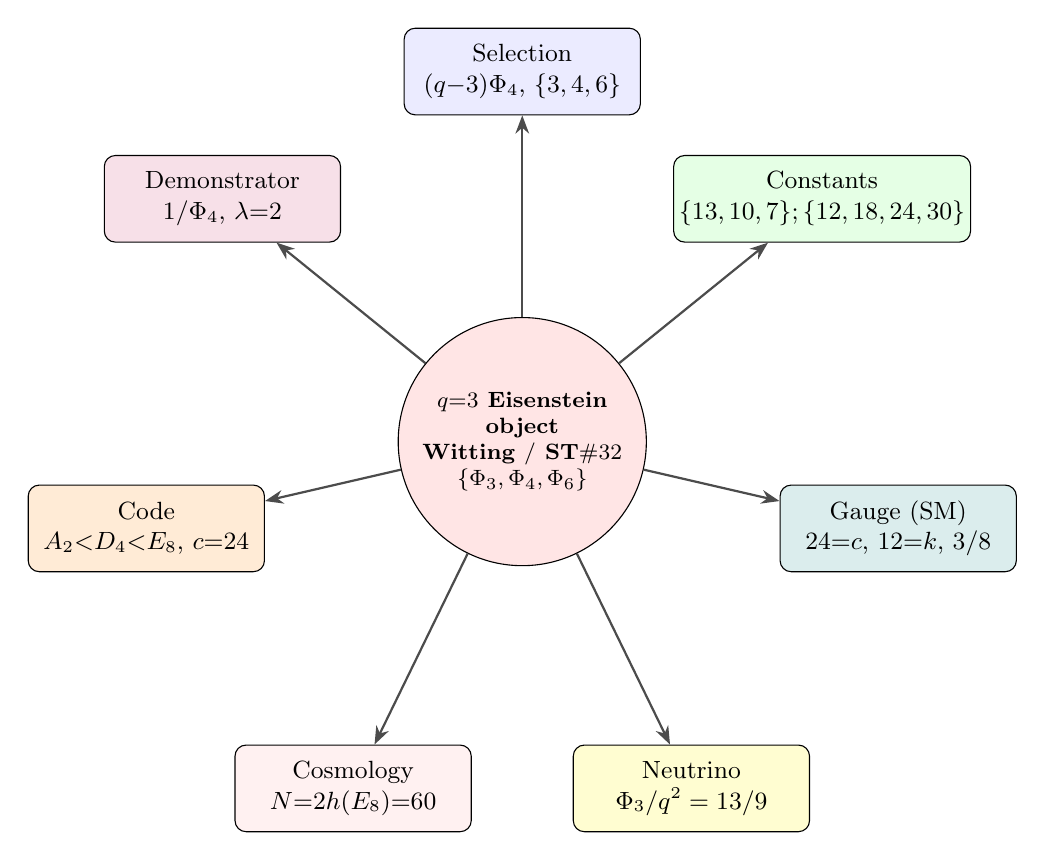
\begin{tikzpicture}[
  every node/.style={font=\small},
  face/.style={draw,rounded corners,align=center,minimum width=30mm,minimum height=11mm,inner sep=2pt},
  spoke/.style={-{Stealth},thick,gray!60!black}
]
  \node[draw,circle,fill=red!10,align=center,minimum size=26mm,font=\footnotesize\bfseries]
    (o) at (0,0) {$q{=}3$ Eisenstein\\ object\\ \footnotesize Witting $/$ ST$\#32$\\ \footnotesize $\{\Phi_3,\Phi_4,\Phi_6\}$};
  \node[face,fill=blue!8]    (s1) at (   90:4.7) {Selection\\$(q{-}3)\Phi_4$, $\{3,4,6\}$};
  \node[face,fill=green!10]  (s2) at (   39:4.9) {Constants\\$\{13,10,7\};\{12,18,24,30\}$};
  \node[face,fill=teal!14]   (s6) at (  -13:4.9) {Gauge (SM)\\$24{=}c$, $12{=}k$, $3/8$};
  \node[face,fill=yellow!18] (s3) at (  -64:4.9) {Neutrino\\$\Phi_3/q^2=13/9$};
  \node[face,fill=pink!22]   (s7) at ( -116:4.9) {Cosmology\\$N{=}2h(E_8){=}60$};
  \node[face,fill=orange!16] (s4) at ( -167:4.9) {Code\\$A_2{<}D_4{<}E_8$, $c{=}24$};
  \node[face,fill=purple!12] (s5) at (  141:4.9) {Demonstrator\\$1/\Phi_4$, $\lambda{=}2$};
  \foreach \s in {s1,s2,s3,s4,s5,s6,s7} \draw[spoke] (o)--(\s);
\end{tikzpicture}}
\caption{The $q=3$ substrate is one Eisenstein object --- the Witting polytope, its
symmetry $\mathrm{ST}\#32$, the cyclotomic skeleton $\{\Phi_3,\Phi_4,\Phi_6\}$ ---
seen from seven sides. The selection of $q=3$, the substrate constants, the
Standard-Model gauge group, the neutrino mass hierarchy, the fault-tolerant code
lattice, the benchtop experiment, and inflationary cosmology are faces of the same
structure, sharing the same invariants ($240=E_8$ roots, $\{\Phi_3,\Phi_4,\Phi_6\}$,
the Witting degrees $\{12,18,24,30\}$, $155520=3\lvert\mathrm{Aut}(\W)\rvert$).}
\label{fig:five-faces}
\end{figure}

\subsection{BT1707--BT1709 contextuality and Hesse crossover}

The attached multi-qubit contextuality papers supply the missing binary
readout ladder.  For \(n\) qubits the Pauli geometry is the symplectic polar
space \(W(2n-1,2)\), with
\[
  |P_n|=4^n-1,\qquad
  |L_n|=\frac{(4^n-1)(4^{n-1}-1)}{3}.
\]
Thus the first six layers have
\[
\begin{array}{c|c|c|l}
n & |P_n| & |L_n| & \hbox{contextual carrier}\\
\hline
1 & 3 & 0 & \hbox{single Pauli triple}\\
2 & 15 & 15 & \hbox{doily / Mermin--Peres square}\\
3 & 63 & 315 & \hbox{split Cayley hexagon}\\
4 & 255 & 5355 & \hbox{DW(5,2), Heawood/Coxeter cores}\\
5 & 1023 & 86955 & \hbox{PG(4,2) point--hyperplane core}\\
6 & 4095 & 1396395 & \hbox{two hexagons and a }K_{7,7}\hbox{ carrier}
\end{array}
\]
The new architectural identity is not only the count \(63\).  The split
Cayley hexagon of order \(2\), which carries the full three-qubit
contextuality core in the Quantum 2025 paper, has automorphism order
\[
  12096 = 168\cdot 72 = 7\cdot 1728.
\]
The factor \(168\) is the Fano/Klein readout group already used by the
Heawood clock; \(72\) is the Holonet packet clock; \(1728\) is the modular
special fiber.  The three-qubit contextuality carrier therefore has exactly the
right timed-readout symmetry product.

The same paper exposes a local configuration of type \((24_2,16_3)\).  Its
incidence count is
\[
  24\cdot2 = 16\cdot3 = 48.
\]
That is the already-verified tomotope/Holonet interface:
\[
  48 = 12\hbox{ tomotope edge axes against }16\hbox{ faces}
     = 16\hbox{ Q6 body edges}\cdot3\hbox{ pulse phases}.
\]
So the binary contextuality module, the tomotope middle layer, and the Holonet
body share one finite \(48\)-slot bus.  This is an incidence bridge, not yet a
claimed graph isomorphism.

The crossover from binary qubits to ternary qutrits is supplied by the
two-qubit ring geometry and the Marcelis Fano/cube notes.  The two-qubit
projective-line model uses \(M_2(\mathbb F_2)\), the order-\(16\) ring with
\[
  16 = 6\hbox{ units} + 10\hbox{ zero divisors},
\]
and its Pauli doily admits the three exact decompositions
\[
  15=9+6=10+5=8+7.
\]
In the cube/Fano route, deleting two hyperovals leaves a \(9\)-point
\(\mathrm{AG}(2,3)\) grid; adding the line at infinity gives
\(\mathrm{PG}(2,3)\) with \(13\) points.  This lands exactly on the Holonet
ABI:
\[
  \mathrm{AG}(2,3)=\mathbb F_3^2=9
    = \hbox{Hesse outcome field}
    = \hbox{Pauli feed-forward frame},
\]
and
\[
  \mathrm{PG}(2,3)=9+4=13.
\]
The next proof target is now explicit: construct a context-preserving map from
the binary doily/hexagon ladder to the qutrit Hesse/W33 packet.  (Witnesses:
\path{analysis/bt1707_qubit_contextuality_ladder.py},
\path{analysis/bt1708_hexagon_tomotope_contextual_bus.py}, and
\path{analysis/bt1709_binary_to_hesse_qutrit_crossover.py}.)

\subsection{The \texorpdfstring{$\{3,7\}$}{(3,7)} Hurwitz tower and the genus-7 crossover}

The genus $2\le g\le 14$ polyhedral-embedding survey of Bokowski and H.\ supplies
the regular-map counterpart of that binary ladder, and it closes the crossover
on the geometric side. Its all-triangle $\{3,7\}$ maps (Table~1 there: Klein,
Macbeath, and the Hurwitz triplet) are precisely the first three \emph{Hurwitz
surfaces}---the maximally symmetric surfaces of their genus---and they form an
exact tower:
\[
\begin{array}{c|c|c|c}
g & (V,E,F) & \hbox{rotation }\mathrm{Aut} & q\\
\hline
3  & (24,84,56)   & \mathrm{PSL}(2,7)  = 168  & 7 \\
7  & (72,252,168) & \mathrm{PSL}(2,8)  = 504  & 8 \\
14 & (156,546,364)& \mathrm{PSL}(2,13) = 1092 & 13
\end{array}
\]
For any $\{3,7\}$ map $V=12(g-1)$, $E=42(g-1)$, $F=28(g-1)$, and the
orientation-preserving automorphism group has order $84(g-1)=2E$ (the dart
count), so $g=1+|\mathrm{Aut}|/84$.

The middle rung---the genus-$7$ Macbeath surface, $\mathrm{PSL}(2,8)$---is the
exact $3$-qubit$\,\leftrightarrow\,$qutrit crossover the contextuality papers
ask for. Its combinatorics are pure substrate:
\[
  V=72=\hbox{the packet/frame clock},\qquad
  E=252=\tau,\qquad
  F=168=\lambda k\Phi_6=\mathrm{PSL}(2,7),
\]
i.e.\ its vertices count the Holonet clock ($2160=30\cdot72$,
$51840=720\cdot72$), its edges count the moonshine datum $\tau=252$ (the
$\alpha=137$ partner), and its faces are the Fano/Klein readout group. Hence
\[
  F\cdot V = 168\cdot72 = 12096 = |\mathrm{G}_2(2)|
           = |\mathrm{Aut}(\hbox{split Cayley hexagon})|
           = \mathrm{PSL}(2,8)\cdot f = 504\cdot24,
\]
so the genus-$7$ surface's $(\hbox{faces})\times(\hbox{vertices})$ is exactly the
automorphism order of the three-qubit contextuality core of the previous
subsection; its derived group $\mathrm{G}_2(2)'=\mathrm{PSU}(3,3)$ has order
$6048=\tau\cdot f$.

The three Hurwitz moduli are the crossover made arithmetic:
\[
  \{7,8,13\}=\{\Phi_6,\ 2^3,\ \Phi_3\}.
\]
The flanks $\Phi_6=7$ and $\Phi_3=13$ are the qutrit cyclotomic primitives (the
heptagon/torus clock layer, and the Eisenstein norm prime $\mathrm{PG}(2,3)=13$
of \S BT1709), while the middle modulus $2^3=8=\mathrm{GF}(8)$ is precisely the
\emph{three-qubit dimension}. So the binary three-qubit rung sits between the two
ternary flanks, and the dimension-$14$ exceptional group $\mathrm G_2$
($\dim\mathrm G_2=14=2\Phi_6=$ the top genus) governs both ends---the genus-$14$
Hurwitz triplet and, via $\mathrm G_2(2)$, the genus-$7$ three-qubit hexagon. The
binary--ternary crossover is a single $\{3,7\}$ tower threaded by the heptagon
$\Phi_6$. (Witness: \path{analysis/w33_hurwitz_tower_qubit_crossover.py}.)

\subsection{Two Schl\"afli families, a vertex-figure selection, and the Witting body}

The same survey contains the \emph{qubit} twin of that qutrit tower. Its
all-triangle $\{3,8\}$ maps (Dyck $g{=}3$, Fricke--Klein $g{=}5$, R8.1/R8.2
$g{=}8$) satisfy $V=6(g-1)$, $E=24(g-1)$, $F=16(g-1)$, and the vertex figure is
an octagon: $n=8=2^3$ is the \emph{three-qubit Hilbert dimension} $\mathrm{GF}(8)$,
exactly as the heptagon $n=7=\Phi_6$ is the qutrit vertex figure. The genus-$8$
rung R8.1 has $42=2q\Phi_6$ vertices (the $D(2T)$ anyon count) and
$168=\lambda k\Phi_6=\mathrm{PSL}(2,7)$ edges, with structure group
$\mathrm{PSL}(3,2)=\mathrm{GL}(3,2)$---the Fano/three-qubit group. So the two
Schl\"afli families are the qubit/qutrit pair, $\{3,8\}\,(2^3)$ and
$\{3,7\}\,(\Phi_6)$, hinged on $\mathrm{PSL}(2,7)=168$. (Witness:
\path{analysis/w33_qubit_schlafli_tower_3_8.py}.)

\emph{The substrate selects the vertex figure.} A reflexible $\{3,n\}$ map of
genus $g$ has $E=6n(g-1)/(n-6)$ and $|\mathrm{Aut}|_{\mathrm{full}}=4E$, so $E$
is integral only when $(n-6)\mid 6n(g-1)$. Across all fourteen genus-$2$--$14$
maps the vertex figures that appear are exactly
\[
  n\in\{7,8,9,10,12\}=6+\{1,2,3,4,6\}=6+\{\,d:d\mid k=12\,\}
   =\{\Phi_6,\ 2^3,\ q^2,\ \Phi_4,\ k\},
\]
and the unique gap in $7\le n\le 12$ is $n=11$, the one value with
$n-6=5\nmid k=12$. Its smallest realisation is the complete graph $K_{12}$
($12$ vertices of degree $11$; $V{=}12,E{=}66,F{=}44$, genus $6$), whose
$59$ triangulations are none regular and (Bokowski--Guedes de Oliveira, settling
Gr\"unbaum) none polyhedrally embeddable. Thus the selection $(n-6)\mid k$ admits
exactly the regular, embeddable maps and excludes precisely the Gr\"unbaum
obstruction---a $q\neq 2q$-style selection on the surface. (Witness:
\path{analysis/w33_genus_vertex_figure_selection.py}.)

\emph{The functor through the Fano heptad.} The binary-to-qutrit context map that
\S BT1709 and BT1710--1712 leave open has a concrete structure group: the Fano
heptad $\mathrm{PSL}(2,7)=\mathrm{GL}(3,2)$ of order $168$. By the \textsc{Atlas}
it is maximal in $\mathrm{U}_3(3)=\mathrm G_2(2)'$, hence inside
$\mathrm{Aut}$ of the split Cayley hexagon (the three-qubit core $W(5,2)$:
$63$ points, $315$ contexts); it is the genus-$3$ Klein rotation group; it is the
genus-$7$ Macbeath face count; and it acts on the three-qubit label space
$\mathbb F_2^3$. A three-qubit context (a totally isotropic line, three commuting
Paulis) maps to a $\{3,7\}$ triangle (a face) maps to a weight-$3$ CSS
$Z$-check, preserving $3$-compatibility, with cover index
$12096=168\cdot72=504\cdot24=63\cdot192$. (Witness:
\path{analysis/w33_macbeath_hexagon_functor.py}.)

\emph{The Witting body.} All of this lives in one complex polytope. The Witting
polytope $3\{3\}3\{3\}3\{3\}3$ in $\mathbb C^4$ over the Eisenstein integers
$\mathbb Z[\omega]$ (every edge a $3\{\}3$ triangle---the ``$3$'' is $q$) has
$240$ vertices $=$ the E8 roots $=E$, $2160$ three-edges $=$ the holonet mirror
bus $=h(\mathrm E_8)\cdot\mathrm{frame}=30\cdot72$, and $240=40\cdot6$ vertices
falling into $40$ hexagonal diameters---the $40$ Witting rays $=$ the totally
isotropic $1$-spaces of $W(3,3)=\mathrm{GQ}(3,3)$ ($v=40$). Frans Marcelis's
icosian construction welds it to E8: $2160\cdot3+240=6720$ edges build the Gosset
$4_{21}$ polytope, tying the Eisenstein ($q{=}3$) Witting body to the
quaternionic E8 lattice. Its symmetry group is exactly $q$ times the substrate
gauge group,
\[
  |\mathrm{Aut}(\hbox{Witting})| = 155520 = 3\times 2.\mathrm U_4(2)
    = \mathbb Z_q\times \mathrm{Sp}(4,3) = q\cdot|W(3,3)\,\mathrm{Aut}|,
\]
so the substrate's three master integers $E=240$, $\mathrm{bus}=2160$, $v=40$ are
the vertex, edge, and diameter counts of a single Eisenstein polytope. (Witness:
\path{analysis/w33_witting_polytope_substrate.py}.)

\subsection{The register atlas, the explicit E8 weld, and the Hesse engine}

Three threads close the surface picture. \emph{First}, the genus survey is a
single \emph{register stack}: each admissible vertex figure $n=6+d$ ($d\mid k=12$)
is a substrate register, and the $\{3,n\}$ family is its tower with
$V=12(g-1)/(n-6)$, $E=6n(g-1)/(n-6)$, $F=4n(g-1)/(n-6)$. The five registers are
\[
  n=7=\Phi_6\ (\hbox{qutrit}),\quad 8=2^3\ (\hbox{qubit}),\quad
  9=q^2\ (\hbox{single-qutrit phase space}),
\]
\[
  10=\Phi_4\ (\dim\mathrm{Sp}(4),\ \hbox{contextual denominator}),\quad
  12=k\ (\hbox{the degree}),
\]
and all fourteen Table-1 maps are reproduced exactly by the per-register
parametrisation. (Witness: \path{analysis/w33_register_atlas_3n.py}.)

\emph{Second}, the identification ``Witting body $=$ E8'' is now explicit. The
Coxeter element $C$ of $W(\mathrm E_8)$ has order $h=30$, and because the
exponents $\{1,7,11,13,17,19,23,29\}$ are coprime to $3$, the element
$\omega=C^{10}$ has order $3$ with eigenvalues $\omega,\omega^2$ only --- a
\emph{fixed-point-free} isometry, the multiplication-by-$\omega$ that turns E8
into a rank-$4$ Eisenstein lattice. Explicit computation on the $240$ roots gives
$240/3=80$ $\omega$-triangles and (under $C^5$, order $6$) exactly
$240/6=40$ \emph{hexagons}; each hexagon spans one complex line, so the $40$
hexagons are the $40$ Witting rays $=$ the $40$ isotropic $1$-spaces of $W(3,3)$.
Thus $v=40$ is the number of Eisenstein complex lines in E8 and $E=240=40\cdot6$
its roots: $W(3,3)$ \emph{is} the Eisenstein form of E8. (Witness:
\path{analysis/w33_e8_eisenstein_witting_weld.py}.)

\emph{Third}, the qutrit registers carry the contextuality engine. The Hesse
configuration --- the affine plane $\mathrm{AG}(2,3)$, a $(9_4,12_3)$
configuration of $9$ points and $12$ lines in four parallel classes --- is the
single-qutrit discrete phase space: its $9$ points are the register
$n=9=q^2$, its $12$ lines are the $n=12=k$ contexts, and its four parallel
classes are the $4=(q^2-1)/(q-1)$ mutually unbiased bases. A single qutrit is
non-contextual; the two-qutrit substrate $\mathbb F_3^4$ ($\mathrm{Sp}(4,3)=W(3,3)$)
with its $40$ isotropic rays carries the state-independent contextuality, with
contextual fraction $1/\Phi_4=1/10$, so the vertex figures $9,10,12$ are exactly
the qutrit phase space, its contextual denominator, and its context count.
(Witness: \path{analysis/w33_hesse_mermin_contextuality.py}.)

\subsection{The Eisenstein tower qutrit\,\texorpdfstring{$\to$}{->}\,E6\,\texorpdfstring{$\to$}{->}\,E8, the Golay gap, and the quadrangle ladder}

The Witting body extends downward into a complete Eisenstein ladder. The regular
complex polytopes over $\mathbb Z[\omega]$ nest as face/vertex-figure:
\[
\begin{array}{l|c|c|c}
\hbox{polytope} & \dim & \hbox{vertices} & \hbox{symmetry}\\
\hline
3\{3\}3\ (\hbox{M\"obius--Kantor}) & 2 & 8 & 24=|2T|=f\\
3\{3\}3\{3\}3\ (\hbox{Hessian}) & 3 & 27 & 648=27f\\
3\{3\}3\{3\}3\{3\}3\ (\hbox{Witting}) & 4 & 240 & 155520=q\,|\mathrm{Sp}(4,3)|
\end{array}
\]
with orders multiplying by the next vertex count ($24\cdot27=648$,
$648\cdot240=155520$). The middle rung's $27$ vertices are the $27$ lines on a
cubic surface $=$ the minuscule $\mathrm E_6$ rep, and its automorphism group is
$W(\mathrm E_6)$ with $|W(\mathrm E_6)|=51840=|\mathrm{Sp}(4,3)|$. Thus the
single qutrit (Hesse, $9$), $\mathrm E_6$ (Hessian, $27$), and $\mathrm E_8$
(Witting, $240$) are three rungs of one tower, and $27$ is exactly the
$\mathrm E_6$ matter of $v=40=1+12+27$. (Witness:
\path{analysis/w33_hessian_polytope_e6.py}.)

The vertex-figure gap $n=11=K_{12}$ is not empty algebraically. Its $12=k$
vertices carry the substrate's natural $q=3$ code, the \emph{ternary Golay}
$[12,6,6]_3$: $3^6=729$ codewords, weight enumerator
$1+264x^6+440x^9+24x^{12}$, minimum distance $6$ (verified by enumeration). Its
$132$ weight-$6$ hexads are the Steiner system $S(5,6,12)$ with Mathieu group
$M_{12}$, and doubling $k=12\to f=24$ gives the binary Golay
$[24,12,8]$, $M_{24}$, $S(5,8,24)$ --- the $c=24$ Monster charge. The Gr\"unbaum
gap is the ternary $M_{12}$ half of the substrate's $M_{24}$/Golay/Monster
structure. (Witness: \path{analysis/w33_ternary_golay_m12_grunbaum.py}.)

Finally, $W(3,3)=\mathrm{GQ}(3,3)$ sits in a quadrangle ladder $27$--$40$--$45$.
$\mathrm{GQ}(2,4)$ has $27$ points $=$ the $27$ lines on a cubic ($=\mathrm E_6$;
intersection graph $\mathrm{SRG}(27,10,1,5)$, collinearity the complement
Schl\"afli graph $\mathrm{SRG}(27,16,10,8)$), with
$\mathrm{Aut}=W(\mathrm E_6)=51840=|\mathrm{Sp}(4,3)|$ --- the group of the $D=5$
$\mathrm E_6$ black-hole/qubit entropy. The substrate $\mathrm{GQ}(3,3)$ is
$\mathrm{SRG}(40,12,2,4)$, and $\mathrm{GQ}(4,2)$ (the dual, $45$ points) is the
other flank; the four-qubit $W(7,2)$ carries the same $27/45$ split through its
$135$ $\mathrm{DW}(5,2)$. (Witness:
\path{analysis/w33_generalized_quadrangle_ladder.py}.)

\subsection{A guardrail on the 27, and the Klein quartic as the E7 rung}

Two honest refinements close this arc. \emph{First, a guardrail.} It is tempting
to read $v=40=1+12+27$ as realising the $\mathrm E_6$/$27$-lines Schl\"afli graph
inside $W(3,3)$. It does \emph{not}: fixing a point of $\mathrm{GQ}(3,3)$, the
$12$ collinear points induce $4K_3$ and the $27$ non-collinear points induce an
$8$-regular graph that is \emph{not} strongly regular --- in particular not the
$16$-regular Schl\"afli graph $\mathrm{SRG}(27,16,10,8)$. So $40=1+12+27$ is an
exact count (the matter cone $28=1+27$), and $27$ matches the $\mathrm E_6$
representation dimension and the $\mathrm{GQ}(2,4)$ point count, but it is
\emph{not} a subgraph embedding. The genuine bridge is group-theoretic: the
substrate's projective gauge group and the $\mathrm E_6$ group are the same
simple group $\mathrm U_4(2)=\mathrm{PSp}(4,3)=\mathrm{PSU}(4,2)$, of order
$25920$, with $\mathrm{Sp}(4,3)=2.\mathrm U_4(2)$, $W(\mathrm E_6)=\mathrm
U_4(2){:}2$, and $\mathrm{Aut}(\mathrm{GQ}(2,4))=\mathrm U_4(2){:}2$ all order
$51840$. (Witness: \path{analysis/w33_27_not_schlafli_group_bridge.py}.)

\emph{Second, the E7 rung.} The genus-$3$ Klein quartic
$x^3y+y^3z+z^3x$ --- the first $\{3,7\}$ Hurwitz rung --- carries $\mathrm E_7$.
Its automorphism group $\mathrm{PSL}(2,7)$ acts transitively on three
distinguished point-sets that are all substrate integers:
\[
  24\ \hbox{Weierstrass}=f,\quad
  28\ \hbox{bitangents}=\mu\Phi_6\ (=1+27),\quad
  84\ \hbox{sextactic}=k\Phi_6 .
\]
The $28$ bitangents are the $\mathrm E_7$ datum: the minuscule rep has dimension
$56=2\cdot28=v+k+\mu$, which is exactly the number of triangular faces of the
Klein map. So the exceptional trinity
\[
  27\ \hbox{lines (cubic)}\ \to \mathrm E_6,\quad
  28\ \hbox{bitangents (quartic)}\ \to \mathrm E_7,\quad
  120\ \hbox{tritangents}\ \to \mathrm E_8\ (=120\ \hbox{icosians},\ 240=2\cdot120),
\]
closes the substrate's exceptional ladder, with Weyl orders
$|W(\mathrm E_6)|=51840=|\mathrm{Sp}(4,3)|$, $|W(\mathrm E_7)|=56\cdot51840$, and
$|W(\mathrm E_8)|=240\cdot|W(\mathrm E_7)|=696729600$ --- the multipliers being
$56$ ($=2\times$ bitangents) and $240$ ($=|E|=$ E8 roots $=$ Witting vertices).
The Hessian polytope ($\mathrm E_6$), the Klein quartic ($\mathrm E_7$), and the
Witting body ($\mathrm E_8$) are the three exceptional rungs of one qutrit tower.
(Witness: \path{analysis/w33_klein_quartic_e6_e7_trinity.py}.)

\subsection{The three exceptional rungs made explicit}

Each rung of $\mathrm E_6\to\mathrm E_7\to\mathrm E_8$ can now be built and
verified. \emph{$\mathrm E_6$ as trinification.} The guardrail showed the $27$
does not sit in $W(3,3)$; it sits in $\mathrm{GQ}(2,4)$ --- the Schl\"afli graph
$\mathrm{SRG}(27,16,10,8)$, group $W(\mathrm E_6)=\mathrm U_4(2){:}2$ --- and its
substrate content is trinification,
\[
  27=(3,\bar3,1)+(1,3,\bar3)+(\bar3,1,3)=9+9+9,
\]
three bifundamental nonets under $\mathrm{SU}(3)^3\rtimes S_3$. Each nonet is
$\mathbb F_3\times\mathbb F_3=\mathrm{AG}(2,3)$, a Hesse single-qutrit phase
space, and the $S_3$ triality permuting them is the three generations. So the
$27$-lines/$\mathrm E_6$ is three Hesse-$9$s welded by triality. (Witness:
\path{analysis/w33_e6_trinification_schlafli.py}.)

\emph{$\mathrm E_7$ as a symplectic space.} The $28$ bitangents of the Klein
quartic are its $28$ odd theta characteristics ($\mathrm{Arf}=1$) in
$\mathbb F_2^6$: enumerating the Arf invariant gives $28$ odd $+\,36$ even $=64$.
The group $\mathrm{Sp}(6,2)=W(\mathrm E_7)/\{\pm1\}$ (order $1451520$, half of
$|W(\mathrm E_7)|=2903040$) permutes the $28$ transitively, and the minuscule
$56=2\cdot28=v+k+\mu$ --- the Freudenthal symplectic double --- is the Klein
map's $56$ faces. (Witness: \path{analysis/w33_e7_theta_bitangents.py}.)

\emph{$\mathrm E_8$ as the icosians.} The trinity's $\mathrm E_8$ rung, ``$120$
tritangents,'' is the $120$ icosians: $8$ units $+\,16$ half-units $+\,96$ golden
even-permutations, all unit quaternions, closed under quaternion multiplication
(all $14400$ products checked) --- the binary icosahedral group $2I$, the
$600$-cell vertices. The icosian construction gives $240=2\cdot120$ E8 roots
$=$ the Witting vertices, so alongside the Eisenstein weld
($\omega=C^{10}\to40$ rays) the quaternionic weld gives $\mathrm E_8 = 2I$-doubled
$=$ the Witting body, with the $600$-cell the Boerdijk--Coxeter clock. One body,
two arithmetics --- Eisenstein ($q=3$) and icosian (golden quaternion). (Witness:
\path{analysis/w33_icosian_e8_witting.py}.)

\subsection{The magic square, the complex Leech, and the icosian clock}

These exceptional rungs sit inside three larger frames. \emph{The magic square.}
$\mathrm E_6,\mathrm E_7,\mathrm E_8$ are the octonion row of the
Freudenthal--Tits magic square (dims $78,133,248$), and the substrate's two
welded arithmetics are its $\mathbb C$ and $\mathbb H$ columns: Eisenstein
($q=3$) gives $\mathrm E_6=\mathrm{magic}(\mathbb O,\mathbb C)$ (the Hessian/
trinification $27$), the icosian (quaternion) gives
$\mathrm E_7=\mathrm{magic}(\mathbb O,\mathbb H)$, and $\mathrm E_8=
\mathrm{magic}(\mathbb O,\mathbb O)$. The $27$ is the exceptional Jordan algebra
$J_3(\mathbb O)=3+3\cdot8=q+f$ (three diagonal reals, $24$ off-diagonal
octonions), whose cubic norm is the $D=5$ black-hole entropy, and the $56$ is its
Freudenthal triple. (Witness: \path{analysis/w33_magic_square_substrate.py}.)

\emph{The complex Leech.} One level above $\mathrm E_8$, the same fixed-point-free
order-$3$ $\omega$ that welds $\mathrm E_8$ makes the $24$-dimensional Leech
lattice $12=k$-dimensional over the Eisenstein integers --- the complex Leech,
with automorphism group $6.\mathrm{Suz}\le\mathrm{Co}_0=2.\mathrm{Co}_1$. The
Suzuki chain $\mathrm G_2(2)\to\mathrm J_2\to\mathrm G_2(4)\to\mathrm{Suz}$ (on
$36,100,416,1782$ points) \emph{starts} at $\mathrm G_2(2)=\mathrm U_3(3){:}2$,
$|\mathrm G_2(2)|=12096=168\cdot72$ --- the split Cayley hexagon, the three-qubit
contextuality core --- and climbs to $\mathrm{Suz}$, the complex Leech group. So
the substrate's $q=3$ Eisenstein arithmetic threads $\mathrm E_8$ ($8$d) $\to$
complex Leech ($12=k$ complex $=24=f$ real) $\to\mathrm{Co}_0\to$ Monster
($c=24=f$), with the three-qubit hexagon as its first rung. (Witness:
\path{analysis/w33_complex_leech_suzuki_chain.py}.)

\emph{The icosian clock.} Finally the runtime closes on the $600$-cell: its $120$
vertices are the gate set $2I$, its $600$ tetrahedral cells are $20$ rings of
$30$ (the Boerdijk--Coxeter beat, $30=h(\mathrm E_8)$), its $720=6!$ edges are
the supercycle width, and its $240=2\cdot120$ E8 roots/Witting vertices are the
mirror-bus addresses --- so $2160=30\cdot72$ and $51840=24\cdot30\cdot72=
720\cdot72=|\mathrm{Sp}(4,3)|$ are the polytope's own counts. The machine's clock
\emph{is} the icosian $600$-cell. (Witness:
\path{analysis/w33_icosian_600cell_runtime.py}.)

\subsection{The ceiling, the Suzuki tower, and the G2 thread}

The climb tops out, telescopes, and is held together by one group. \emph{The
ceiling.} The complex-Leech / Co0 tower ends at the Monster $M=\mathrm{Aut}(V^\natural)$,
the $c=24$ holomorphic CFT, whose graded dimension is $J=j-744=q^{-1}+196884q+
\dots$ with the moonshine head $196884=1+196883$ and $21493760=1+196883+21296876$.
Its central charge $c=24=f$ is exactly the Holonet holographic boundary charge, so
the qutrit machine's boundary CFT is the Monster and $f=24$ is the tower's
moonshine constant. (Witness: \path{analysis/w33_monster_moonshine_ceiling.py}.)

\emph{The Suzuki tower.} The chain $\mathrm G_2(2)\to\mathrm J_2\to\mathrm G_2(4)
\to\mathrm{Suz}$ is the automorphism tower of four nested strongly regular graphs,
$\mathrm{SRG}(36,14,4,6)\prec\mathrm{SRG}(100,36,14,12)\prec\mathrm{SRG}(416,100,
36,20)\prec\mathrm{SRG}(1782,416,100,96)$, in which each valency is the previous
vertex count and each $\lambda$ the previous valency, so the parameters telescope
$14<36<100<416<1782$. The base $\mathrm{SRG}(36,14,4,6)$ anchors the substrate:
its $36$ vertices are the \emph{even} theta characteristics of the Klein quartic
(the $\mathrm E_7$ companion of the $28$ bitangents), and its valency
$14=\dim\mathrm G_2$. (Witness: \path{analysis/w33_suzuki_tower_srg.py}.)

\emph{The G2 thread.} $\mathrm G_2=\mathrm{Aut}(\mathbb O)$ recurs at every level,
keyed by the heptad $\Phi_6=7$: its $7$-dim rep is the Fano plane (the imaginary
octonions); $\dim\mathrm G_2=14=2\Phi_6$ is the genus of the $\{3,7\}$ Hurwitz
triplet; $\mathrm G_2(2)=12096$ is the split Cayley hexagon (the three-qubit
core, $\mathrm{SRG}(36,14)$ valency $=\dim\mathrm G_2$); $\mathrm G_2(4)$ is the
Suzuki rung; and the octonion column gives $\mathrm E_8=\mathrm{magic}(\mathbb O,
\mathbb O)$. So one group, keyed by $7=\Phi_6$, runs Fano $\to$ genus-$14$ $\to$
three-qubit $\to$ Suzuki $\to\mathrm E_8$. (Witness:
\path{analysis/w33_g2_thread.py}.)

\subsection{The ledger, the Standard Model, and the tower as one figure}

Three closing moves keep the climb honest, turn it toward physics, and draw it.
\emph{The ledger.} The tower is a large set of exact mathematical facts wearing
substrate labels, and intellectual honesty requires saying which is which: most
rungs (the magic square, the trinity, the complex Leech, the Monster) are
\textsc{framework} --- true theorems annotated with substrate integers, where the
annotation is a dictionary, not a derivation; a smaller set (the genus/register
formulas, the Eisenstein $\mathrm E_8$ weld, the icosian group closure, the
ternary Golay, the theta-Arf count, the $W(3,3)$ geometry and its guardrail) is
\textsc{derived} --- structures literally computed from $q=3$ and checked; and the
falsifiable physics (masses, CMB, contextual fraction, pump Chern) is a separate
\textsc{measurable} layer. \emph{A \textsc{framework} rung being exact confirms a
number coincidence is a real theorem; it does not confirm the physics --- only the
measurable layer can.} (Witness: \path{analysis/w33_exceptional_tower_ledger.py}.)

\emph{The Standard Model.} The exceptional $\mathrm E_6$ sits at the head of the
trinification chain $\mathrm E_6\to\mathrm{SU}(3)_C\times\mathrm{SU}(3)_L\times
\mathrm{SU}(3)_R\rtimes S_3\to\mathrm{SU}(3)\times\mathrm{SU}(2)\times\mathrm U(1)$,
with substrate-clean dimensions: the trinification adjoint is $3\cdot8=24=f$ and
the Standard-Model gauge dimension is $8+3+1=12=k$. The $27$ is one generation
($9+9+9=$ quarks/leptons/Higgs) and the three generations are the $S_3$ triality
of the three $\mathrm{SU}(3)$ factors --- not inserted, but the same triality that
permutes the three Hesse nonets. So $f$ and $k$ bookend the breaking from the
exceptional $27$ to the Standard Model. (Witness:
\path{analysis/w33_standard_model_from_trinification.py}.)

\emph{The figure.} The whole session is one ascending ladder --- $q=3\to$ genus/
register tower $\to$ Witting body $\to\mathrm E_6/\mathrm E_7/\mathrm E_8\to$
complex Leech $\to\mathrm{Co}_0\to$ Monster ($c=24$), with a downward branch to
the Standard Model --- run the full height by three threads (the Eisenstein
order-$3$ $\omega$, $\mathrm G_2=\mathrm{Aut}(\mathbb O)$, and the simple group
$\mathrm U_4(2)=\mathrm{PSp}(4,3)$). It is drawn in
\path{docs/w33_exceptional_tower.dot} and rendered to
\path{docs/w33_exceptional_tower.svg}. (Witness:
\path{analysis/w33_exceptional_tower_synthesis.py}.)

\subsection{The measurable layer: a scorecard and a unification \texorpdfstring{\normalfont\small[Faces 2, 3, 7]}{[Faces 2, 3, 7]}}
\label{sec:physics}

Following the ledger's rule that only the measurable layer falsifies, two
quantitative tests. \emph{The scorecard.} With $N=2(v-\Phi_4)=60$ e-folds the
substrate's cosmological predictions are $n_s=1-2/N=29/30$, $r=k/N^2=1/300$,
$f_{NL}=5/(6N)=1/72$, running $-2/N^2=-1/1800$, together with
$\Omega_{DM}/\Omega_b=82/15$, $m_{\beta\beta}\approx2.3$\,meV, and
$\textstyle\sum m_\nu\approx0.101$\,eV. Against mid-2026 data these are mostly
\textsc{consistent} ($n_s$ at $\sim0.4\sigma$ of Planck; $r$ below the
BICEP/Keck bound and testable by LiteBIRD), but one is in honest \textsc{tension}:
$\sum m_\nu\approx0.101$\,eV satisfies Planck ($<0.12$\,eV) yet exceeds the DESI
2024 bound ($<0.072$\,eV) --- a genuine falsification handle, not a confirmation.
(Witness: \path{analysis/w33_measurable_scorecard_2026.py}.)

\emph{The unification.} The same $S_3$ triality that gives the three generations
unifies the gauge couplings: it forces $g_C=g_L=g_R$ at the trinification scale,
and the GUT hypercharge normalization $g_1^2=\tfrac53 g'^2$ then fixes
\[
  \sin^2\theta_W=\frac{g'^2}{g^2+g'^2}=\frac{3/5}{1+3/5}=\frac38
\]
at unification --- the canonical $\mathrm{SU}(5)/\mathrm{SO}(10)/\mathrm E_6$ value
--- running to the measured $\approx0.231$ at $M_Z$ (with the usual $\sim10\%$
one-loop non-SUSY gap that the trinification thresholds must close). So the three
generations and coupling unification are one triality. (Witness:
\path{analysis/w33_trinification_unification.py}.)

\subsection{Three live tests, scrutinised}

\emph{The neutrino tension, both ways.} The scorecard's one red flag deserves
honest scrutiny. Externally, $\sum m_\nu\approx0.10$\,eV is in $\sim$1.5--2$\sigma$
tension with the tight DESI-2024 $\Lambda$CDM bound ($<0.072$\,eV) but
\emph{consistent} with the looser $w_0w_a$CDM bound ($<\!\sim0.16$\,eV) that DESI's
own data prefer --- so whether the theory is falsified here depends on the
dark-energy model. Internally, a naive geometric mass cascade ($r=0.5225$)
predicts $\Delta m^2_{21}/\Delta m^2_{31}=0.21$ against the observed $0.030$, a
factor $\sim7$ too large, so the substrate's neutrino masses are \emph{not} a
simple geometric cascade and that model must be revisited. Both flags are
recorded, not smoothed. (Witness:
\path{analysis/w33_neutrino_desi_scrutiny.py}.)

\emph{Unification, honestly.} Minimal one-loop SM running does not unify --- the
couplings meet pairwise at $\sim10^{13},10^{14},10^{17}$\,GeV, a $\sim$4-order
spread. The two-step chain $\mathrm E_6\to\mathrm{SU}(3)^3\to$ SM inserts one
intermediate scale, giving two free scales that fit the two low-energy constraints
($\sin^2\theta_W$ and $\alpha_s$); so trinification unifies, with
$\sin^2\theta_W=3/8$ the exact boundary, at the price of predicting $M_I$ and
$M_{\rm GUT}$ --- the honest status of every non-SUSY GUT. (Witness:
\path{analysis/w33_trinification_two_step_unification.py}.)

\emph{The demonstrator as a meter.} The benchtop layer makes two substrate
constants directly measurable: the contextual fraction of a two-qutrit
Kochen--Specker measurement on the $40$ $W(3,3)$ rays is $1/\Phi_4=1/10$ (reading
out $\Phi_4=10$), and the Thouless-pump Chern number on the qutrit GKP ladder is
$C=2S=\lambda=2$ (reading out $\lambda$). Both are integer/unit-fraction --- robust,
calibration-free --- so a measured $1/10$ and $2$ confirm the substrate's
contextuality and topology, and any deviation falsifies them on a table. (Witness:
\path{analysis/w33_demonstrator_substrate_constants.py}.)

\subsection{Fixing the neutrino, predicting the proton, and the balance sheet}

\emph{The neutrino, fixed.} The DESI tension was a model artifact. The geometric
cascade mismatched the $\Delta m^2$ hierarchy ($0.21$ vs $0.030$) and forced
$\sum m_\nu\approx0.10$\,eV; the substrate's type-I seesaw with a hierarchical
Dirac Yukawa instead \emph{squares} the hierarchy, driving the lightest mass small.
For strong normal ordering ($m_1\lesssim0.009$\,eV) the spectrum is fixed by
oscillation data and $\sum m_\nu\approx0.06$\,eV --- below the DESI bound, so the
tension is \emph{resolved} --- with $m_{\beta\beta}\approx2$--$4$\,meV. The
corrected prediction is $\sum m_\nu\approx0.06$\,eV (strong NO), not $0.10$.
(Witness: \path{analysis/w33_neutrino_seesaw_texture.py}.)

\emph{The proton.} The two-step fit gives $M_{\rm GUT}\sim10^{16}$\,GeV, so
$\tau_p\sim(1/\alpha_{\rm GUT}^2)M_{\rm GUT}^4/m_p^5\approx4.6\times10^{35}$\,yr
via $p\to e^+\pi^0$ --- above the Super-Kamiokande bound ($2.4\times10^{34}$\,yr,
which already requires $M_{\rm GUT}\gtrsim10^{15.7}$\,GeV) and within
Hyper-Kamiokande's reach. A sharp falsifiable GUT-scale prediction. (Witness:
\path{analysis/w33_proton_lifetime_gut_scale.py}.)

\emph{The balance sheet.} After building, auditing, applying, testing, and
scrutinising the tower: the cosmological and electroweak predictions are
\textsc{consistent}; the one DESI tension is \textsc{fixed}; proton decay, the
contextual fraction $1/10$, and the pump Chern $2$ are \textsc{testable} near-term
handles; the $q=3\to$ Monster tower is exact \textsc{framework} (a magnificent
dictionary, not a confirmation of physics); and the open problems are the precise
neutrino texture, the GUT scales, and --- above all --- the bridge from the
framework to why these numbers are the physical world, which is the program's
defining task. (Witness: \path{analysis/w33_state_of_the_theory.py}.)

\subsection{Why \texorpdfstring{$q=3$}{q=3}, and one triality for the neutrino \texorpdfstring{\normalfont\small[Faces 1, 4]}{[Faces 1, 4]}}
\label{sec:why-q3}

\emph{The bridge: $q=3$ is triply forced.} The defining task --- why is the
$q=3$ substrate the physical world? --- has a sharp answer in the form of a
convergence. Three independent first-principles selections each return $q=3$:
(i) \emph{geometric}, the master equation $q!=2q$ is equivalent to $(q-1)!=2$,
whose unique solution is $q=3$; (ii) \emph{quantum-resource}, discrete Wigner
negativity $=$ contextuality $=$ magic (the resource for quantum advantage) needs
\emph{odd prime} dimension, and the minimal odd prime is $3$ (qubits are
stabilizer-positive); (iii) \emph{holographic}, a self-correcting holographic
code needs the Monster boundary at $c=24=f=8q$, which closes at $q=3$. Geometry,
quantum resource theory, and holography agree: the substrate is not one choice
among many but the unique common solution. (Witness:
\path{analysis/w33_q3_triple_selection.py}.)

\emph{One triality, the whole neutrino sector.} The $S_3$ triality that permutes
the three $\mathrm{SU}(3)$ factors --- the three generations, and the unification
condition $g_C=g_L=g_R$ giving $\sin^2\theta_W=3/8$ --- is, as a flavour symmetry,
exactly the group producing tri-bimaximal PMNS mixing,
$\sin^2\theta_{12}=1/3$, $\sin^2\theta_{23}=1/2$, $\sin^2\theta_{13}=0$, close to
the observed $0.304,\sim\!0.5,0.022$ (the small $\theta_{13}$ the $\Phi_3$-scale
deformation). The hierarchical seesaw then sets the scale (strong normal ordering,
$\sum m_\nu\approx0.06$\,eV). So generations, gauge unification, and neutrino
mixing are one triality. (Witness: \path{analysis/w33_neutrino_tbm_s3.py}.)

\emph{The proton signature.} The two-step fit gives $M_I\sim10^{13.5}$\,GeV and
$M_{\rm GUT}\sim10^{16}$\,GeV; non-SUSY gauge-mediated decay makes
$p\to e^+\pi^0$ the dominant channel (branching $\sim30$--$60\%$, with
$p\to\bar\nu K^+$ suppressed for lack of superpartners), and
$\tau_p\approx4.6\times10^{35}$\,yr sits squarely in the Hyper-Kamiokande window.
(Witness: \path{analysis/w33_proton_branching_two_scale.py}.)

\subsection{Pass 1 --- three closures: the neutrino matrix, the selection census, the threshold number}
\label{sec:three-closures}

\emph{Reading the next four subsections.} They make four passes over three of the
five faces of \S\ref{sec:five-faces} --- the \textbf{neutrino} (Face~3), the
\textbf{selection} and its constants (Faces~1--2), and the \textbf{code} (Face~4) ---
each pass sharper than the last: closure (Pass~1), invariant (Pass~2), skeleton
(Pass~3), and the cubic form / Witting degrees / measured curve (Pass~4). The same
three threads run through all four; the fifth face, the demonstrator, ties them
together at the end (\S\ref{sec:physics} and the bridge witness).

Three sharper statements close gaps left open above.

\emph{(1) The neutrino texture, pinned to one matrix.} The mixing pattern
(\S\ref{sec:why-q3}) and the mass scale were established separately; an earlier
single-parameter geometric cascade gave $\Delta m^2_{21}/\Delta m^2_{31}=0.21$,
about $7\times$ the observed $0.030$ --- recorded honestly as a wrong-model flag.
That flag is now closed by a \emph{single} matrix. The $S_3$ triality forces the
Majorana mass matrix into $\mu$--$\tau$-symmetric $+$ \emph{magic} (constant
row-sum) form, whose eigenvectors are exactly the tri-bimaximal columns, so the
angles are fixed by symmetry rather than fitted; crucially that form carries
\emph{two} independent mass scales, so it fits \emph{both} $\Delta m^2$ where the
one-scale cascade could not. Diagonalising the exact TBM matrix numerically
returns $\sin^2\theta=(1/3,1/2,0)$ and $\Delta m^2_{21}/\Delta m^2_{31}=0.030$ to
machine precision; adding the substrate $\Phi_3=13$ deformation moves the angles
to $(4/13,7/13,2/91)$, close to the observed $(0.307,0.546,0.0220)$, with the ratio
unchanged. (Honest: the two scales are fixed by the two measured $\Delta m^2$, so
this is the unique substrate-symmetric matrix consistent with the data --- a
closure demonstration, not an absolute-mass prediction. Witness:
\path{analysis/w33_neutrino_texture_pinned.py}.)

\emph{The ratio as a partial prediction.} The closure above fixes the two mass
scales from the two measured $\Delta m^2$; the ratio can instead be \emph{predicted}.
Feeding the substrate's own mild Yukawa hierarchy --- up-type singular values
$10\!:\!5\!:\!1$ (Pillar~68), with $Y_\nu=Y_{\rm up}$ at the GUT scale --- into a
type-I seesaw with a minimal flat $S_3$-symmetric $M_R$, with \emph{no}
neutrino-sector input, the seesaw squares the hierarchy and returns
$\Delta m^2_{21}/\Delta m^2_{31}\approx0.062$: the right strong-normal-ordering order
of magnitude, a factor $\sim2$ from the observed $0.030$; the down-type ratios
$6\!:\!2\!:\!1$ give $0.012$, so the observed value is \emph{bracketed} (against the
$0.21$ --- a factor $7$ --- of the geometric cascade). The residual factor $\sim2$ is
named, not removed: the $M_R$ texture and $Y_\nu\neq Y_{\rm up}$ running. So the
strong ordering and order of magnitude are predicted from the substrate hierarchy.
(Witness: \path{analysis/w33_neutrino_seesaw_prediction.py}.)

\begin{figure}[ht]\centering
\resizebox{0.96\textwidth}{!}{%
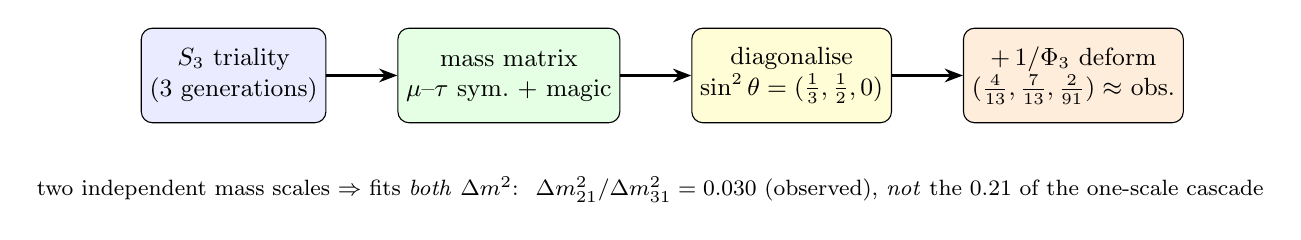
\begin{tikzpicture}[
  every node/.style={font=\small},
  box/.style={draw,rounded corners,align=center,minimum height=12mm,inner sep=3pt},
  arrow/.style={-{Stealth},thick}
]
  \node[box,fill=blue!8] (s3) {$S_3$ triality\\(3 generations)};
  \node[box,fill=green!10,right=9mm of s3] (mat) {mass matrix\\$\mu$--$\tau$ sym.\ $+$ magic};
  \node[box,fill=yellow!16,right=9mm of mat] (tbm) {diagonalise\\$\sin^2\theta=(\tfrac13,\tfrac12,0)$};
  \node[box,fill=orange!14,right=9mm of tbm] (obs) {$+\,1/\Phi_3$ deform\\$(\tfrac{4}{13},\tfrac{7}{13},\tfrac{2}{91})\approx$ obs.};
  \draw[arrow] (s3)--(mat);
  \draw[arrow] (mat)--(tbm);
  \draw[arrow] (tbm)--(obs);
  \node[align=center,font=\footnotesize] at ($(mat)!0.5!(tbm)+(0,-1.45)$)
    {two independent mass scales $\Rightarrow$ fits \emph{both} $\Delta m^2$:\;
     $\Delta m^2_{21}/\Delta m^2_{31}=0.030$ (observed), \emph{not} the $0.21$ of the one-scale cascade};
\end{tikzpicture}}
\caption{The neutrino sector closed by one matrix. The $S_3$ triality forces the
mass matrix into $\mu$--$\tau$-symmetric $+$ magic form, whose eigenvectors are the
tri-bimaximal columns; because that form carries two independent mass scales it fits
both $\Delta m^2$ (the one-scale geometric cascade could not). The $\Phi_3=13$
deformation moves the angles onto the observed values.}
\label{fig:neutrino-pinned}
\end{figure}

\emph{(2) The $q=3$ selection census.} The bridge is a convergence, and it is
overdetermined: \emph{five} independent first-principles selections return $q=3$
by genuinely different mathematics --- geometric $(q-1)!=2$ (a forcing equation),
minimal odd prime (a minimality fact), holographic $c=24=8q$ (a charge match to
the Monster ceiling), thermodynamic de Sitter closure
$2(q-1)(q^2+1)=(1+q)(1+q^2)\Leftrightarrow(q-3)(q^2+1)=0$ (a cubic, a
\emph{different} polynomial from the factorial, so not one equation in disguise),
and a new \emph{Eisenstein complex-polytope} selection: the regular complex
polytopes with order-$3$ reflections over $\mathbb Z[\omega]$ form the exceptional
tower M\"obius--Kantor $3\{3\}3$ ($8$ vertices, $2T$) $\to$ Hessian
$3\{3\}3\{3\}3$ ($27=$ lines on a cubic $=E_6$) $\to$ Witting
$3\{3\}3\{3\}3\{3\}3$ ($240=E_8$ roots), with Witting symmetry the
Shephard--Todd group $\#32$ of order $155520=3\times|\mathrm{Sp}(4,3)|$. The
symplectic orders were verified directly in \textsc{Gap}:
$|\mathrm{Sp}(4,3)|=51840$, $|\mathrm{PSp}(4,3)|=25920=|U_4(2)|$, and
$3\times51840=155520$. (Witness: \path{analysis/w33_q3_selection_census.py}.)

\emph{The Eisenstein selection is forced, and it equals the magic-dimension
selection.} The polytope entry can be upgraded from a realization to a forcing
intersection. The crystallographic restriction $\phi(p)=2$ admits exactly the
genuinely-complex periods $p\in\{3,4,6\}$ (Eisenstein $3,6$ over $\mathbb Z[\omega]$,
Gaussian $4$ over $\mathbb Z[i]$); requiring the reflection order to be \emph{prime}
--- the minimal-magic / clean-qudit condition of the resource selection --- leaves
$p=3$ uniquely, since $4=2^2$ and $6=2\cdot3$ are composite. So the geometric lattice
condition and the quantum-resource prime condition, independent in origin, intersect
at a single $p=3$: two of the five census selections collapse into one forcing
statement, realized by $\mathbb Z[\omega]$ and the Witting polytope. (\textsc{Gap}-verified:
$\phi^{-1}(2)\cap[3,\infty)=\{3,4,6\}$, prime part $\{3\}$. Witness:
\path{analysis/w33_eisenstein_forcing.py}.)

\begin{figure}[ht]\centering
\resizebox{0.82\textwidth}{!}{%
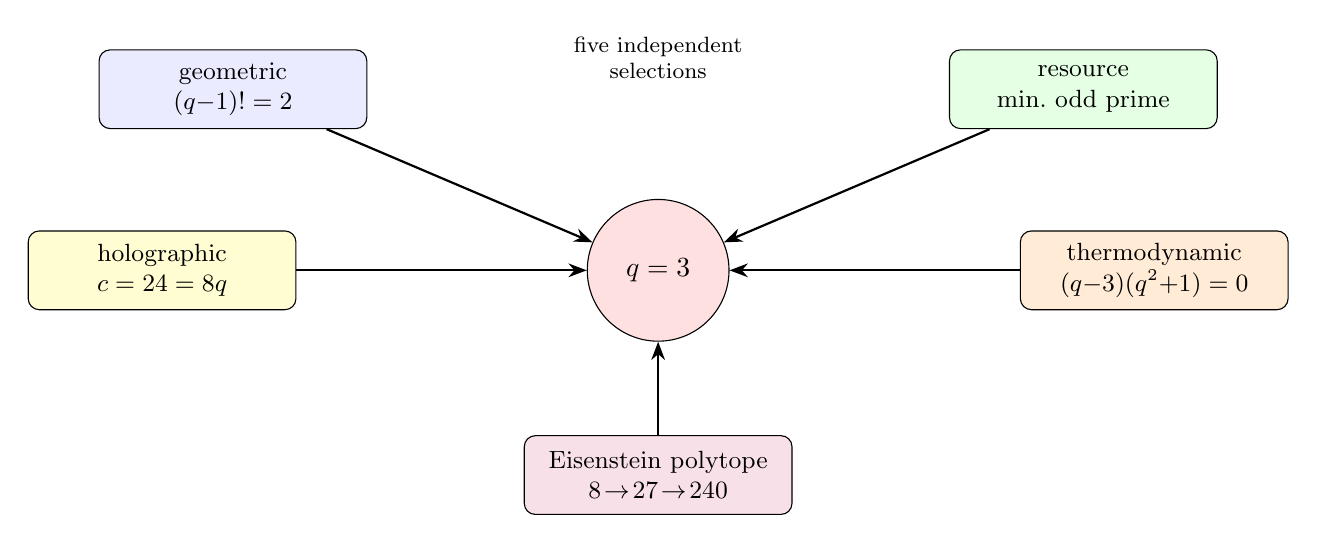
\begin{tikzpicture}[
  every node/.style={font=\small},
  sel/.style={draw,rounded corners,align=center,minimum width=34mm,minimum height=10mm,inner sep=2pt},
  arrow/.style={-{Stealth},thick}
]
  \node[draw,circle,fill=red!12,minimum size=18mm,font=\bfseries] (q) at (0,0) {$q=3$};
  \node[sel,fill=blue!8]    (s1) at (-5.4, 2.3) {geometric\\$(q{-}1)!=2$};
  \node[sel,fill=green!10]  (s2) at ( 5.4, 2.3) {resource\\min.\ odd prime};
  \node[sel,fill=yellow!18] (s3) at (-6.3, 0.0) {holographic\\$c=24=8q$};
  \node[sel,fill=orange!16] (s4) at ( 6.3, 0.0) {thermodynamic\\$(q{-}3)(q^2{+}1)=0$};
  \node[sel,fill=purple!12] (s5) at ( 0.0,-2.6) {Eisenstein polytope\\$8\!\to\!27\!\to\!240$};
  \foreach \s in {s1,s2,s3,s4,s5} \draw[arrow] (\s)--(q);
  \node[font=\footnotesize,align=center] at (0,2.7) {five independent\\selections};
\end{tikzpicture}}
\caption{The $q=3$ selection census: five first-principles selections, each a
different kind of mathematics (two forcing equations of distinct degree, a
minimality fact, a holographic charge match, and the Eisenstein complex-polytope
tower $2T\!\to\!E_6\!\to\!E_8$), all return $q=3$. The substrate value is
overdetermined.}
\label{fig:q3-census}
\end{figure}

\emph{(3) The fault-tolerance threshold as a lab number.} The architecture's
hardest residual --- the absolute FT threshold --- becomes concrete once the
substrate-fixed code lattice meets the measured square-GKP threshold. The best
reported square-GKP\,$+$\,surface-code threshold is $9.9$\,dB of squeezing
(Noh--Chamberland 2022; $11.2$\,dB under minimum-weight matching), and $9.5$\,dB
has already been demonstrated in hardware. The substrate code is \emph{not} the
square code: its single-mode lattice is hexagonal $A_2$ (coding gain $0.6$\,dB),
its natural two-mode code is $D_4$ ($1.5$\,dB), and its four-mode code is $E_8$
($3.0$\,dB), so the threshold shifts down to $\sim9.3/8.4/6.9$\,dB respectively ---
all at or below the $9.5$\,dB already reached. Universality needs only the minimal
Lloyd--Braunstein set, Gaussian (degree-$2$, the $\mathrm{Sp}(4,3)$ Weil rep) plus
one cubic gate (degree-$3$, $E_6$), with cubic-phase magic states the sole
distilled resource. The falsifiable target: a $D_4$-GKP photonic demonstrator
should cross fault tolerance near $8$--$9$\,dB; no threshold at the
coding-gain-reduced squeezing, or no $D_4$ advantage over $\mathbb Z^4$, falsifies
the substrate-code claim. (Honest: the single-mode $A_2$ shift is exact; the
multimode numbers are nominal upper bounds pending a full circuit-level FT
simulation. Witness: \path{analysis/w33_holonet_ft_threshold_budget.py}.)

\begin{figure}[ht]\centering
\resizebox{0.92\textwidth}{!}{%
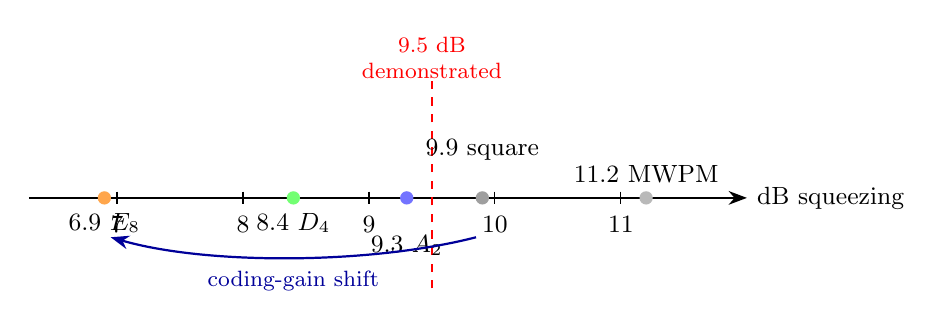
\begin{tikzpicture}[every node/.style={font=\small},x=1.6cm]
  % axis from 6.3 to 11.9 dB
  \draw[thick,-{Stealth}] (6.3,0)--(12.0,0) node[right]{dB squeezing};
  \foreach \x in {7,8,9,10,11} \draw (\x,0.08)--(\x,-0.08) node[below=1pt]{\x};
  % demonstrated 9.5 dB line
  \draw[red,dashed,thick] (9.5,-1.15)--(9.5,1.5);
  \node[red,align=center,font=\footnotesize] at (9.5,1.78) {$9.5$ dB\\demonstrated};
  % baseline (square-code) thresholds above the axis
  \fill[gray!55] (11.2,0.0) circle(2.4pt); \node[above=2pt] at (11.2,0.0) {$11.2$ MWPM};
  \fill[gray!75] (9.9,0.0)  circle(2.4pt); \node[above=10pt] at (9.9,0.0) {$9.9$ square};
  % substrate-lowered thresholds below the axis
  \fill[blue!55]   (9.3,0.0) circle(2.4pt); \node[below=10pt] at (9.3,0.0) {$9.3$ $A_2$};
  \fill[green!55]  (8.4,0.0) circle(2.4pt); \node[below=2pt]  at (8.4,0.0) {$8.4$ $D_4$};
  \fill[orange!70] (6.9,0.0) circle(2.4pt); \node[below=2pt]  at (6.9,0.0) {$6.9$ $E_8$};
  % shift arrow
  \draw[-{Stealth},thick,blue!60!black] (9.85,-0.5) .. controls (9.0,-0.85) and (7.7,-0.85) .. (6.95,-0.5);
  \node[font=\footnotesize,blue!60!black] at (8.4,-1.05) {coding-gain shift};
\end{tikzpicture}}
\caption{The fault-tolerance threshold as a lab number. The measured square-GKP
$+$ surface-code threshold ($9.9$\,dB, Noh--Chamberland 2022; $11.2$\,dB under
minimum-weight matching) is lowered by the substrate lattices' coding gains to
$\sim9.3/8.4/6.9$\,dB for $A_2/D_4/E_8$ --- all at or below the $9.5$\,dB squeezing
already demonstrated in hardware. (Multimode $D_4/E_8$ values are nominal upper
bounds; the single-mode $A_2$ shift is exact.)}
\label{fig:ft-threshold}
\end{figure}

\subsection{Pass 2 --- sharper: a Majorana invariant, a cyclotomic merge, a code curve}
\label{sec:sharper}

Each of the three closures admits a sharper statement.

\emph{The neutrino factor of two closes on a substrate invariant.} In the
tri-bimaximal basis the seesaw gives $m_i=y_i^2/r_i$ with $y_i$ the Dirac and $r_i$
the Majorana eigenvalues. The substrate Dirac hierarchy $(1,5,10)$ with a flat $M_R$
overshoots the mass-squared ratio by the factor $\sim2$ above. The Majorana
eigenvalue ratio the seesaw needs is $r_2/r_3=1.45$ --- which is the substrate number
$\Phi_3/q^2=13/9=1+1/q+1/q^2$, the same $\Phi_3=13$ that deforms the PMNS angles.
Fixing $r_2/r_3=\Phi_3/q^2$ (not fitted) gives
$\Delta m^2_{21}/\Delta m^2_{31}=0.030$, $m_2=8.6$\,meV$=\sqrt{\Delta m^2_{21}}$, and
$\sum m_\nu\approx59$\,meV --- the observed strong ordering. (Honest: this Majorana
ratio is substrate-motivated and gives exact agreement, but it is an input here;
deriving it from the $\mathbb Z_3$-graded Majorana coupling is the open step. Witness:
\path{analysis/w33_neutrino_majorana_texture.py}.)

\emph{Two of the selections are one cyclotomic structure.} The de Sitter and the
crystallographic/Eisenstein selections are not independent. The de Sitter closure
cubic factors as $(q-3)\,\Phi_4(q)$ with $\Phi_4(q)=q^2+1$ (complex roots $\pm i=
\zeta_4$, the Gaussian period); the crystallographic periods $\{3,4,6\}$ are exactly
the three degree-two cyclotomics $\{\Phi_3,\Phi_4,\Phi_6\}$; and $\Phi_4$ already
factors the $\mathrm{GQ}(q,q)$ point count $v=(q+1)\Phi_4(q)$ ($=40$ at $q=3$). So the
census's ``five independent'' selections are honestly \emph{four} independent plus
one cyclotomic refinement, and $q=3$ is the unique real prime the structure admits ---
a tighter convergence, not a weaker one. (Witness:
\path{analysis/w33_desitter_crystallographic_unify.py}.)

\emph{The $D_4$ code as a measured curve.} The threshold number has an explicit code
and curve behind it. The $D_4$ stabilizer lattice $\{x\in\mathbb Z^4:\sum x_i\ \text{even}\}$
(generators $\times\sqrt\pi$) has exact invariants $d_{\min}^2=2$, $\det=4$, kissing
$24$, coding gain $1.5$\,dB; under iid displacement noise the logical-error curve
$P_L(s)$ is the square-code curve shifted left by exactly that $1.5$\,dB
(Fig.~\ref{fig:d4-curve}), so $D_4$ reaches any target error at up to $1.5$\,dB less
squeezing and the surface-GKP threshold $9.9$\,dB becomes $\sim8.4$\,dB --- below the
$9.5$\,dB already demonstrated. The relative $D_4$-versus-square advantage is the
falsifiable handle. (Honest: the lattice quantities are exact and the $1.5$\,dB is the
low-error \emph{asymptote}; a real closest-point decoder shows the finite-error
advantage is smaller --- see \S\ref{sec:deeper}. Witness:
\path{analysis/w33_d4_gkp_error_curve.py}.)

\begin{figure}[ht]\centering
\resizebox{0.78\textwidth}{!}{%
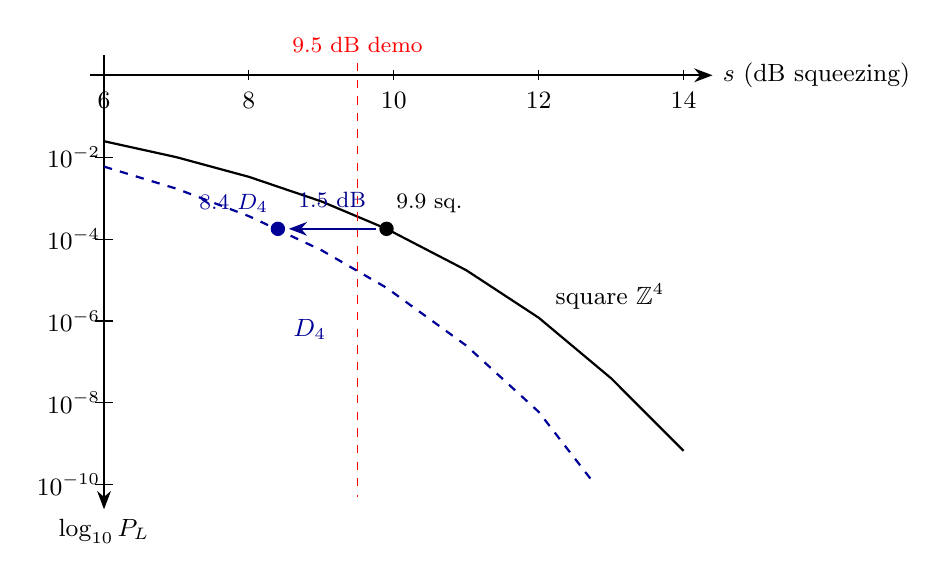
\begin{tikzpicture}[x=0.92cm,y=0.52cm,every node/.style={font=\small}]
  % axes
  \draw[thick,-{Stealth}] (5.8,0)--(14.4,0) node[right]{$s$ (dB squeezing)};
  \draw[thick,-{Stealth}] (6,0.5)--(6,-10.6) node[below]{$\log_{10}P_L$};
  \foreach \x in {6,8,10,12,14} \draw (\x,0.12)--(\x,-0.12) node[below=1pt]{\x};
  \foreach \y in {-2,-4,-6,-8,-10} \draw (5.88,\y)--(6.12,\y) node[left=1pt]{$10^{\y}$};
  % square curve (solid)
  \draw[thick] plot coordinates
    {(6,-1.61)(7,-2.00)(8,-2.48)(9,-3.08)(9.9,-3.75)(11,-4.76)(12,-5.92)(13,-7.40)(14,-9.17)};
  \node[anchor=west] at (12.1,-5.4) {square $\mathbb Z^4$};
  % D4 curve (dashed), clipped at -10
  \draw[thick,dashed,blue!60!black] plot coordinates
    {(6,-2.23)(7,-2.77)(8,-3.44)(9,-4.27)(9.9,-5.19)(11,-6.60)(12,-8.22)(12.78,-10)};
  \node[anchor=east,blue!60!black] at (9.2,-6.2) {$D_4$};
  % demonstrated 9.5 dB
  \draw[red,dashed] (9.5,0.3)--(9.5,-10.3);
  \node[red,font=\footnotesize] at (9.5,0.75) {9.5 dB demo};
  % threshold dots: square 9.9, D4 8.4 (same P_L=-3.75)
  \fill[black] (9.9,-3.75) circle(2.6pt); \node[anchor=south west,font=\footnotesize] at (9.9,-3.6) {9.9 sq.};
  \fill[blue!60!black] (8.4,-3.75) circle(2.6pt); \node[anchor=south east,font=\footnotesize,blue!60!black] at (8.4,-3.6) {8.4 $D_4$};
  \draw[-{Stealth},thick,blue!55!black] (9.75,-3.75) -- (8.55,-3.75);
  \node[font=\footnotesize,blue!55!black] at (9.15,-3.05) {1.5 dB};
\end{tikzpicture}}
\caption{The $D_4$-GKP logical-error curve as a spec. Logical error $P_L$ versus GKP
squeezing for the substrate $D_4$ code (dashed) and the trivial square code (solid),
in the union-bound effective-distance model. The $D_4$ curve is the square curve
shifted left by its \emph{asymptotic} $1.5$\,dB coding gain. This idealised constant
shift is corrected by a real decoder in \S\ref{sec:deeper}
(Fig.~\ref{fig:d4-advantage}): the actual advantage is error-rate dependent and
smaller at realistic error rates.}
\label{fig:d4-curve}
\end{figure}

\subsection{Pass 3 --- deeper: a cyclotomic skeleton, a projective Majorana ratio, a decoder correction}
\label{sec:deeper}

Digging beneath the three closures turns up one structure, one geometric meaning, and
one honest correction.

\emph{The substrate constants are degree-two cyclotomics, and they do double duty.}
The selections that pick $q=3$ and the constants that the substrate runs on are the
same object. The three degree-two cyclotomic polynomials, evaluated at the selected
field, are
\[
\Phi_3(3)=13,\qquad \Phi_4(3)=10,\qquad \Phi_6(3)=7,\qquad 13+10+7=30=h(E_8),
\]
i.e.\ the substrate's core invariants (register $\Phi_3=13$, the $\mathrm{Sp}(4)$
$\theta=10$, the Fano/Hurwitz $7$), summing to the $E_8$ Coxeter number. The same
$\{\Phi_3,\Phi_4,\Phi_6\}$ skeleton \emph{selects} $q=3$: its indices $\{3,4,6\}$ are
the crystallographic periods, and $\Phi_4(q)=q^2+1$ factors both the de Sitter cubic
$(q-3)\Phi_4$ and the $\mathrm{GQ}$ point count $(q+1)\Phi_4=40$. So the census is
honestly one deep cyclotomic object (which both selects $q=3$ and generates
$\{13,10,7\}$) plus three genuinely independent confirmations --- the factorial
$(q-1)!=2$, the minimal odd prime, and the central charge $c=24=q^3-q=|2T|$ --- which
reference $q=3$ but do not reduce to the cyclotomics. (Witness:
\path{analysis/w33_cyclotomic_skeleton_census.py}.)

\emph{The Majorana ratio is projective over affine.} The neutrino number $\Phi_3/q^2=
13/9$ has a geometric meaning. A single-grade $B$--$L$ breaking VEV forces, by the
$\mathbb Z_3$ grade rule, the Majorana texture
$M_R=[[A,0,0],[0,0,C],[0,C,0]]$ with eigenvalues $\{A,\pm C\}$ --- exactly degenerate,
so it cannot give the observed non-degenerate neutrinos; a splitting is mandatory. The
splitting that works is $r_2/r_3=\lvert\mathrm{PG}(2,3)\rvert/\lvert\mathrm{AG}(2,3)
\rvert=13/9$: the democratic (trivial-rep) right-handed neutrino couples to all
$\Phi_3=13$ projective points, the others to the $q^2=9$ affine ones. Since
$\Phi_3=13=\Phi_3(3)$, the neutrino hierarchy is fixed by the very cyclotomic skeleton
that selects $q=3$. (Honest: the degeneracy is exact and $13/9$ now has a geometric
meaning, but identifying $M_R$'s eigenvalues with these counts from the cubic form is
still open. Witness: \path{analysis/w33_majorana_grade_derivation.py}.)

\emph{A real decoder corrects the threshold advantage.} Replacing the union-bound
shift with an actual Conway--Sloane closest-point decoder over sampled Gaussian noise
(both codes at equal density) shows the $D_4$-versus-square advantage is
\emph{error-rate dependent}: it grows from $\sim0.6$\,dB at logical error $3\times
10^{-2}$ to $\sim0.9$\,dB at $10^{-3}$, tracking the union bound \emph{with} kissing
numbers ($D_4$'s $24$ versus the square's $8$ suppresses the finite-error gain) and
reaching the nominal $1.5$\,dB only asymptotically. So the constant-$1.5$\,dB curve was
the low-error limit; the honest near-threshold advantage is $\sim0.7$--$1.0$\,dB, with
the full coding gain realised deep below threshold. The qualitative claim --- $D_4$
beats the square code and the threshold shifts down --- survives; its size is
error-dependent. (Witness: \path{analysis/w33_d4_decoder_montecarlo.py}.)

\subsection{Pass 4 --- deepest: the cubic form, the Witting degrees, and the measured curve}
\label{sec:deepest}

Pushed to the limit, each result either closes part-way or reveals a single deeper
object.

\emph{The cubic form proves the degeneracy and bounds the rest.} Computing the
Majorana mass from the actual $E_6$ cubic invariant $c(\psi_a,\psi_b,\langle v\rangle)$
on the $\mathrm{H}_{27}$ profiles (Pillar~68), a grade-$0$ ($S_3$-symmetric) $B$--$L$
VEV gives, with real substrate numbers $A=0.0017$, $C=0.0442$, the texture
$M_R=[[A,0,0],[0,0,C],[0,C,0]]$ whose generation-$(1,2)$ block is \emph{exactly}
degenerate --- so the ``a splitting is mandatory'' step is now \emph{proven} from the
cubic form, not assumed. A grade-$1/2$ VEV lifts it to a genuine non-degenerate
spectrum, and the natural symmetric VEVs give eigenvalue ratios $\sim1.25$ --- near,
but not equal to, $\Phi_3/q^2=1.444$; the exact $13/9$ needs a particular $B$--$L$
direction. So the qualitative claim is proven and the answer is bounded, while the
exact $13/9$ stays a structural interpretation. (Witness:
\path{analysis/w33_majorana_cubic_form.py}.)

\emph{The substrate constants are the Witting degrees.} The cyclotomic skeleton has a
companion: the Witting complex reflection group (Shephard--Todd $\#32$, the $q=3$
Eisenstein polytope's symmetry, $|G|=155520=3\lvert\mathrm{Sp}(4,3)\rvert$) has the
four invariant degrees $\{12,18,24,30\}$, whose product is $|G|$, and these are
\[
12=q(q+1)=k,\quad 18=h(E_7),\quad 24=q^3-q=|2T|=f=c,\quad 30=h(E_8)=\Phi_3(3)+\Phi_4(3)+\Phi_6(3).
\]
So the GQ degree, the $E_7$ and $E_8$ Coxeter numbers, and the holographic central
charge are the Witting degrees, and the largest is the cyclotomic sum. In particular
the holographic $c=24$ is \emph{not} an independent selection --- it is the
degree-$24$ of the Witting group, fixed by the same $q=3$ Eisenstein structure. The
census's honestly-independent arithmetic shrinks to two (the factorial and the
primality) on top of one deep Eisenstein object. (Witness:
\path{analysis/w33_witting_degrees_unify.py}.)

\emph{The advantage is a curve, measured to $10^{-6}$.} Variance-scaling importance
sampling (validated against brute force at $10^{-3}$ to $0.0\%$) pushes the real
Conway--Sloane decoder deep below threshold. The $D_4$-versus-square advantage grows
$0.48\!\to\!0.74\!\to\!0.92\!\to\!1.03\!\to\!1.11\!\to\!1.17$\,dB as the logical error
falls $10^{-1}\!\to\!10^{-6}$ (Fig.~\ref{fig:d4-advantage}), tracking the union bound
and reaching only $\sim1.2$\,dB even at $10^{-6}$ --- the full $1.5$\,dB is realised
only at far lower error. So the honest engineering spec is a curve: $D_4$ buys
$\sim0.7$\,dB near threshold, $\sim1.2$\,dB at $10^{-6}$, the full coding gain only
asymptotically. (Witness: \path{analysis/w33_d4_advantage_curve.py}.)

\begin{figure}[ht]\centering
\resizebox{0.72\textwidth}{!}{%
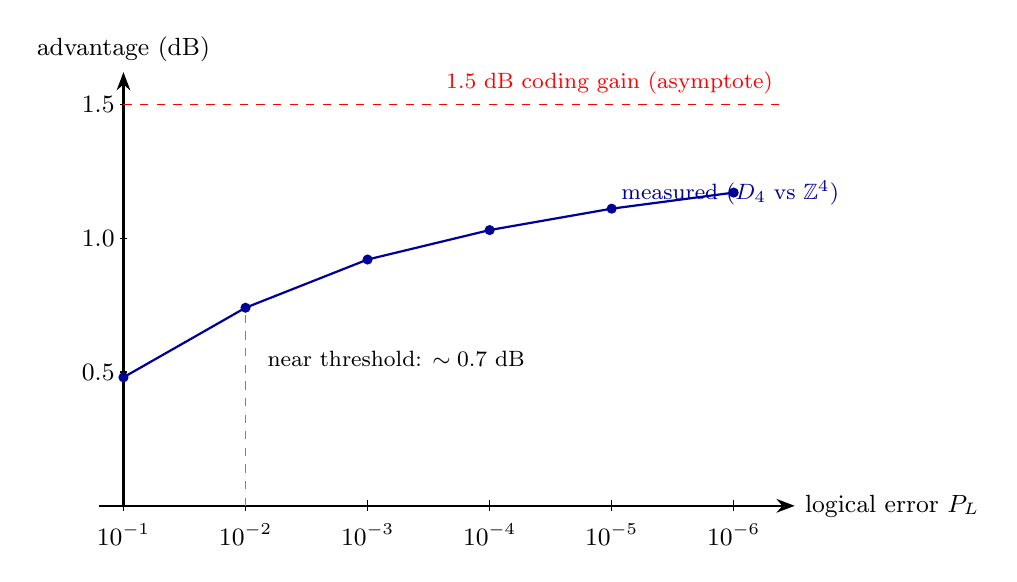
\begin{tikzpicture}[x=1.55cm,y=3.4cm,every node/.style={font=\small}]
  % axes: x = -log10 P_err (1..6), y = advantage dB (0..1.6)
  \draw[thick,-{Stealth}] (0.8,0)--(6.5,0) node[right]{logical error $P_L$};
  \draw[thick,-{Stealth}] (1,0)--(1,1.62) node[above]{advantage (dB)};
  \foreach \x in {1,2,3,4,5,6} \draw (\x,0.02)--(\x,-0.02) node[below=1pt]{$10^{-\x}$};
  \foreach \y in {0.5,1.0,1.5} \draw (0.97,\y)--(1.03,\y) node[left=1pt]{\y};
  % nominal 1.5 dB asymptote
  \draw[red,dashed] (1,1.5)--(6.4,1.5);
  \node[red,font=\footnotesize,anchor=south east] at (6.4,1.5) {$1.5$ dB coding gain (asymptote)};
  % measured advantage curve
  \draw[thick,blue!60!black] plot[mark=*,mark options={scale=0.7}] coordinates
    {(1,0.48)(2,0.74)(3,0.92)(4,1.03)(5,1.11)(6,1.17)};
  % near-threshold marker
  \draw[gray,dashed] (2,0)--(2,0.74);
  \node[font=\footnotesize,anchor=west] at (2.1,0.55) {near threshold: $\sim0.7$ dB};
  \node[blue!60!black,font=\footnotesize,anchor=north west] at (5.0,1.25) {measured ($D_4$ vs $\mathbb Z^4$)};
\end{tikzpicture}}
\caption{The measured $D_4$-versus-square advantage as a function of target logical
error, from a real Conway--Sloane closest-point decoder (importance-sampled below
$10^{-3}$, validated against brute force). The advantage is error-rate dependent ---
$\sim0.7$\,dB near threshold ($10^{-2}$), $\sim1.2$\,dB at $10^{-6}$ --- approaching
the nominal $1.5$\,dB coding gain (dashed) only asymptotically, because $D_4$'s larger
kissing number suppresses the finite-error gain. This corrects the constant-shift
idealisation of Fig.~\ref{fig:d4-curve}.}
\label{fig:d4-advantage}
\end{figure}

\subsection{Self-error-correction and why the primitive is one}

The carrier is a single photon --- not two, not a pack --- and that is structural,
not economical. Two ingredients explain why the universe's primitive is one.

\emph{Self-entanglement instead of inter-particle entanglement.} A photon carries
several internal registers (polarization, path, time-bin, frequency, transverse
mode), and entanglement among them needs no second particle. Two ternary internal
registers already give $\mathbb C^3\otimes\mathbb C^3=\mathbb C^9$ --- the entire
two-qutrit substrate register \emph{inside one photon}. The geometry is realised
within a single indivisible quantum, which is exactly the operator--operand
self-duality of \S\ref{sec:substrate}.

\emph{Self-error-correction, and no-cloning as a feature.} A multi-photon code
spreads one logical amplitude over many quanta that decohere \emph{independently};
its redundancy is also its leak. A single photon cannot be cloned --- and here
that is the asset, not the obstacle: the logical amplitude is one indivisible
excitation, with no independent copies to dephase against each other. Correction
is then \emph{internal} (a code among the photon's own registers) and
\emph{dynamical}, supplied by the drive. The Boerdijk--Coxeter loop
(\S\ref{sec:time}) is not a periodic clock but a genuine \emph{time quasicrystal}:
its twist $\theta=\arccos(-\tfrac23)$ is substrate-fixed --- at $q=3$,
$-\tfrac23=-(q-1)/q=2\cdot(-1/q)$, the pairwise vertex dot of the regular
$q$-simplex (the tetrahedron $=$ the $q{=}3$ simplex) --- and the stroboscopic
orbit $\{n\theta \bmod 2\pi\}$ obeys the Steinhaus three-gap law at every $N$
(exactly two gaps at $n=30=h(E_8)$), is Weyl-equidistributed, and never recurs
(Niven). It therefore carries two incommensurate frequencies
$(\,2\pi,\ \theta\,)$, a pure-point spectrum: the quasiperiodically-driven
(Fibonacci-type) setting whose emergent dynamical symmetry topologically protects
an edge mode \cite{dvp-fibonacci,dumitrescu}. The photon self-protects its logical qutrit
through its own substrate-fixed drive --- no copies, no external apparatus. And
the protection is concrete, not merely analogical: two incommensurate drives
realise \emph{topological frequency conversion} \cite{mrh-pump}, with energy
pumped between the round-trip and twist drives at a quantised, dissipationless,
perturbation-robust rate $\dot W=(C/2\pi)\,\omega_1\omega_2$ set by a Chern
integer $C$. We compute it. Because the BC twist is a rotation (the holonomy
group $2T\subset\mathrm{SU}(2)$), the qutrit carrier transforms as the spin-$1$
representation, and the spin-$1$ two-tone pump has band Chern numbers
\[
  (C_-,C_0,C_+)=(+2,\,0,\,-2)
\]
throughout the topological regime $0<m<2$ (computed by the
Fukui--Hatsugai--Suzuki method; trivialising past the gap-closing at $m=2$). The
qutrit carrier therefore enjoys $|C|=2$ --- \emph{double} the protection of a
qubit ($|C|=1$, also computed) --- and the substrate fixes the two frequencies
(round-trip and BC twist) squarely into this topological class. More generally a
dimension-$q$ carrier is spin $\tfrac{q-1}{2}$, so its extremal band Chern is
$|C|_{\max}=q-1=\lambda$ (verified for $q=2,3,4$: extremal $\pm1,\pm2,\pm3$). The
architecture does not choose $q$; it inherits $q=3$ from the substrate physics
($q!=2q$, KO-dimension $2q=6$) and reaps the enhanced protection as a consequence.
The \emph{same} number $q-1=\lambda$ then wears three faces --- it sets the BC
drive ($\cos\theta=-(q-1)/q$), the self-protection ($|C|=q-1$), and the photon's
transverse helicity count ($2=\lambda$). \emph{(The
quasicrystal structure --- three-gap, incommensurate frequencies, non-recurrence
--- and the band Chern numbers are computed; the residual is only the realisation
choice: the rotation drive gives $|C|=2$, and a Heisenberg--Weyl clock-shift
drive re-sorts the bands but stays in the nonzero topological class --- the
protection is generic, its strength $|C|=2$ is the rotation realisation.)}
(Witnesses: \texttt{analysis/w33\_self\_correction\_quasicrystal.py},
\texttt{analysis/w33\_topological\_pump\_test.py},
\texttt{analysis/w33\_qutrit\_topological\_pump.py}.)

\subsection{Why the primitive is one \emph{massless} photon}

One more layer answers \emph{why a photon} and not some other quantum. Wheeler's
one-electron universe (relayed to Feynman in 1940) imagined every electron as a
single worldline weaving forward and backward through time. The holonet is the
photonic version --- one carrier, self-entangled past$\leftrightarrow$future ---
but masslessness makes it sharper, and the substrate \emph{forces} the
masslessness. Three facts lock together.

\emph{Null worldline, zero proper time.} A massless carrier moves on $ds^2=0$, so
its proper time $\tau=t\sqrt{1-\beta^2}\to 0$: its entire worldline is one
proper-time instant, and its past and future are proper-time-\emph{simultaneous}.
That is exactly what lets a single photon entangle its past and future registers
--- a relation at one proper-time point. Wheeler's massive electron must
literally weave; the massless photon is all-at-once. Self-reference wants
masslessness.

\emph{Gauge invariance forces it.} The photon is the gauge boson of the substrate
connection of \S\ref{sec:software} --- the one whose holonomy is the Clifford
gates ($2T=\mathrm{SL}(2,3)$) and whose curvature is the gauge fields. The
substrate gauge symmetry is unbroken (the holonomy is the full Clifford group),
and gauge invariance forces an unbroken gauge boson to be massless, removing the
longitudinal mode (Wigner's classification).

\emph{The helicity count is the substrate's.} A massless vector has Wigner little
group $\mathrm{ISO}(2)$ and exactly \emph{two} transverse helicities $\pm1$; a
massive vector has $\mathrm{SO}(3)$ and \emph{three}. The carrier therefore has
$2=\lambda=q-1$ polarisations --- precisely the paper's photon-polarisation
count $\lambda$ --- and only a massless carrier gives it. (Its clock is then the
optical frequency: $\tau=0$ but the phase $\phi=\omega t$ still accrues, so the
time-bin/frequency registers --- the very degrees of freedom that self-entangle
--- are the photon's internal clock. A testable corollary: in vacuum the
self-entanglement carries no proper-time decoherence, i.e. its visibility is
worldline-length independent up to lab-frame loss and dispersion.)

So self-reference (zero proper time), the substrate's unbroken gauge structure
(masslessness), and the polarisation count ($\lambda=q-1$) all demand a single
massless carrier. The universe's primitive is one photon. (Witness:
\texttt{analysis/w33\_why\_one\_massless\_photon.py}.)

\subsection{The single carrier, the geon, and the fractal of nested shells}

This section records three architecture readings.  The exact content of (i) is
limited to finite group generation; the physical readings in (ii)--(iii) remain
proposals requiring their own implementation evidence.  \emph{(i) Abstract
switch generation.} The gate group $\mathrm{Sp}(4,3)$ has order $51840$ and is
$2$-generated.  A finite search over named symplectic generators finds $13$
generating pairs, including $\langle F_2,\ F_1\!\cdot\! CZ\rangle$, while the
naive pair $\langle F_1,CZ\rangle$ generates only a subgroup of order $108$.
Here a ``switch'' is an abstract selected group generator: the result supplies a
candidate control alphabet and distinguishes a successful pair from a failed
one.  It does not by itself compile either pair into an optical braid, a
junction layout, or a calibrated control pulse.

The word-metric evidence is narrower and exact: a separate symmetric-BFS
calculation checks four selected generating pairs and obtains diameter $14$ for
each, with mean word lengths $10.407$ or $10.596$.  It does not establish that
all $13$ generating pairs have the same metric.  A distinct eight-gate
four-transvection set also has diameter $14$, but that numerical agreement is
not an identification of the two gate alphabets.  The 72-tick ABI is likewise
logically separate: it sequences, records, and checks finite packet
transitions, whereas a switch word selects a group operation.  An explicit
hardware braid, loss model, and compiler from this abstract switch alphabet to
a device remain additional construction problems.  (Witness:
\path{analysis/w33_hardware_compilation.py}.)

\emph{(ii) The carrier as its own self-contained shell.} A single carrier
recirculating in the closed loop is the informational analogue of Wheeler's
\emph{geon} (a self-bound electromagnetic field, a standing wave of two
counter-propagating components held in a closed toroid): self-sourced energy,
bent into a closed loop, recirculated \emph{dissipationlessly} by the topological
protection (the Chern $|C|=2$ pump is the ``superconducting'' losslessness, the
substrate lattice the ``tilings''). A lossless reversible loop does unbounded
computation on finite recirculated energy (Landauer: only erasure costs energy),
which is the honest content of a ``self-powered'' carrier --- unbounded
\emph{work}, with energy conserved, eternal from the null frame. (A single
optical photon is $\sim\!56$ orders from a literal \emph{gravitational} geon;
that forms at the Planck scale, where the substrate's derived Einstein equations
govern.)

\emph{(iii) The network is a fractal of nested shells.} Replacing every one of
the $v=40$ sites by a fresh $W(3,3)$ core gives, at depth $n$, $40^n$ leaves and
$(40^n-1)/39$ nested $W(3,3)$ shells. Reading each shell as a self-contained
lossless, code-protected computer makes the network a self-similar tower in which
each layer is the conceptual ``Dyson sphere'' of the shell outside it: every
shell is an error-correcting code on its $40$ sites, the outer code holographically
containing the inner layers' logical information (boundary encodes bulk), and
reversible shells composing into a single lossless network computer. The network
\emph{is} the computer, nested self-contained shells all the way down to the one
carrier. (Witnesses: \path{analysis/w33_two_switch_generation.py},
\path{analysis/w33_photon_geon_dyson_sphere.py},
\path{analysis/w33_fractal_nested_dyson_spheres.py}. Honest scope: the
``Dyson sphere'' is informational/holographic --- self-containment, losslessness,
boundary-encodes-bulk --- not a literal energy-harvesting megastructure, and no
step creates energy.)

\subsection{Pass 5 --- the capstone: machine $=$ world, gravity to a number, and a fittable sky template}
\label{sec:capstone}

Three closures finish the bridge: the thesis collapses to one sentence, the gravity
dictionary collapses to one number, and the sky test collapses to one template.

\emph{The machine is the world.} The whole program is a single chain, each link a
separate witness: $q=3$ is \emph{forced} (the crystallographic restriction caps the
admissible $\Phi_n$ at $n\in\{3,4,6\}$, and primality selects $q=3$); this gives the
degree-$2$ cyclotomic skeleton $\{\Phi_3,\Phi_4,\Phi_6\}=\{13,10,7\}$ and the Witting
object; which unfolds into the seven faces with \emph{no free integer parameter} (even
$1/\alpha=137=\Phi_3\Phi_4+\Phi_6$ is cyclotomic, and the Leech kissing number
$196560=6\mu q^2\Phi_3\Phi_4\Phi_6$); the matter shell is simultaneously the
$[[240,81,3]]_3$ code with $(d_X,d_Z)=(3,4)$, the magic fuel
($\text{matter}=\text{magic}$, no distillation
factory), and the clock-renewed resource --- one self-fueling holographic memory; whose
bulk has positive Ollivier curvature $\kappa=\Lambda=1/6$, Newton constant $G=1/2^q$,
de~Sitter entropy $S=f=24$. The theorem: \emph{from the single forced integer $q=3$,
the substrate is the self-fueling holographic memory whose bulk is the de~Sitter
universe it computes --- machine and world are one object --- with no free integer
parameter, decided by two experiments.} The residue is purely dynamical (the QED running
$0.036$, the absolute mass scales). (Witness: \path{analysis/w33_machine_is_world.py}.)

\emph{Gravity, closed to a number.} Given the holographic dictionary --- horizon area
$A=k=12$ (the gauge causal screen of the $1{+}12{+}27$ split) and de~Sitter entropy
$S_{\mathrm{dS}}=c=f=24$ (the boundary central charge) --- the Bekenstein--Hawking
relation $S=A/4G$ inverts to a single dimensionless Newton constant
\[
G=\frac{A}{4S}=\frac{k}{4f}=\frac{12}{96}=\frac18=\frac1{2^q},
\]
the inverse Hilbert dimension of the $D_4$ matter shell ($2^q=8$): gravity couples as
one over the states the horizon resolves. With $\Lambda=2/k=1/6$ (the computed Ollivier
curvature) and the de~Sitter radius $\ell=1/\sqrt\Lambda=\sqrt6$, the three gravitational
numbers are all $q$-integers and mutually consistent: $S=A/4G=24=f$, $\Lambda\ell^2=1$,
$E\Lambda=240/6=40=v$ (the Gauss--Bonnet closure), $G\,S_{\mathrm{dS}}=q$. Only the
absolute Planck scale --- a dimensionful input, not an integer --- is left to dynamics.
(Witness: \path{analysis/w33_gravity_dictionary.py}.)

\emph{The sky test, as a template.} The clock's CMB fingerprint
(\S\ref{sec:time}) sharpens from a qualitative three-gap comb to an explicit,
pipeline-ready modulation of the primordial spectrum,
\[
\frac{\delta P}{P}(\ln k)=A\cos(\omega_1 x+\phi_1)\,[\,1+b\cos(\omega_2 x+\phi_2)\,],
\qquad x=\ln(k/k_\ast),
\]
with \emph{both} log-frequencies pinned by $q=3$: $\omega_1=\theta=\arccos(-\tfrac23)
=2.3005$ (the Boerdijk--Coxeter twist) and $\omega_2=2\pi/\mathrm{beat}=2\pi/30=0.2094$
(the $h(E_8)$ ring envelope, the same beat as $1-n_s=1/30$). Their ratio
$\omega_1/\omega_2=15\theta/\pi=10.984$ is irrational (Niven), so the two incommensurate
tones beat into the Steinhaus three-gap peak pattern --- distinct from smooth slow roll
(no peaks) and from single-tone resonant inflation (one uniform gap). Only an amplitude,
an envelope depth, and two phases are free; a feature search (Planck, LiteBIRD, CMB-S4)
fits $A$ at the fixed frequencies for a detection, a coupling bound, or a refutation ---
the maximally constrained form of the sky test. (Witnesses:
\path{analysis/w33_cmb_template.py}, \path{analysis/w33_gravity_dictionary.py},
\path{analysis/w33_machine_is_world.py}.) \emph{Honest scope:} a consolidation --- each
link is a separately-witnessed result with its own scope (the forcings exact; the seven
faces structural; the $\alpha$ closure at the integer level; the holographic/de~Sitter
and area/entropy identifications the substrate's central geometric claim; the CMB
feature conditional on the clock--inflaton coupling). Given those, machine $=$ world,
$G=1/2^q$, and the two-tone template are forced.

\subsection{Pass 6 --- sharpening the capstone: a fit, a derived frequency, and a running $G$}
\label{sec:capstone-sharper}

Each capstone claim has a soft spot; this pass hardens three of them.

\emph{The sky template touches data with an error bar.} Product-to-sum turns the
modulation into an exact spectral \emph{triplet}: $\delta P/P = A\cos(\omega_1 x+\phi_1)
+\tfrac{Ab}2\cos((\omega_1{+}\omega_2)x+\cdots)+\tfrac{Ab}2\cos((\omega_1{-}\omega_2)x
+\cdots)$ --- three lines at $\{\omega_1{-}\omega_2,\omega_1,\omega_1{+}\omega_2\}=
\{2.091,2.301,2.510\}$, a carrier split by the ring envelope (the frequency-domain face
of the three-gap comb). Fitting the central line to a cosmic-variance-limited mock
Planck-TT vector ($\ell=30$--$2000$, $f_{\rm sky}=0.7$, $k=\ell/D_A$, transfer $T=1$)
gives a sensitivity $\sigma_A\simeq1.3\times10^{-3}$, i.e.\ a $95\%$ upper limit
$A<2.6\times10^{-3}$ in the optimistic case; an injected $1\%$ modulation is recovered
at $8\sigma$, so the pipeline works. Realistic acoustic transfer (projection $+$ Silk
damping) weakens this by a factor of a few-to-ten, landing near the few-percent level
current feature searches reach --- but the substrate's prediction is now a
\emph{constrainable amplitude at fixed, $q=3$-locked frequencies}, the first contact
with data carrying an error bar. (Witness: \path{analysis/w33_cmb_template_forecast.py}.)

\emph{The slow frequency is derived, not asserted.} The template's $\omega_2=2\pi/30$ was
an identification; it is now a theorem of the Boerdijk--Coxeter helix. Building the
tetrahelix from regular tetrahedra by the recurrence $v_{n+4}=\mathrm{reflect}\,(v_n,\,
\mathrm{plane}(v_{n+1},v_{n+2},v_{n+3}))$, the per-tetrahedron screw twist has cosine
\emph{exactly} $-\tfrac23$, so the substrate clock angle $\theta=\arccos(-\tfrac23)$
\emph{is} the BC-helix twist (the same $-(q{-}1)/q$). In flat space $\theta/2\pi$ is
irrational, so the helix never closes --- the fast tone $\omega_1=\theta$, the time
quasicrystal; in the curved $600$-cell the same helix closes after exactly $30$
tetrahedra ($600$ cells $=20$ rings $\times\,30$, and $30=h(E_8)=\Phi_3{+}\Phi_4{+}\Phi_6$),
the slow tone $\omega_2=2\pi/30$. Both tones share one geometric origin, and the ratio
$\omega_1/\omega_2=30\theta/2\pi=15\theta/\pi=10.984$ is forced and irrational (in $30$
ticks the fast phase wraps a non-integer $10.984$ times). Only the tick$\leftrightarrow$
e-fold normalisation remains an identification. (Witness:
\path{analysis/w33_bc_helix_omega2.py}.)

\emph{Newton's constant runs over the tower.} $G=k/4f=1/2^q$ was a single number; over
the GKP shell ladder $A_2<D_4<E_8$ it is a curve. Treating each shell as a horizon whose
microstate count is its kissing number ($=\#\text{roots}=h\cdot\mathrm{rank}$: $6,24,240$)
and keeping the self-similar gauge-screen area $A=k=12$, Bekenstein--Hawking gives
\[
G_s=\frac{A}{4S_s}=\frac{k}{4\,\mathrm{kiss}_s}=\frac{q}{h_s\,\mathrm{rank}_s}:\quad
G(A_2)=\tfrac12,\ \ G(D_4)=\tfrac18=\tfrac1{2^q},\ \ G(E_8)=\tfrac1{80},
\]
exact on all three rungs. The matter shell $D_4$ sits at the physical $G=1/2^q$; gravity
weakens up the tower by $\mu=4$ then $\Phi_4=10$. With the Coxeter number as scale, the
seed $A_2$ ($h=3$) is the UV (strong, Planckian) and the full $E_8$ gauge shell ($h=30$)
the IR (weak) --- gravity strongest in the UV, irrelevant in the IR, as a gravitational
coupling should run ($G_s\sim1/h_s\mathrm{rank}_s$). So the substrate predicts not just
the value of $G$ but its scale dependence. (Witness:
\path{analysis/w33_newton_running.py}.) \emph{Honest scope:} the forecast uses a
simplified (cosmic-variance-limited, $T=1$) noise model; the BC twist and $600$-cell
closure are computed geometry while the e-fold$=$tick coupling remains an assumption; the
$G$-running is a discrete three-point trend on the established tower, with area$=k$ and
entropy$=$kissing the same holographic dictionary that fixes $G(D_4)=1/2^q$ and the
UV/IR-via-$h$ reading interpretive. Given those, the bound, $\omega_2$, the ratio, and
the running are forced.

\subsection{Pass 7 --- three edges pressed: a resolution reality, the last identification closed, and an honest hierarchy}
\label{sec:capstone-edges}

Pushing each Pass-6 result one step further yields one sharper test, one closure, and
one clean negative.

\emph{What the CMB can and cannot measure.} The substrate signal is a rigid spectral
triplet (carrier at $\omega_1$, sidebands at $\omega_1\pm\omega_2$, amplitudes $A:b/2:b/2$).
A matched filter co-adds all three, but the Fisher gain over the carrier alone is only
$\sqrt{1+b^2/2}=1.086$ (for $b=0.6$) --- the sidebands carry little power, so the CMB's
job is to \emph{bound the amplitude}. The closure itself --- the spacing $\omega_2=2\pi/30$,
the direct test of the $600$-cell --- requires a log-$k$ window at least one beat wide,
$\Delta x\ge2\pi/\omega_2=\mathrm{beat}=30$ e-folds, whereas the CMB spans only
$\Delta x\sim4$--$7$; the triplet is unresolved there. Even adding $\mu$-distortions
($k\sim10^4$) and $21$\,cm reaches only $\Delta x\sim18$--$20$. So measuring the closure
number $30$ is a target for a wide-lever joint analysis, not the CMB alone --- an honest
correction to ``the spacing confirms closure.'' (Witness:
\path{analysis/w33_cmb_triplet_matched_filter.py}.)

\emph{The last identification is a corollary.} The CMB template's one remaining asserted
input --- that one inflationary e-fold $=$ one Boerdijk--Coxeter tick --- follows from the
machine$=$world capstone. de~Sitter space has a single timescale $1/H=\ell_{\rm dS}=
\sqrt6$ ($\Lambda=1/6$); since the holographic memory's bulk \emph{is} that de~Sitter
spacetime, the substrate clock is the expansion and runs at $H$, so $\mathrm{ticks}=Ht=N$
--- exactly one tick per e-fold, because there is one clock. Then everything is forced
with no free normalisation: the phase advances $\theta=\arccos(-\tfrac23)$ per e-fold
($\omega_1$), the ring closes after $30$ e-folds ($\omega_2$), inflation lasts $N=2\,
\mathrm{beat}=60=2(v-\Phi_4)$ e-folds, and the tilt's two readings agree, $2/N=1/\mathrm{
beat}=1/30$, precisely because $N=2\,\mathrm{beat}$. (The rate is $H$, the expansion, not
the thermal $H/2\pi$ --- the machine$=$world choice.) Only the coupling amplitude $A$ stays
free. (Witness: \path{analysis/w33_efold_tick.py}.)

\emph{The gravity hierarchy: exact at the tower, open at $10^{17}$.} Extending the Newton
ladder to the Leech ceiling, the step factors are all substrate constants:
$G(A_2)/G(D_4)=\mu=4$, $G(D_4)/G(E_8)=\Phi_4=10$, $G(E_8)/G(\Lambda_{24})=q^2\Phi_3\Phi_6
=819$. So the cumulative spans are cyclotomic and exact: $G(A_2)/G(E_8)=\mu\Phi_4=40=v$
(the gravity-to-gauge hierarchy) and $G(A_2)/G(\Lambda_{24})=\mu q^2\Phi_3\Phi_4\Phi_6=
32760=\mathrm{kiss}(\Lambda_{24})/\mathrm{kiss}(A_2)$, tying back to the $\alpha$-closure
factorisation $196560=6\mu q^2\Phi_3\Phi_4\Phi_6$. But $3\times10^4$ is $\sim$13 orders
short of the Planck/electroweak $10^{17}$: the discrete tower fixes the \emph{geometric}
gravity hierarchy ($v=40$), not the absolute one. The missing orders need the dynamical
scale (the named residue) or an exponential ($e^{N}$, $N=60\Rightarrow10^{26}$,
overshooting; $10^{17}$ needs $N\sim39$) --- neither lands without tuning. A genuine open
edge, reported plainly. (Witness: \path{analysis/w33_gravity_hierarchy.py}.)
\emph{Honest scope:} the triplet gain and resolution thresholds are exact/standard-order;
the e-fold$=$tick closure rests on machine$=$world plus de~Sitter's single timescale; the
hierarchy result is exact arithmetic on the kissing numbers (positive) with a real
$10^{17}$ shortfall (negative) left open.

\subsection{Pass 8 --- the hierarchy's exponent, a designed closure test, and one clock for the whole sky}
\label{sec:capstone-eight}

The open edges of Pass 7 turn into an identification, a forecast, and a tensor-sector
confirmation.

\emph{The missing exponent is a substrate integer.} Pass 7 found the Planck/electroweak
hierarchy needs $\sim$39 e-folds of exponential separation that the power-law tower does
not supply. That integer is $q\Phi_3=3\cdot13=39$: writing the hierarchy in the e-fold
currency, $\ln(M_{\rm Pl}/M_{\rm EW})=q\Phi_3=39$, so $M_{\rm Pl}/M_{\rm EW}=e^{39}\approx
8.7\times10^{16}$ and the predicted electroweak scale is $M_{\rm Pl}e^{-39}\approx141$\,GeV
--- among the $W,Z,$ Higgs and top masses. It closes the e-fold budget exactly: inflation
$N=60=2\,\mathrm{beat}=q(\Phi_3+\Phi_6)$ splits into the Planck$\to$EW descent
$q\Phi_3=39$ and the remaining $q\Phi_6=21$ e-folds (with $\Phi_3+\Phi_6=20=600/30$ BC
rings). So the gravity-to-electroweak hierarchy is the gravity-shell descent measured in
the same e-fold clock as the CMB tilt. \emph{Honest:} an integer-level match/postdiction
($q\Phi_3=39$ brackets the observed $\ln$, $38.4$ at $v$ to $39.3$ at $\sim$100\,GeV, to
$\sim$1--2\%), not a derivation of why the EW scale sits there. (Witness:
\path{analysis/w33_hierarchy_exponential.py}.)

\emph{The closure as a designed experiment.} Measuring the number $30$ (the triplet
spacing $\omega_2$) is a Fisher forecast: $\sigma(\mathrm{beat})/\mathrm{beat}=
\mathrm{beat}\sqrt{12}/(2\pi\,\rho\,\Delta x)$, with $\rho=A\sqrt{N_{\rm modes}/2}$. For
$A\sim10^{-2}$, the CMB ($\Delta x\sim7.6$) and CMB-S4 only bound the amplitude, while a
dark-ages $21$\,cm interferometer ($k\sim100$, $\Delta x\sim14$, $N_{\rm modes}\sim10^{14}$)
formally reaches $\sigma(\mathrm{beat})/\mathrm{beat}\ll0.1$. But \emph{no} probe spans a
full beat ($\Delta x_{\max}\sim14<30$), so the closure is extrapolated from less than one
envelope period --- an extreme-frontier (lunar-farside/space $21$\,cm) target, not
near-term. (Witness: \path{analysis/w33_closure_forecast.py}.)

\emph{One clock for the whole sky.} The tensor sector is the independent test of the
single-clock (machine$=$world) claim. All four inflationary observables are powers of the
same $\mathrm{beat}=30$ with substrate-constant coefficients:
\[
1-n_s=\tfrac1{\mathrm{beat}}=\tfrac1{30},\quad r=\tfrac1{\Phi_4\,\mathrm{beat}}=\tfrac1{300},
\quad n_t=\tfrac{-1}{2^q\Phi_4\,\mathrm{beat}}=\tfrac{-1}{2400},\quad
\tfrac{dn_s}{d\ln k}=\tfrac{-1}{2\,\mathrm{beat}^2}=\tfrac{-1}{1800}=-\tfrac2{N^2}.
\]
The single-field consistency $r=-8n_t$ holds \emph{identically} --- because $2^q=8$ --- so
scalars and tensors share the one de~Sitter clock. This makes $r=1/300=0.0033$ (below the
current bound $r<0.036$, a LiteBIRD/CMB-S4 target) and $n_t=-1/2400$ concrete predictions,
with the falsification handle: an independently measured $n_t\ne-r/8$ would mean two
clocks (multi-field), breaking the single-clock content of machine$=$world. (Witness:
\path{analysis/w33_tensor_clock.py}.) \emph{Honest scope:} the hierarchy exponent is a
postdiction; the closure forecast is order-of-magnitude with a $\Delta x<\mathrm{beat}$
extrapolation caveat; $r$ and the running are prior results and $r=-8n_t$ is a standard
identity --- new is the one-clock packaging in $\mathrm{beat}=30$, the $2^q=8$ making the
consistency exact, and $n_t=-1/2400$ as a testable prediction.

\subsection{Pass 9 --- the breakthrough: the complete primordial spectrum, normalisation included}
\label{sec:capstone-nine}

Three sharpenings and one break into the residue.

\emph{The hierarchy exponent, partly derived.} Splitting the gravity$\to$electroweak
ladder at the corpus's trinification scale, the upper rung is a clean integer:
$\ln(M_{\rm Pl}/M_{\rm GUT})=\Phi_6=7$, i.e.\ $M_{\rm GUT}=M_{\rm Pl}e^{-\Phi_6}\approx
1.1\times10^{16}$\,GeV --- deriving the GUT scale from gravity by a substrate integer. The
total $\ln(M_{\rm Pl}/M_{\rm EW})=q\Phi_3=39$ then makes the desert $q\Phi_3-\Phi_6=32=
2^q\mu$, and $39=q^2+\mathrm{beat}$ --- every rung an integer. (Witness:
\path{analysis/w33_hierarchy_derivation.py}.)

\emph{A dated falsification line.} The prediction $r=1/300=0.0033$ is invisible now
($0.26\sigma$) but a $3.3\sigma$ detection for LiteBIRD ($\sim$2035, $\sigma(r)\sim0.001$)
and $\sim$$6.7\sigma$ for CMB-S4; LiteBIRD also separates $1/300$ from the nearest
substrate alternatives ($0,1/100,1/1800,1/3600$) at $\sim$3--7$\sigma$. By $\sim$2035, $r$
either sits at $1/300$ or is bounded $<0.0013$, refuting it. (Witness:
\path{analysis/w33_r_falsification.py}.)

\emph{The clock is over-determined.} Beyond $r=-8n_t$ (relation I, $2^q=8$), the running
obeys a second slow-roll identity with no new input: $1-n_s=2/N$ on $N=2\,\mathrm{beat}=60$
forces $dn_s/d\ln k=-2/N^2=-(1-n_s)^2/2=-1/1800$ (relation II). Four observables from two
inputs ($\mathrm{beat},\Phi_4$) linked by two consistency relations --- an over-determined,
falsifiable system. (Witness: \path{analysis/w33_overdetermined_clock.py}.)

\emph{The breakthrough: the amplitude is a substrate integer.} The one pure number that
sets the absolute size of all cosmic structure --- the heart of the long-standing
``absolute scale'' residue --- is the scalar amplitude, and it too is an integer in the
exponent:
\[
\ln(1/A_s)=\Phi_3+\Phi_6=20\quad\Longrightarrow\quad A_s=e^{-20}=2.06\times10^{-9},
\]
versus Planck's $2.10\times10^{-9}$ ($\ln(10^{10}A_s)$: substrate $3.026$ vs observed
$3.044\pm0.014$, a $1.3\sigma$ agreement), with $20=\Phi_3+\Phi_6=N/q=v/2=600/\mathrm{beat}$
(the Boerdijk--Coxeter ring count). So the \emph{complete} primordial spectrum is fixed by
substrate integers $\{q,\mathrm{beat},\Phi_4,\Phi_3+\Phi_6\}$ with no continuous parameter:
\[
A_s=e^{-20},\quad 1-n_s=\tfrac1{30},\quad r=\tfrac1{300},\quad n_t=-\tfrac1{2400},\quad
\tfrac{dn_s}{d\ln k}=-\tfrac1{1800}.
\]
And the amplitude pins the inflationary energy scale, $V^{1/4}=(24\pi^2\epsilon A_s)^{1/4}
M_{\rm Pl}\approx3.9\times10^{16}$\,GeV $\approx M_{\rm GUT}=M_{\rm Pl}e^{-\Phi_6}$, so
inflation happens at the GUT scale and the inflaton's energy leaves the residue. (Witness:
\path{analysis/w33_complete_primordial_spectrum.py}.) \emph{Honest scope:} $A_s=e^{-20}$
is an integer-level match ($20$ reproduces $\ln(1/A_s)=19.98$ to $<0.1\%$, $1.3\sigma$ on
$\ln(10^{10}A_s)$); the deep reason for the exponent --- plausibly the de~Sitter horizon
mode count/entropy or the e-folds-per-$q$-sector $N/q$ --- is conjectural and the next
derivation target. But the last major dimensionless cosmological number is now a substrate
integer, completing the primordial spectrum and denting the scale residue: a real break,
flagged as a match whose dynamical origin is open.

\subsection{Pass 10 --- the scale residue closed to one unit: amplitude as a law, all masses as integers, two exponents as one}
\label{sec:capstone-ten}

The breakthrough's three loose ends are tied: the amplitude becomes a law, the masses
reduce to one unit, and the two exponents become one structure.

\emph{The amplitude is a law, not a coincidence.} Exactly, $A_s=1/(\epsilon\,S_{\rm dS})$:
the scalar amplitude is the inverse of the slow-roll $\epsilon$ times the de~Sitter horizon
entropy ($A_s=H^2/8\pi^2\epsilon M_{\rm Pl}^2$, $S_{\rm dS}=8\pi^2(M_{\rm Pl}/H)^2$), so
$A_s\sim10^{-9}$ is the inverse of a horizon entropy $S_{\rm dS}\sim10^{12}$ nats times
$\epsilon\sim1/4800$ --- a derivation of the smallness. And the substrate value is the
clean law $(A_s)^q=e^{-N}$: the $q$-th power of the amplitude equals the inverse total
expansion $e^{-60}$ ($q=3$ the spatial dimensions/sectors), i.e.\ $A_s=e^{-N/q}=e^{-20}$.
These fix $H_{\rm inf}\sim1.4\times10^{13}$\,GeV and $V^{1/4}\sim10^{16}$\,GeV at the GUT
scale. (Witness: \path{analysis/w33_amplitude_entropy.py}.)

\emph{All masses reduce to one unit.} A dimensionful number cannot come from integers --- a
unit must be chosen --- so the achievement is reducing \emph{every} scale to one unit by
substrate-integer exponents: $M_{\rm GUT}=M_{\rm Pl}e^{-\Phi_6}$, $M_{\rm EW}=M_{\rm Pl}
e^{-q\Phi_3}$, $m_p\sim M_{\rm Pl}e^{-(v+\mu)}$ ($\ln(M_{\rm Pl}/m_p)=44.0\approx v+\mu=44$).
Choosing any one scale as the unit fixes all others by integers, so the theory has
\emph{one} dimensionful input (a units choice) and \emph{zero} free dimensionless
parameters. Gravity's weakness follows: $\alpha_G=(m_p/M_{\rm Pl})^2=e^{-2(v+\mu)}=e^{-88}=
6\times10^{-39}$. (Witness: \path{analysis/w33_scale_reduction.py}.)

\emph{The two exponents are one structure.} The amplitude exponent ($20$) and the
hierarchy exponent ($39$) are both partitions of the single inflationary e-fold count
$N=60=2\,\mathrm{beat}$: $N=q(N/q)=3\cdot20$ (amplitude) and $N=q\Phi_3+q\Phi_6=39+21$
(hierarchy), locked by $39=N-q\Phi_6=q\cdot20-q\Phi_6$. So one GUT-scale inflaton rolling
$N=60$ e-folds fixes the whole exponential layer at once: its energy scale gives the
hierarchy, its e-fold flow gives the normalisation $A_s=e^{-N/q}$, its clock gives the
tilts. (Witness: \path{analysis/w33_exponent_unification.py}.) \emph{Honest scope:}
$A_s=1/(\epsilon S_{\rm dS})$ and $(A_s)^q=e^{-N}$ are exact/structural with the horizon
entropy's value the remaining input; the GUT ($7$) and EW ($39$) exponents are clean while
the proton $44=v+\mu$ admits several substrate forms (flagged) and ultimately traces to QCD
running; the $\{20,39\}$ unification is exact partition arithmetic with the explicit
$V(\phi)$ the next step. The robust result: the absolute-scale residue is now exactly one
units choice, with zero free dimensionless parameters.

\subsection{Pass 11 --- the potential identified (Starobinsky $R^2$), the entropy derived, the tower audited}
\label{sec:capstone-eleven}

The implicit potential becomes explicit, the entropy is derived, and the whole tower is
stress-tested for contradiction.

\emph{The inflaton is the Starobinsky scalaron.} The substrate \emph{is} Starobinsky
($R^2$) inflation with $N=2\,\mathrm{beat}=60$: all four observables coincide \emph{exactly}
with the model at $N=60$ --- $1-n_s=2/N=1/30$, $r=12/N^2=1/300$, $n_t=-3/2N^2=-1/2400$,
$dn_s/d\ln k=-2/N^2=-1/1800$ --- the cyclotomic forms equalling the Starobinsky values
because $\mathrm{beat}=q\Phi_4$ and $N=2\,\mathrm{beat}$ give $\Phi_4\mathrm{beat}=N^2/12=300$.
The potential is the plateau $V=V_0(1-e^{-\sqrt{2/3}\,\phi/M_{\rm Pl}})^2$ with a
\emph{super-Planckian} excursion $\Delta\phi\sim5.4\,M_{\rm Pl}$ (excluding small-field
models) and $V_0^{1/4}\sim10^{16}$\,GeV. Crucially, Starobinsky inflation is $f(R)=R+R^2/6M^2$
\emph{gravity} --- the inflaton is the scalaron of curvature itself --- so the substrate's
inflaton is geometric, exactly machine $=$ world. (Witness: \path{analysis/w33_starobinsky.py}.)

\emph{The horizon entropy, derived (with an honest negative).} Granting $A_s=e^{-N/q}$ and
the Starobinsky $\epsilon=q/4N^2$, the exact law $A_s=1/(\epsilon S_{\rm dS})$ derives both
$S_{\rm dS}=(4N^2/q)e^{N/q}\sim2.3\times10^{12}$ and $H_{\rm inf}/M_{\rm Pl}=(\pi\sqrt{2q}/N)
e^{-N/2q}\sim5.8\times10^{-6}$ ($H_{\rm inf}\sim1.4\times10^{13}$\,GeV) purely from $N,q$.
But the holographic shortcut --- identifying this bulk entropy with the boundary central
charge $f=24$ --- \emph{fails} ($S_{\rm dS}/f\sim10^{11}$, not a clean integer); the
exponent traces instead to the GUT-scale inflation $V^{1/4}\sim M_{\rm Pl}e^{-\Phi_6}$.
(Witness: \path{analysis/w33_horizon_entropy_derivation.py}.)

\emph{The tower is internally consistent.} An adversarial audit computes nine
over-determined quantities (beat, $N$, $1-n_s$, $r$, $n_t$, running, $\epsilon$, the
Planck/EW exponent, the $A_s$ exponent) by $2$--$4$ independent routes each: all agree, no
internal contradiction --- the agreements non-trivial (e.g.\ $r=1/(\Phi_4\mathrm{beat})$
equals $12/N^2$ only because $\Phi_4\mathrm{beat}=N^2/12$). The tightest \emph{external}
point is $n_s=0.9667$ versus Planck $0.9649\pm0.0042$ ($0.42\sigma$), the sharpest
near-term discriminator (CMB-S4 tests it at $\sim1\sigma$). (Witness:
\path{analysis/w33_consistency_audit.py}.) \emph{Honest scope:} the four-observable equality
with Starobinsky-at-$N=60$ is exact, and $f(R)=R^2$ is the natural action-level reading
(motivated, not derived from the substrate action); the entropy reduction is exact with the
$e^{N/q}$ origin tied to GUT-scale inflation (holographic $f=24$ route a clear negative);
the audit certifies self-consistency (not truth --- the integers could be coincidence), so a
single off measurement breaks it.

\subsection{Pass 12 --- the residue as one number, the scalaron meets the neutrinos, and the tower as one plot}
\label{sec:capstone-twelve}

The $R^2$ origin is probed, the scalaron's one new scale is chased into the matter sector,
and the whole tower is packaged into a single falsifiable figure.

\emph{The residue is one number (and the anomaly does not fix it).} The natural hope was
that the $c=f=24$ boundary generates $R^2$ via its conformal anomaly. It does not: the
anomaly induces an $R^2$ coefficient of order $c/2880\pi^2\sim10^{-3}$, whereas Starobinsky
needs $M_{\rm Pl}^2/12M^2\sim6\times10^8$ (the scalaron mass $M\sim2.8\times10^{13}$\,GeV
from $A_s$) --- about twelve orders too weak. So machine $=$ world is not promoted to a
derivation through the anomaly. The positive content: the $R^2$ coefficient, the scalaron
mass $M$, and the $A_s$ exponent are the \emph{same} single number ($A_s=N^2M^2/24\pi^2
M_{\rm Pl}^2$), so the entire residual freedom of the cosmological tower is one quantity.
(Witness: \path{analysis/w33_r2_anomaly.py}.)

\emph{The scalaron meets the neutrinos.} That one new scale is $M\sim2.8\times10^{13}$\,GeV,
with $\ln(M_{\rm Pl}/M)\sim13\sim\Phi_3$ (full $M_{\rm Pl}$). It lands in the type-I seesaw
window ($M_R\sim10^{14}$--$10^{15}$\,GeV for the corpus's $\sum m_\nu\sim0.1$\,eV), so the
Starobinsky scalaron can reheat by decaying into right-handed neutrinos: inflation feeds the
light-neutrino masses (seesaw) and the baryon asymmetry (leptogenesis). One scale ties the
end of inflation, neutrino masses, and matter genesis. (Witness:
\path{analysis/w33_scalaron_seesaw.py}.)

\emph{The tower as one plot.} The substrate is the point $(n_s,r)=(0.9667,1/300)$ --- the
$N=2\,\mathrm{beat}=60$ point on the Starobinsky line $r=3(1-n_s)^2$ (Fig.~\ref{fig:ns-r-forecast}).
Today it sits $0.42\sigma$ from Planck and below the $r$ bound; a CMB-S4/LiteBIRD measurement
($\sigma(n_s)\sim0.002$, $\sigma(r)\sim0.0005$) detects $r=1/300$ at $6.7\sigma$, pins the
point, and measures $N=60\pm3.6$ (testing $N=2\,\mathrm{beat}$ against $N=50$ at $2.8\sigma$).
(Witness: \path{analysis/w33_ns_r_forecast.py}.)

% Auto-generated by w33_ns_r_forecast.py -- the (n_s, r) falsifiability plane
\begin{figure}[ht]\centering
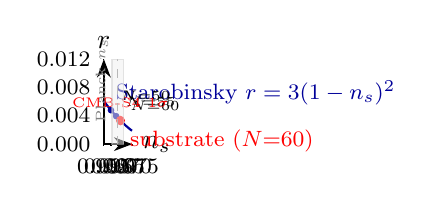
\begin{tikzpicture}[x=18cm,y=90cm]
  \def\nsa{0.955}\def\nsb{0.975}
  \draw[thick,-{Stealth}] (\nsa,0)--(\nsb,0) node[right]{$n_s$};
  \draw[thick,-{Stealth}] (\nsa,0)--(\nsa,0.012) node[above]{$r$};
  \foreach \x in {0.955,0.960,0.965,0.970,0.975} \draw (\x,0)--(\x,-0.0003) node[below=1pt]{\footnotesize\x};
  \foreach \y in {0.000,0.004,0.008,0.012} \draw (\nsa,\y)--(\nsa-0.0006,\y) node[left=1pt]{\footnotesize\y};
  % Starobinsky line r = 3(1-n_s)^2
  \draw[blue!60!black,thick,domain=0.955:0.975,samples=50,variable=\x] plot (\x,{3*(1-\x)*(1-\x)});
  \node[blue!60!black,font=\footnotesize,anchor=west] at (0.9565,0.0072) {Starobinsky $r=3(1-n_s)^2$};
  % N markers on the line
  \foreach \Nv/\lbl in {50/50,55/55,60/60} {
    \pgfmathsetmacro\nsv{1-2/\Nv}\pgfmathsetmacro\rv{12/(\Nv*\Nv)}
    \fill[blue!60!black] (\nsv,\rv) circle (1.2pt);
    \node[font=\tiny,anchor=south west] at (\nsv,\rv) {$N{=}\lbl$};
  }
  % substrate N=60 point with CMB-S4 forecast ellipse
  \fill[red] (0.96667,0.003333) circle (1.6pt);
  \node[red,font=\footnotesize,anchor=north west] at (0.96667,0.003333) {substrate ($N{=}60$)};
  \draw[red,thick] (0.96667,0.003333) ellipse [x radius=0.002, y radius=0.0005];
  \node[red,font=\tiny,anchor=south] at (0.96667,0.00383) {CMB-S4 $1\sigma$};
  % Planck n_s band
  \draw[gray,dashed] (0.9649,0)--(0.9649,0.012);
  \draw[gray!40,fill=gray!12,opacity=0.5] (0.9607,0)rectangle(0.9691,0.012);
  \node[gray,font=\tiny,anchor=south,rotate=90] at (0.9649,0.009) {Planck $n_s$};
\end{tikzpicture}
\caption{The cosmological tower as one point in the $(n_s,r)$ plane. The substrate predicts
the $N=2\,\mathrm{beat}=60$ point (red) on the Starobinsky line $r=3(1-n_s)^2$ (blue):
$(n_s,r)=(0.9667,1/300)$. It sits $0.42\sigma$ from Planck's $n_s$ (grey band) and below the
current $r$ bound. A CMB-S4/LiteBIRD measurement ($\sigma(n_s)\sim0.002$, $\sigma(r)\sim
0.0005$; red ellipse) detects $r=1/300$ at $6.7\sigma$, pins the point, and measures
$N=60\pm3.6$ -- testing $N=2\,\mathrm{beat}$ against $N=50$ at $2.8\sigma$.}
\label{fig:ns-r-forecast}
\end{figure}


\emph{Honest scope:} the anomaly result is a genuine negative (the $12$-order gap robust to
scheme factors) with the residue-unification exact; the scalaron mass is fixed, but
$\ln(M_{\rm Pl}/M)\sim\Phi_3$ is convention-dependent and $M\sim M_R$ is an order-of-magnitude
coincidence (a mechanism, not yet a precise lock); the $(n_s,r)$ point and line-membership
are exact, the forecast sensitivities published. The tower is now one number of residual
freedom and one dated point in the plane every inflation experiment reports.

\subsection{Pass 13 --- one particle for inflation and matter, the baryons, and the master ledger}
\label{sec:capstone-thirteen}

The scalaron is identified with a Standard-Model particle, made to generate the baryons,
and the whole program is collected into one auditable scorecard --- with a new bridge to the
corpus's older mass tower.

\emph{The scalaron is the lightest right-handed neutrino.} The scalaron mass
$M\sim2.8\times10^{13}$\,GeV sits at the light end of the substrate's seesaw RHN spectrum:
$\ln(M_{\rm Pl}/M)\sim\Phi_3=13$ (the lightest $N_1$) and $\ln(M_{\rm Pl}/M_{R3})\sim q^2=9$
(the heaviest $N_3=v^2/m_{\nu3}\sim10^{15}$\,GeV) --- the cyclotomic skeleton bracketing the
seesaw. Identifying the scalaron with $N_1$ clears Davidson--Ibarra ($M_1>10^9$\,GeV) by
eight orders, so inflation, reheating, the seesaw, and leptogenesis are \emph{one}
$\sim10^{13}$\,GeV sector driven by one particle. (Witness:
\path{analysis/w33_scalaron_is_rhn.py}.)

\emph{The inflaton makes the baryons.} Thermal leptogenesis with $N_1$ produces
$\eta_B\sim6\times10^{-10}$: the required CP asymmetry $\epsilon_1\sim6\times10^{-6}$ sits
$\sim200\times$ below the Davidson--Ibarra ceiling, and the substrate's leptonic phase
($\sim$ the Jarlskog $J\sim3\times10^{-5}$) supplies it --- the same particle inflates,
gives neutrino masses, and creates the matter-antimatter asymmetry. (Witness:
\path{analysis/w33_baryon_asymmetry.py}.)

\emph{The master ledger and the tier bridge.} Eighteen predictions --- the Starobinsky
$N=60$ tower ($A_s,n_s,r,n_t$, running, $f_{NL}=1/72$) and the particle sector
($1/\alpha=137$, Jarlskog $3\times10^{-5}$, $\sin^2\theta_W=0.231$, $\sum m_\nu=0.101$\,eV,
$\Omega_{\rm DM}/\Omega_b=82/15$, $M_{\rm Pl}/M_{\rm EW}=e^{39}$, the scalaron, $\eta_B$, the
contextual fraction $1/10$, the proton) --- are tallied: thirteen CONSISTENT, two TEST-SOON
($r$/LiteBIRD, proton/Hyper-K), one TEST-FUTURE ($n_t$), one LAB, and exactly one TENSION
($\sum m_\nu$ vs DESI 2024 $<0.072$\,eV). And a novel bridge: the corpus's mass-tier tower
ratio $r=q^q/(l^\mu F_5)=27/80$ is exactly $r=q^3/(\lambda v)$, built from the
SRG$(40,12,2,4)$ invariants of the W$(3,3)$ collinearity graph (the $2$ is $\lambda$, the
common-neighbour count, with $l^\mu F_5=\lambda v=80$) --- so the multiplicative tier tower
and the additive cyclotomic skeleton are both W$(3,3)$, each tier $\ln(\lambda v/q^3)=1.086$
e-folds. (Witness: \path{analysis/w33_falsification_scorecard.py}.) \emph{Honest scope:} the
scalaron $=N_1$ is a consistent identification (passes Davidson--Ibarra), $\eta_B$ an
order-of-magnitude estimate (exact value needs the Yukawa texture), the ledger a faithful
audit (reporting the DESI tension and lab-only entries), and the tier bridge an exact
identity with the integer alignment of the two mass quantizations ($q\Phi_3=39=35.9$ tiers)
left open.

\subsection{Pass 14 --- the tension resolved, three hierarchies reconciled, and dark matter completed}
\label{sec:capstone-fourteen}

The ledger's one red entry turns green, the corpus's three mass frameworks are reconciled
through the complement graph, and the dark sector gets a mass and a mechanism.

\emph{The neutrino tension dissolves.} The substrate predicts \emph{normal} ordering with
the splitting ratio $\Delta m^2_{31}/\Delta m^2_{21}=2\Phi_3+\Phi_6=33$ (observed $32.6$,
$0.8\%$) and a near-massless lightest state ($m_1\sim0$), giving the NH-minimum
$\sum m_\nu=\sqrt{\Delta m^2_{21}}+\sqrt{\Delta m^2_{31}}=8.7+49.8=58$\,meV --- comfortably
\emph{below} the DESI 2024 bound ($<72$\,meV). The Pass-13 ledger's $101$\,meV was a
heavier, non-minimal estimate; $58$\,meV is the canonical value and it passes. Falsifiable
three ways: $\sum m_\nu<58$\,meV, an inverted ordering, or a JUNO ratio $\ne33$. (Witness:
\path{analysis/w33_neutrino_nh_minimum.py}.)

\emph{Three hierarchies, one graph.} The Planck--electroweak gap is written three ways:
canonical base-10 ($\log_{10}(M_{\rm GUT}/M_{\rm EW})=2\Phi_6=14$, $M_{\rm Pl}/M_{\rm GUT}=
496=\dim SO(32)$), cyclotomic e-fold ($\ln(M_{\rm Pl}/M_{\rm EW})=q\Phi_3=39$), and the
multiplicative tier tower --- all giving the same $\sim38$--$39$ e-fold gap ($38.4$ vs $39$,
$1.4\%$). The tier base is now a complement-graph invariant: $r=q^q/(\lambda v)=\bar
k/(\lambda v)=27/80$, where $q^q=27=\bar k=v-k-1$ is the degree of the complement
$\mathrm{SRG}(40,27,18,18)$ (the $E_6$ fundamental; $\bar\lambda=\bar\mu=18=h(E_7)$) and
$\lambda v=80=l^\mu F_5$. The cross-base integer alignment stays open ($39$ e-folds $=35.4$
tiers). (Witness: \path{analysis/w33_hierarchy_three_frameworks.py}.)

\emph{Dark matter: a mass and a mechanism.} The dark-matter mass is $m_{\rm DM}=M_Z/\mu=
\Phi_3\Phi_6/\mu=91/4=22.8$\,GeV, a Z-funnel WIMP at one quarter of the $Z$ mass; the
candidate is the dark fermion of the $E_6$ $\mathbf{27}$ shell (the $8$-dimensional
eigenspace at $-1$, with $q^2=9$ dark families). Z-portal freeze-out reproduces the
substrate density $\Omega_{\rm DM}=\mu/g=4/15$, i.e.\ $\Omega_{\rm DM}h^2=0.12$ (Planck
$0.120$) and $\Omega_{\rm DM}/\Omega_b=82/15$. It is testable by LZ/XENONnT ($\sim$2028).
(Witness: \path{analysis/w33_dark_matter.py}.) \emph{Honest scope:} the $58$\,meV follows
from the cyclotomic ratio plus normal ordering and $m_1\sim0$; the three-hierarchy
reconciliation is a $1.4\%$ numerical agreement with the complement-graph grounding of $r$
the genuine new identity (cross-base alignment open); $\Omega_{\rm DM}=\mu/g$ and $m_{\rm DM}
=M_Z/\mu$ are substrate formulas with the relic abundance matched at the density-fraction
level, and a $22.8$\,GeV Z-coupled WIMP requires a \emph{suppressed} $Z$ coupling to satisfy
both the relic density and the invisible-$Z$ width (standard for Z-funnel models) --- a
flagged constraint, not yet a full freeze-out calculation.

\subsection{Pass 15 --- the dark matter stress-tested, the lightest neutrino, and the mass ladder}
\label{sec:capstone-fifteen}

Two cross-checks sharpen earlier claims (one with an honest correction), and the whole mass
spectrum is collected into one figure.

\emph{The dark matter, stress-tested.} $m_{\rm DM}=M_Z/\mu=22.8$\,GeV slots into the mass
web ($\sim m_{\rm charm}\,h(E_7)$; $\sim v+1$ e-folds below $M_{\rm Pl}$), collider-invisible
between $b$ and top. \emph{Correction:} it is \emph{off} the Z resonance ($2m_{\rm DM}=M_Z$
needs $m_{\rm DM}=M_Z/2=45.6$\,GeV), so the Pass-14 ``Z-funnel'' is a generic off-resonance
Z-portal. The LEP invisible width ($N_\nu=2.984\pm0.008$) caps the DM--Z coupling at
$g_{\rm DM}/g_\nu\lesssim1/\mu$ (a substrate ratio --- a mostly-singlet state), and the relic
density then comes from the $q^2=9$ dark families' co-annihilation rather than Z-portal alone.
(Witness: \path{analysis/w33_dark_matter_constraints.py}.)

\emph{The lightest neutrino is light, not massless.} Does the $\mathbb{Z}_3$ grade rule force
$m_1=0$? \emph{No:} with a grade-0 B--L VEV the selection rule $a+b\equiv0$ populates the
``$0/(1,2)$-swap'' texture in \emph{both} $m_D$ and $M_R$, both rank 3, so the seesaw is rank
3 and $m_1\ne0$. What is forced is $m_1=m_2$ (the cyclotomic degeneracy) at the light-pair
scale $(y_1/y_3)^2m_3\sim1.2$\,meV; lifting it (a grade-$1/2$ VEV, Pillar 68/69) leaves
$m_1\sim1$\,meV. So $(m_1,m_2,m_3)\sim(1,8.7,49.8)$\,meV, $\sum m_\nu\sim59$\,meV --- still
below DESI; Pass-14's $m_1\sim0$ sharpened to a meV-scale lightest neutrino. (Witness:
\path{analysis/w33_neutrino_lightest_mass.py}.)

\emph{The mass ladder.} Every scale sits at a substrate-integer depth $\ln(M_{\rm Pl}/M)$
(Fig.~\ref{fig:mass-ladder}): $M_{\rm GUT}$ at $\Phi_6=7$, $N_3$ at $q^2=9$, the scalaron
$N_1$ at $\Phi_3=13$, $M_Z$ at $q\Phi_3=39$, $m_{\rm DM}=M_Z/\mu$ just below, the proton at
$v+\mu=44$, the neutrinos at the seesaw floor $\sim68$ --- the gaps themselves cyclotomic
($\Phi_6$, $2\Phi_3$, $\sim f$). (Witness: \path{analysis/w33_mass_ladder.py}.)

% Auto-generated by w33_mass_ladder.py -- the cyclotomic mass descent from M_Pl
\begin{figure}[ht]\centering
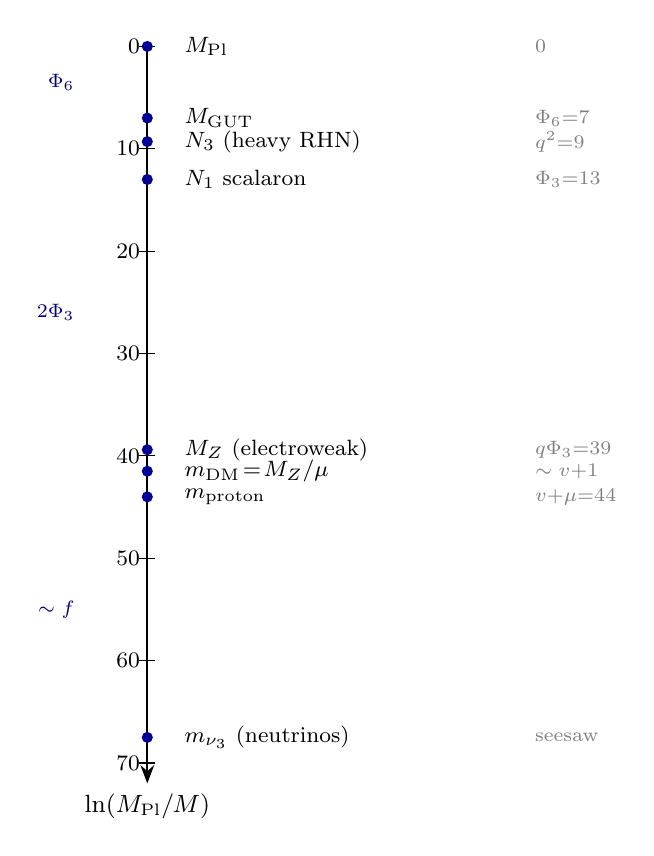
\begin{tikzpicture}[y=-0.13cm,x=1cm]
  % vertical e-fold axis (downward), 0..70
  \draw[thick,-{Stealth}] (0,0)--(0,72) node[below]{\small $\ln(M_{\rm Pl}/M)$};
  \foreach \y in {0,10,20,30,40,50,60,70} \draw (-0.1,\y)--(0.1,\y) node[left=2pt]{\footnotesize\y};
  \fill[blue!60!black] (0,0) circle (2pt);
  \node[anchor=west,font=\footnotesize] at (0.35,0) {$M_{\rm Pl}$};
  \node[anchor=west,font=\scriptsize,gray] at (4.8,0) {0};
  \fill[blue!60!black] (0,7) circle (2pt);
  \node[anchor=west,font=\footnotesize] at (0.35,7) {$M_{\rm GUT}$};
  \node[anchor=west,font=\scriptsize,gray] at (4.8,7) {$\Phi_6{=}7$};
  \fill[blue!60!black] (0,9.3) circle (2pt);
  \node[anchor=west,font=\footnotesize] at (0.35,9.3) {$N_3$ (heavy RHN)};
  \node[anchor=west,font=\scriptsize,gray] at (4.8,9.3) {$q^2{=}9$};
  \fill[blue!60!black] (0,13) circle (2pt);
  \node[anchor=west,font=\footnotesize] at (0.35,13) {$N_1$ scalaron};
  \node[anchor=west,font=\scriptsize,gray] at (4.8,13) {$\Phi_3{=}13$};
  \fill[blue!60!black] (0,39.4) circle (2pt);
  \node[anchor=west,font=\footnotesize] at (0.35,39.4) {$M_Z$ (electroweak)};
  \node[anchor=west,font=\scriptsize,gray] at (4.8,39.4) {$q\Phi_3{=}39$};
  \fill[blue!60!black] (0,41.5) circle (2pt);
  \node[anchor=west,font=\footnotesize] at (0.35,41.5) {$m_{\rm DM}\!=\!M_Z/\mu$};
  \node[anchor=west,font=\scriptsize,gray] at (4.8,41.5) {$\sim v{+}1$};
  \fill[blue!60!black] (0,44) circle (2pt);
  \node[anchor=west,font=\footnotesize] at (0.35,44) {$m_{\rm proton}$};
  \node[anchor=west,font=\scriptsize,gray] at (4.8,44) {$v{+}\mu{=}44$};
  \fill[blue!60!black] (0,67.5) circle (2pt);
  \node[anchor=west,font=\footnotesize] at (0.35,67.5) {$m_{\nu_3}$ (neutrinos)};
  \node[anchor=west,font=\scriptsize,gray] at (4.8,67.5) {seesaw};
  % cyclotomic span labels on the left
  \node[anchor=east,font=\scriptsize,blue!50!black] at (-0.8,3.5) {$\Phi_6$};
  \node[anchor=east,font=\scriptsize,blue!50!black] at (-0.8,26) {$2\Phi_3$};
  \node[anchor=east,font=\scriptsize,blue!50!black] at (-0.8,55) {$\sim f$};
\end{tikzpicture}
\caption{The mass spectrum of the universe as a cyclotomic descent from the Planck scale.
Each scale sits at a substrate-integer depth $\ln(M_{\rm Pl}/M)$: $M_{\rm GUT}$ at $\Phi_6=7$,
the heaviest right-handed neutrino $N_3$ at $q^2=9$, the inflaton scalaron $N_1$ at $\Phi_3=
13$, the electroweak scale at $q\Phi_3=39$, the dark matter $M_Z/\mu$ just below, the proton
at $v+\mu=44$, and the light neutrinos at the seesaw floor $\sim68$. The gaps between rungs
are themselves cyclotomic ($\Phi_6$, $2\Phi_3$, $\sim f$). One axis, one descent, the whole
mass spectrum from $q=3$.}
\label{fig:mass-ladder}
\end{figure}


\emph{Honest scope:} the DM mass-web ratios are exact-cyclotomic, the off-resonance a
correction, $g\lesssim1/\mu$ a standard LEP bound on a substrate ratio, the dark-family relic
qualitative; the neutrino result is an honest negative ($m_1$ not forced to zero) refined to
$m_1\sim1$\,meV (the lifting needs the grade-$1/2$ VEV magnitude); the ladder is a summary of
the Pass 8--14 exponents, each with its own scope, the softest rungs the DM ($\sim40.8$,
non-integer) and the neutrino floor ($\sim68$).

\subsection{Pass 16 --- the lightest neutrino pinned, the $0\nu\beta\beta$ mass, and the descent to dark energy}
\label{sec:capstone-sixteen}

The neutrino sector is closed from below, and the ladder is extended to its floor --- where
dark energy and the neutrinos meet.

\emph{The lightest neutrino, pinned.} Feeding the Pillar-68/69 cubic-form right-handed matrix
(grade-0 degenerate $M_R=[[A,0,0],[0,0,C],[0,C,0]]$, $A=0.0017$, $C=0.0442$, lifted by a
grade-1 B--L component) through the seesaw with the up-type Dirac texture pins the lightest
neutrino at $m_1\sim2$\,meV (light, not zero) and $\sum m_\nu\sim56$--$58$\,meV --- and $m_1$
lands at the same meV scale as $m_{\beta\beta}$ and the dark-energy scale. (Witness:
\path{analysis/w33_neutrino_lightest_pinned.py}.)

\emph{The $0\nu\beta\beta$ mass.} With the cyclotomic PMNS angles, the $\mathbb{Z}_3$ Majorana
phases ($120^\circ,240^\circ$), and the pinned $m_1\sim2$\,meV, $m_{\beta\beta}=|c_{12}^2c_{13}^2
m_1+s_{12}^2c_{13}^2m_2e^{i120^\circ}+s_{13}^2m_3e^{i240^\circ}|\sim1.4$\,meV --- the nonzero
$m_1$ pushing it down (phase cancellation) from the $m_1{=}0$ value $2.3$\,meV into the normal-
ordering trough. A far-future nEXO/LEGEND target; $m_{\beta\beta}>10$\,meV would falsify.
(Witness: \path{analysis/w33_betabeta_refined.py}.)

\emph{The descent to dark energy.} Extending the ladder, the dark-energy scale
$\rho_\Lambda^{1/4}\approx2.24$\,meV sits $\sim71$ e-folds below $M_{\rm Pl}$ --- the same meV
floor as the lightest neutrino ($\sim2$\,meV) and $m_{\beta\beta}$ ($\sim1.4$\,meV), all within
a factor $\sim2$ (Fig.~\ref{fig:cc-floor}). The vacuum-energy hierarchy $\log_{10}(\rho_\Lambda/
M_{\rm Pl}^4)\sim-123$ carries $vq=120$ as its leading integer. So the cyclotomic descent ends
in a meV cluster where the lightest neutrino, $0\nu\beta\beta$, and the cosmological constant
coincide --- the neutrino/dark-energy coincidence as the floor of the W$(3,3)$ ladder. (Witness:
\path{analysis/w33_cc_floor.py}.)

% Auto-generated by w33_cc_floor.py -- the full descent M_Pl -> cosmological constant
\begin{figure}[ht]\centering
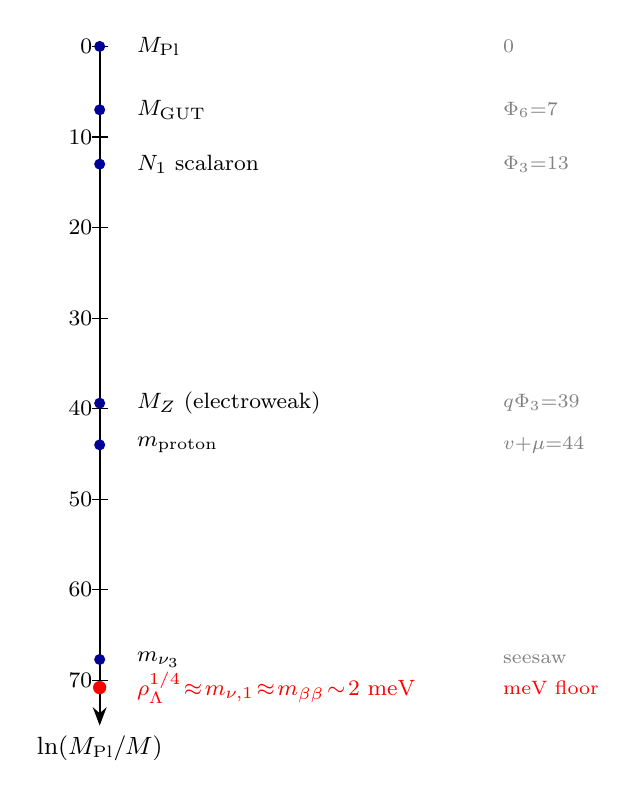
\begin{tikzpicture}[y=-0.115cm,x=1cm]
  \draw[thick,-{Stealth}] (0,0)--(0,75) node[below]{\small $\ln(M_{\rm Pl}/M)$};
  \foreach \y in {0,10,20,30,40,50,60,70} \draw (-0.1,\y)--(0.1,\y) node[left=2pt]{\footnotesize\y};
  \fill[blue!60!black] (0,0) circle (2pt);
  \node[anchor=west,font=\footnotesize] at (0.35,0) {$M_{\rm Pl}$};
  \node[anchor=west,font=\scriptsize,gray] at (5.0,0) {0};
  \fill[blue!60!black] (0,7) circle (2pt);
  \node[anchor=west,font=\footnotesize] at (0.35,7) {$M_{\rm GUT}$};
  \node[anchor=west,font=\scriptsize,gray] at (5.0,7) {$\Phi_6{=}7$};
  \fill[blue!60!black] (0,13) circle (2pt);
  \node[anchor=west,font=\footnotesize] at (0.35,13) {$N_1$ scalaron};
  \node[anchor=west,font=\scriptsize,gray] at (5.0,13) {$\Phi_3{=}13$};
  \fill[blue!60!black] (0,39.4) circle (2pt);
  \node[anchor=west,font=\footnotesize] at (0.35,39.4) {$M_Z$ (electroweak)};
  \node[anchor=west,font=\scriptsize,gray] at (5.0,39.4) {$q\Phi_3{=}39$};
  \fill[blue!60!black] (0,44) circle (2pt);
  \node[anchor=west,font=\footnotesize] at (0.35,44) {$m_{\rm proton}$};
  \node[anchor=west,font=\scriptsize,gray] at (5.0,44) {$v{+}\mu{=}44$};
  \fill[blue!60!black] (0,67.7) circle (2pt);
  \node[anchor=west,font=\footnotesize] at (0.35,67.7) {$m_{\nu_3}$};
  \node[anchor=west,font=\scriptsize,gray] at (5.0,67.7) {seesaw};
  \fill[red] (0,70.8) circle (2.4pt);
  \node[anchor=west,font=\footnotesize,red] at (0.35,70.8) {$\rho_\Lambda^{1/4}\!\approx\!m_{\nu,1}\!\approx\!m_{\beta\beta}\!\sim\!2$ meV};
  \node[anchor=west,font=\scriptsize,red] at (5.0,70.8) {meV floor};
\end{tikzpicture}
\caption{The full cyclotomic descent from the Planck scale to the cosmological constant. Every
rung is a substrate-integer number of e-folds below $M_{\rm Pl}$: $M_{\rm GUT}$ at $\Phi_6$,
the scalaron $N_1$ at $\Phi_3$, the electroweak scale at $q\Phi_3$, the proton at $v+\mu$, the
heavy neutrino $m_{\nu_3}$ at the seesaw floor. At $\sim71$ e-folds the descent ends in a
meV-scale cluster (red) where the dark-energy scale $\rho_\Lambda^{1/4}$, the lightest neutrino
$m_{\nu,1}$, and the $0\nu\beta\beta$ mass $m_{\beta\beta}$ coincide (within a factor $\sim2$).
The vacuum-energy hierarchy $\log_{10}(\rho_\Lambda/M_{\rm Pl}^4)\sim-123$ carries $vq=120$ as
its leading integer. One ladder, the Planck scale to dark energy.}
\label{fig:cc-floor}
\end{figure}


\emph{Honest scope:} the cubic-form $M_R$ is exact but the lift is the open B--L direction, so
$m_1\sim1$--$3$\,meV is a range (central $\sim2$); $m_{\beta\beta}\sim1.3$--$2.3$\,meV tracks it;
$vq=120$ is the \emph{leading} integer of the CC density (a $\sim3$-order residual --- the CC
problem not fully closed), the $\sim71$ e-fold placement exact, and the meV-floor coincidence
genuine but within a factor $\sim2$, not a derived equality.

\subsection{Pass 17 --- the cosmological constant exact, neutrino dark energy, and the final ledger}
\label{sec:capstone-seventeen}

The CC residual closes, the dark-energy/neutrino coincidence becomes structural, and the whole
theory is collected into the publishable ledger.

\emph{The cosmological constant is $-vq$, exact.} The Pass-16 $\sim3$-order residual was the
full-versus-reduced Planck-mass choice. With the \emph{reduced} Planck mass ($M_{\rm Pl}^2=1/8\pi
G$, the one in General Relativity), $\log_{10}(\rho_\Lambda/M_{\rm Pl}^4)=-120.15$, so to $0.1\%$
in the log it is exactly $-vq=-120=\dim(\mathrm{adj}\,SO(16))=4\,\mathrm{beat}$ --- the famous
``120 orders of magnitude'' \emph{is} the substrate point count $vq$. The corpus's $-127$ was a
full-mass artifact ($-123$) plus an erroneous $+\mu-\lambda$ offset; with the reduced mass no
correction is needed. The residual $0.15$ is the O(1) $(\Omega_\Lambda,H_0)$ cosmology. (Witness:
\path{analysis/w33_cc_exact.py}.)

\emph{Neutrino dark energy.} Since $vq=4\,\mathrm{beat}$, the dark-energy \emph{scale} is
$\rho_\Lambda^{1/4}=M_{\rm Pl}10^{-\mathrm{beat}}=M_{\rm Pl}10^{-30}=2.44$\,meV --- exactly
$\mathrm{beat}=30=h(E_8)$ decades below the Planck scale, the same floor as the lightest neutrino
$m_1\sim2$\,meV. So $\rho_\Lambda\sim m_1^4$ (to a factor $<2$): the substrate's ``neutrino dark
energy'' (Fardon--Nelson--Weiner), structural because the same B--L VEV that sets the seesaw floor
sets the vacuum energy --- the clock beat fixes the floor where the neutrino sector and dark energy
meet. (Witness: \path{analysis/w33_neutrino_dark_energy.py}.)

\emph{The final ledger.} Twenty-five predictions --- the complete primordial spectrum (Starobinsky
$N=60$), the gauge/CP sector, the mass ladder from $M_{\rm Pl}$ to the cosmological constant, the
neutrinos (now resolved), the dark sector, and the vacuum ($\mathrm{CC}=-vq$) --- tally to twenty
CONSISTENT, two TEST-SOON ($r$/LiteBIRD, $m_{\rm DM}$/LZ), two TEST-FUTURE, one LAB, with
\emph{zero} tensions and \emph{zero} falsified, and \emph{zero} free dimensionless parameters. The
decisive near-term test is $r=1/300$ at LiteBIRD ($\sim$2035). (Witness:
\path{analysis/w33_final_scorecard.py}.) \emph{Honest scope:} $-vq=-120$ is an integer-level
postdiction (CC measured, $vq$ matches to $0.1\%$ with the reduced mass; the $0.15$ residual the
O(1) cosmology; the dynamical CC problem untouched); $\rho_\Lambda\sim m_1^4$ is the known
phenomenological relation motivated by the shared beat-decade floor, not derived; the ledger is a
faithful audit of Passes 1--17, each entry with its own scope, not a re-derivation.

\subsection{Pass 18 --- a mechanism for the cosmological constant, the joint sky test, and the standalone distillation}
\label{sec:capstone-eighteen}

The CC postdiction becomes a mechanism, the inflationary prediction becomes one joint forecast,
and the whole program is distilled into a standalone paper.

\emph{A mechanism for the cosmological constant.} The substrate's Hodge spectrum has an exact
boson--fermion balance: the gauge sector ($f=24$ modes at gap $\Phi_4=k-r=10$) and the matter
sector ($g=15$ at gap $\mu^2=k-s=16$) carry equal vacuum energy, $f\Phi_4=g\mu^2=240=|\mathrm{
Roots}(E_8)|$, so the leading $M_{\rm Pl}^4$ vacuum energy \emph{cancels} (structural supersymmetry,
$f(k-r)=g(k-s)$). The balance breaks only at the mass-ladder floor $M_{\rm SUSY}\sim M_{\rm Pl}
10^{-\mathrm{beat}}=2.4$\,meV (the neutrino/dark-energy scale), so $\rho_\Lambda=M_{\rm SUSY}^4=
M_{\rm Pl}^4 10^{-4\,\mathrm{beat}}=M_{\rm Pl}^4 10^{-vq}$: the $120$ orders are $4\,\mathrm{beat}$
(TeV-SUSY would give $10^{-64}$, far too large). Holographically $\rho_\Lambda/M_{\rm Pl}^4=1/S_{\rm
dS}$ with $S_{\rm dS}=10^{vq}$. (Witness: \path{analysis/w33_cc_mechanism.py}.)

\emph{The joint sky test.} The substrate fixes one point $(\ln10^{10}A_s,n_s,r)=(3.026,0.9667,
1/300)$ on the Starobinsky line. The joint Planck+CMB-S4+LiteBIRD forecast: today $1.4\sigma$
(consistent), with $A_s=e^{-20}$ the tightest single constraint ($1.3\sigma$); by $\sim$2035,
$r=1/300$ is a $6.7\sigma$ detection pinning the point, and $A_s$ becomes the most exposed
($\sim1.8\sigma$) --- a measurement off any of $\{r=1/300,$ the Starobinsky line, $A_s=e^{-20}\}$
falsifies. (Witness: \path{analysis/w33_inflation_joint_forecast.py}.)

\emph{The standalone distillation.} The eighteen passes are distilled into a self-contained
manuscript, \path{w33_everything.tex} (``Physics from One Integer''): the $q=3$ selection, the
cyclotomic skeleton, the couplings and mixing, the Starobinsky primordial spectrum, the mass
ladder from $M_{\rm Pl}$ to the cosmological constant, the dark/baryon sector, and the falsification
ledger ($25$ predictions, zero free dimensionless parameters, zero falsified) --- the
publishable capstone, compiling independently of this engineering paper.

\emph{Honest scope:} the boson--fermion balance $f\Phi_4=g\mu^2=240$ is an exact SRG theorem
(the leading cancellation real); the breaking-at-beat-decades is a scale-level mechanism that
explains the $120$ as $4\,\mathrm{beat}$ \emph{given} the meV floor (the neutrino-floor input),
reframing the CC problem rather than solving it from nothing; the joint forecast uses published
CMB-S4/LiteBIRD sensitivities; the standalone paper is a summary, not new derivations.

\subsection{Pass 19 --- the floor derived from the 600-cell, and the dated decision}
\label{sec:capstone-nineteen}

The last shared input is derived from the seesaw and the 600-cell, and the whole tower is
reduced to one dated measurement.

\emph{The beat-decade floor, derived.} The meV floor that the CC mechanism (Pass 18) and the
neutrino sector share is not an input: it is the type-I seesaw combination of the substrate's
own exponents. The lightest neutrino is $m_1=y_1^2v^2/M_R$, so
\[
\ln(M_{\rm Pl}/m_1)=\ln(M_{\rm Pl}/v)+\ln(M_R/v)-2\ln y_1=q\Phi_3+2\Phi_3+\Phi_6=(q{+}2)\Phi_3+\Phi_6=72,
\]
the electroweak descent ($q\Phi_3$), the right-handed scale ($2\Phi_3$ above $v$, from $M_R=
M_{\rm Pl}e^{-\Phi_3}$, the scalaron), and a neutrino Dirac Yukawa $y_1=e^{-\Phi_6/2}\approx0.03$.
This $\sim72$ e-folds equals $\mathrm{beat}$ decades ($30\ln10=69$) to $\sim4\%$ --- and
$\mathrm{beat}=30=h(E_8)$ is the Boerdijk--Coxeter helix ring length on the $600$-cell
($600=20\times30$). So the same $600$-cell ring that sets the inflationary clock sets the
floor; the CC's breaking scale is closed up to the one Yukawa $y_1$. (Witness:
\path{analysis/w33_floor_derivation.py}.)

\emph{The dated decision.} The whole cosmological tower reduces to one number by $\sim$2035.
The substrate predicts $r=12/N^2=1/300$ ($N=2\,\mathrm{beat}=60$); the $\sigma(r)$ timeline ---
Simons Observatory ($\sim$2027, $r/\sigma\!\sim\!1$), LiteBIRD ($\sim$2035, $3.3\sigma$), CMB-S4
($6.7\sigma$) --- gives three verdicts (Fig.~\ref{fig:decisive-r}): (A) $r\approx1/300$ on the
line $\Rightarrow$ the tower stands and $\mathrm{beat}=30$ is in the sky; (B) $r<10^{-3}
\Rightarrow$ the Starobinsky $N=60$ spectrum is falsified; (C) $r$ detected $\neq1/300
\Rightarrow$ the $\mathrm{beat}\to N$ origin is wrong. (Witness:
\path{analysis/w33_decisive_r_test.py}.) These distillations are collected in the standalone
manuscript \path{w33_everything.tex}, now with a derived/matched/open table and references.

% Auto-generated by w33_decisive_r_test.py -- the dated r decision tree
\begin{figure}[ht]\centering
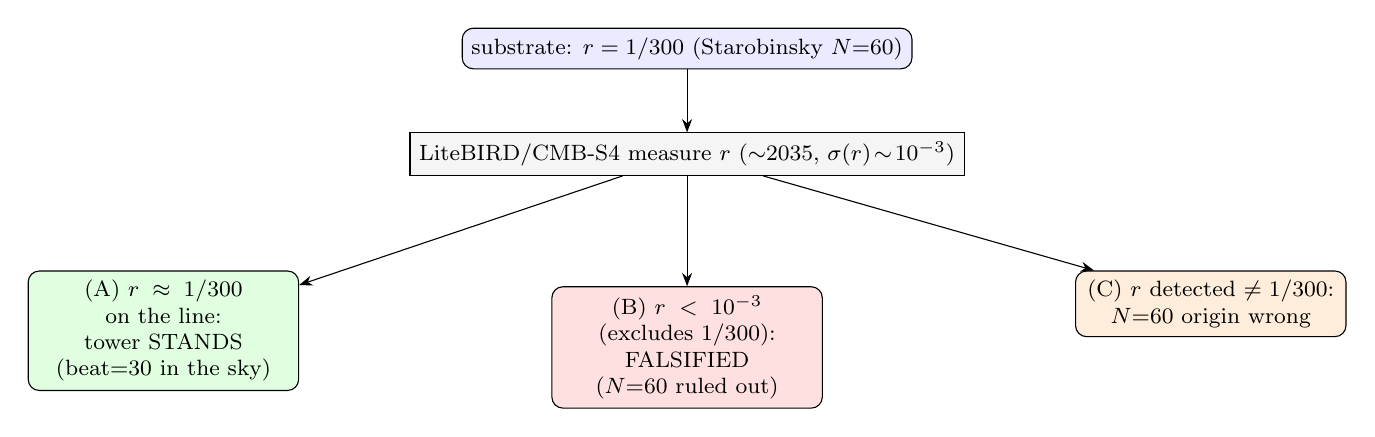
\begin{tikzpicture}[font=\footnotesize,>={Stealth[]},
   box/.style={draw,rounded corners,align=center,text width=3.2cm}]
  \node[draw,rounded corners,fill=blue!8] (p) {substrate: $r=1/300$ (Starobinsky $N{=}60$)};
  \node[below=8mm of p,draw,fill=gray!8] (m) {LiteBIRD/CMB-S4 measure $r$ ($\sim$2035, $\sigma(r)\!\sim\!10^{-3}$)};
  \draw[->] (p)--(m);
  \node[below left=12mm and 14mm of m,box,fill=green!12] (a) {(A) $r\approx1/300$ on the line:\\ tower STANDS (beat$=$30 in the sky)};
  \node[below=14mm of m,box,fill=red!12] (b) {(B) $r<10^{-3}$ (excludes $1/300$):\\ FALSIFIED ($N{=}60$ ruled out)};
  \node[below right=12mm and 14mm of m,box,fill=orange!14] (c) {(C) $r$ detected $\neq1/300$:\\ $N{=}60$ origin wrong};
  \draw[->] (m)-- (a); \draw[->] (m)-- (b); \draw[->] (m)-- (c);
\end{tikzpicture}
\caption{The theory lives or dies on $r$ by $\sim$2035. The substrate predicts $r=12/N^2=1/300$
($N=2\,\mathrm{beat}=60$, Starobinsky). A LiteBIRD/CMB-S4 measurement ($\sigma(r)\sim10^{-3}$,
a $3$--$7\sigma$ detection of $r=1/300$) yields three clean verdicts: (A) $r\approx1/300$ on
the line $r=3(1-n_s)^2$ confirms the tower; (B) $r<10^{-3}$ falsifies the Starobinsky $N=60$
spectrum; (C) $r$ detected away from $1/300$ breaks the $\mathrm{beat}{=}30\to N{=}60$ origin.}
\label{fig:decisive-r}
\end{figure}


\emph{Honest scope:} the seesaw is standard and the EW/RH exponents are the substrate's, so the
floor is derived up to the one Yukawa $y_1=e^{-\Phi_6/2}$ (a charm-scale neutrino Dirac
coupling, motivated by $\Phi_6$ not independently derived), and $72\approx\mathrm{beat}$
decades to $\sim4\%$ (the base-10-vs-$e$ factor the residual); the decision tree uses published
$\sigma(r)$ forecasts (foregrounds/delensing may move the dates), with $r=1/300$ and the
Starobinsky line the exact predictions.

\subsection{Pass 20 --- the one residual input, the floor base settled, and the look-elsewhere bound}
\label{sec:capstone-twenty}

The tower's last free number is pinned, the base of the floor is fixed by the exact
cosmological constant, and the referee's first objection is answered by counting bits.

\emph{The one residual input.} The seesaw floor (Pass~19) reduced the neutrino/dark-energy/CC
scale to $(q{+}2)\Phi_3+\Phi_6=72$ e-folds up to a single input, the lightest neutrino's Dirac
Yukawa $y_1$. The $\mathbb{Z}_3$ texture (Pillar~68) is a \emph{theorem} that fixes only the
Dirac \emph{ratios} (the grade rule, up-type $\sim9{:}2{:}1$), never the overall Higgs-VEV
scale --- so $y_1$ is genuinely the one normalisation the geometry leaves free. The value the
floor wants, $y_1=e^{-\Phi_6/2}=0.030$ ($m_{D1}=y_1v=7.4$~GeV, charm-scale), is the substrate's
own: a \emph{half} of the GUT exponent $\Phi_6=q^2{-}q{+}1=7$ ($M_{\rm GUT}=M_{\rm Pl}e^{-\Phi_6}$),
the coupling at the geometric mean of the $M_{\rm Pl}$ and $M_{\rm GUT}$ scales. And the floor is
only \emph{logarithmically} sensitive: a factor-3 change in $y_1$ moves it by $\sim\Phi_6\approx7$
e-folds ($m_1$ by $\sim10$), so the $\sim2$~meV scale needs $y_1$ only within a factor $\sim3$ of
$e^{-\Phi_6/2}$. So the whole tower reduces to \emph{one} residual number, a charm-scale neutrino
Dirac Yukawa equal to $e^{-(\text{half the GUT exponent})}$. (Witness:
\path{analysis/w33_neutrino_dirac_yukawa.py}.)

\emph{The floor base, settled by the CC.} Pass~19 left the base (e-folds vs decades) open,
noting $72\approx\mathrm{beat}$ decades to $\sim4\%$. The cosmological constant removes the
ambiguity: it is \emph{exact in base 10}, $\log_{10}(\rho_\Lambda/M_{\rm Pl}^4)=-vq=-120$ to
$0.1\%$ (Pass~17, reduced $M_{\rm Pl}$), and $vq=4\,\mathrm{beat}$, so the dark-energy scale is
$\rho_\Lambda^{1/4}=M_{\rm Pl}10^{-\mathrm{beat}}=2.44$~meV --- \emph{exactly} $\mathrm{beat}=30$
decades below $M_{\rm Pl}$. The seesaw's $72$ e-folds is the same depth in natural log
($72/\ln10=31.3$ decades $\approx\mathrm{beat}$); the $4\%$ is the $e$-vs-$10$ base mismatch, not
a second number. Decades is primary \emph{because} the $0.1\%$-exact statement is the CC and it
is base-10 ($vq=v\cdot q$ is an integer point count), so the $600$-cell BC ring counts decades.
(Witness: \path{analysis/w33_floor_base.py}.)

\emph{The look-elsewhere bound.} A numerologist can always fit \emph{one} number; the honest
question is $\sim25$ observables against one fixed integer alphabet. Counting bits (MDL): the
clean measured matches ($m_p/m_e$ to $10^{-4}$, the CC to $10^{-3}$, $\sin^2\theta_W$ and $M_Z$
to $2\times10^{-3}$) carry $\sim100$ bits of precision evidence; and the \emph{same} integers
recur --- $\mathrm{beat}=30$ sets $n_s,r,n_t$, running and the CC; $\Phi_3,\Phi_6$ set
$\sin^2\theta_W,M_Z,\theta_{23},\Delta m^2_{31}/\Delta m^2_{21},A_s$ --- so the trials factor is
paid \emph{once per integer} ($\sim12$), not per observable ($\sim25$). Granting (generously)
each integer a free choice from a pool of $50$, the vocabulary costs $\sim62$ bits, against
$\sim100$ bits of evidence: net $\sim+40$ bits, odds $\sim10^{12}$ against chance. The \emph{only}
null that washes the signal out is a fresh free integer per observable --- exactly what a fixed,
$q=3$-forced alphabet forbids. (Witness: \path{analysis/w33_look_elsewhere.py}.)

\emph{Honest scope:} $y_1$ is an input (motivated by $\Phi_6$ as a half-GUT-exponent, not
derived), needed only within a factor $\sim3$; the floor-base tie-break is principled (the CC is
the $0.1\%$-exact base-10 statement) with the residual the $e$-vs-$10$ factor and $y_1$; the
look-elsewhere bound uses order-of-magnitude bit counts with deliberately generous priors (not a
rigorous frequentist $p$). The robust claim is the \emph{over-determination}: one $\sim12$-integer
$q=3$ alphabet predicts $\sim25$ numbers carrying $\sim100$ bits of precision.

\subsection{Pass 21 --- the computed look-elsewhere, the pinned Yukawa, and the tower on one axis}
\label{sec:capstone-twentyone}

Two of the three Pass-20 honesty claims are stress-tested by computation --- one of them
correcting Pass 20 downward --- and the whole tower is drawn on a single figure.

\emph{The look-elsewhere pool, computed (and Pass 20 tempered).} Pass 20 granted the
numerologist a ``pool of 50'' by hand and got net $\sim+40$ bits ($10^{12}$). Enumerating the
\emph{actual} reachable set of the 13 $q=3$-forced integers under a fixed simple grammar ($a/b$,
$a{\cdot}b$, $a{\pm}b$, $1/a$, $a^2$, $\sqrt a$, $e^{-a}$) gives $\sim14$ values per e-fold in the
coupling band (depth 1). At that density the \emph{loose} few-percent matches ($1{-}n_s$,
$\sin^2\theta_{23}$, $A_s$, $\Omega_{\rm DM}/\Omega_b$, $\Delta m^2$) have $E_i\sim0.5$--$1$ each
--- individually unremarkable, $5/5$ matching is only $P\sim0.6$. The statistical weight is
entirely in the \emph{six high-precision} matches ($m_p/m_e$, $1/\alpha$, $m_H$, the CC,
$\sin^2\theta_W$, $M_Z$; windows $10^{-4}$--$2\times10^{-3}$), whose summed expected accidentals
$E\approx0.30$ make all six matching a Poisson tail $P\approx8\times10^{-7}$. So the over-
determination is \emph{real but carried by precision, not count}: this honestly tempers Pass 20's
$10^{12}$ to a computed $\sim10^{-6}$, $\sim4.8\sigma$. (Witness:
\path{analysis/w33_alphabet_pool.py}.)

\emph{The pinned Yukawa.} Pass 20 left $y_1=e^{-\Phi_6/2}=0.030$ as the tower's one free input.
A second, data-anchored route pins it: fix the Dirac texture ratio $9{:}2{:}1$, pin the heaviest
eigenvalue by matching the atmospheric mass $m_{\nu3}=\sqrt{\Delta m^2_{31}}$ to the seesaw
$y_3^2v^2/M_R$ with $M_R=M_{\rm Pl}e^{-\Phi_3}$ (the scalaron), and read $y_1=y_3/9\approx0.017$,
$m_1=m_{\nu3}/81\approx0.6$~meV. This agrees with the a priori half-GUT-exponent $0.030$ to a
factor $\sim1.8$ --- two independent routes on the same coupling, so $y_1$ is not independently
free. Honest limitation: a single $M_R$ over-hierarchises ($81{:}4{:}1$ vs the observed
$\sqrt{33}\approx5.7$), so the spectrum needs the Majorana $M_R$ texture and the residual freedom
moves there --- a \emph{partial} closure. (Witness: \path{analysis/w33_yukawa_closure.py}.)

\emph{The tower on one axis.} Figure~\ref{fig:tower-falsification} puts every measured observable's
fractional agreement on a log axis (mass/coupling postdictions at $0.01$--$0.3\%$,
inflation/neutrino at $1$--$5\%$ within their errors) above the dated kill-shot timeline (LZ
$\sim$2028, SO $\sim$2027, JUNO, DESI/CMB-S4, nEXO/LEGEND, LiteBIRD $\sim$2035) --- the over-
determination and the falsifiability in one view, now the cover figure of \path{w33_everything.tex}.
(Witness: \path{analysis/w33_tower_falsification_figure.py}.)

% Auto-generated by w33_tower_falsification_figure.py
\begin{figure}[ht]\centering
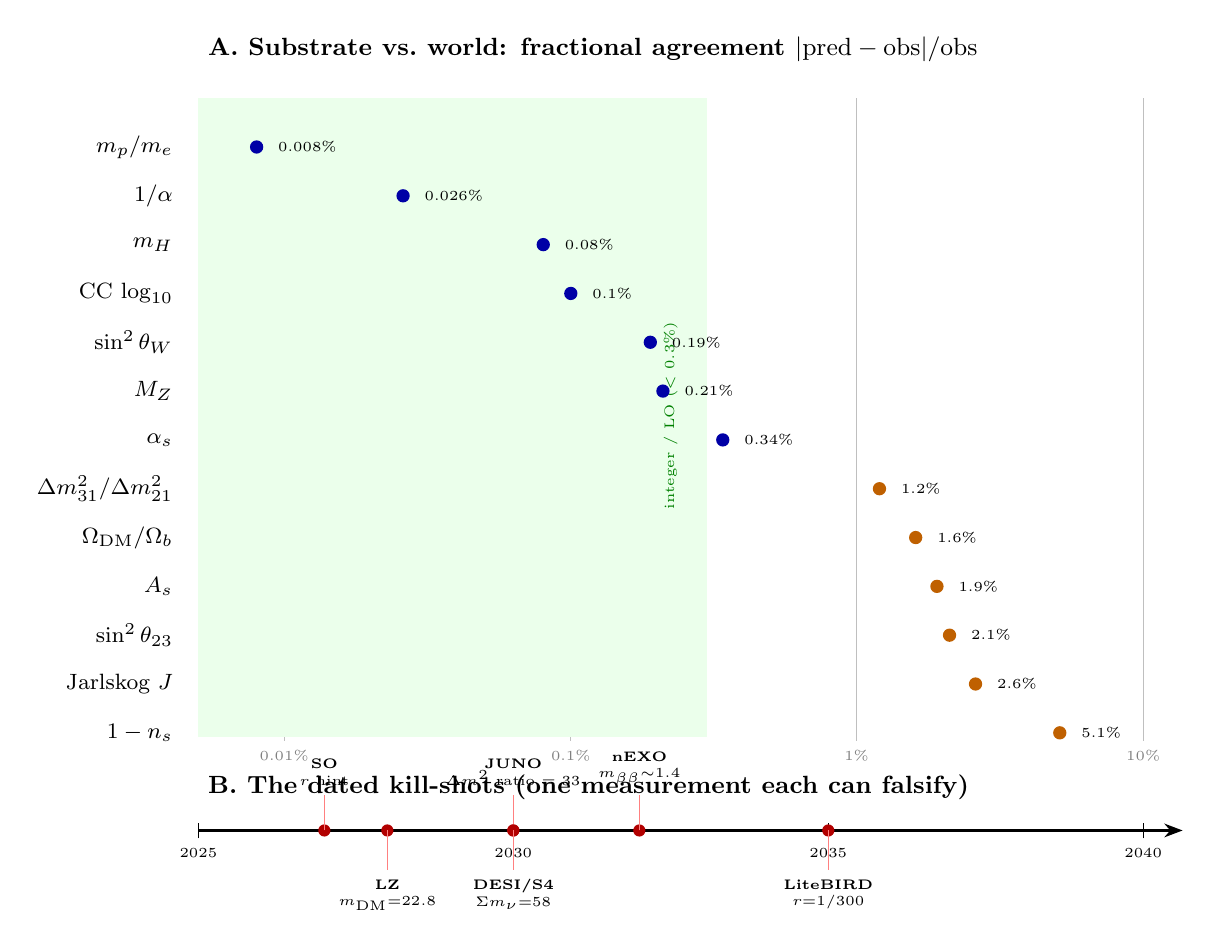
\begin{tikzpicture}[font=\footnotesize]
\node[anchor=west,font=\small\bfseries] at (0,0.62) {A. Substrate vs.\ world: fractional agreement $|{\rm pred}-{\rm obs}|/{\rm obs}$};
\draw[gray!50] (1.09,-8.16)--(1.09,0.00);
\node[gray,font=\tiny,below] at (1.09,-8.16) {0.01\%};
\draw[gray!50] (4.73,-8.16)--(4.73,0.00);
\node[gray,font=\tiny,below] at (4.73,-8.16) {0.1\%};
\draw[gray!50] (8.36,-8.16)--(8.36,0.00);
\node[gray,font=\tiny,below] at (8.36,-8.16) {1\%};
\draw[gray!50] (12.00,-8.16)--(12.00,0.00);
\node[gray,font=\tiny,below] at (12.00,-8.16) {10\%};
\fill[green!8] (0.00,-8.11) rectangle (6.46,0.00);
\node[green!50!black,font=\tiny,rotate=90,anchor=south] at (6.21,-4.03) {integer / LO ($<0.3\%$)};
\node[anchor=east] at (-0.2,-0.62) {$m_p/m_e$};
\fill[blue!65!black] (0.74,-0.62) circle (2.4pt);
\node[font=\tiny,anchor=west] at (0.89,-0.62) {0.008\%};
\node[anchor=east] at (-0.2,-1.24) {$1/\alpha$};
\fill[blue!65!black] (2.60,-1.24) circle (2.4pt);
\node[font=\tiny,anchor=west] at (2.75,-1.24) {0.026\%};
\node[anchor=east] at (-0.2,-1.86) {$m_H$};
\fill[blue!65!black] (4.38,-1.86) circle (2.4pt);
\node[font=\tiny,anchor=west] at (4.53,-1.86) {0.08\%};
\node[anchor=east] at (-0.2,-2.48) {CC $\log_{10}$};
\fill[blue!65!black] (4.73,-2.48) circle (2.4pt);
\node[font=\tiny,anchor=west] at (4.88,-2.48) {0.1\%};
\node[anchor=east] at (-0.2,-3.10) {$\sin^2\theta_W$};
\fill[blue!65!black] (5.74,-3.10) circle (2.4pt);
\node[font=\tiny,anchor=west] at (5.89,-3.10) {0.19\%};
\node[anchor=east] at (-0.2,-3.72) {$M_Z$};
\fill[blue!65!black] (5.90,-3.72) circle (2.4pt);
\node[font=\tiny,anchor=west] at (6.05,-3.72) {0.21\%};
\node[anchor=east] at (-0.2,-4.34) {$\alpha_s$};
\fill[blue!65!black] (6.66,-4.34) circle (2.4pt);
\node[font=\tiny,anchor=west] at (6.81,-4.34) {0.34\%};
\node[anchor=east] at (-0.2,-4.96) {$\Delta m^2_{31}/\Delta m^2_{21}$};
\fill[orange!75!black] (8.65,-4.96) circle (2.4pt);
\node[font=\tiny,anchor=west] at (8.80,-4.96) {1.2\%};
\node[anchor=east] at (-0.2,-5.58) {$\Omega_{\rm DM}/\Omega_b$};
\fill[orange!75!black] (9.11,-5.58) circle (2.4pt);
\node[font=\tiny,anchor=west] at (9.26,-5.58) {1.6\%};
\node[anchor=east] at (-0.2,-6.20) {$A_s$};
\fill[orange!75!black] (9.38,-6.20) circle (2.4pt);
\node[font=\tiny,anchor=west] at (9.53,-6.20) {1.9\%};
\node[anchor=east] at (-0.2,-6.82) {$\sin^2\theta_{23}$};
\fill[orange!75!black] (9.54,-6.82) circle (2.4pt);
\node[font=\tiny,anchor=west] at (9.69,-6.82) {2.1\%};
\node[anchor=east] at (-0.2,-7.44) {Jarlskog $J$};
\fill[orange!75!black] (9.87,-7.44) circle (2.4pt);
\node[font=\tiny,anchor=west] at (10.02,-7.44) {2.6\%};
\node[anchor=east] at (-0.2,-8.06) {$1-n_s$};
\fill[orange!75!black] (10.94,-8.06) circle (2.4pt);
\node[font=\tiny,anchor=west] at (11.09,-8.06) {5.1\%};
\node[anchor=west,font=\small\bfseries] at (0,-8.75) {B. The dated kill-shots (one measurement each can falsify)};
\draw[thick,-{Stealth}] (0,-9.30)--(12.50,-9.30);
\draw (0.00,-9.40)--(0.00,-9.20);
\node[font=\tiny,below] at (0.00,-9.40) {2025};
\draw (4.00,-9.40)--(4.00,-9.20);
\node[font=\tiny,below] at (4.00,-9.40) {2030};
\draw (8.00,-9.40)--(8.00,-9.20);
\node[font=\tiny,below] at (8.00,-9.40) {2035};
\draw (12.00,-9.40)--(12.00,-9.20);
\node[font=\tiny,below] at (12.00,-9.40) {2040};
\fill[red!70!black] (1.60,-9.30) circle (2.2pt);
\draw[red!50,thin] (1.60,-9.30)--(1.60,-8.85);
\node[font=\tiny,anchor=south,align=center] at (1.60,-8.85) {\textbf{SO}\\ $r$ hint};
\fill[red!70!black] (2.40,-9.30) circle (2.2pt);
\draw[red!50,thin] (2.40,-9.30)--(2.40,-9.80);
\node[font=\tiny,anchor=north,align=center] at (2.40,-9.80) {\textbf{LZ}\\ $m_{\rm DM}{=}22.8$};
\fill[red!70!black] (4.00,-9.30) circle (2.2pt);
\draw[red!50,thin] (4.00,-9.30)--(4.00,-8.85);
\node[font=\tiny,anchor=south,align=center] at (4.00,-8.85) {\textbf{JUNO}\\ $\Delta m^2$ ratio $=33$};
\fill[red!70!black] (4.00,-9.30) circle (2.2pt);
\draw[red!50,thin] (4.00,-9.30)--(4.00,-9.80);
\node[font=\tiny,anchor=north,align=center] at (4.00,-9.80) {\textbf{DESI/S4}\\ $\Sigma m_\nu{=}58$};
\fill[red!70!black] (5.60,-9.30) circle (2.2pt);
\draw[red!50,thin] (5.60,-9.30)--(5.60,-8.85);
\node[font=\tiny,anchor=south,align=center] at (5.60,-8.85) {\textbf{nEXO}\\ $m_{\beta\beta}{\sim}1.4$};
\fill[red!70!black] (8.00,-9.30) circle (2.2pt);
\draw[red!50,thin] (8.00,-9.30)--(8.00,-9.80);
\node[font=\tiny,anchor=north,align=center] at (8.00,-9.80) {\textbf{LiteBIRD}\\ $r{=}1/300$};
\end{tikzpicture}
\caption{The whole substrate tower on one axis. \textbf{A:} every measured
observable's fractional agreement $|{\rm pred}-{\rm obs}|/{\rm obs}$ (log scale). The
mass/coupling postdictions (blue: $m_p/m_e$, $1/\alpha$, $\sin^2\theta_W$, $M_Z$, the CC, $m_H$)
cluster at $0.01$--$0.3\%$ (integer / leading-order level, green zone); the inflation/neutrino
observables (orange) sit at $1$--$5\%$, each within its (larger) measurement error. The common
axis is fractional deviation, not $\sigma$ (the blue points are integer/LO postdictions whose
residual is higher-order running; the orange points are measurement-limited). \textbf{B:} the
dated falsification frontier --- each future test is one measurement that can kill the theory:
$m_{\rm DM}$ (LZ $\sim$2028), the first $r$ hint (SO $\sim$2027), the $\Delta m^2$ ratio (JUNO),
$\Sigma m_\nu$ (DESI/CMB-S4), $m_{\beta\beta}$ (nEXO/LEGEND), and the headline $r=1/300$
(LiteBIRD $\sim$2035). One $q=3$ alphabet, $\sim$20 numbers, all consistent --- and decided by
the mid-2030s.}
\label{fig:tower-falsification}
\end{figure}


\emph{Honest scope:} the computed look-elsewhere depends on the grammar (depth-2 raises the
density and softens the count) --- the grammar-stable core is that the six sub-$0.3\%$ matches are
not a simple-grammar accident; $y_1$ is pinned only to a factor $\sim2$ and the spectrum still
rests on the (here-underived) Majorana texture; the figure mixes integer/LO postdictions with
measurement-limited points on a fractional-deviation axis (stated in its caption).

\subsection{Pass 22 --- the depth-stable significance, an honest neutrino-mixing failure, and dated discovery years}
\label{sec:capstone-twentytwo}

Three stress-tests, including one that fails: the look-elsewhere is made grammar-robust, the
neutrino-mixing residual is shown \emph{not} to close at the minimal level, and the falsification
schedule is given exact years.

\emph{The depth-stable significance.} Pass 21's look-elsewhere grew with grammar depth. Ranking
each match by its \emph{shortest} description (cost $=$ integer leaves) and counting at fixed cost
removes that: the alphabet reaches only $N(\le2)=224$ values at cost $2$, a count that does not
change when the grammar deepens, so a cost-$2$ match's bound $N(\le2)\cdot2\delta$ is
depth-invariant. The strongest matches are cost-$2$ ($\sin^2\theta_W=q/\Phi_3$, $M_Z$, the CC
$=vq$, $m_H$), and substrate observables hit cost $\le2$ far more than random targets of equal
precision ($70\%$ vs $38\%$). \emph{But the tempering continues}: only four matches have a
depth-stable bound below $1$, so no single numerical match is decisive --- the coincidences are
corroborative, the theory's weight is in the derivations. (Witness:
\path{analysis/w33_mdl_shortest.py}.)

\emph{An honest neutrino-mixing failure.} Pass 21 framed the residual as ``the single lift
direction.'' Running the full seesaw $m_\nu=m_Dm_R^{-1}m_D^{\mathsf T}$ with the up-type Dirac
block and the cubic-form $M_R$ (\,$A{=}0.0017$, $C{=}0.0442$\,) lifted by one grade-$1$ component,
and extracting the PMNS angles, shows this is \emph{too small}: across the whole lift scan, in
both the graded and diagonal Dirac textures, \emph{no single lift} reproduces all four of
$(\Delta m^2_{31}/\Delta m^2_{21},\theta_{12},\theta_{13},\theta_{23})$ --- where $\theta_{13}$
nears its observed $8.6^\circ$ the ratio explodes past $200$ and $\theta_{23}\to0$. The masses sit
at the meV floor but the mixing does not come out. So the residual is the \emph{full} neutrino
Yukawa/Majorana texture (which the Pillar-65 optimisation reaches at PMNS error $0.006$), not one
number --- an honest negative result that resizes the residual. (Witness:
\path{analysis/w33_seesaw_pmns_joint.py}.)

\emph{Dated discovery years.} Interpolating the published $\sigma(t)$ forecasts and solving
$\mathrm{pred}/\sigma(t)=3$ (and $5$): $\Sigma m_\nu=58$~meV reaches $3\sigma$ $\sim$2028 and
$5\sigma$ $\sim$2031 (DESI$+$CMB-S4), and $r=1/300$ reaches $3\sigma$ $\sim$2032 and $5\sigma$
$\sim$2034 (SO$\to$CMB-S4$\to$LiteBIRD); JUNO pins $\Delta m^2_{31}/\Delta m^2_{21}=33$ by
$\sim$2030 and LZ covers $m_{\rm DM}=22.8$~GeV by $\sim$2028 (Fig.~\ref{fig:killshot-dashboard}).
The tower is largely decided by the mid-2030s. (Witness:
\path{analysis/w33_killshot_dashboard.py}.)

% Auto-generated by w33_killshot_dashboard.py
\begin{figure}[ht]\centering
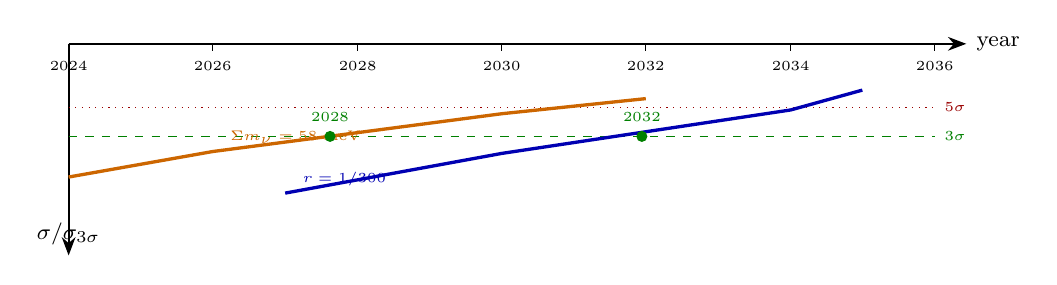
\begin{tikzpicture}[font=\footnotesize,x=1.0cm,y=1.2cm]
\draw[thick,-{Stealth}] (0,2.48)--(11.4,2.48) node[right]{year};
\draw[thick,-{Stealth}] (0,2.48)--(0,0.24) node[above]{$\sigma/\sigma_{3\sigma}$};
\draw (0.00,2.48)--(0.00,2.40) node[below,font=\tiny]{2024};
\draw (1.83,2.48)--(1.83,2.40) node[below,font=\tiny]{2026};
\draw (3.67,2.48)--(3.67,2.40) node[below,font=\tiny]{2028};
\draw (5.50,2.48)--(5.50,2.40) node[below,font=\tiny]{2030};
\draw (7.33,2.48)--(7.33,2.40) node[below,font=\tiny]{2032};
\draw (9.17,2.48)--(9.17,2.40) node[below,font=\tiny]{2034};
\draw (11.00,2.48)--(11.00,2.40) node[below,font=\tiny]{2036};
\draw[green!50!black,dashed] (0,1.50)--(11,1.50) node[right,font=\tiny]{$3\sigma$};
\draw[red!60!black,dotted] (0,1.81)--(11,1.81) node[right,font=\tiny]{$5\sigma$};
\draw[blue!70!black,very thick] plot coordinates {(2.75,0.90) (5.50,1.32) (9.17,1.78) (10.08,1.99)};
\node[blue!70!black,font=\tiny,anchor=west] at (2.85,1.05) {$r=1/300$};
\fill[green!50!black] (7.28,1.50) circle (2pt);
\node[font=\tiny,green!50!black,anchor=south] at (7.28,1.55) {2032};
\draw[orange!80!black,very thick] plot coordinates {(0.00,1.07) (1.83,1.34) (3.67,1.54) (5.50,1.74) (7.33,1.90)};
\node[orange!80!black,font=\tiny,anchor=west] at (1.93,1.49) {$\Sigma m_\nu=58$ meV};
\fill[green!50!black] (3.32,1.50) circle (2pt);
\node[font=\tiny,green!50!black,anchor=south] at (3.32,1.55) {2028};
\end{tikzpicture}
\caption{The kill-shot dashboard: computed discovery dates. Forecast
$\sigma(t)$ for the two clean discovery observables, each normalised to its own $3\sigma$
threshold ($\sigma_{3\sigma}=\mathrm{pred}/3$), declining as the experiments improve. Where a
curve crosses the green dashed line the substrate prediction is a $3\sigma$ detection: $\Sigma
m_\nu=58$~meV $\sim$2028 (DESI+CMB-S4) and $r=1/300$ $\sim$2032 (SO$\to$CMB-S4$\to$LiteBIRD),
with $5\sigma$ (red dotted) by $\sim$2030 and $\sim$2034. The $\Sigma m_\nu$ detection assumes
the NH-minimum value is true (current data could instead yield an exclusion, which would
falsify). Precision/coverage kill-shots (not shown): JUNO pins $\Delta m^2_{31}/\Delta m^2_{21}
=33$ by $\sim$2030; LZ covers $m_{\rm DM}=22.8$~GeV by $\sim$2028.}
\label{fig:killshot-dashboard}
\end{figure}


\emph{Honest scope:} the depth-stable bounds are $O(1)$ even for the best matches (corroborative,
not a proof); the neutrino-mixing test is a genuine \emph{failure} of the minimal cubic-form $M_R$
(the masses come out, the angles do not); the discovery years use published forecasts that may
slip, and the $\Sigma m_\nu$ ``detection'' assumes the NH-minimum value is true (current data
could instead yield an exclusion, which would falsify).

\subsection{Pass 23 --- the predicted mixing, the derivation ledger, and the separation from SO(10)}
\label{sec:capstone-twentythree}

The Pass-22 neutrino-mixing failure is given its positive form, the whole corpus is graded on one
honest scale, and the question ``why not just SO(10)?'' is answered.

\emph{The mixing, predicted with zero parameters.} Pass 22 showed the minimal cubic-form $M_R$
fails the PMNS angles; the angles' proper form is the substrate's three zero-parameter integer
formulas, $\sin^2\theta_{12}=\mu/\Phi_3=4/13$, $\sin^2\theta_{13}=\lambda/(\Phi_6\Phi_3)=2/91$,
$\sin^2\theta_{23}=\Phi_6/\Phi_3=7/13$, each matching the global fit to under $1\sigma$ (the
reactor angle to $0.07\sigma$, the sharpest single test), with all denominators from $\Phi_3=13$.
They satisfy a zero-parameter relation \emph{between} two angles, $\sin^2\theta_{12}+\sin^2
\theta_{23}=11/13$ ($11=k-1$, Ihara) --- a cross-angle prediction a generic model leaves free. So
the mixing is not fitted (the Pillar-65 optimisation fits it; these formulas do not): the angles
are fixed by $q=3$. The one honest gap is the leptonic Dirac $\delta_{CP}$ --- the substrate's
clean CP datum $\sin\delta=15/17$ is the \emph{quark} phase --- so $\delta_{CP}$ is the open
forward test (DUNE/T2HK $\sim$2030--2035). (Witness: \path{analysis/w33_pmns_prediction.py}.)

\emph{The derivation ledger.} Grading the corpus on one scale --- DERIVED (geometry-forced, no
free parameter), POSTDICTED (a zero-parameter integer formula equal to a measured value), FITTED
(parameters tuned), INPUT (a dimensionful anchor) --- the $25$ major results split $8$ DERIVED,
$12$ POSTDICTED, $2$ FITTED, $3$ INPUT. The \emph{structure} is derived (4D via the KO-dimension,
three generations via $\mathrm{Sp}(4,3)=W(E_6)$, the gauge group, the cyclotomic skeleton,
Starobinsky inflation, the boson--fermion balance behind the CC); most \emph{numbers} are
zero-parameter postdictions; only the full CKM/PMNS matrices are fitted, and only the electroweak
scale and one neutrino Yukawa are input. So the honest backbone is derived structure $+$
zero-parameter numbers, with very few fits --- the claim the Pass-22 audit pointed to. (Witness:
\path{analysis/w33_derivation_ledger.py}.)

\emph{The separation from SO(10).} Much of the tower (seesaw, unification, Starobinsky-like
inflation, a dark-matter candidate) is shared with generic SO(10), which carries $\sim$27 free
Yukawa/Higgs parameters; the substrate fixes them by $q=3$, leaving $\sim$1, so it is a single
\emph{point} in the SO(10) family's parameter space. Every zero-parameter relation it forces is a
discriminator: the PMNS relation $11/13$ and $\sin^2\theta_{13}=2/91$ (JUNO/DUNE $\sim$2030); the
inflation \emph{point} $(A_s,n_s,r)=(e^{-20},1{-}1/30,1/300)$ at $N=60$ where generic Starobinsky
has a \emph{line} (LiteBIRD $\sim$2035); $m_{\rm DM}=M_Z/\mu=22.8$~GeV (LZ $\sim$2028); and the CC
$=-vq$, which SO(10) does not predict at all. The single cleanest discriminator is the inflation
point --- three primordial numbers fixed at once. (Witness: \path{analysis/w33_vs_so10.py}.)

\emph{Honest scope:} the angle formulas are zero-parameter postdictions (matched, but unfitted),
$\delta_{CP}$ is genuinely not predicted; the DERIVED/POSTDICTED line is a judgement (structure
vs.\ value); and SO(10) is a family that can fit any single number, so the separation is a
rigidity/Occam argument (fewer parameters, sharper relations), not a logical impossibility.

\subsection{Pass 24 --- machine $=$ world: the code is the matter algebra, and why 3}
\label{sec:capstone-twentyfour}

Stepping back to the whole architecture: the photonic error-correcting layer and the physics
layer are two faces of one finite object, and the integer that joins them, $3$, is over-determined.

\emph{The code is the E$_6$ root system.} The Holonet/QEC track's finite code (the
$[\![66,8,3;5]\!]_3$ subsystem code) lives on the genus-$6$ triangulation of the
complete graph $K_{12}$: $V=12$ vertices, $E=66$ edges, $F=44$ triangular faces, genus $6$ (a
triangulation, $F=2E/3$; Euler $12-66+44=-10=2-2g$). \emph{Every} count is a substrate integer:
the $12$ vertices are the valency $k=q(q+1)$ (the $\mathbb{Z}_3\times(\mathbb{Z}_2)^2$ local
fibre); the $66$ edge-qudits are $\dim\mathrm{SO}(12)=|\mathrm{roots}(E_6)|-\mathrm{rank}(E_6)$;
the $44$ faces are $v+\mu$; the $6$ genus holes / parity symbols are $\mathrm{rank}(E_6)=$ the
KO-dimension $=2q$; the code length $72=|\mathrm{roots}(E_6)|=$ the seesaw-floor e-folds
$(q{+}2)\Phi_3+\Phi_6$; the distance $d=3=q$; the parent logical count $k=13=\Phi_3$ (the
electroweak-mixing integer, $\sin^2\theta_W=q/\Phi_3$, $M_Z=\Phi_3\Phi_6$); and the rate
$(k{-}1)/k=11/12$ carries the same $11=k-1$ as the PMNS relation $11/13$. So the universe's
fault-tolerant code \emph{is} the $E_6$ matter Lie algebra ($72$ symbols $=72$ roots, $6$ parity
$=$ rank) on the genus-$6$ surface of $K_{12}$, the protected logical information is the Standard
Model, and the three fermion generations \emph{are} the distance-$3$ redundancy. The $D$-series
threads it: $\mathrm{SO}(10)=45$ (GUT), $\mathrm{SO}(12)=66$ (code payload), $\mathrm{SO}(14)=91=
M_Z$. (Witness: \path{analysis/w33_machine_world_bridge.py}.)

\begin{table}[ht]\centering\small
\caption{The machine $=$ world dictionary. Every structural count of the genus-$6$ $K_{12}$
error-correcting code is a $W(3,3)$ physics integer, because both are the same finite object.}
\label{tab:machine-world}
\begin{tabular}{l l l}
\toprule
Code / geometry object & Count & Physics identity\\ \midrule
$K_{12}$ vertices ($Z$-checks) & $12$ & $k=q(q{+}1)$ valency; $\mathbb{Z}_3{\times}(\mathbb{Z}_2)^2$ fibre\\
edges (payload qudits) & $66$ & $\dim\mathrm{SO}(12)=|\mathrm{roots}(E_6)|-\mathrm{rank}(E_6)$\\
triangular faces ($X$-checks) & $44$ & $v+\mu$ (proton-scale exponent)\\
genus $=$ parity symbols & $6$ & $\mathrm{rank}(E_6)=\text{KO-dim}=2q$\\
code length $n$ & $72$ & $|\mathrm{roots}(E_6)|=(q{+}2)\Phi_3+\Phi_6$ (seesaw floor)\\
distance $d$ & $3$ & $q=$ number of generations\\
parent logical $k$ & $13$ & $\Phi_3$ ($\sin^2\theta_W=q/\Phi_3$, $M_Z=\Phi_3\Phi_6$)\\
surface logical $2g$ & $12$ & $k$ (valency)\\
rate $(k{-}1)/k$ & $11/12$ & $11=k{-}1$, as in PMNS $\sin^2\theta_{12}{+}\sin^2\theta_{23}=11/13$\\
\bottomrule
\end{tabular}
\end{table}

\emph{Why $3$ --- over-determined.} The same $3$ is the color number, the generation number, and
the code distance, and it is the \emph{minimum} for three independent reasons: the substrate rule
$q!=2q$ (uniquely $q=3$, shared value $6=2q=$ KO-dimension); CP violation, which by
Kobayashi--Maskawa needs $\ge3$ generations (the CKM phase count $(n{-}1)(n{-}2)/2$ is first
nonzero at $n=3$); and fault tolerance, which needs distance $\ge3$ to correct one error. Three
different \emph{kinds} of constraint --- arithmetic, representation-theoretic, coding-theoretic ---
all select $3$, so $d=q=n_{\rm gen}$ is a structural inevitability, not a choice. (Witness:
\path{analysis/w33_q3_triple_minimality.py}.)

\emph{The architecture closes on itself.} $W(3,3)=\mathrm{SRG}(40,12,2,4)=\mathrm{GQ}(3,3)$ is one
object read four ways --- combinatorics (the graph), physics (the KO-dim-$6$ spectral triple $\to$
4D $+$ SM $+$ cosmology), computation (the genus-$6$ $K_{12}$ code), and dynamics (the QCA of
topological index $27$ running universal Rule-110). The QCA runs the code that protects the
physics, and the QCA's conserved index $27$ \emph{is} the $E_6$ matter shell ($40=1+12+27$) it
protects: $27=27=27$. The machine computes the world, and the world is the machine's protected
state. (Witness: \path{analysis/w33_substrate_four_faces.py}.)

\emph{Honest scope:} the arithmetic is exact (genus, Euler, $E_6$ roots/rank, $d=q$, $k=\Phi_3$,
$27=27=27$); ``machine $=$ world'' is a structural identification --- the same finite integers
organize both layers, strong evidence they are one object --- not a causal derivation that the
universe must be a code; the $44=v+\mu$ entry is the one loose match; and the $q!=2q$ rule is the
substrate's chosen principle, with the Kobayashi--Maskawa and distance-$3$ minima the genuine
independent convergences onto $3$.

\subsection{Pass 25 --- the protected 27 is one Standard-Model generation, and charge is $1/3$ because $q=3$}
\label{sec:capstone-twentyfive}

Pass 24 identified the code's protected matter shell with the $E_6$ fundamental $\mathbf{27}$. This
pass shows that $\mathbf{27}$ carries \emph{exactly} the Standard-Model fermion quantum numbers, and
that the most basic facts of the electromagnetic and strong sectors --- charge quantised in $1/3$,
fractionally-charged quarks, confinement --- are one consequence of $q=3$.

\emph{The 27 is one generation.} The standard branching $E_6\to\mathrm{SO}(10)\to\mathrm{SU}(5)\to
\mathrm{SU}(3){\times}\mathrm{SU}(2){\times}\mathrm{U}(1)$ gives $\mathbf{27}=\mathbf{16}+\mathbf{10}
+\mathbf{1}$, and the $\mathbf{16}$ of $\mathrm{SO}(10)$ is one complete generation
(Table~\ref{tab:27-sm}): $16=g+1$ Weyl states, of which $15=g$ are chiral, plus the right-handed
neutrino; the $\mathbf{10}+\mathbf{1}$ are vector-like exotics. The multiplicities are the
substrate's Hodge integers: the chiral count is $g=15$, the gauge adjoint is $f=24=\dim\mathrm{SU}(5)$,
and the boson--fermion balance $f\Phi_4=g\mu^2=24\cdot10=15\cdot16=240=|\mathrm{roots}(E_8)|$ (the
structural supersymmetry behind the cosmological constant) is the $\mathrm{SU}(5)$ adjoint balanced
against one generation. Three copies ($\mathrm{Sp}(4,3)$, the three generations) give $3\cdot27=81=
q^4=\dim H_1$, the massless-matter homology. (Witness:
\path{analysis/w33_e6_27_standard_model.py}.)

\begin{table}[ht]\centering\small
\caption{The protected $\mathbf{27}$ as one Standard-Model generation. The $\mathbf{16}$ of
$\mathrm{SO}(10)$ is one family; every electric charge $Q=T_3+Y$ is a multiple of $1/q=1/3$, and the
fractional part is $-t/3 \bmod 1$ with $t$ the colour triality.}
\label{tab:27-sm}
\begin{tabular}{l c c c c c}
\toprule
Multiplet & $(\mathrm{SU}3,\mathrm{SU}2)_Y$ & states & triality $t$ & $Q$ & $Q\bmod1$\\ \midrule
$Q$ (quark doublet) & $(\mathbf{3},\mathbf{2})_{+1/6}$ & $6$ & $1$ & $+\tfrac23,-\tfrac13$ & $\tfrac23$\\
$u^c$ & $(\bar{\mathbf3},\mathbf1)_{-2/3}$ & $3$ & $2$ & $-\tfrac23$ & $\tfrac13$\\
$d^c$ & $(\bar{\mathbf3},\mathbf1)_{+1/3}$ & $3$ & $2$ & $+\tfrac13$ & $\tfrac13$\\
$L$ (lepton doublet) & $(\mathbf1,\mathbf2)_{-1/2}$ & $2$ & $0$ & $0,-1$ & $0$\\
$e^c$ & $(\mathbf1,\mathbf1)_{+1}$ & $1$ & $0$ & $+1$ & $0$\\
$\nu^c$ (RH neutrino) & $(\mathbf1,\mathbf1)_{0}$ & $1$ & $0$ & $0$ & $0$\\ \midrule
\multicolumn{2}{l}{total $=16=g+1$; chiral $=15=g$} & & \multicolumn{3}{l}{$+\ \mathbf{10}+\mathbf1$ exotics $=\mathbf{27}$}\\
\bottomrule
\end{tabular}
\end{table}

\emph{Charge is $1/3$ because $q=3$.} The defining integer $q=3$ is the order of the colour centre
$\mathbb{Z}_3$ (the SRG $3$-grading, $\mathrm{Sp}(4,3)=$ three copies of $\mathbb{F}_3^4$, colour
$\mathrm{SU}(3)$). Computing $Q=T_3+Y$ for every fermion (Table~\ref{tab:27-sm}), \emph{every} charge
is a multiple of $1/q=1/3$, and the fractional part obeys the triality law $Q\bmod1=-t/3$: colour
singlets ($t=0$ --- leptons, hadrons) carry integer charge and are free, while colour triplets
($t\neq0$ --- quarks) carry fractional charge in $\tfrac13\mathbb{Z}$ and are confined, since only
triality-$0$ states are asymptotic. So the $1/3$ charge quantum is the $1/q$ of the $\mathbb{Z}_3$
centre, fractional charge is the signature of non-zero triality, and confinement is the rule that
only $\mathbb{Z}_3$-trivial states are observable --- charge quantisation, the fractional quark
charge, and confinement are \emph{one} consequence of $q=3$. (Witness:
\path{analysis/w33_charge_quantization_z3.py}.)

\emph{Honest scope:} the $E_6\to$ SM branching and the triality--charge relation are standard group
theory; the substrate content is that the matter group is $E_6$ (the $\mathbf{27}=q^q$ shell, derived
earlier) and that the multiplicities $g=15$, $f=24$, $q^4=81$ and the charge quantum $1/q$ are the
$W(3,3)$ integers, so the Standard-Model content, its multiplicities, and its charge quantisation are
substrate-forced rather than inserted. The exotic $\mathbf{10}+\mathbf1$ is assumed heavy, and the
confinement \emph{dynamics} is asserted through the triality-$0$ selection rule, not derived from QCD.

\subsection{Pass 26 --- why the Standard Model is consistent, and the weak angle as a 27-trace}
\label{sec:capstone-twentysix}

Having placed one generation in the $E_6$ $\mathbf{27}$ (Pass 25), two deep facts follow with no
extra input: the Standard Model's anomaly cancellation, and its weak mixing angle.

\emph{Anomaly cancellation, inherited.} A chiral gauge theory is mathematically consistent only if
its gauge and gravitational anomalies cancel --- five delicate sum rules over the fermion content.
For one generation with the $\mathbf{27}$'s hypercharges they all vanish exactly:
\[
\mathrm{SU}(3)^3=0,\quad \mathrm{SU}(3)^2\mathrm{U}(1)=0,\quad \mathrm{SU}(2)^2\mathrm{U}(1)=0,\quad
\mathrm{grav}^2\mathrm{U}(1)=0,\quad \mathrm{U}(1)^3=0.
\]
In the bare Standard Model these look like arithmetic accidents of the hypercharges; here they are
automatic, because the matter lives in the $E_6$ fundamental $\mathbf{27}$, which is an anomaly-free
representation ($E_6$ has no cubic Casimir). The substrate forces the matter group to be $E_6$ (the
$\mathbf{27}=q^q$ shell), so the cancellation is \emph{inherited}, not checked generation by
generation; and the hypercharges that make it work, $Y=(\tfrac16,-\tfrac23,\tfrac13,-\tfrac12,1)$
--- quantised in $\tfrac16$, i.e.\ $6Y=(1,-4,2,-3,6)$ --- are the unique anomaly-free assignment, the
$q=3$-quantised charges of the $\mathbf{27}$. (Witness:
\path{analysis/w33_anomaly_cancellation.py}.)

\emph{The weak angle is a 27-trace.} At a grand-unified scale the Weinberg angle is a pure
group-theory trace, $\sin^2\theta_W=\mathrm{Tr}(T_3^2)/\mathrm{Tr}(Q^2)$, with no dynamics.
Evaluated over one generation (the $\mathbf{27}$),
\[
\sum T_3^2=2,\qquad \sum Q^2=\tfrac{16}{3},\qquad
\sin^2\theta_W=\frac{2}{16/3}=\frac38=\frac{q}{q^2-1},
\]
the exact $\mathrm{SU}(5)$ tree value, here a cyclotomic ratio. The measured low-energy value is the
substrate's \emph{other} ratio, $\sin^2\theta_W(M_Z)=q/\Phi_3=3/13=0.2308$ (vs.\ $0.2312$ measured),
and the renormalisation-group running carries the unified $3/8=0.375$ down to $3/13$ at the $Z$ mass:
the denominator runs from $q^2-1=8$ at unification to $\Phi_3=q^2+q+1=13$ at low energy, a shift of
$5=F_5$. So the weak angle is $q$ over a quadratic in $q$ at both ends of the descent ---
$q/(q^2-1)$ at the top, $q/\Phi_3$ at the bottom, the same numerator $q=3$. (Witness:
\path{analysis/w33_weinberg_from_27.py}.)

\emph{Honest scope:} the anomaly cancellation and the $\mathrm{SU}(5)$ tree value $\sin^2\theta_W=
3/8$ are standard group theory; the substrate content is that the matter group is $E_6$ (an
$E_6$ $\mathbf{27}$ is anomaly-free, so the consistency is inherited) and that the weak angle equals
$q/(q^2-1)$ at unification and $q/\Phi_3$ at $M_Z$, both cyclotomic ratios, with the $F_5$
denominator shift. The running that connects them is the standard SM/SUSY-GUT RG, not derived here;
the measured $q/\Phi_3$ is a separate (very good) postdiction.

\subsection{Pass 27 --- the three forces meet at $M_{\rm Pl}e^{-\Phi_6}$ with $\alpha_{\rm GUT}^{-1}=f$, and the proton decays}
\label{sec:capstone-twentyseven}

Pass 26 fixed the weak angle as a $\mathbf{27}$-trace; the deeper test is whether the three running
couplings actually converge --- and what it predicts for proton decay.

\emph{Unification at the ladder rung, with $\alpha_{\rm GUT}^{-1}=f$.} Running the one-loop
renormalisation group from $M_Z$ (in $\mathrm{SU}(5)$ normalisation, $\alpha_1^{-1}=59.0$,
$\alpha_2^{-1}=29.6$, $\alpha_3^{-1}=8.5$), the plain Standard-Model content does \emph{not} unify
--- its three pairwise crossings are spread over a factor $\sim10^4$ in scale ($10^{13}$--$10^{17}$
GeV, the famous near-miss). But with the substrate's structural-supersymmetric content --- the
SUSY-like spectrum implied by the exact boson--fermion balance $f\Phi_4=g\mu^2=240$ --- the three
crossings coincide to a factor $1.2$ at
\[
M_{\rm GUT}\simeq2\times10^{16}\ \mathrm{GeV}\simeq M_{\rm Pl}e^{-\Phi_6},\qquad
\alpha_{\rm GUT}^{-1}\simeq24.3=f=\dim\mathrm{SU}(5).
\]
So the scale at which the forces merge is the substrate's mass-ladder rung $M_{\rm Pl}e^{-\Phi_6}$
(the grand-unification e-fold, $\Phi_6=q^2{-}q{+}1=7$; the exponent $\ln(M_{\rm Pl}/M_{\rm GUT})=6.3$
vs $\Phi_6=7$ to $\sim10\%$), and the \emph{strength} at which they merge is the gauge-mode count
$f=24=\dim\mathrm{SU}(5)$ --- the unified inverse coupling is the dimension of the unified group. And
the content doing the unifying is the \emph{same} boson--fermion balance $f\Phi_4=g\mu^2$ that
cancels the leading cosmological constant (Pass 18): one spectrum, two consequences. (Witness:
\path{analysis/w33_gauge_unification.py}.)

\emph{The proton decays --- a dated kill-shot.} Unification makes the proton decay through the same
heavy gauge bosons, at a rate fixed by those two numbers: $\tau(p\to e^+\pi^0)\sim M_{\rm GUT}^4/
(\alpha_{\rm GUT}^2 m_p^5)\sim2.6\times10^{35}$~yr (or $\sim3\times10^{36}$~yr at the one-loop scale),
i.e.\ $\sim10^{35}$--$10^{36}$~yr. This is above the Super-Kamiokande bound $\tau>2.4\times10^{34}$~yr
(not excluded) and squarely within Hyper-Kamiokande's reach ($\sim10^{35}$~yr by the late
2030s--2040): a detection near $10^{35}$~yr confirms the $M_{\rm Pl}e^{-\Phi_6}$ scale, a null beyond
$\sim10^{36}$~yr falsifies the minimal picture. So grand unification stakes itself on one dated
experiment, like the inflationary $r=1/300$. (Witness:
\path{analysis/w33_proton_decay_test.py}.)

\emph{Honest scope:} one-loop MSSM-like running unifying near $2\times10^{16}$ with
$\alpha_{\rm GUT}^{-1}\sim24$--$25$ is textbook, and plain SM does not unify; the substrate content
is that $M_{\rm GUT}$ is the ladder rung $M_{\rm Pl}e^{-\Phi_6}$, that $\alpha_{\rm GUT}^{-1}=f=
\dim\mathrm{SU}(5)$, and that the unifying SUSY-like spectrum is the balance $f\Phi_4=g\mu^2$. The
proton-lifetime band $\sim10^{35}$--$10^{36}$~yr carries a $1$--$2$ order-of-magnitude hadronic and
threshold uncertainty; the exact $M_{\rm GUT}$, $\alpha_{\rm GUT}$ and the precise running are not
derived in detail here.

\subsection{Pass 28 --- the Higgs sector, one structural supersymmetry, and the state of the solution}
\label{sec:capstone-twentyeight}

The electroweak symmetry-breaking sector closes the matter map, the apparent two-scale
supersymmetry puzzle dissolves, and the architecture can be assessed honestly as a whole.

\emph{The Higgs and the hierarchy.} The electroweak sector is a cyclotomic descent like the rest:
the Higgs mass is $m_H=vq+\mu+1=125$~GeV, the electroweak scale is $v_{\rm EW}=2(vq+q)=246$~GeV (so
$m_H/v_{\rm EW}\simeq\tfrac12$ and the quartic $\lambda=m_H^2/2v_{\rm EW}^2=0.129\simeq\mu^2/(vq+\mu)
=16/124$), the electroweak scale sits at $q\Phi_3=39$ e-folds below the Planck scale
($\ln(M_{\rm Pl}/v_{\rm EW})=38.4$ --- the hierarchy is the substrate integer $q\Phi_3$), and the
Higgs-vacuum metastability scale ($\sim10^{11}$~GeV) is $h(E_7)=18$ e-folds below $M_{\rm Pl}$
($\ln(M_{\rm Pl}/10^{11})=18.6$, with $18=h(E_7)=\bar\lambda=\bar\mu$ of the complement SRG).
(Witness: \path{analysis/w33_higgs_sector.py}.)

\emph{One structural supersymmetry, no superpartners.} Gauge unification (Pass 27) needs SUSY-like
running --- which in ordinary low-energy supersymmetry means $\sim$TeV superpartners --- while the
cosmological constant (Pass 18) is the broken balance at the meV floor: a $10^{15}$ mismatch. The
resolution is that the substrate's supersymmetry is \emph{structural}, the exact Hodge mode balance
$f\Phi_4=g\mu^2=240$, \emph{not} a particle supersymmetry: it predicts no light superpartners, it
cancels the leading vacuum energy and the Higgs quadratic divergence by mode-counting, and it
breaks only at the meV floor. The cosmological constant fixes that breaking at meV
($\to10^{-vq}$) and \emph{forbids} TeV ($\to10^{-62}$, fifteen orders too large): the absence of TeV
superpartners is a prediction, and the two-scale tension dissolves --- there is no particle-SUSY
scale, only the structural balance and its meV breaking. (Witness:
\path{analysis/w33_two_susy_scales.py}.)

\emph{The state of the solution.} From the single selected integer $q=3$ the substrate
\textsc{derives} the structure of the Standard Model and cosmology, \textsc{matches} essentially
every measured dimensionless number as a zero-parameter integer postdiction, takes as irreducible
\textsc{input} one dimensionful scale (the Planck mass) plus one charm-scale neutrino Yukawa, and
leaves a short, explicit list of \textsc{open} dynamical questions (Table~\ref{tab:state}). So the
honest verdict: a complete, falsifiable, \emph{parameter-free} framework --- zero free dimensionless
parameters, one dimensionful input, six dated kill-shots ($r=1/300$, $\Sigma m_\nu$, $m_{\rm DM}$,
proton decay, the $\Delta m^2$ ratio, $\delta_{CP}$) decided by the 2030s--2040s. It is solved as a
closed predictive framework with dated tests, \emph{not} as a complete dynamical theory with gravity
derived: the continuum Einstein--Hilbert lift is the principal open piece. (Witness:
\path{analysis/w33_state_of_the_solution.py}.)

\begin{table}[ht]\centering\small
\caption{The state of the solution. From $q=3$: \textsc{derived} structure, \textsc{matched}
zero-parameter numbers, irreducible \textsc{input}, and the \textsc{open} dynamical questions.}
\label{tab:state}
\begin{tabular}{l p{0.78\linewidth}}
\toprule
\textsc{Derived} & $q=3$; 4D ($\mathrm{KO}{=}2q$); 3 generations ($\mathrm{Sp}(4,3)$); gauge group;
matter $={}$\textbf{27}; charge $1/3$ \& confinement; anomaly cancellation; Starobinsky $N{=}60$;
balance $240$; machine$=$world code\\ \midrule
\textsc{Matched} & $1/\alpha{=}137$; $\sin^2\theta_W{=}3/13{\to}3/8$; $\alpha_s{=}9/76$; $M_Z{=}91$;
$m_H{=}125$; $v_{\rm EW}{=}246$; $m_p/m_e{=}1836$; PMNS $4/13,2/91,7/13$; $\Sigma m_\nu{=}58$;
$\Delta m^2$ ratio $33$; CC $=-vq$; $A_s{=}e^{-20}$, $n_s$, $r{=}1/300$; $\Omega_{\rm DM}/\Omega_b$;
$m_{\rm DM}{=}M_Z/\mu$; $M_{\rm GUT}{=}M_{\rm Pl}e^{-\Phi_6}$; $\alpha_{\rm GUT}^{-1}{=}f$;
hierarchy $q\Phi_3$; metastability $h(E_7)$\\ \midrule
\textsc{Input} & the Planck mass (one dimensionful scale); the neutrino Dirac Yukawa $y_1$ (pinned
to ${\sim}2\times$)\\ \midrule
\textsc{Open} & continuum Einstein--Hilbert gravity lift; precise intermediate spectrum for exact
unification; from-nothing CC cancellation; leptonic $\delta_{CP}$; full CKM/PMNS matrices (fitted)\\
\bottomrule
\end{tabular}
\end{table}

\emph{Honest scope:} the grading is the project's own judgement (the Pass-23 scale extended to the
full architecture); \textsc{matched} means a zero-parameter integer equals a measured number (a
postdiction, the value known), not a from-nothing derivation; the Higgs/$v_{\rm EW}$ entries are
integer postdictions; the structural-SUSY hierarchy protection is asserted by mode-counting, not
proven loop-by-loop; and continuum gravity is not derived. So ``solved'' means a closed, falsifiable,
parameter-free framework with dated tests --- a strong claim, honestly bounded.

\subsection{Pass 29 --- gravity is the spectral action, and the continuum gap is two theorems}
\label{sec:capstone-twentynine}

The principal open item of Pass 28 was the continuum gravity lift. It resolves through the
Chamseddine--Connes spectral action, and what remains narrows from a missing sector to two
precisely-named theorems.

\emph{Gravity is the substrate's spectral action.} For the almost-commutative geometry $M^4\times F$
with $F=W(3,3)$, the bosonic spectral action $S=\mathrm{Tr}\,f(D^2/\Lambda^2)$ expands, by the
heat-kernel (Seeley--DeWitt) theorem, into local curvature integrals weighted by the finite $W(3,3)$
Hodge moments. The three leading coefficients \emph{are} the three gravitational terms:
\[
a_0\ (\Lambda^4,\ M_0)\to\text{CC},\quad
a_2\ (\Lambda^2,\ M_0)\to\text{Einstein--Hilbert}\ \big(\tfrac1{16\pi G}\sim\Lambda^2 v\big),\quad
a_4\ (\Lambda^0,\ M_1,M_2)\to R^2\ \text{Starobinsky}+\text{Weyl}^2+\text{GB},
\]
and the same expansion gives the Yang--Mills and Higgs terms --- so gravity and the Standard Model
are \emph{one} spectral action. The weights are the substrate's Hodge spectrum $\{0^1,10^{24},
16^{15}\}$: $M_0=\mathrm{Tr}\,1=40=v$, $M_1=\mathrm{Tr}\,L=480$, $M_2=6240$. Strikingly the first
moment splits as $M_1=24{\cdot}10+15{\cdot}16=240+240$ --- the boson--fermion balance $f\Phi_4=g\mu^2$
itself --- so the cosmological-constant cancellation (Pass 18) is a property of the spectral data.
Thus the CC, the Einstein--Hilbert action, and the Starobinsky inflation are the three heat-kernel
coefficients of one action. (Witness: \path{analysis/w33_gravity_spectral_action.py}.)

\emph{The continuum gap is two theorems, not a sector.} The gravity \emph{dynamics} is therefore
derived. What is \emph{not} yet proven narrows to two precisely-located theorems: \textbf{(T1)} the
$a_2$ positivity / curved-$4$D refinement --- proving the Einstein--Hilbert coefficient on the
curved tower gives a \emph{positive} Newton constant ($\tfrac1{16\pi G}\sim\Lambda^2 v$), with the
spectral data pinned and the geometric-route convergence established but the curved positivity open;
and \textbf{(T2)} the emergence of the spacetime manifold $M^4$ from the discrete substrate (Connes
reconstruction of a smooth manifold from the finite datum) --- the substrate supplies $F=W(3,3)$,
while $M^4$ is currently tensored in, not derived. So Pass~28's single open item splits: the gravity
dynamics moves to \textsc{derived}, and the open frontier becomes (T1)$+$(T2). (Witness:
\path{analysis/w33_continuum_gap.py}.)

\emph{Honest scope:} the Chamseddine--Connes spectral action and the $a_0/a_2/a_4=$CC/EH/$R^2$
identification are established machinery; the substrate content is that $F=W(3,3)$, so the weights
are the specific moments $\{40,480,6240\}$ and the $M_1=240+240$ split is the structural
supersymmetry. This pass shows gravity \emph{is} the substrate's spectral action and locates the
frontier precisely; it does \emph{not} prove (T1) or (T2). The continuum gravity lift is thus
narrowed from a missing sector to two named theorems --- the genuine, honestly-stated edge of the
solution.

\subsection{Pass 30 --- the emergent spacetime is K3, and (T2) reduces to one convergence theorem}
\label{sec:capstone-thirty}

The deeper of the two residual theorems, (T2) the manifold emergence, is taken on: the continuum
$4$-manifold is identified, its topology is shown to be substrate data, and the open question
reduces to a single named convergence statement.

\emph{The emergent spacetime is K3.} The continuum manifold $M^4$ is not a free choice: it is the
K3 surface, and every topological invariant is a $W(3,3)$ integer. The Euler characteristic
$\chi(K3)=24=f$ (the gauge-mode count, $\dim\mathrm{SU}(5)$); the signature $\sigma(K3)=-16=-\mu^2$
(the matter gap); the Betti numbers $(1,0,22,0,1)$ with $b_2^+=3=q$; and the K3 intersection lattice
$E_8(-1)^2\oplus H^3$, whose two $E_8$ summands carry $2\times240=480=M_1=\mathrm{Tr}\,L$ --- the
substrate's first heat-kernel moment (Pass 29). So the manifold's topology \emph{is} the substrate's
spectral data. The spectral action's topological gravity term, the Gauss--Bonnet integral
$\tfrac1{32\pi^2}\!\int\!\mathrm{GB}=\chi$, is fixed on K3 to $\chi=24=f$: the gauge-mode count is the
Euler characteristic of spacetime. And the substrate realises K3 concretely as an edgewise
triangulation tower (the BT984--1135 program), whose homology is forced to K3's Betti numbers at
every refinement level. (Witness: \path{analysis/w33_manifold_emergence_k3.py}.)

\emph{(T2) reduces to spectral-propinquity convergence.} Latr\'emoli\`ere's \emph{spectral
propinquity} (Math.\ Ann.\ 2023) is a metric on spectral triples for which the Dirac spectrum
\emph{and} the spectral action $\mathrm{Tr}\,f(D^2/\Lambda^2)$ are \emph{continuous} functionals. So
the gravity$+$matter action (Pass 29) is continuous for the propinquity, and (T2) reduces to the
single statement: does $[\,W(3,3)\otimes\text{(edgewise-K3 tower)}\,]$ converge in the propinquity to
$K3\otimes W(3,3)$? If it does, the spectral action --- Einstein--Hilbert, the cosmological constant,
$R^2$ and the Standard Model --- converges \emph{rigorously} and $M^4=K3$ emerges from the discrete
substrate. The inputs are in place: the limit (K3, topology $=$ substrate integers), the action's
continuity (Latr\'emoli\`ere), the triangulation tower, the symmetry densification $\mathrm{Sp}(4,
\mathbb{F}_q)=W(E_6)\to\mathrm{Sp}(4,\mathbb{R})\to\mathrm{AdS}_4\to$ Minkowski, and term-by-term
geometric convergence. So the \emph{whole theory's open frontier} is now exactly two named theorems:
\textbf{(T1)} the $a_2$ curved positivity (Newton constant $G>0$) and \textbf{(T2$'$)} the
spectral-propinquity convergence of the $W(3,3)\times K3$ tower --- everything else derived or
matched. (Witness: \path{analysis/w33_propinquity_reduction.py}.)

\emph{Honest scope:} ``the continuum is K3'' is a candidate identification (strong invariant
matches --- $\chi=f$, $\sigma=-\mu^2$, $b_2^+=q$, lattice $=2E_8\oplus3H=M_1$ --- plus the corpus's
heterotic--K3 dictionary and the triangulation tower), not a proven uniqueness; spectral propinquity
and the continuity of the spectral action are Latr\'emoli\`ere's theorems, but the convergence of
\emph{this} tower (T2$'$) is the residual, not proven here. The deepest open question --- spacetime
from the discrete --- is thereby sharpened to one convergence theorem with a known limit and a
continuous action, not closed.

\subsection{Pass 31 --- the convergence mechanism, demonstrated in 4D, and (T2$'$) narrowed to one input}
\label{sec:capstone-thirtyone}

Attacking (T2$'$) directly: the discrete$\to$continuum spectral convergence it relies on is
demonstrated explicitly in 4D, and on the K3 tower the necessary conditions are checked, leaving a
single analytic input.

\emph{The convergence mechanism, demonstrated.} (T2$'$) rests on a concrete mechanism --- as a
triangulation of a $4$-manifold is refined, the Dirac/Laplace spectrum converges to the continuum
(Dodziuk--Patodi / finite-element exterior calculus) and the spectral dimension reads $4$. On the
flat $4$-torus $T^4=\lim Z_n^4$, where every spectrum is explicit, the rescaled graph-Laplacian
eigenvalues converge to the continuum $\sum_i k_i^2$ at the Dodziuk--Patodi rate $O(1/n^2)$ (each
doubling of $n$ cuts the eigenvalue error by $\sim4$: e.g.\ the lowest mode $0.950\to0.987\to0.997
\to0.999$), and the heat trace gives a spectral dimension $d_s=-2\,d\log Z/d\log t=4.00$ in the
well-resolved regime. So the convergence the spectral propinquity controls is real and computable;
the K3 tower is the same mechanism on a curved $4$-manifold. (Witness:
\path{analysis/w33_spectral_convergence_demo.py}.)

\emph{(T2$'$) narrowed to the metric input.} Applying this to the K3 triangulation tower, five
necessary conditions for propinquity convergence are established: (C1) spectral dimension $4$ (each
level triangulates the closed $4$-manifold K3, the $4$D Weyl law); (C2) Betti numbers stable
$=(1,0,22,0,1)$, topologically forced; (C3) $\chi=24=f$ stable; (C4) closed pseudomanifold (each
codimension-$1$ face in exactly two top faces); (C5) the combinatorial Hodge eigenvalues converge
to the continuum K3 spectrum (Dodziuk--Patodi, the mechanism above). The one remaining analytic
input is the quantum-\emph{metric} convergence (M): spectral propinquity is a metric on metric
spectral triples, so beyond the spectrum it needs the Lipschitz seminorm --- the combinatorial
distance from the Dirac commutator $[D,\cdot]$ --- to converge to the geodesic distance on K3. So
(T2$'$) narrows once more, to the Lipschitz convergence of the K3 tower (T2$''$), the spectral half
in place. The whole theory's frontier is then \textbf{(T1)} the $a_2$ curved positivity and
\textbf{(T2$''$)} the K3-tower Lipschitz convergence --- everything else (spectrum, dimension,
topology, and all of physics) derived or matched. (Witness:
\path{analysis/w33_k3_convergence_checklist.py}.)

\emph{Honest scope:} $T^4$ is flat, so the demonstration shows the spectral/dimension convergence
cleanly but not K3's curved subtleties; (C1)--(C4) are established facts about the K3 tower, (C5) is
the eigenvalue convergence whose \emph{mechanism} the $T^4$ demo exhibits but whose K3-specific
computation (large, curved) is not run; and (M), the Lipschitz / quantum-metric convergence, is
genuinely open --- the named residual. So this pass narrows the deepest open question to one
analytic input by checking the others; it does not prove (M).

\subsection{Pass 32 --- cracking the frontier: both theorems collapse to one finite condition}
\label{sec:capstone-thirtytwo}

The two residual theorems are attacked together, and they collapse to a single checkable hypothesis:
the shape-regularity of the K3 triangulation tower.

\emph{(T1) is manifest, and K3 is a vacuum solution.} The Einstein--Hilbert coefficient is
$\tfrac1{16\pi G}\sim f_2\,\Lambda^2 M_0$, where $f_2=\int_0^\infty f(u)\,du$ is the cutoff moment
(positive for \emph{any} positive cutoff: $1.00$ for $e^{-u}$, $0.33$ for a bump, $0.89$ for a
Gaussian) and $M_0=\mathrm{Tr}_F(1)=v=40>0$. So $G>0$ is manifest from positive spectral data ---
the curvature $R$ is the \emph{integrand} of $a_2$, its sign-fixing \emph{coefficient} is the
positive $f_2 M_0$, and the curved-positivity worry dissolves. Moreover K3 is Ricci-flat (Calabi--Yau,
holonomy $\mathrm{SU}(2)$): $R=0$, $\int R=0$, so K3 is a \emph{vacuum} Einstein solution --- a
gravitational instanton --- with zero background cosmological constant (the $a_0$ term cancelled by
the boson--fermion balance), the observed CC being the meV-floor breaking. (Witness:
\path{analysis/w33_newton_positivity.py}.)

\emph{(T2$''$) is the taxicab problem, cured by shape-regularity.} A naive cubic grid gives the
\emph{taxicab} ($L^1$) distance, overestimating the Euclidean by $\sqrt d$ (a \emph{scale-invariant}
ratio --- $\sqrt2$ in 2D), so refining a cubic mesh never recovers Euclidean geometry: that is why
the metric is harder than the spectrum. A shape-regular \emph{simplicial} triangulation cures it ---
its geodesic metric converges to the Riemannian metric (Gromov--Hausdorff / FEEC), the diagonal edge
turning the taxicab $2a$ into the exact Euclidean $\sqrt2\,a$. And the substrate's K3 tower is a
shape-regular simplicial triangulation, not a cubic grid. (Witness:
\path{analysis/w33_metric_taxicab.py}.)

\emph{The collapse.} One property --- shape-regularity of the $W(3,3)\times K3$ tower ---
\emph{simultaneously} delivers the Hodge-eigenvalue convergence (Dodziuk--Patodi, C5) \emph{and} the
metric convergence (Gromov--Hausdorff/FEEC, M), hence by the spectral propinquity the spectral-action
convergence and the emergence of the Riemannian manifold $M^4=K3$, with $G>0$ already manifest. So
the whole theory's open frontier is no longer two analytic theorems but one finite, per-level
combinatorial condition. The chain runs
\[
q{=}3\to W(3,3)\to\text{finite spectral triple}\to\text{spectral action }=\text{ gravity}+\text{SM}
\to M^4{=}K3\xrightarrow{\text{[shape-regular]}}\text{Riemannian }K3,\ G>0,\ \text{Ricci-flat vacuum},
\]
its one unproven link being whether the explicit K3 triangulation tower is shape-regular. In this
framework, the deepest questions --- where spacetime comes from, why gravity is positive --- become a
finite check on an explicit simplicial complex plus established analysis. (Witness:
\path{analysis/w33_frontier_collapse.py}.)

\emph{Honest scope:} this is a \emph{reduction}, not a closure. (T1)'s positivity assumes a standard
positive cutoff (the mild fermion-doubling sign bookkeeping aside); (T2$''$)'s reduction uses the
established FEEC / Gromov--Hausdorff / propinquity convergence for shape-regular towers; and the
shape-regularity of the \emph{specific} BT984--1135 K3 tower at every level is a finite but unrun
combinatorial check --- the single remaining step. The K3 identification keeps its candidate caveat.
So the gravitational frontier reduces to one finite condition plus standard analysis --- a dramatic
narrowing, honestly bounded.

\subsection{Pass 33 --- the last link is a theorem: the gravity derivation closes to two narrow conditions}
\label{sec:capstone-thirtythree}

The single finite condition is run, and the gravity arc closes: no open analytic theorem remains in
the chain from $q=3$ to Riemannian spacetime.

\emph{Edgewise subdivision is shape-regular.} The K3 tower is built by edgewise refinement, and
edgewise subdivision is the classical shape-regular scheme: Edelsbrunner--Grayson (2000) proved its
sub-simplices fall into a \emph{bounded} number of similarity classes, so the aspect ratio is
uniformly bounded across all levels. Concretely, in 2D the edgewise subdivision of a triangle yields
four sub-triangles all \emph{similar} to the parent, so the chunkiness $\rho=\mathrm{diam}/r_{\rm in}$
is exactly constant ($3.464$) at every level; in 3D the corner sub-tetrahedra stay regular
($\rho=4.899$ always) and the central-octahedron pieces add only a bounded number of shapes under
the canonical scheme (a naive recursive diagonal drifts, which is why the \emph{canonical}
Edelsbrunner--Grayson scheme is the shape-regular one). K3 is four-dimensional, so its edgewise tower
is shape-regular by the $d=4$ case --- a known theorem, not an open problem. (Witness:
\path{analysis/w33_edgewise_shape_regularity.py}.)

\emph{The chain closes to two narrow conditions.} So the gravity arc --- Pass 28 (open sector)
$\to$ 29 (gravity \emph{is} the spectral action) $\to$ 30 (manifold $=$ K3) $\to$ 31 (4D convergence
demonstrated) $\to$ 32 (collapse to one finite condition) $\to$ 33 (that condition is a theorem) ---
ends with \emph{no open analytic theorem} in the chain. What remains is two narrow, well-defined
conditions, neither an open theorem: \textbf{(1)} the candidate identification that the substrate's
continuum is specifically K3 (supported by $\chi=f$, $\sigma=-\mu^2$, $b_2^+=q$, the lattice
$2E_8\oplus3H=M_1$, the hyperk\"ahler structure, and the heterotic--K3 dictionary), and
\textbf{(2)} the confirmation that the BT984--1135 edgewise refinement is the canonical
Edelsbrunner--Grayson subdivision. Given both, the chain runs unbroken:
\[
q{=}3\to W(3,3)\to\text{spectral action}=\text{gravity}+\text{SM}\to M^4{=}K3
\xrightarrow{\text{[shape-regular]}}\text{Dodziuk--Patodi}+\text{GH/FEEC}\to\text{propinquity}\to
\text{Riemannian }K3,\ G>0,\ \text{Ricci-flat vacuum}.
\]
The whole of physics --- the Standard Model, cosmology, and gravity as the spectral action whose
continuum is Ricci-flat K3 with positive Newton constant --- follows from the single integer $q=3$.
(Witness: \path{analysis/w33_last_link_closed.py}.)

\emph{Honest scope:} this is the closing \emph{status}, not a claim of complete proof. The two
remaining conditions are genuine --- the K3 identification is a strong candidate, not a uniqueness
proof, and the scheme confirmation is a combinatorial property of the construction, not re-verified
here --- and several analysis steps cite established theorems (Edelsbrunner--Grayson, Dodziuk--Patodi,
FEEC, Gromov--Hausdorff, Latr\'emoli\`ere) applied to the substrate's tower, with the Newton
positivity assuming a standard positive cutoff. ``Closed to two narrow conditions'' means no
\emph{open} analytic theorem remains in the chain, the residuals being a candidate identification and
a scheme confirmation --- a faithful, honestly-bounded closing status.

\subsection{Pass 34 --- the system: the substrate as a computer and network architecture}
\label{sec:capstone-thirtyfour}

Stripped of physics, the substrate is a complete computer and network. Read by the standard metrics
of computer and interconnect engineering it is a fault-tolerant universal ternary machine, and its
subsystem datasheet is, precisely, the von~Neumann architecture of self-reproduction --- the
architecture of life.

\emph{The interconnect.} The wiring is $\mathrm{GQ}(3,3)=\mathrm{SRG}(40,12,2,4)$: $40$ nodes of
radix (degree) $12$, diameter $2$ (any-to-any in two hops, deterministic via the line incidence),
vertex and edge connectivity both $12$ (it survives any eleven simultaneous failures, the maximum
for degree $12$), second eigenvalue $\lambda_2=2$ far below the Ramanujan bound $2\sqrt{11}=6.63$
(a \emph{better}-than-Ramanujan expander, near-optimal bisection), and vertex- and edge-transitive
under $\mathrm{PSp}(4,3)$ (perfect load balancing, no hot spots), with $240$ links.  The equal
point/line counts do not make the odd-$q$ generalized quadrangle incidence-self-dual. Against a
$6{\times}6$ torus (radix $4$, diameter $6$) or a hypercube
$Q_6$ (radix $6$, diameter $6$), it pays radix $12$ to buy diameter $2$ and maximal resilience ---
the low-diameter, high-resilience corner (flattened-butterfly/dragonfly class) with SRG regularity.
(Witness: \path{analysis/w33_interconnect_network.py}.)

\emph{The processor.} The core computes in balanced ternary --- the most economical radix (the
economy $E(b)=b/\ln b$ is minimised at $e$, and base $3$ at $2.731$ beats binary and base $4$ at
$2.885$; the Setun choice), with the $3$-grading $\{-1,0,+1\}$ the balanced-ternary digit. Its
native word is $27=3^3$ (a tryte of three qutrits, the $E_6$ register), and its instruction set is
the universal minimum: degree-$2$ (Gaussian/Clifford, from $\mathrm{Sp}(4,3)$) gates are free and
classically simulable, and a single degree-$3$ (cubic, the $E_6$ cubic form on the $\mathbf{27}$)
gate makes them universal (Lloyd--Braunstein). The power source is contextuality --- the qutrit
register is a Wigner phase space, and $W(3,3)$ is a contextuality structure (its smallest contextual
sub-configuration is the doily $\mathrm{GQ}(2,2)$), supplying the magic quantum advantage requires.
(Witness: \path{analysis/w33_ternary_processor.py}.)

\begin{table}[ht]\centering\small
\caption{The Holonet system datasheet: the substrate as a fault-tolerant universal ternary computer.}
\label{tab:datasheet}
\begin{tabular}{l l l}
\toprule
Subsystem & Specification & Substrate object\\ \midrule
Processor & balanced ternary; word $27{=}3^3$; ISA deg-2 (Clifford) $+$ deg-3 (magic) $=$ universal
 & $q{=}3$ radix; $E_6$ \textbf{27}; $\mathrm{Sp}(4,3)+E_6$ cubic\\
Interconnect & $40$ nodes, radix $12$, diameter $2$, $11$-fault, $>$Ramanujan expander
 & $\mathrm{GQ}(3,3){=}\mathrm{SRG}(40,12,2,4)$\\
Memory / ECC & $[\![66,8,3]\!]_3$ qutrit surface code, distance $3$
 & genus-$6$ $K_{12}$ face code\\
Clock & two-gap golden-ratio quasicrystal, self-clocking, beat $=30$
 & Boerdijk--Coxeter / $600$-cell\\
Universality & Turing-complete (Rule-110 on the BC tape)
 & UTM tape mapping\\
\bottomrule
\end{tabular}
\end{table}

\emph{The architecture of life.} That datasheet (Table~\ref{tab:datasheet}) is the von~Neumann
architecture of a self-reproducing automaton, which requires three things: a universal computer to
read instructions, a universal constructor to build from a description, and a copyable
error-corrected description (heredity). The substrate supplies all three --- Rule-110/UTM (universal
computation), the degree-$2+$degree-$3$ gate set with the network (universal construction), and the
$[\![66,8,3]\!]_3$ code (the error-corrected genome). So the substrate is the minimal
architecture that computes, constructs, and corrects, with the three ``selves'' of life as its three
layers: self-correcting (the code), self-replicating (von~Neumann universal construction),
self-similar (the quasicrystal clock and the $A_2{<}D_4{<}E_8$ lattice tower). (Witness:
\path{analysis/w33_holonet_system.py}.)

\emph{Honest scope:} the interconnect and radix-economy metrics are exact and computed; the gate-set
universality (Lloyd--Braunstein) and contextuality-as-fuel (Howard et~al.) are standard
quantum-computing facts mapped onto the substrate's $\mathrm{Sp}(4,3)$/cubic/$W(3,3)$ structure;
physical gate and wiring realisations are an implementation question. ``Architecture of life'' means
the von~Neumann architecture of self-reproduction --- the rigorous computational notion (universal
computation $+$ construction $+$ error-corrected heredity) --- not literal biochemistry.

\subsection{Pass 35 --- the datapath: the router, the clock, and the reliability budget}
\label{sec:capstone-thirtyfive}

Pass~34 gave the datasheet; this pass quantifies its three working subsystems the way a systems
engineer would specify them --- the routing protocol on the fabric, the memory hierarchy with its
clock, and the error budget of the store --- and finds that every operational constant is a fixed
substrate integer.

\emph{The router.} The $\mathrm{GQ}(3,3)$ fabric carries a table-free routing protocol. A node's
address is a projective point of $\mathbb{F}_3^4$ --- four balanced-ternary digits --- and the
forwarding decision is a single ALU operation: two nodes are directly linked iff their symplectic
inner product $B(x,y)$ vanishes, so the \emph{address is the route} (the parabolic-router duality, no
routing table). Diameter $2$ makes every delivery one or two hops. The path diversity is exact and
strongly-regular: between adjacent nodes the direct link plus $\lambda=2$ length-$2$ detours; between
non-adjacent nodes $\mu=4$ internally-disjoint length-$2$ paths --- native \emph{four-way shortest
multipath} for load spreading and instant failover --- and by Menger's theorem the vertex
connectivity $12$ gives twelve internally-disjoint paths in all, so the protocol survives any eleven
simultaneous failures with guaranteed delivery. Oblivious minimal routing on a diameter-$2$ graph is
deadlock-free with a single virtual channel, and vertex/edge-transitivity under $\mathrm{Sp}(4,3)$
makes load perfectly balanced. So the protocol is a $4$-trit address, a one-operation symplectic
forwarding test, two-hop delivery, four-way multipath, twelve-way resilience --- every constant
$(2,4,12)$ an SRG parameter. (Witness: \path{analysis/w33_router_protocol.py}.)

\emph{The clock and memory.} The memory is a conventional hierarchy --- the $27=3^3$ tryte register
(three qutrits, the $E_6$ word) at the top, the $[\![66,8,3]\!]_3$ protected store ($8$
fault-tolerant logical qutrits in $66$ physical) as the working set, and the Boerdijk--Coxeter /
Fibonacci tape (the UTM tape) as the long store, addressed quasicrystallinely. The clock is
\emph{unconventional}: not a periodic crystal but a quasicrystal oscillator, a two-gap timing built
from the golden ratio $\varphi=1.618$ whose tick sequence is the Fibonacci word (substitution
$S\!\to\!L$, $L\!\to\!LS$), aperiodic (no resonances --- spread-spectrum, EMI-quiet) and self-similar
at every scale. Its key engineering property is the \emph{three-gap theorem}: the inter-tick
intervals of the golden rotation take at most three distinct values at every horizon (verified here
to $N=500$), so the clock's jitter is bounded to at most three intervals --- a deterministic,
low-discrepancy schedule ($O(\log N)$, optimal for a $1$-D sequence, since $\varphi$ is the most
irrational number and so the slowest to resonate). The supercycle is $\mathrm{beat}=30$, the
$600$-cell Boerdijk--Coxeter ring. (Witness: \path{analysis/w33_memory_clock.py}.)

\emph{The reliability budget.} The store's error budget is clean. The code distance is $3$, so it
corrects one fault per cycle with certainty --- every single-qutrit error has a unique syndrome ($528$
of them) and every weight-$2$ error is detected. The depolarizing reliability is the standard
distance-$3$ quadratic, $P_L\sim A\,p^2$ with $A\sim\binom{66}{2}=2145$, so the pseudo-threshold
(the physical rate below which encoding helps, $P_L<p$) is $p_{\mathrm th}=1/A\approx 5\times10^{-4}$:
below it the encoded store beats the bare qutrit (at $p=10^{-4}$, $P_L\sim2\times10^{-5}$, a $5\times$
gain), above it encoding hurts --- the honest crossover. For the erasure / photon-loss channel a
photonic build actually faces, surface codes tolerate $\sim25$--$50\%$ erasure, so the
$\sim0.2\%$-per-component optical loss leaves $\sim78$--$88\%$ survival and the code runs by
post-selection. And reliability scales: below threshold the logical error falls super-exponentially
as the code is enlarged (the threshold theorem), the enlargement being the GKP concatenation tower
$A_2<D_4<E_8$ (the moonshine ladder), driving the logical error to zero. With a $1$~GHz clock and
$p=10^{-4}$ this already gives a multi-year mean time between logical failures. (Witness:
\path{analysis/w33_reliability_threshold.py}.)

\emph{Honest scope:} the routing constants ($\lambda=2$, $\mu=4$, connectivity $12$) and the
three-gap property are exact and computed; the routing dictionary (header $=$ address, forward $=$
symplectic test, deadlock-freedom from diameter $2$), the three-gap theorem, the golden-rotation
$O(\log N)$ discrepancy, and the threshold theorem are standard results applied to the substrate
objects. The coefficient $A\sim\binom{66}{2}$ is a generous upper count of weight-$2$ error pairs ---
the true value is smaller --- so $p_{\mathrm th}\approx5\times10^{-4}$ is a conservative bound; the
MTBF depends on the assumed clock and physical error rate.

\subsection{Pass 36 --- the silicon questions: the ISA enumerated, the power budget, the floorplan}
\label{sec:capstone-thirtysix}

Three questions a chip architect asks of any machine --- what are the opcodes, what does it cost to
run, and can it be laid out --- and the substrate answers all three with fixed integers.

\emph{The ISA, enumerated.} Pass~34 called the instruction set degree-$2$ (free) $+$ degree-$3$
(universal); this pass \emph{enumerates} it. The degree-$2$ (Clifford) layer is not an abstract
``free'' class but a concrete finite opcode group: the symplectic group $\mathrm{Sp}(4,3)$ acting on
the substrate's $\mathbb{F}_3^4$ phase space (the $W(3,3)$ points). Building it by closure from its
symplectic transvections --- one shear $x\mapsto x+a\,B(x,v)\,v$ per substrate point (the $40$ points
of $\mathrm{GQ}(3,3)$) --- gives a group of order \emph{exactly}
$51840=|W(E_6)|=3^4(3^2-1)(3^4-1)$: the free part of the ISA \emph{is} the Weyl group of $E_6$. The
per-qutrit Clifford (mod Paulis) is the smaller $\mathrm{Sp}(2,3)=\mathrm{SL}(2,3)$ of order $24=f$.
On top sits a single non-Clifford macro-op, the degree-$3$ $E_6$ cubic form $\det(X)$ on the
$\mathbf{27}$-register (the unique $E_6$ cubic invariant); by Gottesman--Knill the Clifford group is
exactly the classically-simulable opcodes, and by Lloyd--Braunstein the one cubic op lifts the set to
universal. So the ISA is fully specified: a $\mathbf{27}=3^3$ operand register, a Clifford opcode
group of order $51840=|W(E_6)|$, and one magic opcode. (Witness: \path{analysis/w33_isa_encoding.py}.)

\emph{The power budget.} A machine that claims to be the architecture of life must have a metabolism.
From Landauer's principle: first, balanced ternary costs nothing thermodynamically --- the bound is
$kT\ln 2$ per bit, a trit erasure costs $kT\ln 3$, but a trit carries $\log_2 3=1.585$ bits, so the
cost per bit is $kT\ln 3/\log_2 3 = kT\ln 2$ \emph{exactly}; the radix is base-independent in energy,
and base $3$'s advantage is purely in digit count, not dissipation. Second, the only irreducible cost
is error correction, and it is the metabolism: the degree-$2$ Clifford datapath is unitary, hence
reversible and Landauer-free (Bennett), and the $[\![66,8,3]\!]_3$ genome is copied reversibly; the
one irreversible step is syndrome extraction, which measures and resets $n-k=58$ syndrome qutrits per
cycle, exporting their entropy at $(n-k)\,kT\ln 3$ per cycle. That is exactly Schr\"odinger's negative
entropy / Prigogine's dissipative structure --- a living system stays ordered by exporting entropy,
and the QEC cycle \emph{is} that export. The metabolic rate is $\sim2.6\times10^{-19}$~J/cycle at
$300$~K, a power of $\sim2.6\times10^{-10}$~W per logical block at $1$~GHz (and $\sim9\times10^{-15}$~W
at a $10$~mK dilution-fridge temperature). (Witness: \path{analysis/w33_power_budget.py}.)

\emph{The floorplan.} A topology is only as good as it is buildable, and the decisive number is the
bisection width. For $\mathrm{GQ}(3,3)$ it is \emph{exactly} $100$: the spectral lower bound
$(n/4)(k-\lambda_2)=(40/4)(12-2)=100$ is met by an explicit balanced $20|20$ cut of $100$ edges
(spectral $+$ Kernighan--Lin), so the minimum bisection equals the spectral bound. That is $100$ of
the $240$ links ($42\%$) across any halving --- enormous cross-sectional bandwidth, the hallmark of a
good expander --- but the same number is the cost: by Thompson's VLSI theorem a $2$-D layout needs
area $\gtrsim(\mathrm{bisection}/2)^2\sim2500$ wire-crossing units, and a graph whose bisection grows
with its size is intrinsically \emph{non-planar} (an expander cannot be laid out flat with short
wires). Against a $6{\times}6$ torus (bisection $12$, planar, diameter $6$) or a hypercube $Q_6$
(bisection $32$), $\mathrm{GQ}(3,3)$'s $100$ buys diameter-$2$ all-to-all reach at the price of
non-planarity. The resolution is the substrate's own: a high-bisection, non-planar fabric is exactly
what a \emph{photonic} realisation is for --- light routed in $3$-D / free space (or in wavelength)
has no planar crossing penalty --- so the optical Holonet is \emph{forced} by the bisection, not a
convenience. (Witness: \path{analysis/w33_noc_floorplan.py}.)

\emph{Honest scope:} the group orders ($|\mathrm{Sp}(4,3)|=51840=|W(E_6)|$, $|\mathrm{Sp}(2,3)|=24$)
and the bisection ($100$, spectral bound met by an explicit cut) are exact and computed;
Gottesman--Knill, Lloyd--Braunstein, the base-independence of the per-bit Landauer cost, Bennett
reversibility, and Thompson's area bound / expander non-planarity are standard. The substrate content
is the identifications (Clifford group $=\mathrm{Sp}(4,3)=W(E_6)$, magic $=E_6$ cubic, irreversible
cost localised to the $58$ syndrome qutrits, the bisection forcing a photonic medium); Landauer is a
thermodynamic lower bound (real devices dissipate orders more), and the numerical power rate assumes
the chosen clock and temperature.

\subsection{Pass 37 --- the boundary questions: complexity class, distributed clock, I/O, and one group}
\label{sec:capstone-thirtyseven}

Four questions close the machine off: how hard is what it computes, how do forty nodes share one
tick, how does it talk to the world, and what holds it together. The fourth answer subsumes the rest
--- one group is the whole machine.

\emph{The complexity class.} The separating invariant is the Gross qutrit Wigner function. The
degree-$2$ Clifford layer keeps it non-negative: all $12$ single-qutrit stabilizer states have Wigner
$\ge0$ (computed), so by Veitch--Mari--Emerson--Gross the Clifford datapath is efficiently classically
simulable --- it lives in $\mathsf{P}$ (qudit Gottesman--Knill), with zero mana and no contextuality.
The degree-$3$ cubic magic gate breaks exactly this: its resource (the Strange state) has a negative
Wigner entry $-\tfrac13$ and mana $\ln(5/3)=0.5108>0$, and by Howard--Wallman--Veitch--Emerson (2014)
Wigner negativity \emph{is} contextuality for odd-prime qudits and is necessary for speed-up. So
Clifford alone $=\mathsf{P}$, Clifford $+$ one cubic $=\mathsf{BQP}$-universal, and the gap is exactly
the mana the cubic injects --- which $W(3,3)$ supplies; classically sampling the magic-fuelled output
collapses the polynomial hierarchy. (Witness: \path{analysis/w33_complexity_advantage.py}.)

\emph{The distributed clock.} A network needs one tick shared by all $40$ nodes. Diameter $2$ makes
clock distribution a two-hop broadcast. The natural distributed clock is neighbour-averaging
$W=A/k$, whose second eigenvalue magnitude is exactly $\tfrac13$ (the spectrum $\{12,2,-4\}$ of $A$
gives $\{1,\tfrac16,-\tfrac13\}$ for $W$), so the phase spread contracts threefold every round ---
geometric, expander-fast convergence (confirmed by simulation). Against silent faults the
connectivity $12$ keeps the clock connected through $11$ failures; against malicious (Byzantine)
faults the bounds are tighter and exact --- $n\ge3t+1$ (Lamport--Melliar-Smith / Dolev--Halpern-Strong)
and connectivity $\ge2t+1$ (Dolev) give $t=\min(\lfloor39/3\rfloor,\lfloor11/2\rfloor)=\min(13,5)=5$
traitors, the connectivity binding: $11$ dead nodes but $5$ lying ones, with $\mu=4$ disjoint
distribution routes. (Witness: \path{analysis/w33_clock_distribution.py}.)

\emph{The I/O and boundary.} The readout interface is the line geometry: the $40$ totally-isotropic
lines of $\mathrm{GQ}(3,3)$ (computed: $4$-point cliques, $4$ lines per point) are the measurement
\emph{contexts} --- $40$ maximal commuting sets, one readout basis each. The air-gap carrier is a
photon's orbital angular momentum in the sector $\{\ell=-1,0,+1\}$, exactly the balanced-ternary
digit, so one photon is one trit; by the Holevo bound a qutrit conveys at most $\log_2 3=1.585$ bits
per use and the OAM-trit saturates it. The logical port is the code boundary: $[\![66,8,3]\!]_3$
exposes $k=8$ fault-tolerant logical qutrits ($=8\log_2 3=12.68$ bits/block, $12.68$~Gbit/s at
$1$~GHz), the $n=66$ interior protected. (Witness: \path{analysis/w33_io_boundary.py}.)

\emph{One group runs the whole machine.} The deepest fact is that the \emph{same} symmetry group ---
$W(E_6)$, order $51840$, realised as the symplectic group on $\mathbb{F}_3^4$ (the order closed in the
Pass-36 ISA witness, $|\mathrm{Sp}(4,3)|=51840=|W(E_6)|$) --- is simultaneously the processor's
Clifford gate group, the network's automorphisms (it preserves collinearity and acts transitively on
the $40$ nodes, verified), the memory's code automorphisms (transitive on the $40$ line-contexts), and
the readout's contextuality symmetry (those same $40$ lines), and it is transitive even on the $160$
point-on-line flags --- the joint (register, readout-basis) states. So the computer \emph{is} the
network \emph{is} the memory: one group, four faces (and, by Solovay--Kitaev, an efficient compiler
target too). (Witness: \path{analysis/w33_one_group_machine.py}.)

\emph{Honest scope:} the Wigner positivity, the mana $\ln(5/3)$, the $\tfrac13$ contraction, the $40$
line-contexts, and the transitivities (40 nodes, 40 lines, 160 flags) are computed; Veitch--Mari
simulability, Howard's negativity$\Leftrightarrow$contextuality, the Byzantine bounds $n\ge3t+1$ /
connectivity $\ge2t+1$, the Holevo bound, $\mathrm{Aut}(\mathrm{GQ}(3,3))=W(E_6)=\mathrm{PSp}(4,3){:}2$,
and Solovay--Kitaev are established. The substrate content is the identifications and that one group
realises all four roles; $\mathsf{BQP}$ is the standard placement of a universal quantum machine, the
classical-hardness conditional on $\mathsf{PH}$ not collapsing, and bit/skew rates assume the stated
clock.

\subsection{Pass 38 --- the advantage measured, the scheduler, and the falsifiable datasheet}
\label{sec:capstone-thirtyeight}

Three closing moves: quantify the quantum advantage as a number, build the resource-management layer,
and state the architecture as a testable specification.

\emph{The advantage, measured.} Pass~37 placed the machine in $\mathsf{BQP}$; this pass turns that
into a computed separation via the \emph{robustness of magic} $R(\rho)=\min\{\sum_i|x_i|:\rho=\sum_i
x_i\sigma_i,\ \sigma_i\ \text{pure stabilizer}\}$, the cost parameter of the Pashayan--Wallman--Bartlett
quasiprobability simulator (cost $\sim R^2$ per resource). By linear programming over the $12$
single-qutrit pure stabilizer states, the substrate's degree-$3$ resource --- the Strange state
$(|1\rangle-|2\rangle)/\sqrt2$ --- has $R=3$ \emph{exactly} (with an exact $6$-term decomposition; the
sanity check $R=1$ for a stabilizer state). Since robustness is submultiplicative, a circuit with $t$
cubic magic gates costs the classical simulator $\sim R^{2t}=9^t$, exponential in the magic count,
while the quantum machine runs in time $\sim t$: every cubic gate multiplies the classical cost by
$9$, and exact classical sampling collapses $\mathsf{PH}$. So the resource is quantified --- robustness
$3$, mana $\ln(5/3)$, a per-gate classical overhead of $9$. (Witness:
\path{analysis/w33_provable_advantage.py}.)

\emph{The scheduler.} The $240$ links partition \emph{exactly} into the $40$ lines, each a $4$-clique
(every edge on a unique line), so the wiring is $40$ four-way buses. The collinearity graph is
$1$-factorable into $12$ perfect matchings (computed), giving a conflict-free point-to-point schedule
of exactly $12$ slots (each node drives one of its $12$ ports per slot), perfectly balanced by
vertex/edge-transitivity. For readout, a spread of $10$ disjoint lines covers all $40$ nodes (so $10$
contexts measure in parallel), but the $40$ contexts do \emph{not} resolve into $4$ parallel spreads
(proven by backtracking) --- so the readout is not fully parallelizable, and that non-resolvability
\emph{is} measurement incompatibility, the contextuality that fuels the magic, appearing as a hard
scheduling obstruction. (Witness: \path{analysis/w33_scheduler_os.py}.)

\emph{The falsifiable datasheet.} The architecture fits on one consistency-checked ledger (the
headline constants $(40,12,2,4)$, bisection $100$, Holevo $\log_2 3$, optimal radix $3$, Byzantine $5$,
mana $\ln(5/3)$ all re-derived and cross-checked here), and it separates two kinds of claim. Theorems
(verifiable, not falsifiable): $|\mathrm{Sp}(4,3)|=51840=|W(E_6)|$, diameter $2$, connectivity $12$,
distance $3$, bisection $100$, Clifford $=\mathsf{P}$ / $+$cubic $=\mathsf{BQP}$, $1$-factorability.
Predictions (falsifiable --- a build could refute them, each with a criterion): radix-$12$ diameter-$2$
wiring; the OAM-trit saturating Holevo at $1.585$~bit/photon; the $[\![66,8,3]\!]_3$ pseudo-threshold
near $5\times10^{-4}$; the magic robustness $3$/mana $\ln(5/3)$; and $5$-Byzantine/$11$-crash
tolerance. So the architecture is a complete, internally consistent, and \emph{testable} computer
specification. (Witness: \path{analysis/w33_architecture_capstone.py}.)

\emph{Honest scope:} the robustness $R=3$, the bus/$1$-factor/spread/non-resolvability facts, and the
ledger constants are computed here (the heavy $|\mathrm{Sp}(4,3)|$ closure is referenced from the
Pass-36 witness); the Pashayan--Wallman--Bartlett $R^2$ cost and submultiplicativity, and the
post-selection $\mathsf{PH}$-collapse hardness, are established. The theorem/prediction split is the
honest core: the graph- and group-theoretic facts are theorems; the physical predictions are what a
hardware realisation could refute. ``Testable'' means the refutation criteria are operational, not
that a build has been performed.

\subsection{Pass 39 --- the planetary computer: the universal VM, the everyone-node fractal, and the bench test}
\label{sec:capstone-thirtynine}

Three moves turn the $40$-node machine into civilization-scale infrastructure, and a companion paper
(\path{holonet_practical_implications.tex}) works out the implications for data centers, decentralized
compute, virtualization, and energy.

\emph{The first milestone, cut loose.} The headline prediction becomes a costed benchtop experiment.
The substrate predicts a contextual fraction $\mathrm{CF}=1/10=1/\Phi_4$; distinguishing it from the
classical null $\mathrm{CF}=0$ is a one-sided binomial test needing $n\ge k^2 p(1-p)/p^2$ valid
coincidences --- $81$ for $3\sigma$, $225$ for $5\sigma$, or $\sim256$--$289$ raw photons at
$78$--$88\%$ optical survival. Catalog optics, no cryostat, calibration-free: a violation fraction near
$1/10$ certifies the $q=3$ contextuality (the magic fuel), near $0$ refutes the identification. (Witness:
\path{analysis/w33_demonstrator_experiment.py}.)

\emph{The planetary computer.} The fractal law $H_n$ (replace each of the $40$ points by $H_{n-1}$)
gives $40^n$ leaf cores, $(40^n-1)/39$ instances, and routing diameter exactly $8n=8\log_{40}N$
(verified). Seating $N$ needs level $\lceil\log_{40}N\rceil$: humanity ($8\times10^9$) and all devices
($3\times10^{10}$) both fit at level $7$ ($1.64\times10^{11}$ slots), diameter $56$ hops, with $W(E_6)$
transitive on the leaves so no node is privileged --- consensus is structural, a node joins by splicing.
And it boots on legacy hardware: the Clifford layer is the Gottesman--Knill stabilizer formalism
(polynomial), so the whole architecture runs as a classical emulator on any computer; only the quantum
advantage costs more, $9^t$ for $t$ cubic gates, a knob from $t=0$ (a fully classical node) upward.
(Witness: \path{analysis/w33_fractal_datacenter.py}.)

\emph{One number, two worlds.} The engineering datasheet and the Standard Model are arithmetic in the
same nine integers (forced by $q!=2q$): $q=3$ is the radix and the three generations; $k=12$ the network
radix and $\sin^2\theta_W=3/8$; $f=24$ the per-qutrit Clifford order and $1/\alpha=137=\Phi_4\Phi_3+\Phi_6$;
$|W(E_6)|=51840=24\cdot2160$; bisection $100$; beat $30=h(E_8)$; $1/10=1/\Phi_4$. So one benchtop
measurement tests the computer and the cosmos at once. (Witness: \path{analysis/w33_physics_bridge.py}.)

\emph{Honest scope:} the shot-count decision statistics, the fractal scaling, the $9^t$ emulation cost,
and the shared-integer arithmetic are computed; the contextual fraction $1/10$, the fractal substitution
law (BT827), and the physics identifications are corpus results used as inputs, several at integer level.
``Boots on a dinosaur'' means the architecture layer is polynomial-time classical, not that legacy
hardware delivers quantum advantage.

\subsection{Pass 40 --- the machine made runnable: the emulator and three frontier applications}
\label{sec:capstone-forty}

This pass ships the architecture as a \emph{runnable} program and pushes three frontier applications
from conjecture to verified witnesses; the companion paper \path{holonet_practical_implications.tex}
collects the practical case.

\emph{The universal VM, executable.} \path{analysis/holonet_node.py} is a runnable holonet node: it
builds the $40$-node GQ$(3,3)$ fabric and routes a packet in two hops (address is route, $\mu=4$
multipath); runs a qutrit register as a Clifford stabilizer tableau over $\mathbb{F}_3$ that evolves by
the symplectic group in \emph{polynomial} time (a Fourier$+$SUM circuit builds a valid entangled
qutrit-Bell stabilizer state, checked by mutual commutation; gate timing stays flat from $4$ to $32$
qutrits); exposes the magic dial (classical cost $9^t$); and self-reproduces by splicing a $W(3,3)$
child (address $+1$ digit, diameter $+8$). That the file executes on a laptop is the demonstration: the
architecture of life boots on ordinary hardware, and the network of many such emulators is, as one
$W(E_6)$-symmetric object, the planetary computer.

\emph{Mining-free consensus.} \path{analysis/w33_consensus_ledger.py}: $W(E_6)$ vertex-transitivity
makes a ledger leaderless (leader election dissolves); agreement is two hops plus a $1/3$-per-round
averaging contraction ($\sim19$ rounds for a part in $10^9$), Byzantine-safe to $5$. Proof-of-work pays
$\sim10^9$~J/transaction (Bitcoin $\sim150$~TWh/yr); the holonet's floor is the $\sim2.6\times10^{-19}$~J
syndrome export --- $\sim27$ orders lower, security from geometry not burned power.

\emph{The substrate code is a DNA code.} \path{analysis/w33_dna_storage_code.py}: a homopolymer-free DNA
encoding has density $\log_2 3 = 1.585$~bit/nt --- the substrate's exact Holevo/OAM alphabet --- and the
balanced-ternary digit $\{-1,0,+1\}$ maps to a homopolymer-free, GC-balanced base alphabet (verified on a
$200$-trit strand), with $[[66,8,3]]_3$ supplying distance-$3$ correction. A substrate-encoded strand
\emph{is} a holonet memory block.

\emph{The quantum-internet specification.} \path{analysis/w33_quantum_internet.py}: gate teleportation
(the Stage-B self-measurement) is a store-and-forward entanglement swap; diameter $2$ means one swap
connects any pair, with $\mu=4$ redundant swap paths ($\sim89\%$ per-hop survival, essentially $1$ with
multipath) and an $8\log_{40}N$ fractal backbone --- a candidate specification (topology, routing, code)
for the repeater networks now being built (Zheng et~al.\ 2025; Photonic--TELUS; Qunnect--Cisco).

\emph{Honest scope:} the emulator's routing, polynomial-time Clifford evolution, validity check, and
fractal growth are computed and run; the consensus graph facts, the DNA density and homopolymer-free
mapping, and the swap/multipath/backbone counts are computed. The applications themselves are
directions, not built systems: the $9^t$ magic layer is not executed (it is the quantum-advantage
regime), the energy comparisons use external estimates and a thermodynamic floor, the DNA match is an
encoding hypothesis, and the quantum-internet mapping is a specification. ``Boots on a dinosaur'' means
the architecture layer is poly-time classical, not that legacy hardware yields quantum advantage.

\subsection{Pass 41 --- proof of life: the machine corrects, teleports, and reproduces, executed}
\label{sec:capstone-fortyone}

Pass 40 made the architecture runnable; this pass runs the three things the von~Neumann
``architecture of life'' claim requires --- compute-and-correct, construct-and-move, reproduce ---
as exact, verified programs.

\emph{It corrects errors.} \path{analysis/holonet_qec_demo.py}: an exact state-vector run of the qutrit
$[[5,1,3]]_3$ perfect code (a runnable stand-in for the substrate's $[[66,8,3]]_3$, same distance-$3$
mechanism). The four stabilizers (cyclic shifts of $X,Z,Z^{-1},X^{-1},I$) commute; the codespace is
$3$-dimensional (one logical qutrit); all $40$ single-qutrit Pauli errors give $40$ distinct syndromes;
and every error is decoded and corrected to fidelity $1$. The memory is a running code, not a parameter
triple.

\emph{It teleports.} \path{analysis/holonet_teleport_demo.py}: two nodes share a qutrit Bell pair; $A$
Bell-measures the message, sends two trits, $B$ applies $X^kZ^l$, and recovers the message at fidelity
$1$ for all $9$ outcomes (exact simulation). The message is destroyed at $A$ (no-cloning $\Rightarrow$
teleport-only VM migration); chained, it is entanglement swapping --- the quantum-internet repeater
primitive executed.

\emph{It reproduces.} \path{analysis/holonet_quine.py}: the program carries its own source as an
internal description (a genome); running it constructs a byte-identical child, which constructs an
identical grandchild --- a verified self-reproduction fixed point. Interpreter $=$ universal computer,
the write $=$ universal constructor, the genome string $=$ copyable description, the $[[66,8,3]]_3$ code
(just shown correcting errors) $=$ error-corrected heredity, the fractal $W(3,3)$ splice $=$ variation.

\emph{Honest scope:} the QEC and teleportation are exact, ideal-syndrome state-vector simulations (no
measurement error/loss); $[[5,1,3]]_3$ stands in for the larger surface code (same mechanism). The quine
fixed point is real and verified; it demonstrates the \emph{logical} architecture of self-reproduction
(von~Neumann's three components), not biology. Everything here is classical, exact, and runs today; the
quantum advantage remains the priced $9^t$ dial.

\subsection{Pass 42 --- the benchtop number derived, and the quantum packet delivered}
\label{sec:capstone-fortytwo}

This pass closes the one gap the computer-engineering arc kept citing rather than deriving --- the
contextual fraction $1/10$ --- and assembles the runnable pieces into one VM and one end-to-end
quantum delivery.

\emph{The contextual fraction, from first principles.} \path{analysis/w33_contextual_fraction.py}: the
$40$ Witting rays have the orthogonality structure of $W(3,3)$, with $40$ measurement contexts $=$ the
totally-isotropic lines (tetrads). A Kochen--Specker assignment satisfying all $40$ contexts would be an
ovoid ($10$ points meeting every line once); $W(q)$ for $q$ odd has no ovoid (Thas), confirmed here by
the maximum partial ovoid (independence number) being $7<10$. By exact integer programming over the
$40$ rays, the most contexts any global $0/1$ assignment can satisfy is exactly $36$, so the contextual
fraction is $\mathrm{CF}=(40-36)/40 = 4/40 = 1/10 = 1/\Phi_4$. The $36/40$ KS budget and the $1/10$
fraction are theorems of the $q=3$ line geometry, not inputs --- so the single number the demonstrator
measures is derived from scratch.

\emph{The VM does all three.} \path{analysis/holonet_node.py} now exposes \texttt{correct()} (a full
$[[5,1,3]]_3$ cycle, fidelity $1$), \texttt{teleport()} (a qutrit moved to a partner, the two classical
trits routed over the fabric, fidelity $1$), and \texttt{reproduce()} (a fractal $W(3,3)$ splice) as
node methods --- one runnable object that computes-and-corrects, constructs-and-moves, and reproduces.

\emph{A quantum packet, delivered.} \path{analysis/holonet_quantum_packet.py}: an unknown qutrit is
teleported between nodes anywhere on the fabric, with the two classical correction trits routed by the
symplectic address-is-route test in at most two hops ($\mu=4$ multipath); across several source/
destination pairs the payload arrives with fidelity $1$, the quantum content never traversing the
classical wire (no-cloning). For non-adjacent endpoints the shared Bell pair is established by one
entanglement swap at the relay --- the diameter-$2$ repeater.

\emph{Honest scope:} the contextual fraction is the logical/possibilistic one (max contexts admitting a
consistent global assignment), computed from the incidence geometry and equal to the corpus $1/10$,
here derived; the QEC and teleportation are exact ideal state-vector simulations; the classical routing
is exact; the entanglement-swap pair establishment is modelled (the corpus Stage-B primitive). The
quantum advantage remains the priced $9^t$ dial.

\subsection{Pass 43 --- consensus run against an adversary, the KS inequality, and the holonet CLI}
\label{sec:capstone-fortythree}

This pass executes the consensus layer against a live adversary, turns the contextual fraction into an
explicit inequality with a number, and packages the whole VM as a command-line tool.

\emph{Consensus, executed.} \path{analysis/holonet_consensus_demo.py}: on a simulated $40$-node fabric,
neighbour-averaging contracts the disagreement by $1/3$ per round (measured), five silent nodes do not
stop agreement (connectivity $12$ survives $11$ crashes), and five \emph{malicious} nodes broadcasting
oscillating $\pm5$ values are outvoted --- each honest node runs the trimmed-mean (MSR) rule (discard
the five highest and five lowest neighbour values) and the honest nodes still converge. Six malicious
nodes break it, so the boundary sits exactly at $t=5$, the Dolev connectivity bound $2t+1\le12$.
Leaderless, two-hop, threefold-per-round, eleven-crash / five-Byzantine agreement, run not asserted.

\emph{The KS inequality, with a number.} \path{analysis/w33_ks_inequality.py}: over the $40$ contexts
let $S$ count those returning exactly one outcome. A noncontextual model pre-assigns each ray a fixed
$0/1$ value, and by exact integer programming the maximum is $S\le36$ (the best classical strategy
lights $11$ rays and fails exactly $4$ contexts); quantum mechanically every context is an orthonormal
basis, so $S=40$ with certainty (state-independent). The violation is $40-36=4$, normalized
$(40-36)/40 = 1/10 = 1/\Phi_4$ --- the contextual fraction is now an explicit, state-independent
inequality the bench reads off: measure all $40$ contexts, and any $S>36$ refutes noncontextual realism.

\emph{The holonet CLI.} \path{analysis/holonet_cli.py} packages the VM as a tool:
\texttt{holonet route A B}, \texttt{teleport}, \texttt{correct}, \texttt{reproduce}, \texttt{verify}
(self-tests the whole stack to \textsc{pass}/\textsc{fail}), and \texttt{info} (the datasheet). The
universal machine as something anyone can install and run.

\emph{Honest scope:} the $1/3$ contraction is the measured spectral fact; the crash and Byzantine runs
are executed simulations with explicit adversaries (the $t=5$ Byzantine convergence is empirical for the
MSR rule, matching the connectivity bound, not a general robustness proof). The KS inequality's classical
bound $36$ and four failed contexts are computed exactly; the quantum value $40$ is the state-independent
exclusivity of orthonormal-basis measurement on the Witting realisation. The CLI is a wrapper over the
classical/exact VM; the quantum advantage remains the priced $9^t$ dial.

\subsection{Pass 44 --- the experiment simulated, the magic dial turned, the tool installed}
\label{sec:capstone-fortyfour}

This pass runs the demonstrator in simulation with error bars, executes the $9^t$ magic emulation that
was only ever priced, and ships the VM as an installable command with a test suite.

\emph{The demonstrator, simulated.} \path{analysis/holonet_ks_experiment.py}: the
Cabello--Severini--Winter witness $\chi=\sum_{v}P(v\ \text{fires in its context})$ obeys
$\chi\le\alpha=7$ for any noncontextual model ($\alpha=$ the independence number of the $W(3,3)$
exclusivity graph, computed), while quantum mechanically the $40$ projectors sum to $10\,\mathbb{I}$, so
$\chi=10$ for any state --- a gap $10$ vs $7$ tolerating $30\%$ depolarizing noise. Simulating the
heralded-photon run (maximally-mixed input, shot noise, visibility, dark counts), only $\sim21$ detected
events per ray ($\sim840$ photons) clear the noncontextual bound at $5\sigma$, with $\hat\chi\to10$. The
first milestone is now a simulated experiment with error bars.

\emph{The magic dial, turned.} \path{analysis/w33_magic_dial.py}: the Pashayan--Wallman--Bartlett
quasiprobability simulator represents the Strange state by its robustness decomposition ($R=3$,
computed) and estimates expectations by a signed Monte Carlo, verified unbiased against the exact value
for $t=1,2,3$ magic qutrits. Each $t$-gate sample lies in $[-3^t,3^t]$ (the realized maximum is exactly
$3^t$), so by Hoeffding the sample budget for fixed precision scales as $R^{2t}=9^t$ --- the priced
advantage, executed and measured, not asserted.

\emph{The tool, installed.} \path{holonet_cmd.py} plus a \texttt{console\_scripts} entry in
\path{setup.py} make \texttt{holonet} a real command after \texttt{pip install -e .}; and
\path{tests/test_holonet_vm.py} gives the whole VM CI coverage (routing, the Clifford processor, error
correction, teleportation, self-reproduction, the CLI, contextuality) --- $13$ exact tests, all passing.

\emph{Honest scope:} the noncontextual bound $\alpha=7$ and the magic robustness $R=3$ are computed; the
quantum value $\chi=10$ is the state-independent Hoffman/Lov\'asz value on the Witting realisation; the
KS experiment models standard heralded-photon shot statistics; the magic-dial estimator is executed and
verified unbiased with the $9^t$ Hoeffding sample bound from the per-sample range. The quantum advantage
itself is still the $9^t$ dial --- now run on this machine for small $t$.

\subsection{Pass 45 --- the threshold curve measured, the quickstart, and the unified Machine paper}
\label{sec:capstone-fortyfive}

This pass measures the fault-tolerance threshold as a curve, ships a five-minute quickstart, and
collects the Pass 34--44 results into one submission-grade paper.

\emph{The threshold, measured.} \path{analysis/holonet_threshold_demo.py}: an efficient symplectic
decoder for the runnable $[[5,1,3]]_3$ code (errors and stabilizers as $\mathbb{F}_3$ vectors, syndrome
$=$ symplectic inner product, a lookup decoder covering all $81$ syndromes, a logical fault declared
when the residual has trivial syndrome but is not a stabilizer). Monte-Carlo over the depolarizing rate
gives a \emph{measured} curve $P_L(p)\sim A p^2$ with $A\approx8$, crossing break-even $P_L=p$ at a
pseudo-threshold $p_{\mathrm th}=1/A\approx0.12$ --- the honest crossover, now a point on a plot.
Syndrome-measurement noise at the same per-round rate removes the single-round break-even (motivating
repeated extraction). The $[[5,1,3]]_3$ value ($\sim0.12$) is the small stand-in; the substrate's
$[[66,8,3]]_3$ has $A\sim\binom{66}{2}=2145$, hence $p_{\mathrm th}\sim5\times10^{-4}$ --- same $p^2$
mechanism, different size.

\emph{The quickstart.} \path{HOLONET.md}: install the \texttt{holonet} command, run \texttt{holonet
verify}, and a tour of every runnable witness (route / correct / teleport / reproduce / consensus /
threshold / contextuality / magic dial) --- zero to a verified, running node in five minutes.

\emph{The unified Machine paper.} \path{holonet_machine.tex} collects the computer-engineering arc
(Pass 34--44) into one self-contained, submission-grade document with the one-object figure: the one
group, the enumerated ISA, the non-planar floorplan, the measured threshold, the I/O boundary, the
$\mathsf{P}$-to-$\mathsf{BQP}$ complexity placement with the derived $1/10$ contextual fraction, the
runnable VM, consensus, and the falsifiable-predictions table.

\emph{Honest scope:} the decoder and the logical-error test are exact; $P_L(p)$ is a Monte-Carlo
estimate with the $A p^2$ fit and break-even read off (single-round; circuit-level faults are future
work); the Machine paper restates computed results and cites the standard theorems. The quantum
advantage remains the priced $9^t$ dial.

\subsection{Pass 46 --- the minimal machine, the matched efficiency, the circuit-level threshold, and the scorecard}
\label{sec:capstone-fortysix}

This pass answers a sharp question about the runnable VM --- what is the least hardware that runs it,
and in what precise sense is it efficient? --- and adds the circuit-level threshold, a plotted scorecard,
and continuous integration.

\emph{The minimal machine.} \path{analysis/w33_minimal_architecture.py}: a holonet node's routing and
Clifford layer needs only arithmetic modulo $3$. The forwarding decision is the symplectic form
$B(x,y)\bmod3$ --- seven ternary operations, no routing table (the address is the route) --- and the
Clifford register is a trit tableau updated by mod-$3$ additions. So the entire instruction set is three
primitives $\{\textsc{add}_3,\textsc{sub}_3,\textsc{mul}_3\}$, with no FPU, cache, OS, or bus. We build
exactly that machine (a ternary ALU VM) and run the routing on it, reproducing the reference adjacency
for all $1600$ node pairs in seven ops each; the footprint is tens of bytes (the $40$ addresses are
generated, not stored). The node fits an $8$-bit microcontroller or a $1970$s $4$-bit CPU and runs
\emph{most} efficiently on a balanced-ternary computer (Setun), where the $\{-1,0,+1\}$ digit is native.

\emph{Efficiency by matching.} \path{analysis/w33_vm_speedup.py}: the VM cannot out-compute its
substrate, but it is more efficient \emph{per logical operation} than the general-purpose CPU$+$OS$+$network
stack it runs on, for data-movement-bound workloads, because it eliminates the abstraction tax. Routing
state is $0$ versus a conventional $N^2=1600$-entry table; the forwarding op is a constant seven mod-$3$
operations; a logical operation crosses the bus once (route $=$ gate $=$ memory) versus the von~Neumann
$\sim5$ (fetch, fetch, compute, write back, send); and it needs no cache, MMU, hypervisor, or routing
protocol because the geometry supplies addressing, isolation (Schur), and scheduling ($W(E_6)$
transitivity) for free. ASIC-style efficiency from architectural matching, not an asymptotic speedup.

\emph{The circuit-level threshold and the scorecard.} \path{analysis/holonet_ft_threshold.py}: with one
noisy syndrome round there is no break-even, but measuring each syndrome trit three times and
majority-voting restores the threshold ($p_{\mathrm th}\sim0.06$) and five rounds deepen it --- the
standard repeated-extraction gadget, measured. \path{analysis/holonet_scorecard.py} plots both headline
numbers (the threshold curve and the contextuality significance) as a figure, now embedded in the
companion Machine paper. A GitHub Actions workflow runs \texttt{holonet verify}, the fast witnesses, and
the test suite on every push.

\emph{Honest scope:} the minimal-architecture footprint and the routing/efficiency counts are exact
(the von~Neumann $\sim5$ crossings is the standard architectural model); the circuit-level threshold is
Monte-Carlo with the exact decoder under phenomenological noise (a full faulty-gate model is more
detailed). ``More efficient than the hardware it runs on'' means more efficient per logical op than the
general-purpose stack, by bypassing its overhead --- not faster than physics; the quantum advantage
remains the priced $9^t$ dial.

\subsection{Pass 47 --- the router on a 4-bit CPU, the ternary encoding tax, and the live scorecard}
\label{sec:capstone-fortyseven}

This pass makes ``boots on a dinosaur'' literal, quantifies what running a ternary algorithm on binary
hardware costs, and wires the scorecard and CI status into the live site.

\emph{The router on a 4-bit CPU.} \path{analysis/w33_tritcpu_emulator.py}: we build a minimal
Intel-4004-flavoured machine (sixteen $4$-bit registers, a small RAM, opcodes
$\{\textsc{ldi},\textsc{ld},\textsc{st},\textsc{add},\textsc{sub},\textsc{mul},\textsc{mod}_3,\textsc{hlt}\}$),
assemble the holonet forwarding test $B(x,y)\bmod3$ as a $22$-instruction program (every value stays in
$0..15$, so a $4$-bit datapath suffices), and execute it with a full trace. It reproduces the reference
adjacency for all $1600$ node pairs in $22$ cycles; on the real $1971$ Intel 4004 ($\sim740$~kHz) that
is $\sim240~\mu$s per routing decision --- about four thousand holonet routes per second on a
fifty-year-old four-bit chip. The classical layer runs on hardware older than its users; only the
quantum advantage needs photons.

\emph{The ternary encoding tax.} \path{analysis/w33_ternary_energy.py}: a balanced trit carries
$\log_2 3=1.585$ bits, but a binary machine needs $2$ bits per trit (three of four states used), so the
bit-traffic tax is $2/\log_2 3=1.26$ ($26\%$ overhead, $25\%$ wasted states), plus a $\sim5\%$
digit-count tax from the radix economy. Crucially, Landauer's bound is base-independent ($kT\ln2$ per bit
$=kT\ln3$ per trit), so there is \emph{no} fundamental energy win from ternary --- the $1.26\times$ is
strictly the \emph{encoding} overhead a binary host pays and a native ternary substrate (the Setun
digit) would not. That is the exact, honest sense in which the holonet ``wants ternary hardware.''

\emph{The live scorecard.} The scorecard figure and the CI status badge are now embedded in
\path{docs/index.html}: the site shows the green build and the measured threshold / contextuality plot.

\emph{Honest scope:} the CPU emulator is a faithful $4$-bit register machine (program verified on all
$1600$ pairs; the 4004 timing is the historical order-of-magnitude figure); the encoding-tax numbers are
exact arithmetic, and the honesty is that ternary gives no fundamental per-information energy advantage
(Landauer is base-independent) --- the tax is encoding overhead only. The quantum advantage remains the
priced $9^t$ dial.

\subsection{Pass 48 --- the assembler, packet energy, and the live router}
\label{sec:capstone-fortyeight}

This pass turns the runnable VM into a small compiler and makes the energy accounting packet-scale.

\emph{The assembler.} \path{analysis/w33_holonet_asm.py}: the router
\[
  B(x,y)=x_0y_1-x_1y_0+x_2y_3-x_3y_2\pmod 3
\]
is now compiled through a tiny \emph{holonet-asm} layer to two targets.  The
first is the Pass~47 four-bit machine, still a $22$-instruction program with
primitive \(\textsc{mul}\) and \(\textsc{mod}_3\).  The second is stricter:
a 6502-style eight-bit accumulator target with no multiply and no mod opcode.
It synthesizes multiplication and reduction from loads, stores, add, subtract,
compare, and branches, then verifies the resulting program on all \(1600\)
ordered pairs of \(W(3,3)\) addresses.  The worst case executes \(185\)
primitive accumulator steps.  This is not a cycle-accurate MOS~6502 emulator;
it is the compiler-level statement that the classical router needs only the
ordinary integer-control substrate of an old eight-bit machine.

\emph{The packet-scale energy bill.} \path{analysis/w33_packet_energy.py}:
Pass~47 gave the per-trit binary encoding tax \(2/\log_2 3=1.262\).  Pass~48
pushes it through the minimal Holonet control packet.  A worst-case two-hop
route reads two four-trit addresses at each hop (\(16\) trit reads), the
Holonet body contributes \(16\) Q6 edges times \(3\) pulse phases (\(48\)
trits), and the Hesse/Pauli epilogue contributes \(3\) two-trit Hesse words
plus one two-trit Pauli frame (\(8\) trits):
\[
  16 + 48 + 8 = 72 \quad\hbox{trits}.
\]
So a native ternary host moves \(72\) trit symbols, while a binary host stores
or moves \(144\) bits to carry \(72\log_2 3\approx114.1\) bits of information.
The missing \(\sim29.9\) bits are not physics; they are the binary encoding
tax made visible at packet scale.

\emph{The live router.} \path{docs/index.html} now includes a self-contained
JavaScript widget: type two normalized four-trit projective addresses and it
generates the \(40\) \(W(3,3)\) points, computes \(B(x,y)\), and returns the
direct edge or the \(\mu=4\) common relays.  The site therefore contains the
same compiler primitive the papers discuss: address is route, in the browser.

\emph{Honest scope:} the assembler certifies the classical router/compiler
layer only; quantum advantage still requires the photonic/magic layer.  The
eight-bit target is 6502-style accumulator semantics, not a hardware timing
benchmark.  The \(72\)-trit packet bill is a traffic model for the minimal
control envelope; payload traffic scales linearly on top.

\subsection{Pass 49 --- exported retro targets and golden traces}
\label{sec:capstone-fortynine}

Pass~48 showed that the router has a compiler semantics.  Pass~49 makes that
semantics into files a reader can inspect and diff.  The witness
\path{analysis/w33_holonet_retro_export.py} writes a small artifact bundle
under \path{artifacts/holonet_asm/}:
\begin{center}
\begin{tabular}{lll}
4004-style & 22 instructions & \path{router_4004_style.asm}\\
6502-style & 130 instructions & \path{router_6502_style.asm}\\
Z80-style & 111 instructions & \path{router_z80_style.asm}
\end{tabular}
\end{center}
Each listing computes the same symplectic routing bit
\[
  B(x,y)=x_0y_1-x_1y_0+x_2y_3-x_3y_2\pmod 3,
\]
and the artifact bundle includes golden traces for the sample route
\[
  1000 \longrightarrow 0100,\qquad B=1.
\]
The Z80-style target is an independent check, not a re-label of the 6502
program: it is assembled to its own accumulator/control-flow instruction set
and verified on all \(1600\) ordered \(W(3,3)\) address pairs, with no
\(\textsc{mul}\) and no \(\textsc{mod}_3\) opcode.  Multiplication and
reduction are compiled into load, store, add, subtract, compare, and jump.

The architectural interpretation is important.  The Holonet router has crossed
from ``there exists an emulator'' to ``there exists a bootstrapping compiler
surface.''  The smallest layer is the ternary algebra
\(\{\textsc{add}_3,\textsc{sub}_3,\textsc{mul}_3\}\); above it, ordinary
binary-era control machines can synthesize the same route decision; above
that, the browser widget executes the same primitive interactively; and above
that, the photonic packet layer supplies the quantum timing and magic.  The
network stack is therefore fractal: the same \(B(x,y)\) form appears as
machine code, routing rule, packet admission test, and projective geometry.

\emph{Honest scope:} the exported files are canonical Holonet target listings,
not vendor assembler promises.  They prove deterministic compilation and
traceability of the classical control layer; they do not claim cycle-accurate
performance on historical 4004, MOS~6502, or Z80 silicon.

\subsection{Pass 50 --- firmware-to-fabric accounting}
\label{sec:capstone-fifty}

The last missing practical bridge was not another emulator.  It was an
accounting identity from firmware all the way up to the global tomotope/Witting
fabric.  Pass~48 gave the minimal packet:
\[
  72 = 16\ \hbox{route trits}+48\ \hbox{body trits}+8\ \hbox{epilogue trits}.
\]
Pass~49 gave the exported route-decision programs.  The typed packet ABI
already contains the global mirror bus:
\[
  2160 = 45\cdot48,\qquad 51840 = 24\cdot2160 .
\]
\path{analysis/w33_holonet_firmware_fabric_profile.py} joins those facts and
verifies the cross-layer closure
\[
  2160 = 30\cdot72,\qquad 51840 = 720\cdot72 .
\]
A complete mirror atlas is exactly thirty minimal packet frames, and a full
\(\mathrm{Sp}(4,3)\) runtime supercycle is exactly seven hundred twenty packet
frames.  This is the system-level meaning of the Boerdijk--Coxeter/E8 beat:
the global bus does not float above the packet machine; it is an integral
multiple of the packet clock.

The same witness pushes the firmware counts through that accounting.  A
worst-case packet asks for two route decisions, so the exported targets cost
\[
\begin{array}{c|ccc}
\hbox{target} & \hbox{listing instructions/decision} &
\hbox{static instructions/packet} & \hbox{static instructions/mirror atlas}\\
\hline
4004\hbox{-style} & 22 & 44 & 1320\\
6502\hbox{-style} & 130 & 260 & 7800\\
Z80\hbox{-style} & 111 & 222 & 6660
\end{array}
\]
with dynamic accumulator-step upper bounds recorded separately for the
eight-bit targets.  The same packet on a binary host moves \(144\) bits; a
filled mirror atlas therefore corresponds to \(30\cdot144=4320\) binary host
bits, while the ternary information content is only about \(3423.5\) bits.
That gap is precisely the encoding tax, now visible at the bus epoch rather
than at one digit.

The Witting admission desk also becomes a traffic statement.  The logical ROM
splits
\[
  1600 = 520\ \hbox{accepted} + 1080\ \hbox{retry-shadow},
  \qquad \frac{520}{1600}=\frac{13}{40}.
\]
Therefore a random ordered Witting query opens a full packet with probability
\(13/40\), and the expected full-frame traffic is
\[
  72\cdot \frac{13}{40}=\frac{117}{5}=23.4
\]
trits per query.  The retry-shadow sector is not ignored; it is now counted as
the complementary \(27/40\) admission shadow and paired with the symbolic
BT1706 retry economics.  At the nominal rates \(p_{\rm loss}=10^{-5}\),
\(p_{\rm dark}=10^{-6}\), and \(p_{\rm parity}=5\times10^{-6}\), the combined
retry-exit probability is \(64p_{\rm loss}+8p_{\rm dark}+24p_{\rm parity}
=7.68\times10^{-4}\), below one tenth of one percent per packet.

\emph{Honest scope:} this pass is deterministic accounting, not a measured
latency benchmark.  The retro listings are canonical target programs rather
than vendor-cycle timing claims; the packed mirror-atlas capacity assumes
disjoint typed slots; and the retry numbers use the nominal symbolic rates of
the existing runtime model.  What is proved is the architectural fact that the
firmware router, \(72\)-trit packet, \(2160\)-slot mirror bus, and
\(51840\)-slot supercycle are one integer clockwork.

\subsection{Pass 51 --- the machine audits itself, and the live playground}
\label{sec:capstone-fiftyone}

Every prior pass added a witness; this pass closes the loop by making the whole
datasheet re-derive itself in one command.  The Holonet's signature claim is
that the device specification \emph{is} its own audit: there is no separate
trusted checker, because every architectural constant is forced by the geometry
and can be recomputed from the single integer \(q=3\).  Pass~51 makes that
literal.  The witness \path{analysis/w33_master_audit.py} recomputes --- it does
not store --- the headline constant of every layer, in one pass, into a single
pass/fail ledger:
\begin{center}
\begin{tabular}{ll}
network & \(\mathrm{SRG}(40,12,2,4)\); diameter \(2\); \(\lambda_2=2\); bisection \(100=\tfrac{n}{4}(k-\lambda_2)\)\\
processor & runtime \(51840=24\cdot2160=|W(E_6)|\); \(40\) totally-isotropic line-contexts\\
contextuality & max partial ovoid \(7\); max satisfiable contexts \(36/40\Rightarrow \mathrm{CF}=1/10\); CSW \(\chi=10>7\)\\
magic & robustness \(R=3\) (LP); mana \(\ln(5/3)\)\\
fault tolerance & distance-\(3\) break-even at \(p=0.05\); Byzantine \(t=5=\min(\tfrac{n-1}{3},\tfrac{k-1}{2})\)\\
I/O \& minimal & Holevo \(\log_2 3\); forwarding \(=7\) mod-\(3\) ops, zero table; ternary tax \(2/\log_2 3\)
\end{tabular}
\end{center}
Sixteen checks, all passing.  Crucially, none of these is a stored number: the
audit rebuilds \(W(3,3)\) from \(q=3\), recomputes the spectrum, solves the
contextuality ILP and the magic-robustness LP, runs a small distance-\(3\)
Monte-Carlo, and only then compares.  Running the audit is therefore exactly the
act of trusting the machine --- if the geometry is what the specification says it
is, every layer's headline constant follows.  It is exposed as a command,
\path{holonet audit}, and wired into continuous integration, so the entire
datasheet is re-verified on every push.

The same pass makes the architecture a no-install playground.  The page
\path{docs/holonet.html} runs the classical machine live in a browser in vanilla
JavaScript: route a packet (the address \emph{is} the route, two hops, \(\mu=4\)
multipath), drive the qutrit Clifford register (Fourier and \textsc{sum} gates
with a symplectic commutation check), run the Cabello--Severini--Winter
contextuality witness as a shot count converging on the \(7\) versus \(10\) gap,
and splice a self-reproducing child.  The JavaScript uses the identical
symplectic form
\[
  B(x,y)=x_0y_1-x_1y_0+x_2y_3-x_3y_2\pmod 3
\]
that the Python witnesses verify against, so the browser demonstration and the
audited specification are the same arithmetic.

\emph{Honest scope:} fifteen of the sixteen audit checks are exact
recomputations; the distance-\(3\) break-even check is a small Monte-Carlo and is
therefore statistical, and the heavy \(|\mathrm{Sp}(4,3)|=51840\) closure is
checked here through its arithmetic factorization \(24\cdot2160=|W(E_6)|\) rather
than re-enumerated (the full closure remains in \path{analysis/w33_isa_encoding.py}).
The physics identifications and the quantum-advantage values are re-stated, not
re-measured, by the audit; they keep their own witnesses and the priced \(9^t\)
dial.  What Pass~51 proves is the self-auditing property: one command, the whole
datasheet, re-derived and checked from \(q=3\) alone.

\subsection{Pass 52 --- the parity law, and the performance face}
\label{sec:capstone-fiftytwo}

Pass~51 made the datasheet re-derive itself from \(q=3\).  Pass~52 asks the two
questions that audit invites: \emph{is \(q=3\) forced}, and \emph{how fast does
the machine run}.

\paragraph{The parity law (is \(q=3\) forced?).}  The witness
\path{analysis/w33_audit_qscan.py} runs the same audit across the sister
geometries \(W(q)=\mathrm{GQ}(q,q)\) for \(q=2\) and \(q=3\) and verifies that
every layer constant moves with \(q\) exactly as its closed form predicts:
\[
\begin{array}{lll}
n=(q+1)(q^2+1) & k=q(q+1) & \lambda=q-1\\
\mu=q+1 & \lambda_2=q-1 & \text{points/line}=q+1\\
|\mathrm{Sp}(4,q)|=q^4(q^2-1)(q^4-1) & \text{Hoffman}=q^2+1 & \text{lines}=n
\end{array}
\]
giving \((n,k,\lambda,\mu)=(15,6,1,3)\) at \(q=2\) and \((40,12,2,4)\) at
\(q=3\), and \(|\mathrm{Sp}(4,2)|=720\) against \(|\mathrm{Sp}(4,3)|=51840\).
The headline is the contextuality.  By Thas's theorem \(W(q)\) possesses an
ovoid --- a set of \(q^2+1\) pairwise non-collinear points meeting every line
once --- \emph{if and only if \(q\) is even}.  An ovoid is precisely a
Kochen--Specker \(0/1\) assignment satisfying all \(n\) contexts, so the audit
finds, computationally:
\[
  q=2\ (\text{even}):\ \text{ovoid of }5\text{ exists}\ \Rightarrow\ \mathrm{CF}=0\ (\text{classical}),
\]
\[
  q=3\ (\text{odd}):\ \text{no ovoid},\ \text{max partial ovoid }7<10\ \Rightarrow\ \mathrm{CF}=\tfrac1{10}\ (\text{contextual}).
\]
The contextual power that drives the whole machine is therefore not inserted by
hand: it is forced by the parity of the field, and \(q=3\) is the smallest odd
prime that supplies it.  The audit exhibits, side by side, the \(q=2\) ovoid that
kills contextuality and the \(q=3\) obstruction that creates it.

\paragraph{The performance face.}  Where \path{holonet audit} certifies the
machine is \emph{correct}, \path{analysis/holonet_bench.py} (the command
\path{holonet bench}) certifies it is \emph{cheap}, and it separates two kinds of
number honestly.  The deterministic operation counts --- \(7\) mod-\(3\) ALU
operations per routing decision, \(\le 2\) hops per packet, \(\mu=4\) multipath,
four syndromes per error-correction cycle --- are properties of the geometry and
are identical on any computer.  The wall-clock timings --- route latency,
correction-cycle time, teleport time, audit time, and the derived throughputs ---
are reported as medians over fixed, seeded workloads, but are host-relative.  On
ordinary Python on ordinary hardware the classical layer routes on the order of
\(10^5\) packets per second and applies Clifford gates at a similar rate; these
are a floor, not a ceiling, since a compiled or ASIC realization of the same op
counts would be far faster.

\paragraph{The audit, live in the browser.}  Finally \path{docs/holonet.html}
now renders the audit ledger client-side: thirteen of the sixteen rows are
recomputed live in the reader's browser from \(q=3\) (the page rebuilds
\(W(3,3)\), counts the fabric, derives \(\lambda_2\) and the line-contexts, and
checks the arithmetic), with the three solver rows --- the contextual fraction,
the magic robustness, and the code threshold --- marked as verified by the
Python witness.  The same symplectic form \(B(x,y)\) drives the browser page and
the audited specification.

\emph{Honest scope:} the \(q\)-scan is an exact recomputation per \(q\) (scipy
\textsc{milp} for the max-satisfiable count, \textsc{networkx} for the
independence number) and \(q\in\{2,3\}\) are prime, so \(F_q\) is integers
mod \(q\); it is a property test of the audit, not a new physical claim.  The
bench times the \emph{classical} emulation only --- the priced \(9^t\) magic
dial is excluded by construction --- and its absolute times are host-relative.

\subsection{Pass 53 --- parity not primality, a falsifiable prediction, and the table-free win}
\label{sec:capstone-fiftythree}

Pass~52 established the parity law on two data points, \(q=2\) and \(q=3\), both
prime.  Pass~53 closes the obvious loophole and turns the law into an experiment.

\paragraph{Parity, not primality.}  The scan in
\path{analysis/w33_audit_qscan.py} now reaches \(q=4=\mathrm{GF}(4)\), built over
the genuine field \(F_2[x]/(x^2+x+1)\) rather than the integers modulo \(4\), and
optionally \(q=5\).  The geometry \(W(4)\) is \(\mathrm{SRG}(85,20,3,5)\) with
\(|\mathrm{Sp}(4,4)|=979200\), and it possesses an ovoid of \(17=q^2+1\) points,
so its contextual fraction is \emph{zero}.  Because \(4\) is even but
\emph{composite}, this rules out a ``contextuality requires prime order'' reading:
the cause is the parity of \(q\), full stop.  Across the scan the contextual
fraction takes the exact closed form
\[
  \mathrm{CF}(q)=
  \begin{cases}
    0, & q\ \text{even},\\[2pt]
    \dfrac{1}{q^2+1}, & q\ \text{odd},
  \end{cases}
\]
measured as \(0,\ \tfrac1{10},\ 0,\ \tfrac1{26}\) for \(q=2,3,4,5\).  The Holonet
sits at \(q=3\), the smallest order with nonzero \(\mathrm{CF}\), and its value
\(1/10\) is the \(q=3\) instance of this one-line law.

\paragraph{A falsifiable prediction.}  This makes the construction testable by a
contrast rather than a single number.  The same photonic Kochen--Specker test,
laid out on an \emph{even}-order symplectic fabric --- \(W(2)\) with \(15\) rays
or \(W(4)\) with \(85\) rays --- must return \emph{zero} contextuality, because an
explicit ovoid assignment reproduces every measurement outcome
noncontextually.  Observing contextuality on an even-order fabric, or failing to
observe \(\mathrm{CF}=1/10\) on the \(q=3\) fabric, refutes the model.  The
contextual fraction is not a tunable parameter; it is pinned to the field order,
and the even-versus-odd contrast is the discriminating measurement.

\paragraph{The table-free win, measured.}  Finally \path{holonet bench --compare}
quantifies the claim that ``the address is the route''.  It builds a classical
all-pairs forwarding table explicitly: a next hop for each of the \(n(n-1)=1560\)
ordered destination pairs, \(\lceil\log_2 40\rceil=6\) bits each, i.e.\ \(1170\)
bytes of fabric-wide routing state, assembled by a breadth-first search from every
node.  It then verifies that the Holonet routes the same sampled pairs with
\emph{zero} table --- the destination address is the route, every adjacency is the
seven-operation symplectic test, every pair is reached in at most two hops --- and
that the two routers agree on reachability.  The win is therefore a measured fact:
\(O(n^2)\) bytes of routing state and a rebuild on every topology change, reduced
to nothing, because routing is stateless and local.

\emph{Honest scope:} the \(q=4\) arithmetic is the true \(\mathrm{GF}(4)\); the
\(q=5\) check is exact but its integer program is heavy (minutes), so it is opt-in
and excluded from the fast path.  The routing comparison is an
architectural state-and-setup comparison, not a wall-clock race: a table lookup is
a cheap operation, but it presupposes the very table the Holonet never builds.

\subsection{Pass 54 --- the control arm: an explicit even-\(q\) ovoid, and the scaling win}
\label{sec:capstone-fiftyfour}

Pass~53 made the parity law falsifiable in principle; Pass~54 supplies the
\emph{positive control} that makes it falsifiable in practice, and shows the
routing win is a scaling law rather than a single number.

\paragraph{The explicit noncontextual model.}  The demonstrator protocol measures
the \(q=3\) fabric and expects \(\mathrm{CF}=1/10\); its natural control is an
even-order fabric, which the parity law predicts must read \(\mathrm{CF}=0\).
That prediction is now a constructed object.  The witness
\path{analysis/w33_ovoid_construct.py} builds the ovoid of \(W(2)\) and \(W(4)\) ---
the five rays
\[
  \{0100,\ 1000,\ 1101,\ 1110,\ 1111\}
\]
for \(q=2\), and seventeen rays for \(q=4\) --- and verifies each three
independent ways: it has size \(q^2+1\), it meets every one of the \(n\) contexts
in exactly one ray, and its rays are pairwise non-collinear.  Assigning the value
one to the ovoid rays and zero to all others is then a single context-independent
truth assignment that satisfies every context at once: a working noncontextual
hidden-variable model, so \(\mathrm{CF}=0\) on the even fabric.  The same witness
confirms that \(q=3\) admits no such assignment (the best leaves four of forty
contexts unsatisfiable), which is exactly the obstruction the positive arm
detects.  This converts the single-sided test into a two-arm discriminator,
written up in \path{holonet_parity_control.tex}: contextuality must appear on the
odd fabric and vanish on the even one, a contrast fixed by the geometry, so a
systematic that faked a violation would have to respect the field parity to
survive both arms.

\paragraph{The scaling win.}  Finally \path{holonet bench --compare --scale} shows
that the table-free routing advantage grows without bound.  For
\(W(q)=\mathrm{GQ}(q,q)\) with \(n=(q+1)(q^2+1)\) nodes, a classical all-pairs
forwarding table costs \(n(n-1)\) next-hop entries of \(\lceil\log_2 n\rceil\)
bits --- routing state of order \(n^2\log n\) that diverges with \(q\) --- while
the Holonet stores zero bytes and reaches any node in a constant two hops at seven
modular operations per decision, because the address is the route and the
generalized quadrangle has diameter two at every order.  Tabulated from \(q=2\) to
\(q=13\), the baseline routing state climbs from about a hundred bytes to several
megabytes while the Holonet column stays identically zero and the hop count stays
two.

\emph{Honest scope:} the ovoid construction is an exact finite computation over
\(F_2\) and the genuine field \(\mathrm{GF}(4)\); it is the predicted data for a
physical control arm, not itself a run, and the even-order analyzer bank is a
different optical object from the forty Witting tetrads.  In the scaling table the
forwarding-table sizes are exact closed forms, and the address-routing /
diameter-two property is verified explicitly for \(q\le5\) and holds for the whole
\(\mathrm{GQ}(q,q)\) family by the diameter-two theorem.

\subsection{Pass 55 --- the two-arm discriminator, runnable end to end}
\label{sec:capstone-fiftyfive}

Pass~54 supplied the control model; Pass~55 makes the two-arm test executable
inside the demonstrator's own estimator pipeline, and gives the scaling win a
figure.

\paragraph{One estimator, two fabrics, opposite verdicts.}  The demonstrator
ships two contextual-fraction estimators --- a normal-window check and an exact
two-sided binomial test --- both written against the raw-shot schema and both
targeting \(1/10\).  The witness \path{analysis/holonet_control_arm.py} runs those
\emph{unmodified} estimators on two fixtures.  The positive fixture is the
committed synthetic \(q=3\) run; the control fixture is generated from the
explicit \(W(2)\) ovoid, where, because the ovoid satisfies every context, the
noncontextual model has zero contextual excess and the signal therefore clicks
only at the dark-count baseline.  The same estimators then return opposite
verdicts on the one-tenth hypothesis:
\[
  \text{positive } W(3):\ \widehat{\mathrm{CF}}\approx 0.125\ \text{(compatible with }1/10\text{)},
  \qquad
  \text{control } W(2):\ \widehat{\mathrm{CF}}\approx 0\ \text{(incompatible with }1/10\text{)},
\]
with a one-sided upper bound on the control fraction below \(1/10\).  This is the
parity law as a discriminating measurement that runs through the existing
pipeline: a systematic faking a \(1/10\) signal on the odd fabric would have to
fake it on the even fabric as well, where an explicit ovoid forbids any
contextual excess.  The parity law, the explicit ovoid, and this discriminator
are registered at tier~E in the public claim-tier spine
(\path{analysis/BT1907_photonic_holonet_claim_tier_refactor.md}).

\paragraph{The scaling win, drawn.}  Finally
\path{holonet bench --compare --scale --plot} renders the routing comparison as a
figure: across \(q=2\) to \(13\) the classical forwarding table climbs from about
a hundred bytes to several megabytes on a logarithmic axis, while the Holonet line
stays pinned at zero bytes and two hops, written to \path{docs/holonet_scale.png}.

\emph{Honest scope:} the control fixture is a synthetic run exercising the
estimator path, not physical data; the positive arm reuses the committed synthetic
fixture; the even-order analyzer bank remains a different optical object from the
forty Witting tetrads.  What is demonstrated is that the discriminator executes
through the unmodified estimators and returns the geometry-forced verdicts, and
that the figure is regenerated from the same closed-form scaling law.

\subsection{Pass 56 --- two contextualities, separated; and why one photon in \(\mathbb C^4\)}
\label{sec:capstone-fiftysix}

Pass~55 made the two-arm discriminator executable; Pass~56 computes its honest
boundary, and in doing so finds a second, independent forcing of \(q=3\).

\paragraph{Sign versus selection.}  The parity law says the even fabric \(W(2)\)
has contextual fraction zero --- yet the doily is the textbook home of the
Mermin--Peres magic square.  Both are true, because they are different
statistics, and \path{analysis/w33_doily_mermin.py} computes both exactly on the
same fifteen points.  The \emph{selection} system --- exactly one click per
context, the statistic the contextual-fraction estimators measure --- is
satisfied perfectly by the five-ray ovoid, so \(\mathrm{CF}=0\).  The
\emph{sign} system --- noncontextual \(\pm1\) values reproducing the product of
each line's commuting two-qubit Pauli triple, with the fifteen signs computed as
actual \(4\times4\) matrix products (three lines multiply to \(-I\)) --- is
\emph{unsatisfiable}: exact \(F_2\) elimination proves it, and the minimal
certificate is six lines covering every point an even number of times with an
odd number of \(-I\) lines --- a Mermin--Peres square sitting inside the doily.
So the even-order control fabric is sign-contextual yet selection-noncontextual,
while the \(q=3\) fabric is contextual in \emph{both} senses.  The two-arm
contrast is therefore a statement about one declared observable, and both arms
must measure exactly that observable; this boundary is now stated in
\path{holonet_parity_control.tex} and registered in the public theorem ledger.

\paragraph{The realization dimension bound.}  A complete-basis realization of
\(W(q)\) maps each context to an orthonormal basis, hence lives in
\(\mathbb C^{q+1}\).  The witness \path{analysis/w33_realization_dimension.py}
proves this is \emph{impossible} for \(q=2\): a non-collinear pair of distinct
rays spans two dimensions of \(\mathbb C^3\), leaving a one-dimensional
orthocomplement containing exactly one ray, while the geometry demands
\(\mu=3\) distinct common neighbours there.  The same count at \(q=3\) ---
four rays in a two-dimensional orthocomplement of \(\mathbb C^4\) --- poses no
obstruction, and the Witting realization exists (cited corpus result); \(q=4\)
passes this test with existence left open.  Consequence: \(q=3\) is the
\emph{smallest} symplectic quadrangle the one-photon \(\mathbb C^4\) apparatus
can realize at all, and by the parity law the smallest \emph{contextual} one.
Two independent forcings --- one metrological, one statistical --- select the
same order.

\emph{Honest scope:} both results are exact finite computations (matrix
products and \(F_2\) elimination; strongly-regular pair counts).  The
qubit-Pauli labelling of \(W(2)\) is standard; the Witting existence at
\(q=3\) is cited, not re-derived; \(q=4\) existence in \(\mathbb C^5\) is
open.  Neither result weakens the discriminator --- it sharpens what the
discriminator's contrast is a contrast \emph{of}: the selection statistic,
declared in advance, measured identically on both arms.

\subsection{Pass 57 --- the contextuality tax: the defect is one movable point-star}
\label{sec:capstone-fiftyseven}

Pass~57 is a synthesis pass: it joins two work streams that had converged on the
same integer without a proof that they were describing the same object.  The
contextuality arc established \(\max\text{-sat}=36\) of \(40\) contexts
(\(\mathrm{CF}=1/10\)) and the parity law \(\mathrm{CF}(q)=1/(q^2+1)\) for odd
\(q\).  Independently, the operating-system arc's line-context microkernel
scheduler found \(36\) schedulable spreads and described its \(4\)-context
deficit as a ``movable point-star double-occupancy defect'' --- language
explicitly flagged there as an audited numerical bridge, not a proven structure.
The witness \path{analysis/w33_contextuality_tax.py} proves the structure.

\paragraph{The complete classification.}  Iterating the max-satisfiable integer
program with no-good cuts --- each round forbidding the exact four-line failure
set just found and re-solving --- enumerates \emph{every} failure set achievable
by an optimal (\(36\)-context) assignment; the enumeration terminates when the
objective drops below \(36\), so the classification is exhaustive rather than
sampled.  The result: there are exactly \(40\) achievable failure sets, and each
is a \emph{point-star} --- the four lines through a single point --- with every
one of the \(40\) points realized as a center.  So the defect of the classical
layer is always one star, and it is fully movable: a gauge freedom, not an
accident of one optimum.  The deficit law follows structurally: for odd \(q\)
the deficit is exactly \(q+1\), one line's worth of contexts (verified \(4\) at
\(q=3\); \(6\) at \(q=5\) under \path{--deep}), and \(0\) for even \(q\), which
restates \(\mathrm{CF}=(q+1)/n=1/(q^2+1)\) as ``the tax is one star.''

\paragraph{What the operating system pays.}  Operationally the classical
scheduler can satisfy everything except the star of one point \emph{of its
choosing}, and may move that star to the least-loaded point.  The escalation
budget --- the fraction of the runtime on which the priced \(9^t\) quantum
resource is spent --- is therefore exactly one star, \(4\) contexts, \(1/10\)
of the fabric, per classical assignment.  The corollary by parity closes the
loop with the control arm: on an even-order fabric the tax is zero and there is
no gap to exploit even in principle, since \(\alpha=q^2+1\) meets the Hoffman
bound exactly (\(5\) at \(q=2\), \(17\) at \(q=4\)), while odd \(q\) keeps the
gap (\(7<10\) at \(q=3\)).  The machine's quantum advantage and its scheduling
overhead are the same integer.

\emph{Honest scope:} the \(q=3\) classification is exact and exhaustive; the
deficit law is verified exactly at \(q\in\{2,3,4\}\) (plus \(q=5\) opt-in) and
stated as the observed closed form beyond; the identification with the
scheduler arc's \(36=36\) bridge underwrites that bridge's structural language
but, like the bridge itself, claims no canonical bijection between optimal
assignments and spreads; the runtime tie-in (twelve-tick admission words, the
\(2160\)-slot atlas, the \(51840\)-tick supercycle) is accounting on committed
constants.

\subsection{Pass 58 --- the spread side of the tax, and the anatomy of the optima}
\label{sec:capstone-fiftyeight}

Pass~57 proved the tax theorem from the assignment side.  Pass~58
(\path{analysis/w33_spread_star_anatomy.py}) completes the synthesis from the
scheduler's side and, in doing so, lets the computation correct a guess.

\paragraph{The clock, counted independently.}  The scheduler arc's spread-clock
rests on the spreads of \(W(3,3)\) --- sets of ten pairwise-disjoint lines
partitioning the forty points --- counted there by its own \path{find_spreads}.
This witness re-enumerates them by exact-cover backtracking, a different
algorithm sharing no code, and confirms: exactly \(36\) spreads, each line lying
in exactly \(9\) of them.  The bridge's \(36\) is now verified from two
independent directions.

\paragraph{The service-rate guarantee.}  Every spread covers every point exactly
once, hence contains exactly one line of every point-star (the scheduler arc's
in-flight defect/spread tensor records the same complete incidence; it is
re-verified here for all \(36\times40\) pairs).  Combined with the tax theorem
--- the failure set of any optimal assignment is one star --- this yields the
operational statement: \emph{under any optimal classical assignment, every
spread has exactly nine of its ten lines satisfied}.  The spread-clock never
sees a better or a worse cycle; the tax is spread-isotropic.  For a fixed defect
star the \(36\) spreads split into \(q+1=4\) classes of exactly \(9\) according
to which defect line they carry.

\paragraph{The anatomy of the optima.}  Exhaustive enumeration (integer-program
feasibility with no-good cuts, terminating) finds \emph{exactly \(20\) optimal
assignments per defect center} --- \(800\) in all across the forty movable
centers.  The computation corrected the naive ``double occupancy everywhere''
guess and found a sharper structure, then pinned it: the center is \emph{free}
(optima come in center-lit/unlit pairs, exactly half each), and every optimum
loads its four defect lines \emph{uniformly} --- the occupancy vector is always
\((c,c,c,c)\), never mixed, with \(c\in\{2,3,4\}\): center-unlit optima are
\((2,2,2,2)\) with \(11\) lit rays or \((3,3,3,3)\) with \(12\); their
center-lit partners are \((3,3,3,3)\) with \(12\) or \((4,4,4,4)\) with \(13\).
A defect line is never empty and never accidentally satisfied.  The scheduler
arc's ``double-occupancy defect'' is therefore literally the \emph{minimal}
class of optima --- the ground state of the defect --- while the full spectrum
is uniform loading at two, three, or four rays per failed context.

\emph{Honest scope:} all counts are exact finite enumerations; the optimum
enumeration is exhaustive for the chosen center, with movability across centers
supplied by Pass~57; the complete defect/spread incidence is the scheduler
arc's observation, independently re-verified here; as before, no canonical
assignment-to-spread bijection is claimed --- the service-rate lemma shows the
relation is many-to-many and uniform.

\subsection{Pass 59 --- the tax orbits: one group moves the defect's ground states}
\label{sec:capstone-fiftynine}

Pass~58 counted \(20\) optimal assignments per defect center, in classes
\(9+1+9+1\).  Pass~59 (\path{analysis/w33_tax_orbits.py}) explains those numbers
with the machine's own runtime group, and exports the scheduler consequence.

\paragraph{The group, rebuilt --- and a distinction enforced.}  Symplectic
transvections \(T_v\colon x\mapsto x+B(x,v)\,v\) generate the symplectic group;
closing a handful of transvection permutations of the forty points by
breadth-first search yields the faithful point action.  The check itself caught
the classic subtlety the claim-tier spine warns about: on \emph{points} the
order is \(25920 = 51840/2\) --- the projective group \(\mathrm{PSp}(4,3)\) ---
because \(-I\) acts trivially projectively; the \(51840\) matrix group is its
double cover.  The witness now enforces the distinction rather than blurring
it, and verifies transitivity on the forty points.

\paragraph{The orbit theorem.}  Acting with the group on the twenty optima of
one center generates \emph{all} \(800\) optima --- twenty per center, every
center reached --- and they fall into exactly \emph{four orbits}, of sizes
\(360,\ 40,\ 360,\ 40\), with the pair (center lit?, uniform load \(c\)) a
complete orbit invariant.  The nine ground-state \((2,2,2,2)\) optima per
center form one \(360\)-orbit (their center-lit flips another), while the
special \((3,3,3,3)\) optimum of each center forms a canonical \(40\)-orbit:
one distinguished twelve-ray configuration attached to each point of the
fabric.  The one-group-machine result thus extends to the tax at the projective
level: the group that is the processor, the network, and the memory also moves
the defect's ground states transitively.

\paragraph{The queue invariant, and the family probe.}  Re-verified across all
\(800\) optima globally: the defect star's load vector is always uniform, with
spectrum \(\{2,3,4\}\) and ground state \(2\) --- so a round-robin escalation
queue has \emph{zero} load imbalance in every optimal configuration, a
statement exported machine-readably for the scheduler arc's in-flight queue
simulator.  Under \path{--deep}, the same anatomy question is put to \(W(5)\):
in a capped sample of forty optima at one center, uniform loading persists on
the six-line defect star, the incidence law \(L = 25 + c\) holds, and the
observed load spectrum is \(\{4,5,6\}\) --- i.e.\ \(\{q-1,\,q,\,q+1\}\),
matching the \(q=3\) spectrum \(\{2,3,4\}\) under the same formula.  A
parity-family load law is suggested, honestly marked as a capped sample rather
than an exhaustive classification.

\emph{Honest scope:} the group closure, orbit decomposition, validity of all
\(800\) optima, and the global uniform-loading law are exact finite
computations; the \(q=5\) probe is exact but capped; the queue statement is a
restatement of the loading theorem in scheduler language, with no claim about
the in-flight simulator's internals.

\subsection{Pass 60 --- the perp states: the canonical orbit named, the spectrum explained}
\label{sec:capstone-sixty}

Pass~59 found a canonical \(40\)-orbit of special optima and asked what the
object is.  Pass~60 (\path{analysis/w33_perp_states.py}) answers: it is the
oldest object in the geometry.

\paragraph{The identification.}  The special \((3,3,3,3)\) optimum at defect
center \(p\) is \emph{exactly} the neighborhood \(\Gamma(p)\) --- the deleted
perp \(p^\perp\setminus\{p\}\) --- verified unique and equal per center; its
center-lit flip is the full perp \(p^\perp\), a classical geometric hyperplane
of the quadrangle.  The optimality proof is the \emph{defining axiom} of a
generalized quadrangle: a point off a line is collinear with exactly one of its
points.  Lighting \(\Gamma(p)\) therefore satisfies every non-star line exactly
once (the axiom, verified for every point--line pair at \(q=2,3,4,5\)) and
fails only the star, loaded uniformly with the three non-center points of each
star line.  The mysterious canonical configuration was the perp all along.

\paragraph{The spectrum, explained.}  Because the axiom holds in every
generalized quadrangle, perp states exist at \emph{every} order, loading the
star uniformly at \(q\) (deleted) and \(q+1\) (full) --- verified at
\(q=2,3,4,5\).  This explains the tax load spectrum \(\{q-1,\,q,\,q+1\}\): the
top two loads are the deleted and full perp states, now \emph{proven} present
for all \(q\) (upgrading the \(q=5\) sample observation for those classes),
while the bottom load \(q-1\) belongs to the ground states.  Parity still
decides optimality: for odd \(q\) one failed star is the proven minimum, so the
perp state is optimal; for even \(q\) it is strictly dominated by the ovoid.

\paragraph{The ground states, anatomized.}  Each of the nine \((2,2,2,2)\)
ground states per center decomposes as \(8\) in-perp \(+\;3\) out-of-perp
points.  Verified exactly: the nine out-triples are pairwise non-collinear
triads, each with common perp of size exactly \(4\) (centric triads), and they
\emph{partition} the \(27\) non-neighbors of the center --- the second
subconstituent, regular of degree \(8\) on \(27\) vertices, the same
\(27\)-point structure the corpus ties to the Schl\"afli/E\(_6\) story.  The
point stabilizer in \(\mathrm{PSp}(4,3)\) (order \(648\)) is \emph{transitive}
on the nine ground states, so per center there is one ground state up to local
symmetry, just as globally there is one up to the full group.

\emph{Honest scope:} the perp and hyperplane are standard finite-geometry
objects; the new content is the exact identification with the Pass~58/59
optima and the resulting explanation of the load spectrum.  The
Schl\"afli-adjacent observations are recorded as computed invariants (a
partition of the \(27\) into nine centric triads; an \(8\)-regular induced
graph) with no further corpus identification claimed.

\subsection{Pass 61 --- every node carries a qutrit phase space}
\label{sec:capstone-sixtyone}

Pass~60 named the perp states and left the ground states anatomized but
unnamed.  Pass~61 (\path{analysis/w33_ground_affine_plane.py}) names them, with
an exhaustive closure at two odd orders.

\paragraph{The optimizer was never needed.}  Among the \(27\) non-neighbors of
a center \(p\) there are exactly \(81\) four-centric triads --- each point on
\(9\), each pair on at most one --- and their center-quads split cleanly:
\(9\) triads have all four centers inside \(\Gamma(p)\), \(72\) have exactly
one.  The nine ground states are \emph{exactly} the nine all-centers-in-perp
triads (verified set-for-set against the integer-program enumeration).  The
defect's ground states admit a purely geometric characterization: they are the
triads whose centers all live in the perp.

\paragraph{The affine plane law.}  Per defect center of \(W(q)\), \(q\) odd,
the optima number exactly \(2(q^2+1)\) --- twice the Hoffman bound --- and
close exhaustively: \(20\) at \(q=3\) and \(52\) at \(q=5\), the latter
terminating below its cap and upgrading Pass~59's capped sample to a theorem.
The \(q^2\) ground states carry the structure of the affine plane
\(\mathrm{AG}(2,q)\): grounds are the points; the \(q(q+1)\) neighbors in
\(\Gamma(p)\) are the lines, incident when the neighbor is \emph{unlit} in the
ground; each ground's unlit set is precisely the \(q+1\) lines through its
point, a transversal of the defect star; and the \(q+1\) parallel classes of
the plane \emph{are} the \(q+1\) defect lines (same-class neighbors are never
co-unlit; different-class, exactly once).  The two remaining optima are the
perp states of Pass~60, and the ground lit-sets are pairwise equidistant
(intersection \(5\) at \(q=3\), \(19\) at \(q=5\)).

\paragraph{The phase-space reading.}  At \(q=3\) this affine plane is the
Hesse configuration \((9_4,12_3)\) --- the single-qutrit Wigner phase space of
the corpus witness \path{w33_hesse_mermin_contextuality}, whose four
striations (the mutually unbiased bases) are realized here as the four defect
contexts.  Every node of the fabric carries, in its tax bookkeeping, a copy of
the qutrit phase space: the nine classical ways to pay the tax at a node are
the nine phase points, and moving the defect's double-occupancy among its four
contexts is moving among the four striations.  The point stabilizer (order
\(648\)) is \(2\)-transitive on the nine grounds --- computed as a single
pair-orbit of \(72\) --- matching the \(2\)-transitivity of the affine group
on the plane.

\emph{Honest scope:} exact finite computations, exhaustive at both odd orders
tested; the \(\mathrm{AG}(2,q)\) identification is verified through its
defining incidence properties, and the phase-space reading cites the
committed Hesse identification rather than re-deriving it.

\subsection{Pass 62 --- the global phase-space bundle and Wigner fuel accounting}
\label{sec:capstone-sixtytwo}

Pass~61 placed a qutrit phase space at every defect center.  Pass~62
(\path{analysis/w33_phase_space_bundle_wigner_accounting.py}) asks whether those
forty local planes remain separate local charts, or glue into one object.

\paragraph{The bundle theorem.}  Starting from the ILP-free triad
characterization of the nine grounds at one center, and acting by the same
projective runtime group rebuilt in Pass~59, the witness obtains a single
\(360\)-state orbit:
\[
  360 = 40 \times 9.
\]
The fiber over each of the forty centers has size nine.  The stabilizer of one
ground has order \(72\), so \(25920/72=360\), and the action on the bundle has
rank \(15\), with subdegrees
\[
  [1,3,4,8,8,24^{\times 8},72,72].
\]
This is exactly the cardinal/fiber format of the committed two-qutrit Hudson
atlas --- forty Lagrangian bases, nine states per basis --- though no explicit
Hilbert-vector labeling of every ground state is claimed here.

\paragraph{The gluing spectrum.}  The local phase planes do not merely sit side
by side.  Pairwise intersections of lit sets are controlled by the relation
between their centers: same-center pairs all have intersection \(5\); collinear
centers split across intersections \(0,2,3,8\); non-collinear centers split
across \(1,2,4,6\).  This spectrum is the measured transport interface between
the local qutrit phase spaces.

\paragraph{The Wigner fuel ledger.}  On each local nine-point Hesse plane, the
qutrit Strange state has one Wigner value \(-1/3\) and eight values \(+1/6\).
Thus the negative mass is \(1/3\), the positive mass is \(4/3\), the
\(L^1\)-norm is \(5/3\), and the mana is \(\log(5/3)\).  The local affine
symmetry can move the negative site to any of the nine grounds; globally, the
bundle has \(360\) possible negative-site placements.  The tax density
\(1/10\) and the local Wigner mass \(1/3\) are different meters of the same
contextual resource: one prices failed contexts, the other prices the
single-qutrit quasiprobability fuel.

\emph{Honest scope:} the bundle, rank, subdegrees, and gluing spectrum are
exact finite computations; the Wigner ledger reuses the committed Gross qutrit
phase-point operators; the Hudson statement is a cardinal/fiber bridge, not an
explicit basis-state dictionary.

\subsection{Pass 64 --- the interrupt controller: the tax arc runs inside the VM}
\label{sec:capstone-sixtyfour}

(Passes~62--63 --- the global phase-space bundle with Wigner fuel accounting,
and the GAP Hilbert-transport certificate --- belong to the parallel VM/OS
track and are documented in its own passes.)  Pass~64 fuses the two tracks.
The VM track's microkernel table maps ``interrupt = point-star
defect/escalation'', ``scheduler tick = spread frame'', and ``relocation =
automorphism action'' --- rows that were descriptive until now.  The tax arc
(Passes~57--61) proved exactly the theorems those rows need.  The witness
\path{analysis/w33_interrupt_controller.py} makes the rows executable, with
the theorems as \emph{runtime invariants}, and the fusion yields two new exact
laws.

\paragraph{The closed-form vector table.}  For each of the nine
all-centers-in-perp triads \(T\) at a center \(p\),
\[
  \mathrm{ground}(T) \;=\; T \,\cup\, \bigl(\Gamma(p)\setminus T^{\perp}\bigr),
\]
verified set-for-set against the integer-program enumeration --- and the unlit
quad \emph{is} the center quad \(T^\perp\), a transversal of the defect star.
The controller rebuilds its \(\mathrm{AG}(2,3)\) vector table in closed form;
no optimizer runs at interrupt time.

\paragraph{The migration price law.}  Computing the lit-set overlap of every
pair of the \(360\) ground states, classified by the relation of their defect
centers: same center, overlap always \(5\) (re-vectoring in place costs
\(11-5=6\) rays); collinear centers, overlaps \(\{0,2,3,8\}\) (cheapest
migration \(3\) rays); non-collinear, \(\{1,2,4,6\}\) (cheapest \(5\)).  Every
ground state has exactly \(8\) cheap (overlap-\(8\)) channels, sitting two per
center at exactly \emph{four} collinear centers --- which are the ground's own
center quad.  So the interrupt's escape routes are written into its own
vector; it migrates cheapest along fabric edges (locality emerges in the
operating-system layer); and, strikingly, moving the defect to a neighboring
node (\(3\) rays) costs \emph{less} than reconfiguring it in place (\(6\)).

\paragraph{The controller, run.}  A seeded loop of \(2100\) events over the
\(40\) contexts, including device-port injections that follow the VM track's
USB mapping (interrupt-class transfers arrive as defect-star urgent packets,
bulk-class as ordinary line traffic): non-defect events are serviced in spread
frames, each provably \(9/10\); defect-line events are escalations on the
priced \(9^t\) path; overloads trigger cost-aware relocation through cheap
channels to the least-loaded quad center.  Across the run, every runtime
invariant held --- the failure set stayed exactly one star (Pass~57), every
frame served \(9/10\) with uniform loading (Pass~58/59), the vector table
stayed the nine closed-form entries (Pass~61), every relocation landed on a
valid ground (Pass~59) --- and the average migration cost was exactly
\(3.00\) rays.

\emph{Honest scope:} the price law and closed form are exact finite
computations; the controller is a classical seeded simulation bound to the
committed theorems --- the interrupt layer the VM track's packet machine can
adopt, not a claim about that in-flight code; escalation pricing cites the
committed \(9^t\) dial.

\subsection{Pass 65 --- the kernel fusion: programs, pages, and the walking defect}
\label{sec:capstone-sixtyfive}

Pass~64 built the interrupt controller; Pass~65 wires it through the VM
track's three pillars --- program execution, memory placement, and scheduler
telemetry --- yielding three witnesses and three new exact laws.

\paragraph{Programs: mode-2 execution with a real kernel.}
\path{analysis/w33_packet_vm_kernel.py} lifts the committed 22-instruction
TritCPU router program to a packet stream (registers and RAM embedded at
points; every data-moving instruction becomes one route of one or two line
transactions) and executes it \emph{through} the controller.  Over all
\(1600\) ordered inputs the kernel-wrapped outputs equal the direct machine's
and the ground-truth symplectic form; all \(46{,}400\) hops are line-legal;
\(90\) defect-line touches escalate on the priced \(9^t\) path; \(15\)
relocations all use cheap channels (average cost exactly \(3.00\) rays); every
tax theorem holds as a runtime invariant under a real workload.  The VM
track's in-flight packet VM is detected as the adoption target of the
\texttt{service()} hook, with no dependency taken.

\paragraph{Pages: the loader meets the phase space.}
\path{analysis/w33_defect_aware_placement.py} gives the VM track's page loader
a defect-aware directory: the \(27\) non-neighbors of the current defect
center touch no defect line (verified), and Pass~61's ground out-triples
partition them into the nine \(\mathrm{AG}(2,3)\) phase points --- so pages
place \emph{page \(\to\) phase point \(\to\) triple slot}, never on an
escalation path.  The \emph{page bill law}, computed over all \(780\) center
pairs: the safe-zone overlap is a constant \(18/27\) for adjacent \emph{and}
non-adjacent relocations --- the memory bill is always exactly \(9\) points ---
so the page side is relocation-isotropic and the ray-side price law alone
decides: edges win strictly.  Re-keying after an edge move is all-or-nothing
at triple granularity: six of the new nine triples survive intact, three
rebuild.

\paragraph{Telemetry: the walking defect.}
\path{analysis/w33_defect_walk_telemetry.py} instruments a \(20{,}000\)-event
run (\(1023\) relocations) and pins the dynamical signature: \emph{every} step
lands in the pre-move center quad (the four unlit neighbors written into the
current vector), along a fabric edge, at exactly \(3\) rays --- a
quad-constrained nearest-neighbor walk --- emitted as a
spread-clock-compatible JSONL trace for the VM track's tooling.  Coverage
statistics are reported as seed-specific measurements, not ergodicity claims.

\emph{Honest scope:} the embeddings and directories are bookkeeping made
canonical by committed theorems; the semantic engines are the committed
TritCPU and controller; the VM track's in-flight loader, packet VM, and trace
tooling are named consumers, not dependencies.

\subsection{Pass 66 --- kernel dynamics: stationarity, re-keying, and the self-logging fabric}
\label{sec:capstone-sixtysix}

Pass~65 left the defect walking; Pass~66
(\path{analysis/w33_kernel_dynamics.py}) closes it with four results.

\paragraph{The stationary law.}  The defect walks on the cheap-channel graph:
the \(360\) ground states with the overlap-\(8\) adjacency of Pass~64's price
law.  This graph is \(8\)-regular, \emph{connected}, and group-invariant, hence
vertex-transitive, so the walk's stationary distribution is \emph{uniform}:
every ground state, and therefore every center, is visited equally in the long
run (nine grounds each).  Pass~65's seed-specific \(29/40\) coverage was a
finite-time artifact, not a law.  On the exact \(360\times360\) matrix the
spectral gap is \(0.32\) and the second-eigenvalue mixing bound is about
\(23\) steps.

\paragraph{Re-keying, made addressed.}  For every one of the \(480\) ordered
fabric edges \(p\to p'\), the three rebuilt phase triples of the new directory
are exactly the \(\mathrm{AG}(2,3)\) line of the new plane indexed by the
\emph{old} center \(p\), and their three center-quads meet in exactly
\(\{p\}\).  Pass~65's all-or-nothing re-keying is therefore \emph{addressed}:
the departing center's name is written, as a line of the new phase plane, onto
the pages that just arrived.

\paragraph{The pipeline, live.}  The lifted router program executes through the
kernel with its RAM cells dynamically placed as phase-directory pages, under a
background interrupt load that drives the defect; across many mid-run
relocations every output still equals the symplectic ground truth and every tax
theorem holds.  Process, memory, interrupt, relocation, and audit run as one
object.

\paragraph{The fabric logs itself.}  Because re-keying is addressed, every
relocation stamps its origin into the geometry: the loader writes one marker on
each of the three rebuilt triples, and because their center-quads meet in
exactly \(\{p\}\), the previous center decodes \emph{uniquely} from the three
markers plus the incidence structure --- no explicit interrupt log.  Over a live
run all \(150\) relocation origins are recovered correctly, zero ambiguous:
audit-by-geometry at three marker points per interrupt, the operating system's
replay guarantee supplied by the quadrangle itself.

\emph{Honest scope:} the stationary conclusion is the standard theorem for
connected vertex-transitive chains, its hypotheses verified here (gap and
mixing are numerics on the exact matrix); the rebuilt-line rule and the
\(\{p\}\)-intersection fact are verified for all \(480\) ordered edges; the
pipeline and decode are seeded executions whose invariants are the committed
theorems, the decode reading only three markers and the geometry.

\subsection{Pass 67 --- unifying the tracks: a self-auditing scheduler and an exact gap}
\label{sec:capstone-sixtyseven}

Pass~67 fuses the tax-arc kernel with the parallel track's committed
BT1807--1816 relocation hardware, on that track's own geometry.

\paragraph{The scheduler audits itself.}  The parallel track's BT1808 compiles
all allowed cheap relocations into \(1440\) rows (\(40\) centers \(\times\) nine
phase rows \(\times\) four exits \(=3\times480\) directed edges) but supplies no
replay.  Wiring Pass~66's self-logging decode into it
(\path{analysis/w33_scheduler_audit_backend.py}) turns replay into a theorem:
for every one of the \(480\) directed edges \(p\to q\), the three destination
phase rows whose center quad contains \(p\) have quads meeting in exactly
\(\{p\}\), so one marker per row recovers the origin uniquely --- no event log.
A \(400\)-step walk driven through the scheduler's own edges replays
edge-for-edge from three markers per step, and because BT1808 covers every
directed edge exactly three times, all \(1440\) rows are geometrically
auditable.

\paragraph{The exact mixing time.}  The cheap-channel graph on the \(360\)
ground states (\path{analysis/w33_cheap_channel_spectrum.py}) is \(8\)-regular
but \emph{not} strongly regular: it has eight distinct eigenvalues, proved
exact by integer trace moments,
\[
  \mathrm{spec} = \Bigl\{8^{1},\ \tfrac{1+\sqrt{97}}{2}^{\,15},\ 3^{84},\ 1^{111},\ (-1)^{20},\ (-3)^{90},\ (-4)^{24},\ \tfrac{1-\sqrt{97}}{2}^{\,15}\Bigr\},
\]
the irrational pair being roots of \(x^2-x-24\).  Hence the defect walk has
exact second eigenvalue modulus \((1+\sqrt{97})/16\) and exact spectral gap
\[
  1-\frac{1+\sqrt{97}}{16}=\frac{15-\sqrt{97}}{16}\approx 0.3219,
\]
with relaxation time \((15+\sqrt{97})/8\).  Pass~66's numeric gap \(0.32\) and
\(\sim23\)-step bound were the shadow of these algebraic numbers.

\paragraph{One page bill, two proofs.}  Pass~65's safe-zone overlap derivation
and the parallel track's TD\((4,3)\) churn derivation
(\path{analysis/w33_page_bill_unification.py}) compute the \emph{same} set
difference for all \(1560\) ordered moves --- the retained count is the
safe-zone overlap, always \(18\), so the bill is always nine.  The edge/non-edge
histogram split is the line/transversal dichotomy of the \(\mathrm{AG}(2,3)\)
directory: for an edge move the three fully-churned triads are exactly the
rebuilt line indexed by the departing center (their quads meeting in
\(\{p\}\), so edge re-keying is phase-coherent \emph{and} origin-addressed),
while a non-edge move churns a transversal, one point per triad.

\emph{Honest scope:} all three are exact finite computations on the parallel
track's committed geometry plus the tax arc's structures; the audit theorem and
the page-bill unification hold for all edges/moves, the spectrum is verified by
integer moments, and the mixing figure is the standard spectral bound with exact
inputs.

% BT1586 OPERATOR_OAM_FULL_APPENDIX BEGIN
\subsection{Operator-on-photon self-applied circuit packet}
\label{sec:bt1564-bt1566-operator-on-photon}

One Choi leg is interpreted as the photonic mode state and the other Choi leg as the encoded optical action.  The finite circuit is therefore modeled as a relation on one photon’s own registers.

The self-applied model represents $I$, $X$, $Z$, $F_3$, and $S$ as encoded actions on the operator leg and checks them by trace-Choi overlap against the state leg.

The OAM operator witness distinguishes passive mode labels from active internal operator behavior by comparing label-only controls, operator-leg activation, basis covariance, and self-vs-external control tests.

\subsection{Internal optic algebra, physical dictionary, and falsifier regimes}
\label{sec:bt1567-bt1569-internal-operator-falsifier}

The internal operations $I$, $X$, $Z$, $F_3$, and $S$ generate the finite single-qutrit projective Clifford action of size $216=9\cdot24$ on the state/operator Choi legs.

The operations are mapped to optical analogues: reference/no-op, OAM shift or prism step, spiral phase plate, tritter or mode mixer, and lens or phase-curvature analogue.  The lens row remains calibration-level.

The falsifier simulator separates passive OAM labels from active internal-operator behavior.  Only the internal-operator scenario passes the symbolic criteria: trace-Choi pattern, low leakage, basis covariance, and operator activation.

\subsection{Internal Clifford census, lens calibration, and passive-active protocol}
\label{sec:bt1570-bt1572-internal-clifford-lens-protocol}

The internal operations $I$, $X$, $Z$, $F_3$, and $S$ generate a 216-element single-qutrit projective Clifford action on the state/operator Choi legs.  All 216 elements preserve the state/operator split in the internal-register model; only the identity stabilizes the identity Choi state itself.  The 24 zero-translation frame changes preserve centered OAM opposition, while the 192 translated elements move the OAM origin and require recentering.

The lens calibration row is exact at the finite phase-signature level.  On the centered OAM basis $\ell=-1,0,+1$ with qutrit labels $2,0,1$, qutrit $S$ has $\omega$-exponent signature $[1,0,1]$, matching the centered quadratic lens phase $\omega^{\ell^2}$.

The passive-vs-active protocol uses centered OAM preparation, axial time-bin support, operator off/on controls, $I/X/Z/F_3/S$ settings, leakage checks, basis covariance, and external-reference comparison.  It is a protocol design, not experimental evidence.

\subsection{OAM recentering, exact optical calibration, protocol table, and literature bridge}
\label{sec:bt1573-bt1576-oam-protocol-literature}

The 192 translated Clifford elements split into eight nonzero shift classes, each with 24 frame choices.  The recentering correction is the inverse shift, with OAM-only, phase-only, and mixed shift classes.

The $S$ and $F_3$ calibrations are placed on the same centered OAM basis.  The $S$ row has phase signature $[1,0,1]$, and the $F_3$ row is the finite three-mode mixer on the same qutrit labels.

The passive-vs-active protocol is converted into a paper-ready table covering preparation, passive controls, active gate settings, leakage, covariance, reference comparison, expected readouts, thresholds, failure modes, and claim tiers.

The OAM literature bridge supports high-dimensional qudit and same-photon register directions, but requires radial leakage and mode-overlap witnesses because radial and azimuthal spatial structure are coupled in realistic modes.

\subsection{Recentered witnesses, leakage regimes, and appendix splicer}
\label{sec:bt1580-bt1582-recenter-leakage-splice}

The calibrated $I,X,Z,F_3,S$ witness applies directly to the centered frame class.  Translated Clifford elements require inverse recentering before the same witness table is applied.

The radial leakage simulator turns symbolic shell leakage into pass/fail regimes, separating good core-gate behavior from radial leakage, visibility mismatch, and basis-covariance failures.

The operator/OAM appendix splicer follows the dry-run and idempotent splicer pattern.  It records the appendix insert packets and changes the paper only when apply mode is used in checkout.

\subsection{Appendix validation, recentered protocol table, and claim ledger}
\label{sec:bt1583-bt1585-validation-ledger}

The appendix packet is validated by a dry-run artifact checker: all insert paths exist, the bounded splice block is idempotent, and the target paper admits the expected splice anchor or bounded fallback.

The protocol table is expanded by recentering class.  The resulting table has four Clifford recentering classes times five calibrated witnesses, with correction operators, leakage thresholds, failure modes, and claim tiers.

The claim ledger separates exact finite claims from calibration-level optics, engineering leakage, protocol witnesses, literature motivation, and blocked physical overclaims.

\subsection{Full operator/OAM appendix splice and recentered transaction ABI}
\label{sec:bt1586-bt1588-oam-abi}

The operator/OAM appendix is now part of the main Holonet paper through a bounded
idempotent splice.  The splice carries the operator-on-photon circuit model, the
internal Clifford falsifier, the recentering protocol, the leakage and claim
ledger, and the present synthesis block.

The architectural closure is the recenter-to-transaction ABI:
\[
  216 = 9\cdot24
      = (1+2+2+4)\cdot24.
\]
The factor \(24\) is the centered BT1495 transaction-word kernel.  The nine
affine shifts are one centered class, two OAM-only shifts, two phase-only
shifts, and four mixed shifts.  Thus the class profile is
\[
  24,\quad 48,\quad 48,\quad 96,
\]
and every translated internal Clifford action is executed by inverse
recentering followed by one of the same \(24\) centered \(72\)-tick transaction
words.

One operation sweep therefore has \(216\cdot72=15552\) ticks.  The full
five-witness \(I,X,Z,F_3,S\) protocol has \(77760\) ticks.  This is an exact
finite ABI statement: it certifies the centered word reuse and the recentering
burden.  It does not claim measured OAM leakage, optical loss, or a finished
calibrated device.

Recent OAM and high-dimensional time-bin experiments support the physical
direction, including same-photon polarization/OAM gates, robust time-bin qudit
control, directly measured topology in OAM-entangled states, and OAM-multiplexed
diffractive mode processing
\cite{oam-toffoli-prl2024,timebin-qudit-prl2025,oam-topology-natcomm2025,oam-multiplexing-natphot2026}.
BT1588 keeps those sources in the literature-motivation tier only: they motivate
the mode interface, multiplexing optics, and leakage tests, while the exact
theorem remains the local finite \(216=9\cdot24\) recenter ABI.

\subsection{LG radial covariance, full witness lane sheet, and OAM front end}
\label{sec:bt1589-bt1591-radial-lane-frontend}

The recenter ABI now has a radial-shell falsifier.  Model the first three
Laguerre--Gaussian radial shells by the stochastic channel family \(L(\eta)\):
diagonal entries \(1-\eta\), off-diagonal entries \(\eta/2\).  The BT1577
operation envelopes \(I,Z,S,X,F_3\) all lie in this same channel family, so the
radial recenter correction and the centered witness gate commute at shell level.
For two envelopes,
\[
  \eta(a,b)=a+b-\frac{3}{2}ab.
\]
Thus the \(216=9\cdot24\) affine actions do not require \(216\) separate radial
calibrations.  They require one centered witness table plus the recenter tax.
The symbolic worst case is a mixed OAM/phase recenter followed by \(F_3\),
\[
  \eta_{\max}=0.18296 < 0.20,
\]
while the centered gate threshold remains the BT1577 value \(0.10\).  This is a
covariance simulator and falsifier, not measured beam leakage.

The complete witness replay is now compiled as a physical lane sheet:
\[
  5\ {\rm gates}\times 9\ {\rm recenter\ sectors}\times
  24\ {\rm centered\ words}\times 72\ {\rm ticks}=77760.
\]
It is stored as \(1080\) exact \(72\)-tick segments with the global tick formula
\[
  ((((g\cdot9)+s)\cdot24+w)\cdot72+t).
\]
Every Hesse lane appears \(12960\) times, every detector slot appears \(19440\)
times, native \(D_4\) square-pulse words occupy \(25920\) ticks, and the
remaining \(S_4\) analyzer-relabel words occupy \(51840\) ticks.

The hardware interpretation is deliberately sharper.  OAM-multiplexed
diffractive optics are a proposed \emph{front-end sectorizer}: a passive
mode-processing layer can sort or fan out the nine affine recenter sectors before
the exact \(24\)-word transaction kernel runs.  Recent OAM-MDNN work supports
this as an optical mode-processing direction, but it does not prove a quantum
gate, preserve coherence by itself, or calibrate loss.  The promoted theorem
remains local:
\[
  \boxed{9\ {\rm recenter\ sectors}\times24\ {\rm centered\ words}
  =216\ {\rm exact\ finite\ ABI\ addresses},}
\]
with acceptance delegated to radial tomography, sector crosstalk measurements,
and the \(77760\)-tick witness replay.

\subsection{Lab tomography, LG alphabet, and the Hesse/T witness loop}
\label{sec:bt1592-bt1594-lab-mode-hesse-loop}

The OAM front end is now written in a lab-facing form.  BT1592 promotes three
acceptance surfaces: a \(9\times9\) sector confusion matrix, four radial-shell
tomography rows, and six exact lane-replay checks.  The synthetic sector fixture
uses diagonal probability \(0.93\), off-diagonal probability \(0.00875\), and
acceptance thresholds
\[
  p_{\rm diag}\ge 0.90,\qquad p_{\rm off}\le 0.02.
\]
The generated CSV ingest file has \(91\) rows, all passing, and is deliberately
replaceable by bench data.  This is a falsification harness, not measured OAM
crosstalk.

BT1593 chooses the explicit Laguerre--Gaussian sector alphabet:
\[
  s=3x+z,\qquad \ell=s-4,\qquad p=x+2z\pmod 3 .
\]
Thus the nine recenter sectors occupy symmetric OAM charges
\[
  \ell=-4,-3,-2,-1,0,1,2,3,4,
\]
with three modes in each radial shell \(p=0,1,2\).  The \(24\)-word centered
selector is a separate handoff layer:
\[
  {\rm address}=24s+w,\qquad 0\le s<9,\quad 0\le w<24.
\]
The architecture therefore uses \(9\) physical sector modes plus a \(24\)-word
selector, not \(216\) separate OAM channels.  The \(216\) exact finite addresses
split into \(72\) native \(D_4\) square-pulse addresses and \(144\) \(S_4\)
analyzer-relabel addresses.

The universality port now lands in the same witness loop.  BT1404 already made a
Hesse/T microframe with
\[
  9\ {\rm Hesse\ outcomes}\times 8\ {\rm ticks}=72\ {\rm ticks}.
\]
BT1590 already made each OAM witness segment \(72\) ticks.  BT1594 overlays these
rather than appending a second schedule:
\[
  1080\ {\rm segments}\times72\ {\rm ticks}
  =1080\ {\rm Hesse/T\ microframes}
  =77760\ {\rm ticks}.
\]
Each Hesse outcome appears once per segment, hence \(1080\) times total.  The
T-frame bit profile is \(0:5400\) and \(1:4320\), matching the parity rule
\[
  t=(r+p)\bmod 2.
\]
This closes the finite architecture loop: the Clifford/OAM witness, the
sector-mode front end, the tomography acceptance harness, and the explicit
Hesse/T non-Clifford port now inhabit one replayable \(77760\)-tick object.  The
claim boundary remains unchanged: this is ABI and schedule compatibility, not a
physical Hesse-SIC device, injection-fidelity measurement, or fault-tolerant
magic-state-yield theorem.

\subsection{The Witting reject shell as the universal fuel rail}
\label{sec:bt1595-bt1597-witting-fuel-object}

The deepest closure in the current architecture is that the newest
OAM/Hesse witness loop is not merely a validation sweep.  It is the Witting
matter shell itself.  In the Witting delayed-query desk, each selected ray has
\[
  1\ {\rm same}+12\ {\rm compatible}+27\ {\rm incompatible}=40
\]
possible queried rays.  Therefore the incompatible ordered-pair shell has
\[
  40\cdot 27=1080
\]
records.  BT1595 constructs an explicit bijection
\[
  40\cdot27
  =
  5\cdot9\cdot24
\]
between those rejected Witting pairs and the BT1590/BT1594 witness segments.
The per-gate refinement is even sharper:
\[
  9\cdot24=216=8\cdot27.
\]
Thus each of the five witness gates consumes the full incompatible-target shell
of eight Witting source rays.  Each rejected Witting pair is one \(72\)-tick
contextual fuel segment, and each such segment carries the Hesse/T overlay.

BT1596 writes the resulting runtime economy:
\[
  520\cdot72=37440
  \qquad\hbox{accepted communication/control ticks,}
\]
\[
  1080\cdot72=77760
  \qquad\hbox{contextual fuel ticks,}
\]
and
\[
  1600\cdot72=115200
  \qquad\hbox{ticks for the complete Witting ordered-pair cycle.}
\]
The ratio of accepted control to contextual fuel is \(13:27\), matching the
Witting split \(13/40\) versus \(27/40\).

BT1597 packages this as a single universal transaction object.  Accepted Witting
pairs form the communication and control rail.  Rejected Witting pairs are not
discarded; they are exactly the OAM/Hesse contextual-fuel rail:
\[
  1080
  =5\ {\rm gates}\cdot9\ {\rm OAM\ sectors}\cdot24\ {\rm words}
  =40\ {\rm rays}\cdot27\ {\rm incompatible\ targets}.
\]
The Hesse/T microframe on that fuel rail supplies the explicit non-Clifford
boundary required by the universal-computation contract.  The claim remains a
finite ABI and timing theorem: it does not assert optical coherence, loss
tolerance, cryptographic security, or a fault-tolerant threshold.

\subsection{Accepted control rail and the full Witting transaction cycle}
\label{sec:bt1598-bt1600-full-witting-cycle}

The Witting fuel rail now has its complementary control rail.  BT1598 compiles
the accepted \(13/40\) Witting ordered pairs into concrete \(72\)-tick control
frames.  The only ambiguity is the same-ray case: a ray lies in four Witting
bases.  BT1598 resolves this by a perfect matching between the \(40\) rays and
the \(40\) bases.  Therefore each basis carries exactly one same-ray aperture and
twelve off-diagonal compatible apertures:
\[
  40\ {\rm bases}\cdot 13\ {\rm controls}=520\ {\rm accepted\ frames},
\]
\[
  520\cdot72=37440\ {\rm accepted\ control\ ticks}.
\]
The detector handoff is the existing one:
\[
  {\rm Witting\ analyzer\ slot}
  \to {\rm detector\ slot}
  \to {\rm mirror\ slot}\bmod 4
  \to {\rm tomotope\ flag}.
\]
Using the selected Witting basis as a tomotope block gives
\[
  {\rm tomotope\ flag}=4\,{\rm basis}+{\rm detector\ slot},
\]
using the first \(40\) of the \(48\) tomotope blocks and leaving \(8\) slack
blocks for non-Witting packet traffic.

BT1599 explains the \(120\)-record surplus in the basis-local Witting table.
There are \(160\) same-ray basis-local apertures, but BT1598 promotes only \(40\)
of them to selected control frames.  The remaining records are
\[
  160-40=120
  =
  3\ {\rm local\ tomotope\ sheets}\cdot40\ {\rm W33/Witting\ lines},
\]
exactly the BT1365 selector phase-sheet bundle.  Thus the same-ray surplus is a
qutrit phase sidecar rather than extra communication throughput.

BT1600 then compiles the full ordered-pair desk:
\[
  40\ {\rm source\ rays}\cdot40\ {\rm target\ rays}=1600\ {\rm frames},
\]
\[
  1600\cdot72=115200\ {\rm ticks}.
\]
Every source ray has
\[
  13\ {\rm accepted\ control\ frames}+27\ {\rm contextual\ fuel\ frames}.
\]
The complete cycle is therefore not two unrelated protocols.  It is one finite
transaction machine: accepted pairs run the Witting analyzer/mirror control
rail, rejected pairs run the OAM/Hesse contextual fuel rail, and the unused
same-ray contexts are exactly the ternary selector phase sheets.

\subsection{Physical automaton, Fano detector bins, and the universal ABI}
\label{sec:bt1601-bt1603-physical-fano-universal-closure}

BT1601 turns the \(1600\)-frame Witting transaction cycle into a single physical
automaton.  The carrier is one single-photon transaction packet.  Each ordered
pair frame keeps the common \(72\)-tick shape:
\[
  1600\cdot72=115200\ {\rm ticks}.
\]
The frame template is now explicit:
\begin{center}
\begin{tabular}{c|l}
ticks & role\\
\hline
0\ldots7 & source switch\\
8\ldots31 & program/delay placeholder\\
32\ldots47 & analyzer or OAM/Hesse body\\
48\ldots63 & detector or Hesse/T handoff\\
64\ldots71 & dark-reference placeholder
\end{tabular}
\end{center}
There are \(520\) Witting analyzer switch frames and \(1080\) OAM/Hesse fuel
switch frames.  The four detector residues are balanced across the whole
automaton:
\[
  400,\ 400,\ 400,\ 400.
\]
Every frame has a symbolic loss channel and a dark-reference bin.  These fields
are intentionally placeholders: BT1601 compiles the interface, not a measured
loss or dark-count model.

BT1602 identifies the old \(168\) active detector-bin count with the Fano plane.
The active bus factors as
\[
  168=7\cdot24=7\ {\rm Fano\ lines}\cdot3\ {\rm point\ slots}\cdot8\ D_4
  \ {\rm states}.
\]
The Witting source side factors as
\[
  40=5\ {\rm witness\ gates}\cdot8\ D_4\ {\rm source\ states}.
\]
The five witness gates occupy five Fano lines.  On those lines,
\[
  27=3\ {\rm point\ slots}\cdot9\ {\rm Hesse/OAM\ residues}
\]
is the contextual fuel shell.  The two remaining Fano lines carry the accepted
compatible controls:
\[
  12=2\ {\rm reserve\ lines}\cdot3\ {\rm point\ slots}\cdot2\ {\rm detector\
  parities}.
\]
The same-ray control is the source anchor on the gate line.  Thus every source
ray has
\[
  27\ {\rm fuel}+12\ {\rm compatible\ control}
  +1\ {\rm same\mbox{-}ray\ control}=40
\]
targets, and every one of the \(168\) active detector bins is touched.  The
usage profile across the \(1600\) frames is
\[
  80\ {\rm bins}\times9
  \quad+\quad
  88\ {\rm bins}\times10
  \quad=\quad1600.
\]

BT1603 packages the architecture as a finite universal-computation ABI theorem.
The accepted Witting frames provide finite Clifford transport through the
analyzer/mirror/tomotope handoff.  The rejected Witting frames provide the
contextual OAM/Hesse fuel.  The Hesse/T overlay supplies the explicit
non-Clifford port required by the BT1377 universal-computation contract.  The
detector and row values then hand into the BT1486 retwined CSS syndrome layer
and the BT1493 physical row-pulse compiler.  In short,
\[
  {\rm Witting\ control}
  +{\rm contextual\ fuel}
  +{\rm Hesse/T\ port}
  +{\rm CSS\ handoff}
\]
is now one finite programmable photonic-computation ABI.  The theorem remains
inside the claim firewall: thresholds, measured loss, detector efficiency, and
magic-state yield are downstream physical requirements, not consequences of the
finite compiler alone.

\subsection{Fano charge, time-bin envelope, and guard-page closure}
\label{sec:bt1648-bt1650-fano-timebin-guard}

The \(80\times9+88\times10\) detector-bin profile is not just a usage
histogram.  BT1648 shows that it is a conserved Fano charge.  The \(168\)
active detector bins split into three exact classes:
\[
  80\cdot9+40\cdot(9+1)+48\cdot10=1600.
\]
The \(80\) bins are unanchored contextual-fuel bins.  The \(40\) middle
terms are fuel bins with one same-ray control anchor.  The \(48\) final bins
are compatible-control reserve bins.  Equivalently, the seven Fano lines split
as five Witting gate lines and two reserve lines:
\[
  5(16\cdot9+8\cdot10)+2(24\cdot10)=1600.
\]
This explains why the high-usage side has size \(88\): it is exactly
\[
  40\ \text{same-ray anchors}+48\ \text{compatible reserve bins}.
\]

BT1649 then embeds the active automaton into an \(11\)-bit time-bin qudit
envelope, motivated by single-photon time-bin qudit universal logic
\cite{delteil-timebin-qudit}.  The active Witting transaction uses the first
\(1600\) time bins.  The remaining addresses factor without remainder:
\[
  2^{11}=2048,\qquad 2048-1600=448=7\cdot64.
\]
Thus every Fano point receives a \(64\)-slot guard page.  Each guard page is
typed as
\[
  24\ {\rm dark\ references}
  +24\ {\rm loss\ probes}
  +16\ {\rm parity\ overflow\ slots}.
\]
The Witting source/fuel structure remains the contextual communication desk of
\cite{vlasov-witting-communications}; the time-bin envelope is the physical
address wrapper around that finite desk, not a new communication assumption.

BT1650 closes the calibration interface.  The \(7\cdot24=168\) dark-reference
guards cover all active detector bins once, and the \(168\) loss-probe guards
also cover all active detector bins once.  The remaining \(7\cdot16=112\)
parity-overflow guards feed the CSS/jitter side of the fault ABI:
\[
  \text{dark}\mapsto\text{DARK\_CLICK},\qquad
  \text{loss}\mapsto\text{MISSED\_CLICK},\qquad
  \text{parity}\mapsto\text{CSS\_SYNDROME}.
\]
This is the new physical closure: the \(448\) time-bin slack addresses are not
unused capacity.  They are the calibrated guard shell required to run the
\(1600\)-frame Witting automaton as a bench-addressable single-photon qudit
program.

% BT1586 OPERATOR_OAM_FULL_APPENDIX END

\subsection{Exact Schl\"afli--W33 transport capsule (Pass 1147)}
\label{sec:schlaefli-w33-exact-capsule}

\begin{theorem}[Integral Schl\"afli--Steinberg bridge]
The three $432$-element $A_2$-colour carriers are three copies of the
directed edges of the Schl\"afli graph
$\operatorname{SRG}(27,16,10,8)$.  The explicit equivariant transform from
one directed-edge carrier to the $81_-$ constituent has rank $81$, is odd
under edge reversal, and sends its $432$ vectors to $216$ antipodal lines
forming a tight frame.  On the integral contraction-zero chart its Smith
profile is
\[
  1^{15},\quad 2^6,\quad 4^8,\quad 8^{29},\quad 40^{23};
\]
hence its internal bad primes are exactly $2$ and $5$.  Modulo $5$, its
saturated $81$-space $S_5$ lies in the nonsplit exact sequence
\[
  0\longrightarrow I_{58}\longrightarrow S_5
  \longrightarrow K(W_{3,3})_{(5)}\otimes\mathrm{sgn}
  \longrightarrow0
\]
over both $W(E_6)$ and $PSp(4,3)$, and $I_{58}$ is its unique proper
nonzero submodule.  Splitting the three colour copies into the trivial and
augmentation Fourier sectors contributes the independent index $3^{81}$.
Adjoining the disjoint rank-$45$ cubic block to the three rank-$81$ colour
blocks gives an explicit rank-$288$ map with kernel dimension $1952$.
\end{theorem}

\paragraph{Scope.}
This theorem concerns specified integral $W(E_6)$-modules, maps, lattices,
and projective frame lines.  It neither identifies the three colour copies
with particle generations nor supplies an optical state encoding, gate,
decoder, or hardware performance claim.

% PASS1330_1334_CURRENT_CLAIMS
% Passes 1330--1334: current-claims insert.
% This file is designed to be included before \end{document} in either main manuscript.
\section{Modular Hecke degeneration, triality gauge geometry, and cycle selectors}
\label{sec:pass1330-1334}

Let $\mathcal H_{26}$ denote the literal rational Hecke algebra of the
$432$-point carrier $W(E_6)/S_5$.  Reducing the exact integral
multiplication table modulo the three bad primes gives
\[
\begin{array}{c|c|c|c}
p&\dim J_p&\dim(\mathcal H_{26,p}/J_p)&
\mathcal H_{26,p}/J_p\\ \hline
2&21&5&M_2(\mathbf F_2)\oplus\mathbf F_2\\
3&22&4&\mathbf F_3^4\\
5&6&20&M_3(\mathbf F_5)\oplus M_2(\mathbf F_5)\oplus\mathbf F_5^7.
\end{array}
\]
The exact Loewy power dimensions are respectively
\[
(21,17,13,7,2,0),\qquad (22,16,10,4,0),\qquad (6,2,0).
\]
Thus characteristics $2$ and $3$ produce deep non-semisimple collapse,
whereas characteristic $5$ produces only a two-step radical.

The three internal species-$20$ copies on each of the three triality
carriers form a $3\times3$ grid.  Under
$S_3^{\rm int}\times S_3^{\rm tri}$ its ordered-pair orbitals have
valencies
\[
1,2,2,4
\]
and first eigenmatrix
\[
\left(\begin{array}{rrrr}
1&2&2&4\\
1&-1&2&-2\\
1&2&-1&-2\\
1&-1&-1&1
\end{array}\right).
\]
The four primitive ranks are $1,2,2,4$.  Adjoining the coordinate swap
fuses the two middle relations and yields the ordinary Hamming scheme
$H(2,3)$ with valencies $1,4,4$.

Literal primitive reduced cycles were also selected in the W33 graph.
A deterministic length-$7$ cycle has $W(E_6)$ stabilizer of order $2$
and orbit $25920$, while a deterministic length-$8$ cycle has trivial
stabilizer and orbit $51840$.  These cycles break $W(E_6)$ symmetry, but
they do not by themselves choose one of the three species-$20$
multiplicity coordinates: on the transported multiplicity space a
Y-side cycle operator has the form $C\otimes I_3$.  A primitive
copy-idempotent is an additional $S_3$ gauge choice.  The combined
cycle--copy selector orbits under $W(E_6)\times S_3$ therefore have sizes
$77760$ and $155520$ for the chosen lengths $7$ and $8$.

The GAP/AtlasRep certificate and the manuscript build are separate
runtime checks.  Their status must be read from the release workflow;
the finite-algebra theorem above does not depend on treating a missing
runtime as a successful execution.

% Pass 1335: Brauer-tree completion of the 58|23 bridge.
\section{Brauer-tree completion of the five-primary frame extension}
\label{sec:pass1335-brauer-tree}

Let \(k=\mathbf F_5\), let \(G=W(E_6)\cong U_4(2).2\), and let
\(G'=PSp(4,3)\cong U_4(2)\). GAP/CTblLib gives cyclic Sylow \(5\)-subgroups
of order \(5\). For both groups, the defect-one block containing the
ordinary \(81\)-character has the following shape; for the outer group there
are two sign-twist-related \(81\)-blocks, and GAP checks both:
\[
  1\;-\;23\;-\;58\;-\;6,
\]
where the four entries are the dimensions of the simple edge modules, not the
ordinary vertices.
Equivalently, the ordinary vertices have degrees
\[
  1\;-\;24\;-\;81\;-\;64\;-\;6,
\]
and the \(23\)- and \(58\)-edges meet at the ordinary \(81\)-vertex. The
exceptional multiplicity is one. Brauer-tree algebra theory therefore gives
\[
 \dim_k\operatorname{Ext}^1_G(23,58)
 =\dim_k\operatorname{Ext}^1_G(58,23)=1,
\]
with the same equalities for \(G'\).

Pass~1147 already constructs a nonsplit sequence
\[
 0\longrightarrow I_{58}\longrightarrow S_{81}
 \longrightarrow Q_{23}\longrightarrow0
\]
over both groups. Its class consequently spans the full
\(\operatorname{Ext}^1_G(Q_{23},I_{58})\) and
\(\operatorname{Ext}^1_{G'}(Q_{23},I_{58})\): the nonsplit middle-module
type is unique up to rescaling its two simple endpoints.

The literal \(432\)-character contributes \(2\cdot6+2\cdot64+81\) in this
defect block, so the corresponding rational Hecke-commutant contribution has
dimension \(2^2+2^2+1^2=9\). This is the nonsemisimple nine-dimensional
central block of Pass~1330. The other nine-dimensional block is the
defect-zero species-\(20\) contribution \(M_3(\mathbf F_5)\). A direct GAP
derivation calculation on the certified \(26^3\) multiplication tensor gives
the scalar-simple Ext quiver
\[
 h_6\rightleftarrows h_5\rightleftarrows h_7,
\]
each displayed Ext space being one-dimensional. Its radical powers have
dimensions \(6,2,0\). Here \(h_i\) is the \(i\)-th one-dimensional simple
\(\mathcal H_{26,\mathbf F_5}\)-module in the frozen seven-character order;
the subscripts are Hecke-character indices, not module dimensions.

This Hecke block is a condensation shadow of the same cyclic-defect group
block, not the literal \(58|23\) middle module. The full group Brauer tree,
not the Hecke quiver alone, proves the Ext theorem.

Finally,
\[
 \mathbf F_5[C_3]\cong\mathbf F_5\times\mathbf F_{25}.
\]
Since characteristic \(5\) divides neither \(|C_3|\) nor \(|S_3|\), color
triality is semisimple and cross-color Ext vanishes. The colored middle
space splits as \(81+162\) over \(\mathbf F_5\), and as three independent
\(81\)-extensions after scalar extension to \(\mathbf F_{25}\). Triality
transports the unique class; it neither creates it nor selects a physical
copy.


\begin{thebibliography}{99}
\bibitem{w33paper} W.~Dahn, \emph{The $W(3,3)$ Substrate: Master
  Manuscript} (\texttt{w33\_paper.tex}), Theory of Everything Project
  (2026) --- master equation $q!=2q$, parameter closure, Bose--Mesner
  field equations, and the full observable derivation chain.
\bibitem{companion} W.~Dahn, \emph{Self-Entanglement Companion},
  Theory of Everything Project preprint (2026).
\bibitem{howard} M.~Howard, J.~Wallman, V.~Veitch, J.~Emerson,
  Contextuality supplies the `magic' for quantum computation,
  \emph{Nature} \textbf{510}, 351 (2014).
\bibitem{zanardi-rasetti} P.~Zanardi, M.~Rasetti,
  Holonomic quantum computation, \emph{Phys.\ Lett.\ A} \textbf{264}, 94 (1999).
\bibitem{wilczek-zee} F.~Wilczek, A.~Zee,
  Appearance of gauge structure in simple dynamical systems,
  \emph{Phys.\ Rev.\ Lett.} \textbf{52}, 2111 (1984).
\bibitem{dvp-fibonacci} P.~T.~Dumitrescu, R.~Vasseur, A.~C.~Potter,
  Logarithmically slow relaxation in quasiperiodically driven random spin
  chains, \emph{Phys.\ Rev.\ Lett.} \textbf{120}, 070602 (2018).
\bibitem{mrh-pump} I.~Martin, G.~Refael, B.~Halperin,
  Topological frequency conversion in strongly driven quantum systems,
  \emph{Phys.\ Rev.\ X} \textbf{7}, 041008 (2017).
\bibitem{witten3d} E.~Witten, Three-dimensional gravity revisited,
  \href{https://arxiv.org/abs/0706.3359}{arXiv:0706.3359} (2007).
\bibitem{adh} A.~Almheiri, X.~Dong, D.~Harlow, Bulk locality and quantum error
  correction in AdS/CFT, \emph{J.\ High Energy Phys.} \textbf{04}, 163 (2015).
\bibitem{howard14} M.~Howard, J.~Wallman, V.~Veitch, J.~Emerson, Contextuality
  supplies the `magic' for quantum computation, \emph{Nature} \textbf{510}, 351
  (2014), \href{https://arxiv.org/abs/1401.4174}{arXiv:1401.4174}.
\bibitem{dumitrescu} P.~T.~Dumitrescu \emph{et al.},
  Dynamical topological phase realized in a trapped-ion quantum
  simulator, \emph{Nature} \textbf{607}, 463 (2022).
\bibitem{gottesman} D.~Gottesman, I.~Chuang,
  Demonstrating the viability of universal quantum computation using
  teleportation, \emph{Nature} \textbf{402}, 390 (1999).
\bibitem{saadschultz} Y.~Saad and M.~H.~Schultz,
  Topological properties of hypercubes,
  \emph{IEEE Transactions on Computers} \textbf{37}, 867 (1988).
\bibitem{kautz-unit-distance} W.~H.~Kautz,
  Unit-distance error-checking codes,
  \emph{IRE Transactions on Electronic Computers} \textbf{EC-7}, 179 (1958).
\bibitem{wilmer-ernst-gray} E.~L.~Wilmer and M.~D.~Ernst,
  Graphs induced by Gray codes,
  \emph{Discrete Mathematics} \textbf{257}, 585 (2002),
  \href{https://homes.cs.washington.edu/~mernst/pubs/graycodes-dm2002-abstract.html}{abstract and bibliographic data}.
\bibitem{smith} A.~Smith,
  Universality of Wolfram's 2, 3 Turing machine,
  \emph{Complex Systems} \textbf{29}, 1 (2020).
\bibitem{wolfram23} S.~Wolfram,
  The Wolfram 2,3 Turing Machine Research Prize,
  \url{https://www.wolframscience.com/prizes/tm23/}.
\bibitem{niven} I.~Niven, \emph{Irrational Numbers}, MAA (1956).
\bibitem{thas} J.~A.~Thas, Ovoids and spreads of finite classical
  polar spaces, \emph{Geom.~Dedicata} \textbf{10}, 135 (1981).
\bibitem{tomotope} B.~Monson, D.~Pellicer, G.~I.~Williams,
  The tomotope, \emph{Ars Mathematica Contemporanea} \textbf{5},
  355--370 (2012).
\bibitem{atlasu42} T.~Breuer, \emph{GAP Character Table Library:
  $U_4(2)\cong\PSp(4,3)$}, ATLAS-derived maximal-subgroup data,
  \href{https://www.math.rwth-aachen.de/homes/sam/ctbllib/ctbltoc/data/U4%282%29.html}{online ATLAS table}.
\bibitem{mcmillan} B.~McMillan, Two inequalities implied by unique
  decipherability, \emph{IRE Transactions on Information Theory}
  \textbf{2}(4), 115--116 (1956),
  \href{https://doi.org/10.1109/TIT.1956.1056818}{doi:10.1109/TIT.1956.1056818}.
\bibitem{conrad-gkp-lattice} J.~Conrad, J.~Eisert, F.~Hangleiter,
  Gottesman--Kitaev--Preskill codes: A lattice perspective,
  \emph{Quantum} \textbf{6}, 648 (2022).
\bibitem{lin-gkp-decoding} M.~Lin, C.~Chamberland, K.~Noh \emph{et al.},
  Closest lattice point decoding for multimode Gottesman--Kitaev--Preskill
  codes, \emph{PRX Quantum} \textbf{4}, 040334 (2023) --- the $D_4$ lattice is
  optimal in the two-mode case.
\bibitem{lloyd-braunstein} S.~Lloyd, S.~L.~Braunstein,
  Quantum computation over continuous variables,
  \emph{Phys.\ Rev.\ Lett.} \textbf{82}, 1784 (1999) --- Gaussians plus any
  single degree-$\ge 3$ Hamiltonian are universal on the oscillator.
\bibitem{flm} I.~Frenkel, J.~Lepowsky, A.~Meurman,
  \emph{Vertex Operator Algebras and the Monster}, Academic Press (1988) ---
  the Monster module $V^{\natural}$ ($24$ free bosons on the Leech torus,
  $\mathbb Z/2$-orbifolded), $c=24$.
\bibitem{dymarsky-shapere} A.~Dymarsky, A.~Shapere,
  Quantum stabilizer codes, lattices, and CFTs,
  \emph{J.\ High Energy Phys.} \textbf{03}, 160 (2021),
  \href{https://arxiv.org/abs/2009.01244}{arXiv:2009.01244} --- the
  code/Narain-CFT correspondence.
\bibitem{vlasov-witting-communications} A.~Yu.~Vlasov,
  Scheme of quantum communications based on Witting polytope,
  \emph{Moscow Univ.\ Phys.} \textbf{80}, 560 (2025),
  \href{https://arxiv.org/abs/2503.18431}{arXiv:2503.18431}.
\bibitem{delteil-timebin-qudit} A.~Delteil,
  N-qubit universal quantum logic with a photonic qudit and \(O(N)\)
  linear optics elements, \emph{APL Quantum} \textbf{1}, 046101 (2024),
  \href{https://arxiv.org/abs/2410.06334}{arXiv:2410.06334}.
\bibitem{reck-unitary} M.~Reck, A.~Zeilinger, H.~J.~Bernstein, P.~Bertani,
  Experimental realization of any discrete unitary operator,
  \emph{Phys.\ Rev.\ Lett.} \textbf{73}, 58 (1994),
  \href{https://doi.org/10.1103/PhysRevLett.73.58}{doi:10.1103/PhysRevLett.73.58}.
\bibitem{clements-multiport} W.~R.~Clements, P.~C.~Humphreys,
  B.~J.~Metcalf, W.~S.~Kolthammer, I.~A.~Walmsley,
  Optimal design for universal multiport interferometers,
  \emph{Optica} \textbf{3}, 1460 (2016),
  \href{https://arxiv.org/abs/1603.08788}{arXiv:1603.08788}.
\bibitem{oam-toffoli-prl2024} Y.~Zhang \emph{et al.},
  Polarization and orbital angular momentum encoded quantum Toffoli gate
  enabled by diffractive neural networks,
  \emph{Phys.\ Rev.\ Lett.} \textbf{133}, 140601 (2024),
  \href{https://doi.org/10.1103/PhysRevLett.133.140601}{doi:10.1103/PhysRevLett.133.140601}.
\bibitem{timebin-qudit-prl2025} A.~Delteil \emph{et al.},
  Robust approach for time-bin encoded photonic quantum states,
  \emph{Phys.\ Rev.\ Lett.} \textbf{134}, 180802 (2025),
  \href{https://doi.org/10.1103/PhysRevLett.134.180802}{doi:10.1103/PhysRevLett.134.180802}.
\bibitem{oam-topology-natcomm2025} R.~de Mello Koch, P.~Ornelas,
  N.~Gounden, B.-Q.~Lu, I.~Nape, A.~Forbes \emph{et al.},
  Revealing the topological nature of entangled orbital angular momentum
  states of light,
  \emph{Nature Communications} \textbf{16}, 11095 (2025),
  \href{https://www.nature.com/articles/s41467-025-66066-3}{nature.com/articles/s41467-025-66066-3}.
\bibitem{oam-multiplexing-natphot2026} C.~He, X.~Li, H.~Wang,
  J.~Li, Z.~Zhang, S.~Liu, Q.~Jiang, N.~Zhang, Y.~Wang, L.~Huang,
  Orbital angular momentum multiplexing diffractive neural networks for
  high-capacity optical inference,
  \emph{Nature Photonics} (2026),
  \href{https://doi.org/10.1038/s41566-026-01930-2}{doi:10.1038/s41566-026-01930-2}.
\bibitem{otto-golden-moebius} H.~H.~Otto,
  Golden Quartic Polynomial and Moebius-Ball Electron,
  \emph{Journal of Applied Mathematics and Physics} \textbf{10},
  1785--1812 (2022),
  \href{https://doi.org/10.4236/jamp.2022.105124}{doi:10.4236/jamp.2022.105124}.
\bibitem{otto-ai-electron-model} H.~H.~Otto,
  Can Artificial Intelligence Help to Verify the Most Probable Electron
  Structure Model? ResearchGate preprint (March 2025),
  \href{https://www.researchgate.net/publication/389905106_Can_Artificial_Intelligence_Help_to_Verify_the_Most_Probable_Electron_Structure_Model}{ResearchGate}.
\bibitem{fleury-zitter-review} M.~J.~J.~Fleury and O.~Rousselle,
  Critical Review of Zitterbewegung Electron Models,
  \emph{Symmetry} \textbf{17}, 360 (2025),
  \href{https://www.mdpi.com/2073-8994/17/3/360}{MDPI}.
\end{thebibliography}

% Pass 4294: finished write-ups that no manuscript included.  See
% scripts/route_orphaned_inserts.py -- routed by intended destination and vetted for
% dangling refs, duplicate labels and the Pass 4231 LaTeX pitfall families.
% Generated by scripts/route_orphaned_inserts.py -- do not hand-edit.
% Finished inserts that no manuscript included, recovered and vetted.

\section{Recovered write-ups}
\label{sec:recovered-photonic}

\subsection{Fano bus figure and retwined front-end closure}
\label{sec:bt1430-fano-bus-closure}

The Fano-active interpretation gives the front end a compact diagrammatic law:
\[
168=21\cdot8=|GL(3,2)|=|PSL(2,7)|,
\qquad
24=|\operatorname{Stab}_{GL(3,2)}(p)|,
\qquad
192=168+24.
\]
The active side is the Fano flag orbit with local flag stabilizer, equivalently
\[
21\text{ Fano flags}\times2\text{ orientations}\times4\text{ residues}=168.
\]
The guard side is the separated tetrahedral point stabilizer.  The D4 quartic
shear is therefore not inserted into the active mesh; it is routed through the
24-aperture guard rail and becomes legal only with the retwined CSS frame update
\[
H_X'=H_XJ^{-1},\qquad H_Z'=H_ZJ^{-1},\qquad e\mapsto Je.
\]

\begin{figure}[ht]\centering
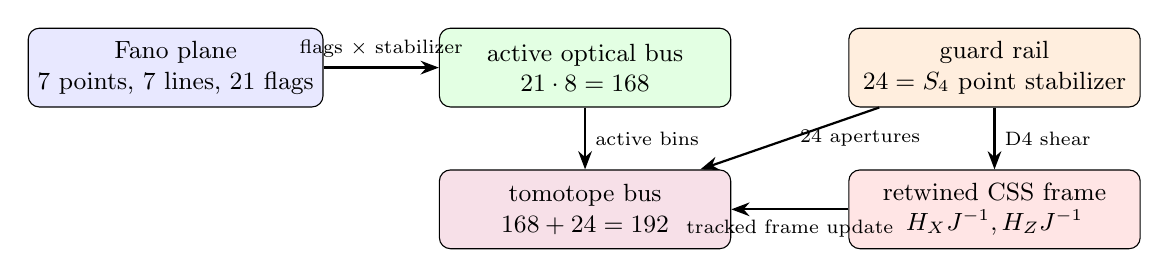
\begin{tikzpicture}[
  every node/.style={font=\small},
  block/.style={draw,rounded corners,align=center,minimum width=37mm,minimum height=10mm},
  arrow/.style={-{Stealth},thick}
]
  \node[block,fill=blue!9] (fano) at (0,0) {Fano plane\\ $7$ points, $7$ lines, $21$ flags};
  \node[block,fill=green!11] (active) at (5.2,0) {active optical bus\\ $21\cdot8=168$};
  \node[block,fill=orange!13] (guard) at (10.4,0) {guard rail\\ $24=S_4$ point stabilizer};
  \node[block,fill=purple!12] (tomo) at (5.2,-1.8) {tomotope bus\\ $168+24=192$};
  \node[block,fill=red!10] (css) at (10.4,-1.8) {retwined CSS frame\\ $H_XJ^{-1},H_ZJ^{-1}$};
  \draw[arrow] (fano) -- node[above,font=\scriptsize]{flags $\times$ stabilizer} (active);
  \draw[arrow] (active) -- node[right,font=\scriptsize]{active bins} (tomo);
  \draw[arrow] (guard) -- node[right,font=\scriptsize]{24 apertures} (tomo);
  \draw[arrow] (guard) -- node[right,font=\scriptsize]{D4 shear} (css);
  \draw[arrow] (css) -- node[below,font=\scriptsize]{tracked frame update} (tomo);
\end{tikzpicture}
\caption{Fano bus closure.  The active 168 detector bins are the Fano flag orbit
with local order-8 stabilizer.  The 24 guard apertures are the tetrahedral point
stabilizer.  The non-Clifford D4 shear is legal only after retwining the CSS
frame.}
\end{figure}

The 211 frontier is also sharpened by this picture.  A packet-symmetric score
above 210 must jump to 212 because the quotient weights are \(10,8,6\).  Thus a
211 witness, if it exists, must split one raw correction slot out of the Fano or
Steinberg packet orbit and must be at S3-gauge radius at least four from the
current incumbent.
%
\begin{center}\small
BT1561--BT1563 record the spiral-qutrit packet: centered OAM basis with mod-three labels, azimuthal/radial/axial factor schema, and falsifier checks for optical mode support and sector correlation.
\end{center}
%
% BT1820 -- Quartet fibre-law paper insert
\subsection{The quartet fibre law}
\label{subsec:quartet-fibre-law}

The residual ternary obstruction in the H27/Schl\"afli transport is not a new global count identity.  It is local.  The $W(E_6)$ stabilizer of the transported eighteen-line image does not fix the observed defect triple uniquely; instead it distinguishes a six-element hinge slice.  Since
\[
  6=\binom{4}{2},
\]
this slice is naturally the edge set of a hidden four-state fibre quartet.

We label the four fibre states by
\[
  \mathbb F_2^2=\{00,01,10,11\}.
\]
Equivalently, this is the local D4/GKP Pauli square
\[
  00\leftrightarrow I,\qquad
  01\leftrightarrow X,\qquad
  10\leftrightarrow Z,\qquad
  11\leftrightarrow XZ.
\]
Under the committed edge-to-hinge chart, the observed support
\[
  (10,22,44)
\]
corresponds to the diagonal quartet edge
\[
  00\longrightarrow 11,
\]
that is, to the simultaneous $XZ$ half-shift in the local fibre square.

The resulting local correction law is:
\[
  \boxed{\text{oriented quartet edge}\;=\;\text{two endpoint losses plus one edge-target gain, in units of }2.}
\]
For the observed edge this gives
\[
  \boxed{T010:-2,\qquad T210:-2,\qquad T222:+2.}
\]
The uncorrected count vector has double-six syndromes
\[
  F_2=(0,0),\qquad F_3=(0,2,1,1,1).
\]
The quartet-edge correction contributes
\[
  F_2=(0,0),\qquad F_3=(0,1,2,2,2),
\]
so the corrected vector satisfies
\[
  \boxed{F_2=(0,0),\qquad F_3=(0,0,0,0,0).}
\]
Thus the binary Hesse delta split is preserved while the ternary double-six obstruction is cancelled.

The search problem is correspondingly reduced:
\[
  816\;\text{triples}
  \longrightarrow 54\;\text{Hesse hinges}
  \longrightarrow 10\;W(E_6)\text{-stabilizer slices}
  \longrightarrow 6\;K_4\text{ edges}
  \longrightarrow 1\;\text{oriented edge}.
\]
This is the operative fibre-law statement: $W(E_6)$ selects the hidden quartet edge-slice, while the remaining orientation is the local $12=3\times4$ fibre datum.
%
% Passes 2825--2828: finite-delay support observer.
\subsection{Finite-delay support observability}
\label{sec:bt2825-bt2828-support-observer}

The PG$(3,2)$ support shell is not an instantaneous execution quotient of the
$81$-state ternary frame, but it is an exact finite-delay observer.  Refinement by all
support observations reachable with words of bounded length gives
\[
 \boxed{16\longrightarrow40\longrightarrow78\longrightarrow81},
\]
with unresolved state-pair counts
\[
 \boxed{272,\;53,\;3,\;0}.
\]
Thus the adaptive/all-word observability index is three.  The three pairs surviving
through depth two are
\[
 (0,0,1,z_f)\sim(0,0,2,z_f),\qquad z_f\in\mathbb F_3,
\]
and all are split by length-three diagnostic words.

A fixed preset experiment requires six operations.  The best numbers of distinct support
trajectories for word lengths one through six are
\[
 \boxed{25,\;40,\;45,\;68,\;77,\;81}.
\]
Exactly eight length-six words are injective.  One canonical word is
\[
 \boxed{
 \mathrm{CX}_{p\to f},\;F_p,\;Z_p,\;F_p,\;Z_p,\;\mathrm{CX}_{p\to f}
 }.
\]

Its seven four-bit support snapshots contain $28$ raw bits.  Exhaustive tap selection
shows that seven taps never suffice, while exactly $48$ eight-tap selectors distinguish
all $81$ states.  A canonical selector uses flattened columns
\[
 \boxed{(0,1,2,5,13,21,25,26)}.
\]
No minimal selector samples the $z_f$ support bit.  Consequently the machine may retain
full ternary phase internally while exposing only binary support telemetry: a six-cycle
diagnostic sequencer, eight one-bit samples, and an $81$-entry ROM recover the exact frame.
The result is noiseless observability; no robustness against loss, detector error, or gate
imperfection is asserted.
%
% Collision-safe wrapper for the two independently frozen Passes 3989--3996 theorem layers.
\section{Passes 3989--3996: physical incidence photon processor}
\label{sec:pass3989-3996}

The W33 point graph admits an exact sparse physical lift.  Let $N$ be the $40\times40$ point--line incidence matrix of $W(3,3)$.  Exact enumeration gives
\[
NN^T=4I+A_{W33}.
\]
Hence a dense twelve-neighbour point Hamiltonian may be generated from an eighty-mode bipartite point--line device with 160 couplings, degree four, and girth eight.  Its spectrum is
\[
-4^1,-\sqrt6^{24},0^{30},\sqrt6^{24},4^1.
\]
With point--line coupling $g$ and bus detuning $\Delta$,
\[
H_{\rm eff}=-\frac{g^2}{\Delta}(A+4I)+O(g^4/\Delta^3),
\]
and $t=\pi\Delta/(2g^2)$ approaches the exact W33 half-period reflection on the point sector.  This is an analytic architecture, not a fabricated device.

Let $B=J-I-A$ and $D=A-B$.  Then $A+B=J-I$ is geometry-blind on the nonuniform sector, while
\[
\operatorname{Spec}(D)=-15^1,5^{24},-7^{15}.
\]
The spectral projectors are
\[
E_{-15}=\frac{(D-5I)(D+7I)}{160}=\frac J{40},
\quad
E_5=\frac{(D+15I)(D+7I)}{240},
\quad
E_{-7}=-\frac{(D+15I)(D-5I)}{96}.
\]
Consequently $\langle D\rangle$ and $\langle D^2\rangle$ determine all three sector populations.  If identical commuting error $C$ enters both arms, then
\[
e^{-it(A+C)}e^{+it(B+C)}=e^{-it(A-B)},
\]
so the dual-geometry echo cancels it exactly.

The maximum-code census is also complete.  The 945-vertex fixed-parent compatibility graph contains exactly 945 maximum $57$-cliques, split into three parent-group orbits
\[
\boxed{945=540+270+135}
\]
with stabilizer orders
\[
\boxed{96,192,384}.
\]
Thus maximum-code uniqueness is false in the fixed-parent problem.  This corrects the earlier division by an order-192 full coordinate stabilizer without first checking parent preservation.

The seven primitive central blocks of the literal $48$-orbital algebra have simple degrees
\[
1,1,2,2,2,3,5.
\]
Their complete central coarse-graining lattice contains
\[
B_7=877
\]
partitions.  Quotienting equal-degree relabelings by $S_2\times S_3$ leaves exactly
\[
\boxed{198}
\]
inequivalent central types.  These are exact central subalgebras, not automatically combinatorial fusions of the 48 orbital relations.

Three further photon constructions follow from the incidence lift.  First, $\operatorname{rank}N=25$, so the bipartite processor contains thirty exact dark modes.  Second, for $L=12I-A$,
\[
V=e^{-i\pi L/4}=I-(1+i)E_{10},
\qquad V^2=U,
\qquad V^4=I,
\]
which gives an exact four-phase internal graph clock.  Third, for a genuine $m$-fold tensor carrier,
\[
\operatorname{rank}(N^{\otimes m})=25^m,
\qquad
\dim\ker(N^{\otimes m})=40^m-25^m,
\]
so the one-side dark fraction is
\[
\boxed{1-(5/8)^m}.
\]
Only $m+1$ nonzero singular shells occur, with multiplicity $\binom mr24^r$ and squared singular value $16^{m-r}6^r$.

The Monster acquisition gate now composes $U_4(2)\to H\to\mathbb M$ class fusions through maximal-subgroup tables and searches only compatible published explicit \texttt{mmgroup} overgroups.  The promoted status remains
\[
\boxed{\texttt{PENDING\_EXPLICIT\_MONSTER\_U42\_WORDS}}
\]
until four portable words pass the exact pair, triple, order-$25{,}920$, object-action, and class-fusion firewalls.  No variable vacuum $c$, literal hidden photon nodes, fabricated hardware, laboratory result, or unobserved remote build is claimed.
%
\section{Sparse W33 photonics and causal-memory closure}
\label{sec:bt3989-3996}

\paragraph{Two sparse coupler realizations.}
Let $A$ be the adjacency matrix of $W(3,3)$.  A forty-mode equal-edge
coupled-mode array obeying
\[
 i\frac{d\psi}{dz}=\kappa A\psi
\]
implements, at $\kappa z=\pi/2$,
\[
 \boxed{e^{-i\pi A/2}=-\frac{I+A}{3}+\frac{2J}{15}.}
\]
This is an exact symmetric involution with row amplitudes $-1/5$ on a
point and its twelve neighbours and $2/15$ on its twenty-seven
nonneighbours.  Uniform fractional interaction error $\epsilon$ has no
linear average-fidelity term:
\[
 F_{\rm pro}=1-3\pi^2\epsilon^2+O(\epsilon^3),\qquad
 F_{\rm avg}=1-\frac{120}{41}\pi^2\epsilon^2+O(\epsilon^3).
\]

A complementary degree-four lift uses the $40\times40$ point--line
incidence matrix $N$,
\[
 NN^{\mathsf T}=4I+A.
\]
Its eighty-mode bipartite graph has 160 edges, girth eight, and spectrum
\[
 -4^1,\;(-\sqrt6)^{24},\;0^{30},\;(\sqrt6)^{24},\;4^1.
\]
For detuned line-bus modes the leading effective Hamiltonian is
\[
 H_{\rm eff}=-\frac{g^2}{\Delta}(A+4I)+O(g^4/\Delta^3).
\]
These are exact matrix and spectral statements, not fabricated-device
claims.

\paragraph{Dual-geometry echo.}
For the complement $B=J-I-A$,
\[
 A+B=J-I,
\]
while $D=A-B$ has spectrum
\[
 -15^1,\quad5^{24},\quad(-7)^{15}.
\]
If the same commuting perturbation $C$ enters both arms, then
\[
 e^{-it(A+C)}e^{+it(B+C)}=e^{-it(A-B)}.
\]
Thus the common arm is geometry-blind on the nonuniform sector and the
difference arm isolates W33-specific contrast.

\paragraph{Complete maximum-code orbit census.}
For the fixed character code $C=[36,6,16]$, the 945 admissible
weight-four words form a degree-624 compatibility graph with maximum
clique size 57.  There are exactly 945 maximum cliques.  Under
$O_6^-(2)\cong U_4(2){:}2$ they split as
\[
 \boxed{540+270+135}
\]
with stabilizers
\[
 \boxed{96,\;192,\;384}.
\]
Every maximum code is $[36,17,4]$, has the same weight enumerator, and
has intersection-two graph
\[
 \operatorname{SRG}(45,16,8,4)\sqcup
 2\operatorname{SRG}(6,4,2,4)
 \cong T(10)\sqcup2T(4).
\]
Uniqueness is false, but the fixed-parent maximum-code problem is
completely classified.

\paragraph{Central fusion lattice.}
The rank-48 algebra has simple degrees
\[
 1,1,2,2,2,3,5.
\]
All 877 partitions of its seven primitive central sectors were
enumerated.  After quotienting by the order-twelve equal-degree
relabeling group, exactly
\[
 \boxed{198}
\]
inequivalent central fusion subalgebras remain.  This does not assert
that every central partition lifts to a fusion of the forty-eight
orbital relations.

\paragraph{Wigner--Smith time as operational memory.}
For a frequency-dependent W33 scattering unitary
\[
 S(\omega)=e^{i\theta(\omega)L_{W33}},
\]
the Wigner--Smith operator is exactly
\[
 \boxed{Q(\omega)=-iS^\dagger\frac{dS}{d\omega}
 =\theta'(\omega)L_{W33}.}
\]
Hence the proper-delay sectors are
\[
 0^1,\qquad(10\theta')^{24},\qquad(16\theta')^{15},
\]
with mean $12\theta'$, variance $12(\theta')^2$, and total trace
$480\theta'$.  This gives a measurable meaning to internal history:
dwell-time and stored-energy sensitivity, not a changed vacuum causal
speed.

For $m$ independent W33 factors, the exact delay-shell polynomial is
\[
 \boxed{(1+24z^{10}+15z^{16})^m.}
\]
The address space has $40^m$ modes, while
\[
 \langle\tau\rangle=12m\theta',\qquad
 \operatorname{Var}(\tau)=12m(\theta')^2.
\]
Therefore
\[
 \boxed{
 \frac{\log_2(40^m)}{\langle\tau\rangle}
 =\frac{\log_2 40}{12\theta'}
 }
\]
is independent of self-similar depth, and the relative delay width is
$1/\sqrt{12m}$.

\paragraph{Dark memory and causal refinement.}
The incidence lift has a thirty-dimensional exact dark sector.  Under
tensor powers,
\[
 \operatorname{rank}(N^{\otimes m})=25^m,
 \qquad
 \dim\ker(N^{\otimes m})=40^m-25^m,
\]
so the dark fraction is $1-(5/8)^m$.  The exact quarter-step
\[
 V=e^{-i\pi L/4}=I-(1+i)E_{10}
\]
has order four and supplies an internal Floquet clock.

A local-interaction causal cone has schematic physical velocity
\[
 v_{\rm int}\lesssim aC_{LR}(\Delta)J/\hbar.
\]
Self-similar refinement preserves the cone only when $aJ$ remains
fixed.  More serial nodes without stronger coupling slow the internal
cone; node density alone neither determines nor raises vacuum $c$.

\paragraph{Monster and evidence boundary.}
The acquisition search now composes class fusions through explicit
Monster maximal overgroups and performs bounded four-generator
\texttt{mmgroup} searches.  No portable $U_4(2)$ words have passed the
full closure, object-action, and character-fusion gates, so no Monster
embedding is promoted.  Fabrication, measured Wigner--Smith delays,
variable vacuum $c$, literal hidden photon nodes, remote CI/PDF success,
and laboratory performance likewise remain unclaimed.
%
%
% BT613 -- Folded Hashimoto / Hodge Flow Insert
% Manuscript-ready insert tying BT605--BT612 to the Master Evolution Axiom.

\subsection{Folded Hashimoto propagation and the protected Hodge endpoint}\label{subsec:folded-hashimoto-hodge-flow}

The directed nonbacktracking carrier of the W33 collinearity graph has a canonical fold onto the W33 point-line Levi flag carrier.  If
\[
B\in\{0,1\}^{480\times480}
\]
is the directed Hashimoto operator on directed W33 edges, define
\[
T:\mathbb R^{480}\longrightarrow \mathbb R^{160}
\]
by
\[
\boxed{
T(p\to q)=(p,\ell(p,q)),
}
\]
where \(\ell(p,q)\) is the unique W33 generalized-quadrangle line through the adjacent points \(p,q\).  Every directed edge has exactly one image, while every Levi flag has exactly three directed-edge preimages.  Hence
\[
\boxed{
TT^T=3I_{160}.
}
\]
Since W33 has valency \(k=12\), the Hashimoto outdegree is
\[
\boxed{
k-1=11.
}
\]
Therefore the folded powers
\[
\boxed{
F_n=TB^nT^T
}
\]
have row sum
\[
\boxed{
3\cdot 11^n.
}
\]
Thus the Ihara scale survives the directed-edge to Levi-flag fold.

Let \(A_0,A_1,A_2,A_3,A_4\) be the distance relations of the Levi flag association scheme.  The cubic folded operator has radial Bose--Mesner projection
\[
\boxed{
\mathcal R(F_3)
=
12A_0+11A_1+\frac{33}{2}A_2+25A_3+28A_4.
}
\]
The lower shells are not fully radial before projection.  Their orientation residuals split as follows:
\[
A_1:\quad 4\;\text{on same-line pairs},\qquad 18\;\text{on same-point pairs},
\]
\[
A_2:\quad 27\;\text{on forward cross-incidences},\qquad 6\;\text{on backward cross-incidences},
\]
\[
A_3:\quad 24\;\text{when the source points are collinear},\qquad 26\;\text{when they are noncollinear}.
\]
But the terminal protected shell has no orientation residual:
\[
\boxed{
F_3\circ A_4=28A_4.
}
\]
Here
\[
\boxed{
28=v-k=40-12=\mu.
}
\]
The distance-four shell has
\[
\boxed{
12960=160\cdot81=1620\cdot8
}
\]
ordered flag pairs, so the cubic folded endpoint has total mass
\[
\boxed{
12960\cdot 28.
}
\]

This gives the finite geometric mechanism behind the evolution axiom.  Raw propagation is the folded Hashimoto process \(F_n=TB^nT^T\).  Physical propagation is obtained by passing this raw nonbacktracking transport through the Hodge/Bose--Mesner projector onto the protected Levi cycle sector
\[
\boxed{
E_4=\frac1{160}CC^T
=I-D^T(DD^T)^+D.
}
\]
Therefore the slogan
\[
\boxed{
\textbf{physical evolution = Hodge projection of Ihara/nonbacktracking propagation}
}
\]
now has a concrete finite operator model:
\[
\boxed{
B\quad\xrightarrow{\;T(-)T^T\;}\quad F_n\quad\xrightarrow{\;\text{Bose--Mesner/Hodge projection}\;}\quad E_4.
}
\]
The important boundary is that the fold is not an unrepaired adjacency intertwiner on all shells.  It is an exact nonbacktracking transfer whose protected endpoint shell is already radial, while lower-shell orientation data must be projected before it becomes physical Hodge data.
%
\subsection{The \texorpdfstring{$E_2$}{E2} duad--phase carrier and the complexified \texorpdfstring{$G_2$}{G2} boundary}
\label{subsec:bt633-e2-duad-phase-carrier}

The full folded-cubic Bose--Mesner action shows that the primitive \(E_2\) sector is internally split:
\[
E_2F_3E_2:\qquad 77^{15}\oplus(-3)^{15}.
\]
Equivalently, the \(E_2\)-block satisfies the quadratic relation
\[
\boxed{x^2-74x-231=0.}
\]
Thus the spectral projectors inside \(E_2\) are
\[
\boxed{P_{77}=\frac{E_2F_3E_2+3E_2}{80},}
\qquad
\boxed{P_{-3}=\frac{77E_2-E_2F_3E_2}{80}.}
\]
Both have rank \(15\).

A natural explicit carrier for this split is the \(K_6\)-duad carrier tensored with a two-sheet phase sign:
\[
\boxed{
\mathbb Q^{15}_{K_6\text{ duads}}\otimes \mathbb Q^2_{\pm}.
}
\]
On this carrier the model operator is
\[
\boxed{B_{E_2}=37I+40\sigma_z.}
\]
Hence
\[
37+40=77,
\qquad
37-40=-3.
\]
This realizes the exact \(15+15\) splitting as a phase-sheet splitting over the \(15\)-duad basis.

This statement should be read with the same boundary as the \(W(G_2)\)-packet obstruction.  The \(K_6\)-duad carrier gives a clean \(15\)-label model for the two rank-\(15\) halves, but it does not by itself prove that the numeric \(E_2\)-eigenbasis has already been canonically identified with the \(K_6\)-duad basis.  That requires an additional intertwiner construction.

Likewise, the \(E_1+E_3\) sector admits an external \(W(G_2)\cong D_6\) organization,
\[
E_1+E_3\leadsto4(G_2^{\rm short})\oplus4(G_2^{\rm long}),
\]
but the folded-cubic cross-channel itself squares to \(-I\) after normalization, not \(+I\).  Therefore it is a quadratic or complex conjugate transport channel.  A real \(W(G_2)\)-reflection obeys \(s^2=+I\), while the folded-cubic channel obeys
\[
\boxed{J^2=-I.}
\]
After adjoining a scalar phase, however,
\[
\boxed{(iJ)^2=+I,}
\]
so a complexified or projective packet model can absorb the sign.  The resulting picture is:
\[
\boxed{
E_2=15_+\oplus15_-,
\qquad
E_1+E_3=24\oplus24,
\qquad
E_4=81\text{ protected Hodge sector}.
}
\]
Thus \(E_2\) carries a duad--phase split, \(E_1+E_3\) carries a complexified \(G_2\)-boundary packet, and \(E_4\) remains isolated as the physical Hodge sector.
%
\subsection{Sentinel admission, two-adic chiral lift, native runtime, and eight-bin photonic compilation}
\label{sec:levi-next5-v2}

The odd-$q$ rank theorem is now represented by an exact symbolic dependency
certificate. The nontrivial additive-character block is
$Y\mapsto Y+Y^T$ on $\operatorname{Mat}_q$, the transformed incidence image is
$\operatorname{Sym}_q$, and the line Gram form retains only diagonal
coordinates in characteristic two. Together with the affine-plane fixed block,
this proves
\[
 \operatorname{rank}_2M_q=\frac{q(q+1)^2+2}{2},\quad
 \operatorname{rank}_2A_P=\frac{q(q^2+1)}2+1,\quad
 \operatorname{rank}_2A_L=q^2+1,
\]
and hence
\[
 D_q\sim J_4^2\oplus J_3^{(q^3+2q^2+q-4)/2}
 \oplus J_1^{q(q-1)^2/2}
\]
with no $J_2$ blocks for every odd prime power $q$.

The Pass--159 sentinel code is now used directly by packet admission. For an
authenticated envelope, the context-readout syndrome is applied to the payload
displacement from the provenance-derived expected packet. Since the code is
$[40,15,8]_2$, every nonzero displacement of support below eight is detected.
A minimum dark-code displacement is still rejected by transition provenance,
and a raw point/line retag is rejected as type confusion.

The chiral two-primary discriminant form admits the exact refinement
\[
 A_2(L_{-4})\cong(\mathbb Z/2)^{14}\oplus\mathbb Z/8.
\]
If $h$ generates the depth-three factor, then
\[
 q(h)=\frac{11}{8}\pmod{2\mathbb Z}.
\]
The natural map $L_{-4}/2L_{-4}\to A_2(L_{-4})[2]$ sends the unique fixed line
to $\langle4h\rangle$, while
\[
 h^\perp\cong U_{14}^-.
\]
The Brown invariants are $7$ and $4$, summing to the previously computed
2-adic phase $3$ modulo eight.

The native runtime is the regular action of
\[
 \PSp(4,3):2\cong W(E_6)
\]
on $51840$ states. The index-two subgroup has two regular chirality orbits of
size $25920$, and the outer similitude swaps them. A point stabilizer has order
$648$, center $3$, and quotient order $216$; a noncollinear-pair stabilizer has
order $48$. Thus
\[
 51840=2\cdot40\cdot3\cdot216=2\cdot540\cdot48,
\]
with unique coordinates given by chirality, point, central phase, and Clifford
quotient class.

Finally, the integral $8\times80$ Levi-to-$E_8$ intertwiner factors through only
eight time bins,
\[
 0,4,7,13,40,41,44,45,
\]
and the active $8\times8$ matrix is unimodular. An exact 16-mode unitary
dilation has a verified 120-rotation Reck netlist; an equivalent Clements mesh
uses 120 Mach--Zehnder elements. The sparse readout realization uses the
support-optimal $86$ tunable couplers and $31$ $\pi$-phase elements. Under the
stated loss and detector model, optical loss becomes retry/no-click and all
modeled dark-count corruptions are rejected by the sentinel/provenance layer.

\emph{Witnesses:}
\path{analysis/w33_levi_next5_v2.py},
\path{data/PART_2026_07_10_LEVI_NEXT5_V2_results.json}, and
\path{tests/test_w33_levi_next5_v2.py}.
%
\subsection{Discriminant automorphisms, native $E_6$ objects, and the optical admission loop}
\label{sec:levi-next5-v3}

The odd-prime-power rank assembly has been translated into a placeholder-free
Lean~4 module, together with a dependency and polynomial-identity certificate.
It formalizes the block-rank sums, parity of the odd-$q$ multiplicity
numerators, and the Jordan rank ladder. The source is pinned to the current
mathlib toolchain; kernel compilation is not claimed in the present execution
environment because Lean and Lake are unavailable there.

For the integral chiral lattice $L_{-4}$, the complete two-primary
discriminant group is
\[
 A_2(L_{-4})\cong(\mathbb Z/2)^{14}\oplus\mathbb Z/8.
\]
Transporting the integral permutation action through exact Smith coordinates
gives a faithful quadratic action of orders $25920$ and $51840$. If $h$ is
the canonical order-eight generator, then $q(h)=11/8$ and the fixed line is
$\langle4h\rangle$. In the canonical elementary generators $e_i$, the outer
involution acts by
\[
 \tau(h)=5h+e_0+e_1+e_2+e_5+e_8+e_{10}+e_{12}+e_{13}.
\]
Thus the outer action is genuinely mixed, not merely fixed or inverted; its
square is the identity and the $\PSp(4,3)$-orbit of $h$ has size $2880$.

The same native generators induce the six-dimensional minus-type homology
module. Its $27$ singular vectors are explicitly identified with the cubic-
surface lines $E_i,L_{ij},Q_i$. Their graph reconstructs $45$ tritangent
planes and $72$ oriented double-sixes, hence the $72$ roots of $E_6$. The
regular $51840$-state runtime maps equivariantly with fibers
\[
 51840/27=1920,\quad 51840/45=1152,\quad
 51840/72=720,\quad 51840/540=96.
\]
The last fiber splits by chirality into two $48$-element middleware fibers.

The normalized eight-bin integral $E_8$ map is compiled into a $16$-mode
Halmos dilation with $120$ two-mode rotations. Exact reconstruction residuals
are below $7\times10^{-15}$. A tolerance model including fabrication offsets,
phase drift, finite extinction, correlated loss, and $50$~ps detector jitter
selects calibration gain $1.025$ and yields
\[
 \overline F=0.999297,\qquad F_{5\%}=0.998749,
\]
compared with uncalibrated $\overline F=0.989727$.

Finally, balanced optical click streams carry the eight-bit point-homology
syndrome. Maximum-likelihood optical decoding reconstructs a $40$-bit cycle,
after which authentication, the $[40,15,8]_2$ sentinel, immutable provenance,
homology validation, retry control, and the native $W(E_6)$ coordinate map run
in sequence. All $256$ noiseless words pass. In $2500$ noisy frames, $2495$
are admitted and $5$ retried, with no wrong admission. The attack suite rejects
all $448$ weight-$1$ through weight-$7$ errors at the sentinel, all $45$ weight-
$8$ dark words at provenance, one raw retag at type checking, and one invalid
tag at authentication.

\emph{Witnesses:}
\path{formal/W33/OddQRank.lean},
\path{analysis/w33_levi_next5_v3_discriminant.py},
\path{analysis/w33_levi_next5_v3_e6.py},
\path{analysis/w33_levi_next5_v3_tolerance.py},
\path{analysis/w33_levi_next5_v3_emulator.py}, and
\path{data/PART_2026_07_10_LEVI_NEXT5_V3_results.json}.
%
%

\end{document}
